%%%%%%%%%%%%%%%%%%%%%%%%%%%%%%%%%%%%%%%%%%%%%%%%%%%%%%%%%%%%%%%%%%%%%%%%
%     LaTeX source code to approximate a NIST Technical report
%	  Instructions for authors: tinyurl.com/techpubsnist
%	DOI watermark will be added on final PDF
% 	Developed by K. Miller, kmm5@nist.gov
%	Last updated: 26-March-2019
%%%%%%%%%%%%%%%%%%%%%%%%%%%%%%%%%%%%%%%%%%%%%%%%%%%%%%%%%%%%%%%%%%%
\documentclass[12pt]{article}
\usepackage{adjustbox}
\usepackage{amsmath}
\usepackage{amsfonts}   % if you want the fonts
\usepackage{amssymb}    % if you want extra symbols
\usepackage{booktabs}
\usepackage{bm}
\usepackage{chemformula}
\usepackage{float}
%\usepackage{fourier}
\usepackage{footnote}
\usepackage{multirow}
\usepackage[hang,flushmargin,bottom]{footmisc} % footnote format

\usepackage{graphicx}   % need for figures
\usepackage{mathptmx}
\usepackage{multicol}
\usepackage{physics}
\usepackage{rotating}
\usepackage{secdot}
\usepackage{siunitx} % Formats the units and values
\usepackage{tabulary}
\usepackage{textgreek}
\usepackage{textcomp}
\usepackage{tikz}
\usepackage[newparttoc]{titlesec}
\usepackage[flushleft]{threeparttable}
\usepackage[utf8]{inputenc}
\usepackage[T1]{fontenc}
\usepackage{xcolor}
\usepackage{footmisc}
\titleformat{\section}{\normalsize\bfseries}{\thesection.}{1em}{}	% required for heading numbering style
\titleformat*{\subsection}{\normalsize\bfseries}

\usepackage{tocloft}	% change typeset, titles, and format list of appendices/figures/tables
\renewcommand{\cftdot}{}	
\renewcommand{\contentsname}{Table of Contents}
\renewcommand{\cftpartleader}{\cftdotfill{\cftdotsep}} % for parts
\renewcommand{\cftsecleader}{\cftdotfill{\cftdotsep}}
\renewcommand\cftbeforesecskip{\setlength{4pt}{}}
\addtolength{\cftfignumwidth}{1em}
\renewcommand{\cftfigpresnum}{\figurename\ }
\addtolength{\cfttabnumwidth}{1em}
\renewcommand{\cfttabpresnum}{\tablename\ }
\setlength{\cfttabindent}{0in}    %% adjust as you like
\setlength{\cftfigindent}{0in}

\usepackage{enumitem}         % to control spacing between bullets/numbered lists

\usepackage[nocfg]{nomencl} % to create nomenclature
\makenomenclature
\newcommand\Nomenclature[2]{\nomenclature[#2]{#1}{#2}}

\usepackage[numbers,sort&compress]{natbib} % format bibliography
\renewcommand{\bibsection}{}
\setlength{\bibsep}{0.0pt}

\usepackage[hidelinks]{hyperref}
\hypersetup{
	colorlinks = true,
urlcolor ={blue},
citecolor = {.},
linkcolor = {.},
anchorcolor = {.},
filecolor = {.},
menucolor = {.},
runcolor = {.}
pdftitle={},%%put title here to auto-fill properties of the PDF
pdfsubject={},%%put abstract here
pdfauthor={}, %%put author list here
pdfkeywords={} %%put keywords here
}
\urlstyle{same}

\usepackage{epstopdf} % converting EPS figure files to PDF

\usepackage{fancyhdr, lastpage}	% formatting document, calculating number of pages, formatting headers
\setlength{\topmargin}{-0.5in}
\setlength{\headheight}{39pt}
\setlength{\oddsidemargin}{0.25in}
\setlength{\evensidemargin}{0.25in}
\setlength{\textwidth}{6.0in}
\setlength{\textheight}{8.5in}

\usepackage{caption} % required for Figure labels
\captionsetup{font=small,labelfont=bf,figurename=Fig.,labelsep=period,justification=raggedright}

%%%%%%%%%%% !!!!!! REQUIRED - FILL OUT METADATA HERE !!!!!!!! %%%%%%%%%%%%%%
%  	Report Number - fill in Report Number sent to you (see info below)
%   DOI Statement - fill in DOI sent to you
%   Month Year - fill in Month and Year of Publication
%%%%%%%%%%%%%%%%%%%%%%%%%%%%%%%%%%%%%%%%%%%%%%%%%%%%%%%%%%%%%%%%%%%%%%%%%%%%%%%%%%%%%%
\newcommand{\pubnumber}{2082, Second Edition}
\newcommand{\DOI}{https://doi.org/10.6028/NIST.TN.2082}
\newcommand{\monthyear}{March 2021}


\newcommand*\chem[1]{\ensuremath{\mathrm{#1}}}

\newcommand\numberthis{\addtocounter{equation}{1}\tag{\theequation}}

%%%%%%%%%%%%%%%%%%%%%%%%%%%%%%%%%%%%%%%%%%%%%%%%%%%%%%%%%%%%%%%%%%%%
%   	BEGIN DOCUMENT
%%%%%%%%%%%%%%%%%%%%%%%%%%%%%%%%%%%%%%%%%%%%%%%%%%%%%%%%%%%%%%%%%%%%
\begin{document}
	\urlstyle{rm} % Format style of \url
	
%%%%%%%%%%%%%%%%%%%%%%%%%%%%%%%%%%%%%%%%%%%%%%%%%%%%%%%%%%%%%%%%%%%%
%   Cover Page is REQUIRED and must contain the information
%	displayed here, at a minimum. Additional artwork may be included
%	(e.g., official project/conference logo, etc.).
%	Pub Number automated based on metadata
%%%%%%%%%%%%%%%%%%%%%%%%%%%%%%%%%%%%%%%%%%%%%%%%%%%%%%%%%%%%%%%%%%%%
	\begin{titlepage}
		\begin{flushright}
%%%%%%%%%%%%%%%%%%%%%%%%%%%%%%%%%%%%%%%%%%%%%%%%%%%%%%%%%%%%%%%%%%%%
% 	Automated based on metadata - delete if not applicable
%%%%%%%%%%%%%%%%%%%%%%%%%%%%%%%%%%%%%%%%%%%%%%%%%%%%%%%%%%%%%%%%%%%%
\LARGE{\textbf{NIST Technical Note \pubnumber}}\\
\vfill
%%%%%%%%%%%%%%%%%%%%%%%%%%%%%%%%%%%%%%%%%%%%%%%%%%%%%%%%%%%%%%%%%%%%
%	Title
%%%%%%%%%%%%%%%%%%%%%%%%%%%%%%%%%%%%%%%%%%%%%%%%%%%%%%%%%%%%%%%%%%%%
\Huge{\textbf{The Structure of Medium-Scale Pool Fires}}\\
\vfill
%%%%%%%%%%%%%%%%%%%%%%%%%%%%%%%%%%%%%%%%%%%%%%%%%%%%%%%%%%%%%%%%%%%%
%	Authors - add complete list of authors, affiliations will be
%   added on title page
%%%%%%%%%%%%%%%%%%%%%%%%%%%%%%%%%%%%%%%%%%%%%%%%%%%%%%%%%%%%%%%%%%%%
\large Ryan Falkenstein-Smith\\
\large Kunhyuk Sung\\
\large Jian Chen\\
\large Kimberly Harris\\
\large Anthony Hamins\\
\vfill
%%%%%%%%%%%%%%%%%%%%%%%%%%%%%%%%%%%%%%%%%%%%%%%%%%%%%%%%%%%%%%%%%%%%
%	The DOI is automated based on metadata.	
%%%%%%%%%%%%%%%%%%%%%%%%%%%%%%%%%%%%%%%%%%%%%%%%%%%%%%%%%%%%%%%%%%%%
\normalsize This publication is available free of charge from:\\
\DOI\\
\vfill
%%%%%%%%%%%%%%%%%%%%%%%%%%%%%%%%%%%%%%%%%%%%%%%%%%%%%%%%%%%%%%%%%%%%
%	NIST LOGO - keep as-is
%%%%%%%%%%%%%%%%%%%%%%%%%%%%%%%%%%%%%%%%%%%%%%%%%%%%%%%%%%%%%%%%%%%%


\includegraphics[width=0.3\linewidth]{NIST-logo}\\


\end{flushright}
\end{titlepage}
\begin{titlepage}
%%%%%%%%%%%%%%%%%%%%%%%%%%%%%%%%%%%%%%%%%%%%%%%%%%%%%%%%%%%%%%%%%%%%
%	Title Page is REQUIRED
%%%%%%%%%%%%%%%%%%%%%%%%%%%%%%%%%%%%%%%%%%%%%%%%%%%%%%%%%%%%%%%%%%%%
\begin{flushright}
%%%%%%%%%%%%%%%%%%%%%%%%%%%%%%%%%%%%%%%%%%%%%%%%%%%%%%%%%%%%%%%%%%%%
%   Publication Series & Number - automated
%%%%%%%%%%%%%%%%%%%%%%%%%%%%%%%%%%%%%%%%%%%%%%%%%%%%%%%%%%%%%%%%%%%%
\LARGE{\textbf{NIST Technical Note \pubnumber}}\\
\vfill
%%%%%%%%%%%%%%%%%%%%%%%%%%%%%%%%%%%%%%%%%%%%%%%%%%%%%%%%%%%%%%%%%%%%
%	Title
%%%%%%%%%%%%%%%%%%%%%%%%%%%%%%%%%%%%%%%%%%%%%%%%%%%%%%%%%%%%%%%%%%%%
\Huge{\textbf{The Structure of Medium-Scale Pool Fires}}\\
\vfill
%%%%%%%%%%%%%%%%%%%%%%%%%%%%%%%%%%%%%%%%%%%%%%%%%%%%%%%%%%%%%%%%%%%%
%	Author Order and Grouping. Always identify the primary author/creator first (s/he does not have to be a NIST author). For publications with multiple authors, group authors by their organizational affiliation. The organizational groupings and the names within each grouping should generally be ordered by decreasing level of contribution.
%	For non-NIST authors, list their city and state below their organization name.
%	For NIST authors, include the Division and Laboratory names (but do not include their city and state).
%%%%%%%%%%%%%%%%%%%%%%%%%%%%%%%%%%%%%%%%%%%%%%%%%%%%%%%%%%%%%%%%%%%%
\normalsize Ryan Falkenstein-Smith\\
Kunhyuk Sung\\
Jian Chen\\
Anthony Hamins\\
\large
\textit{Fire Research Division}\\
\textit{Engineering Laboratory}\\
\vspace{12pt}
\vfill

\normalsize Kimberly Harris\\
\large
\textit{Chemical Science Division}\\
\textit{Material Measurement Laboratory}\\
\vspace{12pt}
\vfill
%%%%%%%%%%%%%%%%%%%%%%%%%%%%%%%%%%%%%%%%%%%%%%%%%%%%%%%%%%%%%%%%%%%%
%   DOI Statement - automated
%%%%%%%%%%%%%%%%%%%%%%%%%%%%%%%%%%%%%%%%%%%%%%%%%%%%%%%%%%%%%%%%%%%%
\normalsize This publication is available free of charge from:\\
\DOI\\
\vfill
%%%%%%%%%%%%%%%%%%%%%%%%%%%%%%%%%%%%%%%%%%%%%%%%%%%%%%%%%%%%%%%%%%%%
%   Date - Month and Year - automated
%%%%%%%%%%%%%%%%%%%%%%%%%%%%%%%%%%%%%%%%%%%%%%%%%%%%%%%%%%%%%%%%%%%%
\normalsize \monthyear
\vfill
%%%%%%%%%%%%%%%%%%%%%%%%%%%%%%%%%%%%%%%%%%%%%%%%%%%%%%%%%%%%%%%%%%%%
%  Department of Commerce LOGO - leave as-is
%%%%%%%%%%%%%%%%%%%%%%%%%%%%%%%%%%%%%%%%%%%%%%%%%%%%%%%%%%%%%%%%%%%%	


\includegraphics[width=0.18\linewidth]{DoC-logo}\\
\vfill
%%%%%%%%%%%%%%%%%%%%%%%%%%%%%%%%%%%%%%%%%%%%%%%%%%%%%%%%%%%%%%%%%%%%
%  Department of Commerce & NIST Leadership
%	will be updated as changes occur
%%%%%%%%%%%%%%%%%%%%%%%%%%%%%%%%%%%%%%%%%%%%%%%%%%%%%%%%%%%%%%%%%%%%
\footnotesize U.S. Department of Commerce\\
\textit{Wilbur L. Ross, Jr., Secretary}\\
\vspace{10pt}
National Institute of Standards and Technology\\
\textit{Walter Copan, NIST Director and Undersecretary of Commerce for Standards and Technology}
\end{flushright}
\end{titlepage}

\begin{titlepage}
%%%%%%%%%%%%%%%%%%%%%%%%%%%%%%%%%%%%%%%%%%%%%%%%%%%%%%%%%%%%%%%%%%%%
%   Disclaimer/CODEN page - required
%%%%%%%%%%%%%%%%%%%%%%%%%%%%%%%%%%%%%%%%%%%%%%%%%%%%%%%%%%%%%%%%%%%%
\begin{flushright}
\footnotesize  Certain commercial entities, equipment, or materials may be identified in this document in order to describe an experimental procedure or concept adequately. Such identification is not intended to imply recommendation or endorsement by the National Institute of Standards and Technology, nor is it intended to imply that the entities, materials, or equipment are necessarily the best available for the purpose.\\
\vfill
%%%%%%%%%%%%%%%%%%%%%%%%%%%%%%%%%%%%%%%%%%%%%%%%%%%%%%%%%%%%%%%%%%%%
%   This secton automated - do not change
%%%%%%%%%%%%%%%%%%%%%%%%%%%%%%%%%%%%%%%%%%%%%%%%%%%%%%%%%%%%%%%%%%%%
\normalsize \textbf{National Institute of Standards and Technology Technical Note \pubnumber\\
Natl. Inst. Stand. Technol. Tech. Note \pubnumber, \pageref{LastPage} pages (\monthyear)} \\
\textbf{CODEN: NTNOEF}\\
\vspace{12pt}
\textbf{This publication is available free of charge from: \DOI}
\vfill
\end{flushright}
\end{titlepage}
%%%%%%%%%%%%%%%%%%%%%%%%%%%%%%%%%%%%%%%%%%%%%%%%%%%%%%%%%%%%%%%%%%%%
%   Start front matter - page number starts with "i"
%%%%%%%%%%%%%%%%%%%%%%%%%%%%%%%%%%%%%%%%%%%%%%%%%%%%%%%%%%%%%%%%%%%%
\section*{Abstract}
This report documents a series of time-averaged gas species measurements made along the centerline of methanol, ethanol, acetone, methane\textcolor{red}{, and propane} pool fires steadily burning in a quiescent environment. All gas species measurements are obtained using a Gas Chromatograph/ Mass Spectrometer System (GC/MS) for gas samples extracted at various heights above the fire and repeated at least twice at each location. Gas species volume fractions are determined via the GC/MS using predetermined calibration factors. Soot mass fractions are simultaneously measured during the gas sampling process. The gas species volume and soot mass fractions are compared at different heights within the fire and across a variety of different fuels. Other fire parameters are measured as well, including time-averaged temperature measurements and mass burning rates.
\section*{Keywords}
\normalsize Acetone, Ethanol, Gas pool fires, Gas species measurements, Methanol, Methane, Liquid pool fires, Propane\\
\pagebreak
%%%%%%%%%%%%%%%%%%%%%%%%%%%%%%%%%%%%%%%%%%%%%%%%%%%%%%%%%%%%%%%%%%%%
%   Table of Contents is required
% 	List of Tables & Figures required if more than 5 tables/figures
%%%%%%%%%%%%%%%%%%%%%%%%%%%%%%%%%%%%%%%%%%%%%%%%%%%%%%%%%%%%%%%%%%%%

\tableofcontents
	
\pagebreak

\listoftables
\pagebreak
\listoffigures

\clearpage
\mbox{}
\nomenclature[01]{$A$}{Peak area}
\nomenclature[02]{$A_{\rm corr}$}{Corrected peak area}
\nomenclature[03]{$\rm C$}{Total number of carbon atoms}
\nomenclature[04]{$C_{\rm vap}$}{Volume fraction of vapors}
\nomenclature[05]{$c_{p_{air}}$}{Specific heat of ambient air}
\nomenclature[06]{$c_{\rm b}$}{Specific heat of thermocouple bead}
\nomenclature[07]{$D$}{Diameter of Pool Fire}
\nomenclature[08]{$D_{\rm b}$}{Diameter of thermocouple bead}
\nomenclature[09]{$\epsilon$}{Thermocouple emissivity}
\nomenclature[10]{$\eta$}{Reciprocal of the local fuel equivalence ratio}
\nomenclature[11]{$g$}{Acceleration of gravity}
\nomenclature[12]{$\Delta H_{c}$}{Heat of combustion}
\nomenclature[13]{$\rm H$}{Total number of hydrogen atoms}
\nomenclature[14]{$h$}{Convective heat transfer coefficient}
\nomenclature[15]{$k_{\rm g}$}{Thermal conductivity of the gas}
\nomenclature[16]{$k_p(t)$}{Instantaneous probe constant}
\nomenclature[17]{$L_{\rm{f}}$}{Mean flame height}
\nomenclature[18]{$\dot{m}$}{Mass burning rate}
\nomenclature[19]{$m_{\rm s}$}{Mass of soot}
\nomenclature[20]{$m_{\rm t}$}{Total mass of gas injected into GC/MS}
\nomenclature[21]{$m_{\rm tot}$}{Total mass of gas sampled}
\nomenclature[22]{$\mu_{\rm air}$}{Dynamic viscosity of air}
\nomenclature[23]{$n_{i}$}{Amount of moles of species i}
\nomenclature[24]{$n_{inj}$}{Amount of moles injected into GC/MS}
\nomenclature[25]{$n_{\rm tot}$}{Total amount of moles}
\nomenclature[26]{$\rm Nu$}{Nusselt number}
\nomenclature[27]{$P$}{Pressure}
\nomenclature[28]{$\Delta P(t)$}{Instantaneous pressure difference}
\nomenclature[29]{$\Delta P_{c}(t)$}{Instantaneous corrected pressure difference}
\nomenclature[30]{$P_\infty$}{Ambient pressure}
\nomenclature[31]{$P_{\rm vap}$}{Vapor pressure}
\nomenclature[32]{$\phi$}{Local equivalence ratio}
\nomenclature[33]{$\rm Pr$}{Prandtl number}
\nomenclature[34]{$\dot{Q}$}{Heat release rate}
\nomenclature[35]{$R$}{Universal gas constant}
\nomenclature[36]{$\rm Re$}{Reynolds number}
\nomenclature[37]{$\rho_{\rm_{air}}$}{Density of air}
\nomenclature[38]{$\rho_{\rm b}$}{Density of thermocouple bead}
\nomenclature[39]{$\rho_{\rm gas}$}{Density of gas}
\nomenclature[40]{$\rho_{\infty_{air}}$}{Density of ambient air}
\nomenclature[41]{$s_i$}{Standard deviation of component i}
\nomenclature[42]{$\sigma$}{Stefan-Boltzmann constant}
\nomenclature[43]{$T$}{Temperature}
\nomenclature[44]{$T_{\rm b}$}{Measured thermocouple bead temperature}
\nomenclature[45]{$T_{\rm g}$}{Gas temperature}
\nomenclature[46]{$T_\infty$}{Ambient temperature}
\nomenclature[47]{$t$}{time}
\nomenclature[48]{$\tau_p$}{Pressure transducer response time}
\nomenclature[49]{$U_{\rm g}$}{Velocity of gas}
\nomenclature[50]{$u_i$}{Uncertainty of component i}
\nomenclature[51]{$\dot{V}$}{Volumetric flow rate}
\nomenclature[52]{$V_{\rm g}(t)$}{Instantaneous gas velocity}
\nomenclature[53]{$V_{\rm s}$}{Volume of sampled gas injected into GC/MS}
\nomenclature[54]{$W_{\rm F}$}{Molecular weight of fuel molecule}
\nomenclature[55]{$\textrm{W}_{i}$}{Molecular weight of species i}
\nomenclature[56]{$\bar{X}_{i}$}{Mean volume fraction}
\nomenclature[57]{$\rm x$}{Number of carbon atoms in the fuel molecule}
\nomenclature[58]{${\rm x}_i$}{Numbers of carbon atoms in the molecule}
\nomenclature[59]{$\bar{Y}_{\rm F}$}{Mass fraction of fuel molecule}
\nomenclature[60]{$\bar{Y}_{i}$}{Mean mass fraction}
\nomenclature[61]{${\rm y}_i$}{Numbers of hydrogen atoms in the molecule}
\nomenclature[62]{$Y_{\rm s}$}{Mass fraction of soot}
\nomenclature[63]{$Z$}{Mixture fraction}
\nomenclature[64]{$z$}{Vertical spatial coordinate}
\nomenclature[65]{$z^*$}{Normalized vertical spatial coordinate}
\begin{multicols}{2} 
\printnomenclature
\end{multicols}
\clearpage
%%%%%%%%%%%%%%%%%%%%%%%%%%%%%%%%%%%%%%%%%%%%%%%%%%%%%%%%%%%%%%%%%%%%
%   Start body of text - page number starts with "1"
%%%%%%%%%%%%%%%%%%%%%%%%%%%%%%%%%%%%%%%%%%%%%%%%%%%%%%%%%%%%%%%%%%%%
\section*{\textcolor{red}{Prefeace to Second Edition}}
\textcolor{red}{The second edition of this technical note contains additional data not presented in the first edition of this report, including data on the structure of two propane pool fires. Specifically, new data is reported on the centerline profiles of temperature, velocity, and chemical species for pool fires burning 20 kW and 34 kW propane gaseous pool fires established on a 37~cm effective diameter water-cooled sintered-metal burner. A description and uncertainty analysis of the velocity measurements are described. Centerline velocity measurements are also provided for the methanol, ethanol, acetone, and methane pool fires.}

\clearpage

\section{Introduction}
\label{sec:intro}
Computational fluid dynamics (CFD) models are an important component of performance-based design in fire protection engineering. A requirement of their acceptance in the design process is that these models be verified and validated, the latter of which involves comparison with experimental measurements. The primary objective of this report is to provide data for use in fire model validation.

A pool fire is a fundamental focus of study in fire science. The fuel surface is isothermal, flat and horizontal, providing a well-defined boundary condition for modeling. Fuel and product species concentrations and temperatures have a significant influence on the heat feedback to the fuel surface, which directly affects the burning rate. A zone of particular interest is the fuel rich-core between the flame and the pool surface, where gas species can absorb energy that would otherwise have been transferred to the fuel surface. Few studies in the literature have reported local chemical species measurements within the flame envelop.

The purpose of this study is to characterize the spatial distribution of the principal chemical species in moderate-scale pool fires steadily burning in a well-ventilated, quiescent environment. Here, methanol, ethanol, acetone, methane\textcolor{red}{, and propane} are the fuels of interest. Contrary to ethanol, acetone, methane, \textcolor{red}{and propane}, fires established using methanol are unusual as no carbonaceous soot is present or emitted. These particular fuels are selected for research since the measurements complement results from previous studies, including analyses of the mass burning rate, the temperature and velocity fields, radiative emission, flame height, and pulsation frequency~\cite{Fisher1987,Hamins2016}.


\clearpage

\section{Description of Experiments}
\label{sec:Experiments}

Descriptions of previous pool fire experiments are found in Refs.~\cite{Hamins2016,Hamins1994,Hamins1991,Hamins1996,Lock2008}. All experiments are conducted under a canopy hood surrounded by a cubic enclosure, 2.5~m on a side, made of a double layer wire-mesh screen (5 mesh/cm) to reduce the impact of room ventilation. All measurements are made once the mass burning rate reaches a steady-state, achieved approximately 10~min and 2~min after ignition for the liquid and gas fuels, respectively.

\subsection{Liquid Pool Burner Setup}
\label{ssec:Liquid_Pool_Burner_Setup}

The circular, stainless-steel burn pan, made from cold rolled steel, has an outer diameter of 30~cm, a depth of 15~cm, and a wall thickness of 1.6~mm. The lip of the burner is positioned 30~cm above the floor. As shown in Fig.~\ref{fig:Pool Burner}, the burner is placed within an overflow basin, which extends 3~cm beyond the burner wall.  The bottom of the burner is maintained at a constant temperature by flowing water (approximately $20 \; ^\circ \hbox{C} \pm 5 \; ^\circ \hbox{C}$) through the basin. A fuel level indicator is positioned near the center of the burner to maintain a consistent surface level.

\begin{figure}[h!]
	\centering
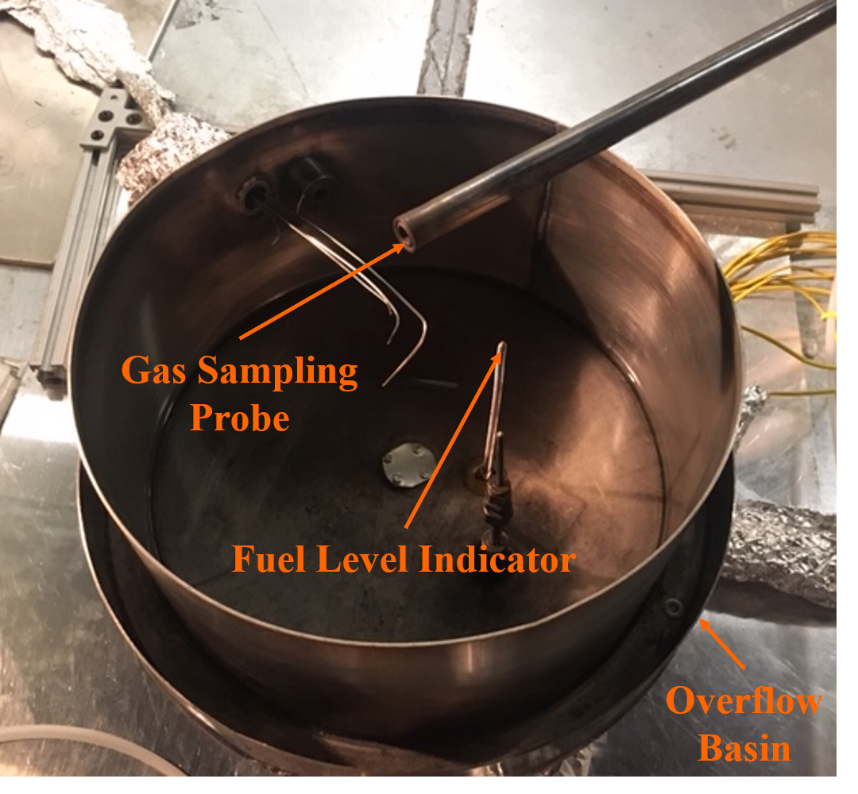
\includegraphics[width=10.0cm,keepaspectratio]{Pool_Burner.png}
	\caption[Photograph of the burner]{The 30~cm burner with fuel level indicator, overflow section, and quenching probe}
	\label{fig:Pool Burner}
\end{figure}

Fuel to the burner is gravity fed from a reservoir positioned on a mass load cell located outside the enclosure and monitored by a data acquisition system (DAQ). As shown in Fig.~\ref{fig:Fuel_Level}, the fuel level is monitored via a fuel flow operator. The operator is able to observe a close up of a slightly discernible dimple (approximately \SI{2}{mm}) made from the fuel level indicator on the fuel surface using a live video feed. The fuel level is controlled by manually adjusting the fuel flow using a needle valve. The fuel surface is maintained \SI{10}{mm} below the burner rim to match previous experimental conditions \cite{Fisher1987,Hamins2016,Kim2019,Weckman1996}.

\begin{figure}[h!]
	\centering
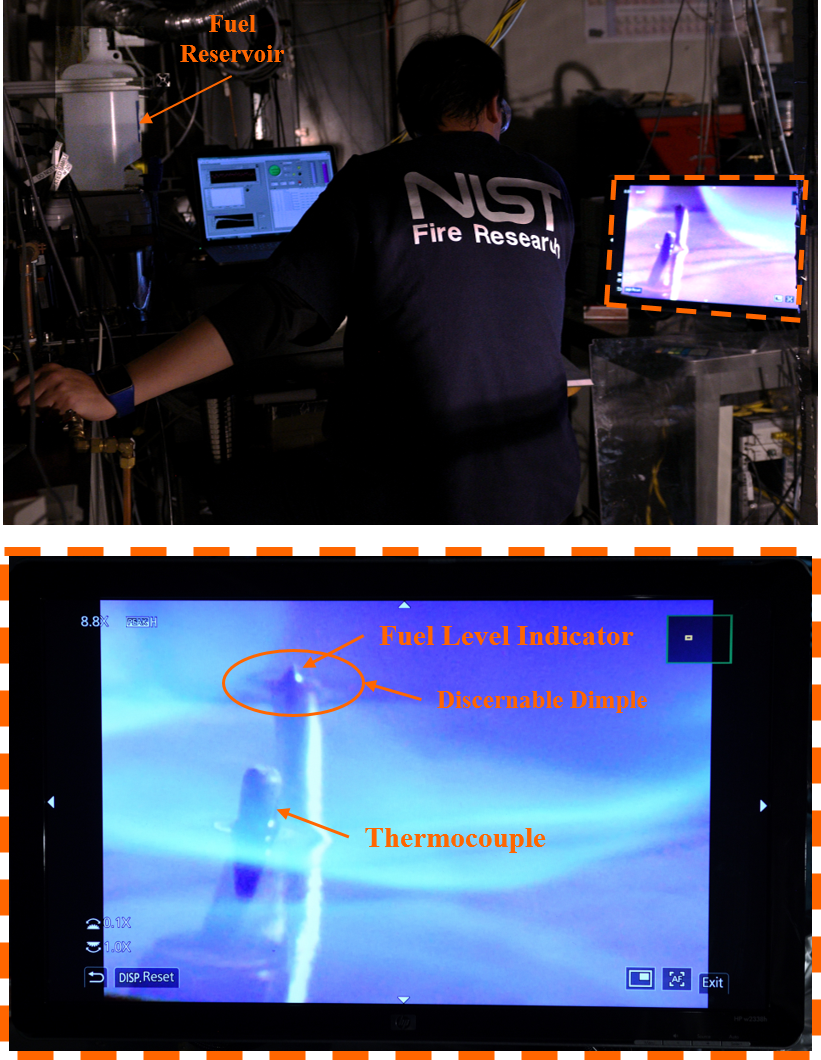
\includegraphics[width=14.0cm,keepaspectratio]{Monitoring_Fuel_Level_A.png}
	\caption[Photographs of the fuel monitoring process]{Photo of fuel flow operator monitoring the fuel level via live video feed (top) and a magnified image of the live video feed used to maintain a consistent fuel level relative to the fuel level indicator (bottom)}
	\label{fig:Fuel_Level}
\end{figure}

\subsection{Gas Pool Burner Setup}
\label{ssec:Gas_Pool_Burner_Setup}
Gas fuels are burned using a \textcolor{red}{burner with an effective diameter of 37~cm}. Fuel to the gas burner is controlled via a \textcolor{red}{Brooks mass flow controller, Model 5863}\footnote{\label{fn:product} Certain commercial products are identified in this report to specify adequately the equipment used. Such identification does not imply a recommendation by the National Institute of Standards and Technology, nor does it imply that this equipment is the best available for the purpose.} located outside of the enclosure. Similar to the liquid pool burner, the gas burner is maintained at a constant temperature by circulating cooled water (approximately $20 \; ^\circ \hbox{C} \pm 5 \; ^\circ \hbox{C}$) through the basin.

\subsection{Measuring Flame Characteristics}
\label{ssec:Flame_Characteristics_Measurements}

The heat release rate, $\dot{Q}$, is the product of the time-averaged mass burning rate, $\dot{m}$, and the heat of combustion, $\Delta H_{c}$:
\begin{equation}\label{eq:Heat_release_rate}
\dot{Q}= \dot{m}~\Delta H_{c}
\end{equation}
The heat of the combustion is provided by Ref.~\cite{Dippr} and reported in Table~\ref{tab:Pool_Fire_Parameters_Table}.

The mean flame height, $L_{\rm{f}}$, is estimated from 3600~frames of high-resolution video of the experiments using MATLAB’s Image Processing Toolbox. Imported color images are decomposed into binary (i.e., black and white) images using a pre-set threshold level. The flame height for a single frame is defined as the distance between the pool surface and flame tip. All measurements are repeated, then averaged to provide the mean flame height. A description of the uncertainty analysis for the mean flame height is described in Appendix~\ref{ssec:Mean_Flame_Height}.

\subsection{Centerline Temperature Measurements}
\label{ssec:Temperature_Measurements}

Time-averaged temperature measurements are made along the vertical centerline of the fire plumes using S-type (Pt 10\% Rh/Pt), bare-wire, fine diameter thermocouples (OMEGA P10S-001) with wire diameters of approximately 13~$\mu$m and 25~$\mu$m for the liquid and gas pool fires, respectively, and bead diameter approximately three times greater. Temperature measurements are sampled at \SI{250}{Hz} for \SI{2}{min}, or approximately 300~pulsing cycles \cite{Wang2019}. The uncertainty of the temperature radiative measurements are discussed in Appendix~\ref{sec:Uncertainty_Temperature_Measurements}. \textcolor{red}{In some cases, temperature measurements are made using thermocouple of different configurations. Thermcouple bead temperature readings of bead diameters for each fuel are presented in Appendix~\ref{sec:Bead_Temp}.}

The measured thermocouple temperatures are corrected for heat losses and thermal inertia using the formula described by Shaddix~\cite{Shaddix1999}:
\begin{equation}\label{eq:Thermocouple_Bead_Correction}
   {T_{\rm g}(t)}= T_{\rm b}(t) + \tau \, \frac{{\rm d}T_{\rm b}}{{\rm d}t} + \frac{\epsilon\sigma}{h}\left(T_{\rm b}(t)^4-T_\infty^4\right)
\end{equation}
where $T_{\rm g}$ is the ``true'' gas temperature, $T_{\rm b}$ is the measured bead temperature, $T_\infty$ is the ambient temperature, $\sigma=5.67 \times 10^{-11} \; {\rm kW}/({\rm m}^2{\rm K}^4)$ is the Stefan-Boltzmann constant, $\epsilon$ is the thermocouple emissivity, and $h$ is the convective heat transfer coefficient. The temperature-dependent emissivity of the platinum is taken from Ref.~\cite{Shaddix1999} and shown below:
\begin{equation}\label{eq:epsilon}
\epsilon=-0.1+\num{3.24e-4} \, T - \num{1.25e-7} \, T^2 \, + \num{2.18e-11} T^3
\end{equation}
$h$ and $\tau$ are defined:
\begin{equation}\label{eq:h_eqn}
h=\frac{{\rm Nu} \, k_{\rm g}}{D_{\rm b}}  \quad ; \quad \tau= \frac{\rho_{\rm b} \, c_{\rm b} \, {D_{\rm b}}^2}{6 \, {\rm Nu} \, k_{\rm g}}
\end{equation}
where $k_{\rm g}$ is the thermal conductivity of the gas, $\rho_{\rm b}$, $c_{\rm b}$, and $D_{\rm b}$ are the density, specific heat, and diameter of the bead, respectively. The thermal conductivity of the gas is determined from datasets provided in Ref.~\cite{Touloukian1970}. The density of the thermocouple bead is assumed constant at 21.45~g/cm~\cite{Platinum2010}. The specific heat of the bead is calculated from the formulae provided in Ref.~\cite{Jaeger1939}. The Nusselt number, Nu, is calculated using the Ranz-Marshall correlation~\cite{Shaddix1999}:
\begin{equation}\label{eq:Nu_number}
{\rm Nu} = 2 + 0.6 \, \textrm{Re}^{1/2} \, \textrm{Pr}^{1/3} \quad ; \quad \textrm{Re} = \frac{ \rho_{\rm air} \, U_{\rm g} \, D_{\rm b} }{\mu_{\rm air}}  \quad ; \quad \textrm{Pr}=0.7
\end{equation}
The temperature-dependent gas properties for Reynolds number, Re, and Prandtl number, Pr, are taken as those of air from Ref.~\cite{Incropera2007}. The gas velocity is assumed to be equal to 2~m/s. The corrected temperature is relatively insensitive to gas velocities between 1~m/s and 3~m/s, consistent with the results of Shaddix~\cite{Shaddix1999}.

The uncertainty of Eq.~(\ref{eq:Thermocouple_Bead_Correction}) is discussed in detail in Ref.~\cite{Sung2019}. This correction formula is included for the convenience of mathematical modeling.

\subsection{Centerline Velocity Measurements}
\label{ssec:Velocity_Measurements}
\textcolor{red}{A bi-directional probe is located above the burner centerline and moved using a computer controlled translation device. A full description of the measurement and data processing methods is given in Ref.~\cite{Sung2021}. The pressure difference between the front and rear side of the probe (16~mm outer diameter and 2.5~cm  long) is measured with multiple pressure transducers with various instrument response times. The instantaneous gas velocity ($V_{\rm{g}}(t)$) can be determined from the instantaneous measured pressure difference between the front and rear sides of the probe and the local gas density:}
\begin{equation}\label{eq:Vel_g}
V_{\rm{g}}(t) = \frac{1}{k_p(t)}\sqrt{\frac{2~\Delta P_{c}(t)}{\rho(t)}}
\end{equation}
\textcolor{red}{where $\Delta P_c(t)$ and $\rho(t)$ are the instantaneous corrected pressure difference and gas density, respectively. The instantaneous gas temperature $ {T_{\rm g}(t)}$ measured near the probe. The parameter $k_p(t)$ is the instantaneous probe constant, whose value depends on several factors, such as Reynolds number, probe shape, and flow approach angle. The temperature-dependent gas properties are taken as those of air.}
\begin{figure}[h!]
	\centering
\includegraphics[width=\textwidth,keepaspectratio]{Vel_probe.png}
	\caption[Photograph of a bi-directional probe]{Photograph of a bi-directional probe with a Type S, 25 µm wire diameter, bare-bead thermocouple positioned a few cm above the water-cooled, sintered-metal, 37 cm diameter, gas burner.}
	\label{fig:Vel_Probe}
\end{figure}
\textcolor{red}{As many as three transducers are used for any single time series pressure measurement. The measurements were repeated at least once and typically twice. A Type S (Pt 10 \% Rh/Pt), 25~µm diameter, bare-wire, thermocouple is positioned 5 mm upstream of the probe as seen in Figure 4. The thermocouple bead is nearly spherical with a bead diameter of approximately 125 µm as determined using optical microscopy. Voltage signals from the pressure transducers and the Type S temperature are obtained using a DAQ (Model: SCXI-1600, National instrument Inc). Data sampling rates are either 250 Hz or 500 Hz, depending on the case. Data is acquired for 2 min at each position along the axial centerline above the burner.}
\textcolor{red}{The instantaneous measured pressure difference is corrected to consider the instrument time response, which is treated in a manner similar to the inertia correction in the thermocouple measurement. The instantaneous corrected pressure difference is defined as:}
\begin{equation}\label{eq:Delta_Pc}
\Delta P_c~(t) = \Delta P(t)+\tau_{p}\frac{d(\Delta P(t))}{dt}
\end{equation}
\textcolor{red}{where the second term on the right side of the equation is the instantaneous time-response correction term. Solving for the correction term, the time derivative of the pressure difference is calculated using a second-order polynomial fit using three consecutive data points in the pressure difference time series. The parameter, $\tau_p$, is the pressure transducer instrument response time. This parameter is experimentally determined for each transducer by applying a step-function pressure change and observing the transient signal response as discussed in Ref.~\cite{Sung2021}}.

\subsection{Measuring the Volume Fraction of Gas Species via GC/MS}
\label{ssec:Gas_Species_Setup}

Figure~\ref{fig:Experimental_Setup} displays the flow diagram for gas and particulate sampling. The GC/MSD is equipped with a 2~mL sample loop maintained at approximately \SI{200}{\degree C}. \textcolor{red}{The characteristic length of the regime of influence was estimated to range between 0.5~cm~$\pm$~0.1~cm to 3.9~cm~$\pm$~0.7~cm. The characteristic length of the regime of influence was calculated using through the approximation provided in Appendix~\ref{sec:Regime_of_Influence}.} The gases are extracted by a vacuum pump located downstream of the GC/MSD. Gas samples are collected using a thermal quenching probe composed of concentric, stainless-steel tubes with outer annular coolant flow and inner extracted sample flow. The outer and inner tube diameters are \SI{16}{mm} and \SI{8}{mm}, respectively. Water at approximately \SI{90}{\degree C} flows through the sampling probe for the duration of the experiment. The remainder of the sampling line leading into the GC/MSD is heated to approximately \SI{140}{\degree C} with electrical heating tape to prevent condensation of water and other condensable species (e.g., methanol, ethanol, benzene, etc.).

\begin{sidewaysfigure}[!]
	\centering
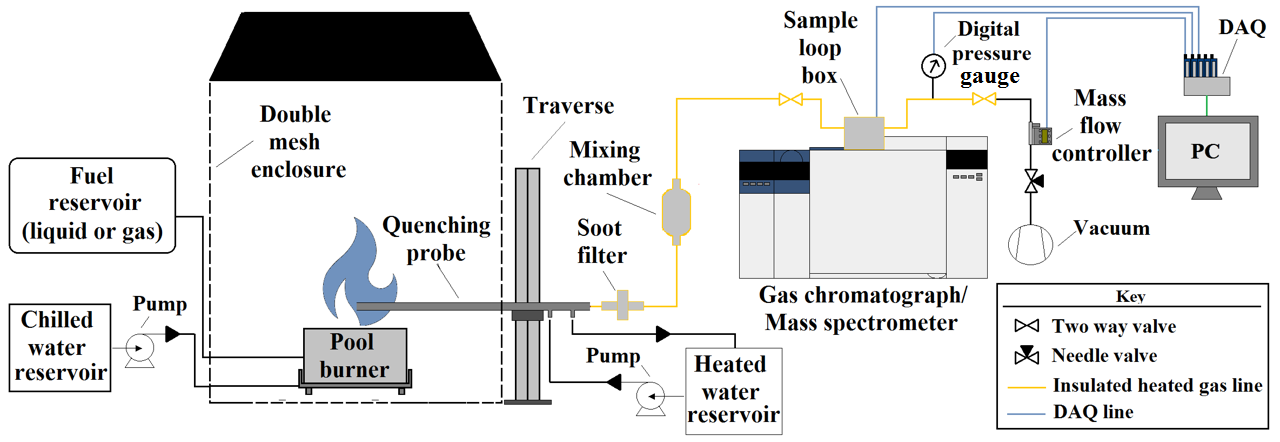
\includegraphics[width=\textwidth,keepaspectratio]{Experimental_Setup.png}
	\caption[A schematic of the gas sampling procedure]{A schematic of the extraction sampling setup used to transport gas samples from the pool fire to the GC/MS.}
	\label{fig:Experimental_Setup}
\end{sidewaysfigure}

\textcolor{red}{Directly behind the sampling probe is a heated soot filter which was used to make a gravimetic soot measurement and eliminate soot from the gas sample injected into the GC. An in-line, heated, 150~ml chamber helps to ensure that the sample is well-mixed and representative of the local sampling volume. Depending on the probe's lateral location within the fire, the sampling period varies from \SI{12}{min} to \SI{25}{min}, ensuring a significant soot measurement is made and that the gases are representative of the sampling location and have completely swept through the sample loop. The sample flow is controlled using a mass flow controller (Alicat Scientific MC-Series) located in upstream of the vacuum pump in the sampling line. All measurements are replicated at least two times to provide an average concentration measurement.}

\textcolor{red}{During the gas sampling procedure, the volumetric flow is approximately 200~mL/min and recorded at \SI{2}{\hertz}. The characteristic length of the regime of influence was estimated to range between 0.5~cm~$\pm$~0.1~cm to 3.9~cm~$\pm$~0.7~cm. The characteristic length of the regime of influence was calculated using through the approximation provided in Appendix~\ref{sec:Regime_of_Influence}. After the gas sampling period, two quarter-turn valves located on opposite ends of the sample loop are closed, at which point pressure measurements, obtained from a digital pressure gauge (OMEGA DPG409-030DWU), and temperature measurements, acquired by a K-type thermocouple located at the GC/MSD sample loop injection port, are collected at \SI{2}{\hertz} for \SI{50}{s} directly followed by sample injection.}

\textcolor{red}{Gas species measurements are made using an Agilent 5977E Series GC/MSD. The GC/MSD quantifies a variety of stable reactant, intermediate, and product species collected from the fire plume using helium as the carrier gas. The GC/MSD utilizes an Agilent J\&W Select Permanent Gases/\ch{CO2} High-Resolution column, which separates permanent gases (i.e., gases that are incapable of liquefaction). As shown in Fig.~\ref{fig:GC_Intern}, the column is a parallel configuration consisting of a 25~m x 0.32~mm PoraBOND Q capillary column coupled with a 50~m x 0.53~mm Molsieve $\SI{5}{\angstrom}$ capillary column. The PoraBOND has high retention for several species, including carbon dioxide, but struggles to separate oxygen, nitrogen, and other species resulting in a single composite peak. The Molsieve $\SI{5}{\angstrom}$ column includes zeolite-based materials with a pore size of $\SI{5}{\angstrom}$, allowing for separation and very high retention of permanent gases. Due to the multi-component setup of the column, some species (e.g., methane or propane) are observed to elute twice from the composite column causing two distinct peaks on the chromatogram.}

\begin{figure}[h!]
	\centering
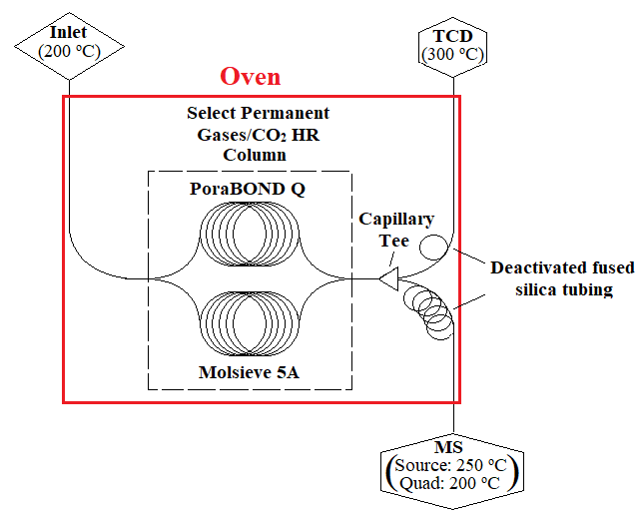
\includegraphics[width=8.45cm,keepaspectratio]{GC_Internal.png}
	\caption[A schematic of the internal plumbing system in the gas chromatograph]{An internal schematic of the GC detailing the column configuration and extension tubing feeding into the detectors.}
	\label{fig:GC_Intern}
\end{figure}

\textcolor{red}{The sample components elute from the column through a capillary tee splitter (Agilent G3184-60065), which divides the flow into two deactivated fused silica tubes (Agilent 160-2615-10) of different lengths leading to the thermal conductivity (TCD) and mass selective detectors. The deactivated fused silica tubing flowing into the TCD and MSD are cut to 1~m and 5~m to maintain carrier gas flows of approximately 3~mL/min $\pm$ 5\% and 1~mL/min $\pm$ 5\%, respectively, such that the TCD and MSD chromatograms are synchronized. Gas species are identified using the total ion chromatogram generated by the MSD and quantified from the TCD's chromatogram.}

For the ethanol, acetone\textcolor{red}{, methane, and propane} pool fires, the sample analysis time is approximately \SI{60}{min}, during which time the GC oven temperature is maintained at \SI{30}{\degree C} for \SI{10}{min}, then ramped at \SI{8}{\degree C/min} for \SI{34}{min} until reaching a temperature of \SI{300}{\degree C} which is maintined for the remainder of the analysis. For methanol pool fires, GC oven has same setpoint temperature hold time and ramp rate, but only ramps to \SI{192}{\degree C} to reduce overall analysis time. During the sample analysis, the TCD is maintained at \SI{300}{\degree C} with a makeup and reference flow of 12~mL/min and 27~mL/min, respectively. Additionally, the MS source and quad temperatures are \SI{250}{\degree C} and \SI{200}{\degree C}, respectively, for the duration of the sample analysis.

A typical TCD chromatogram is shown in Fig.~\ref{fig:Chromatogram}. \textcolor{red}{The elution times for individual gas species are provided in Appendix~\ref{sec:Elution Times}}. The area associated with each peak is proportional to the number of moles of a particular species. Peaks are manually integrated using the Agilent software. Integration bounds of each peak are determined using the MS. In instances where peaks overlap, it is necessary to implement a tangential ``skim'' to improve integration resolution of an overlapping region, as shown in Fig.~\ref{fig:Chromatogram}.

\begin{figure}[h!]
	\centering
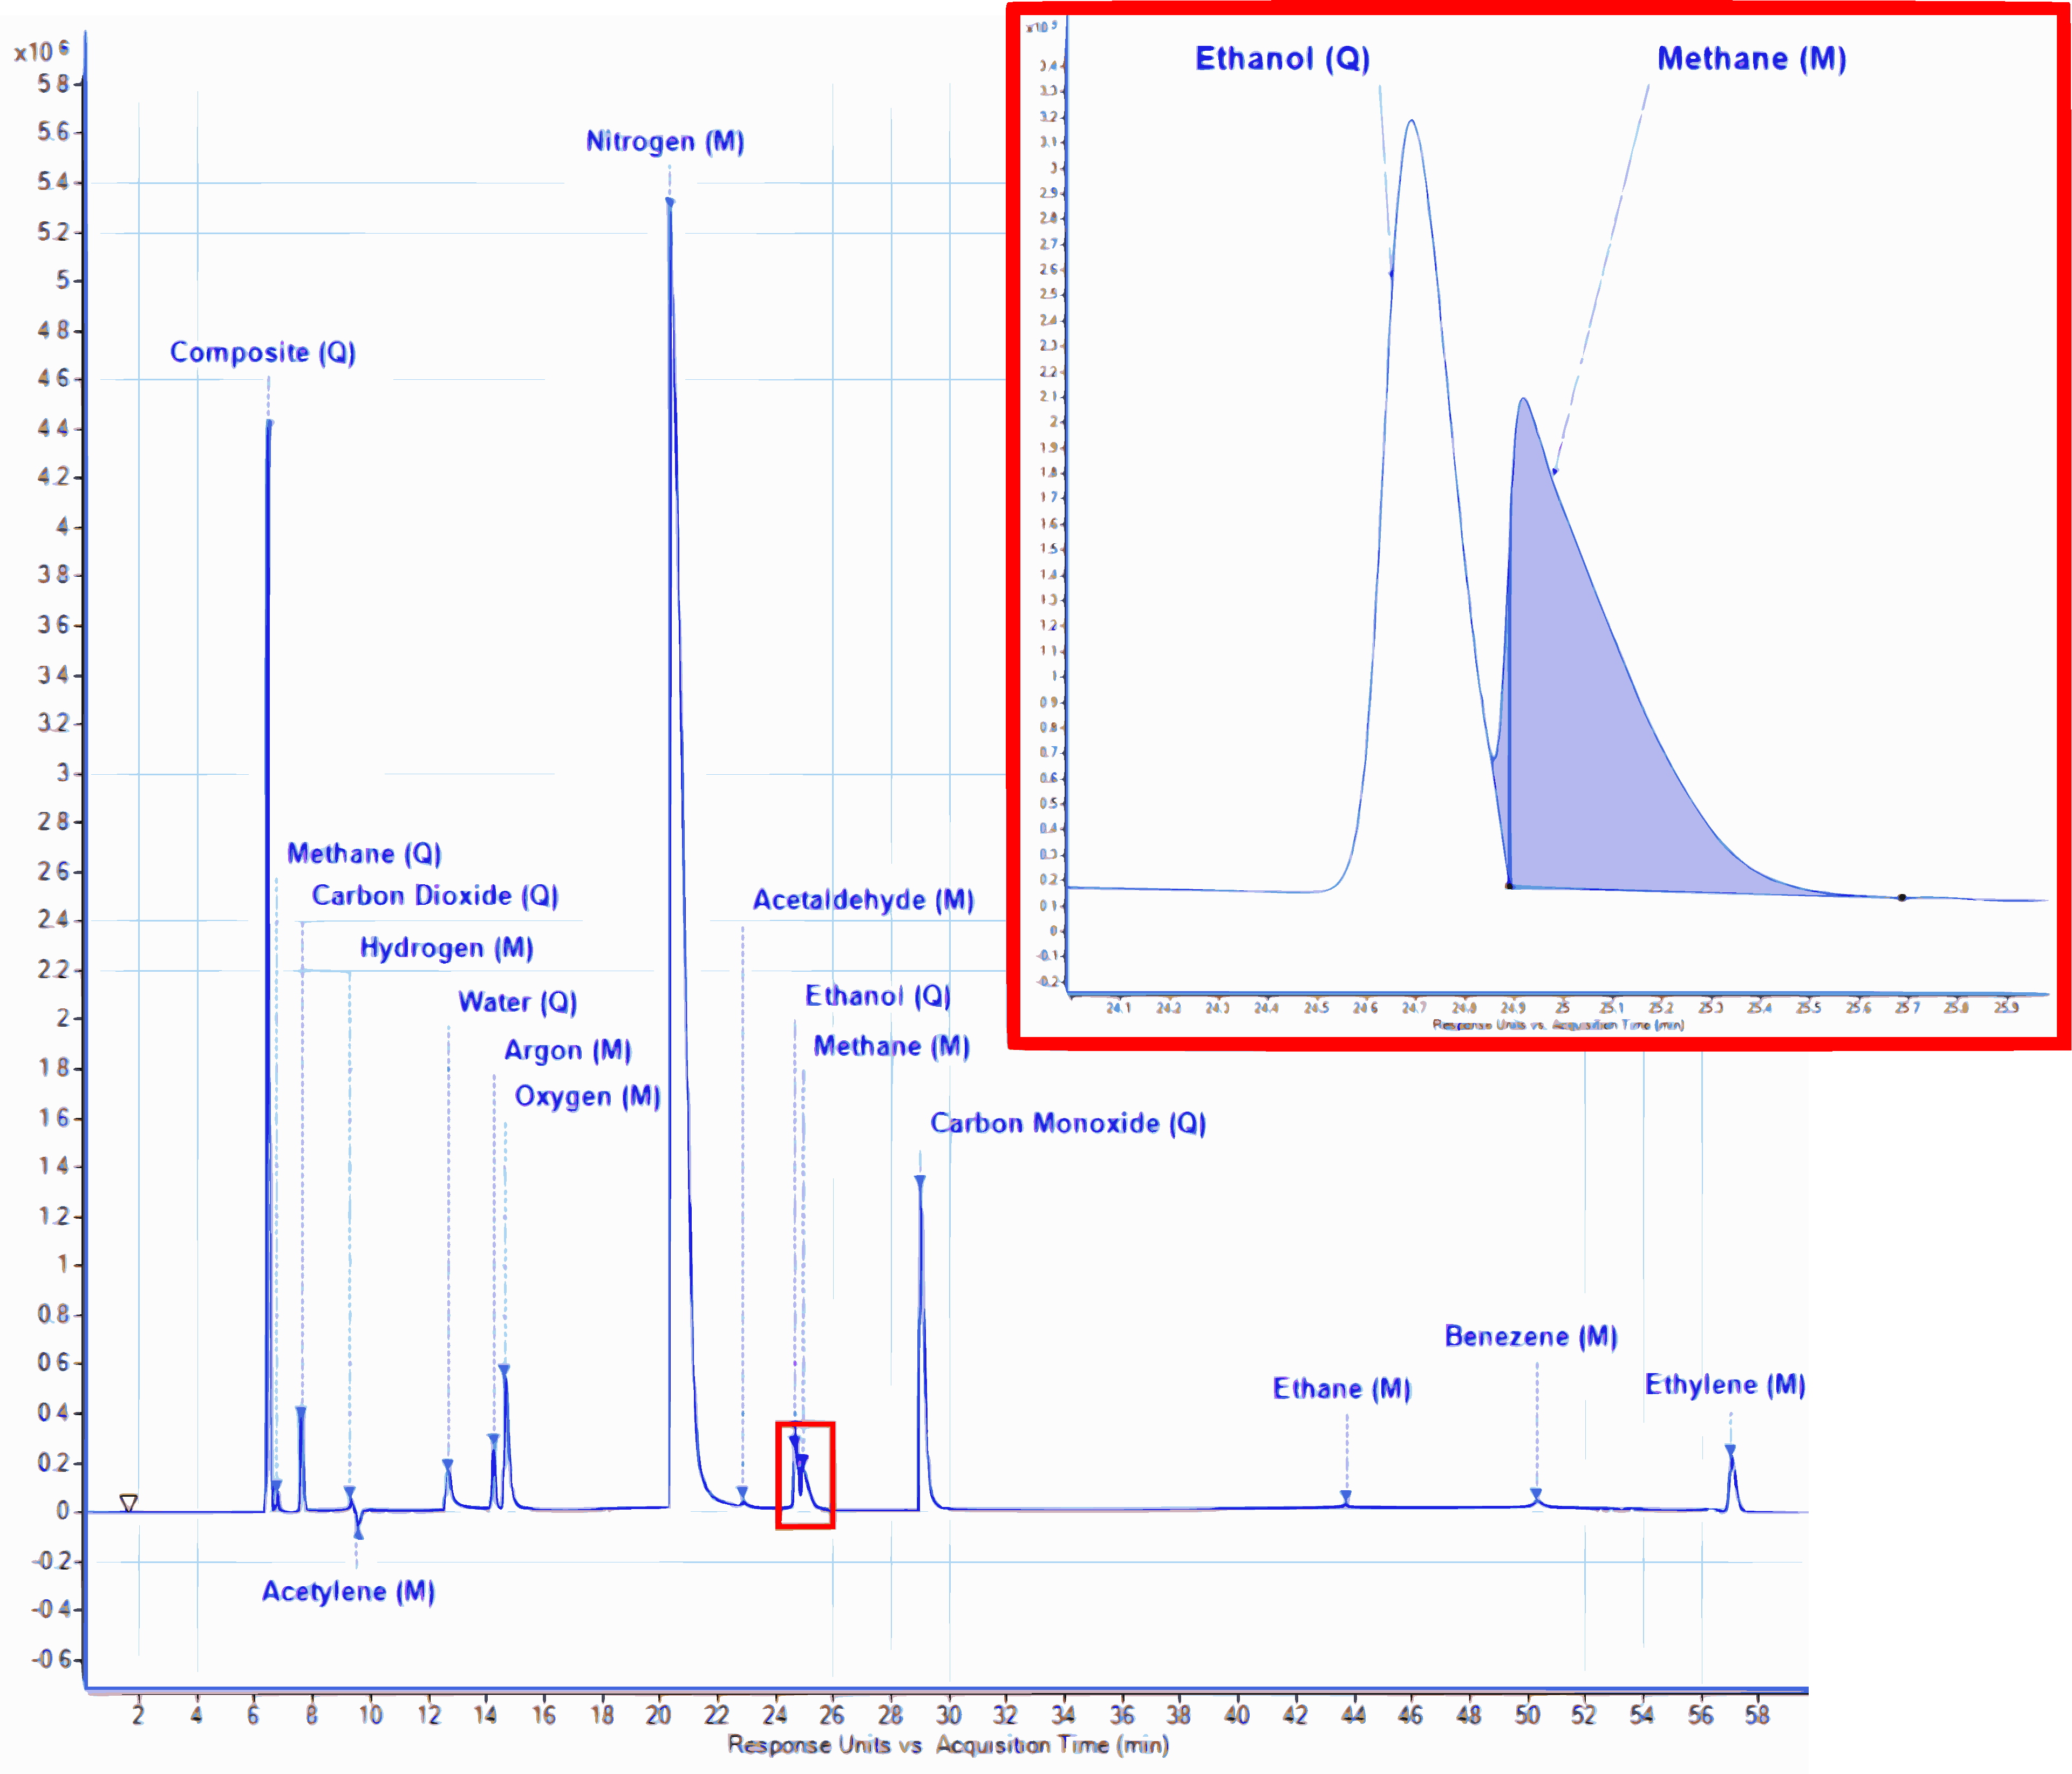
\includegraphics[width=\textwidth,keepaspectratio]{Chromatogram.png}
	\caption[Chromatogram of a pool fire gas sample]{TCD chromatogram of a pool fire gas sample and a magnified image of overlapping peaks with an example of tangential skim integration technique used to determine peak area}
	\label{fig:Chromatogram}
\end{figure}

The area associated with a peak, $A$, is adjusted to account for the variation in the measured pressure, $P$, and temperature, $T$, of the sample:
\begin{equation}\label{eq:Area_corrected}
	A_{\rm corr} = A \, \left(\frac{P \, T_\infty}{P_\infty \, T} \right)
\end{equation}
The corrected area is converted into number of moles using a linear calibration curve determined using gas standards listed in Appendix~\ref{sssec:Table of Gas Standards with Error}. The calibration functions of liquid-vapors (e.g., water, methanol, ethanol, acetone) are obtained from a bubbler apparatus described in Appendix~\ref{sssec:Concentration of Vapors from Bubblers}.

Once the number of moles for all detected species is determined, the volume fraction of each species can be calculated. The mean volume fraction of a given species, $\bar{X}_{i}$, is the ratio of the number of moles of a given gas species, $n_{i}$, and the total number of moles identified by the GC/MS, $n_{\rm tot}$, averaged over the repeated GC/MS gas injections. The total number of moles is determined from the summation of moles for each species quantified from the TCD chromatogram. In the case of water, the relative humidity measured within the room accounted for when calculating its volume fraction.
\begin{equation}\label{eq:volume_fraction}
  	\bar{X}_{i}= \frac{n_{i}}{n_{\rm tot}}
\end{equation}
The mean mass fraction, $\bar{Y}_{i}$, of a given species $i$ is calculated from the measured volume fraction, $\bar{X}_{i}$, using the following expression:
\begin{equation}\label{eq:mass_fraction}
	\bar{Y}_{i}=\frac{\bar{X}_{i} \, {\textrm{W}_{i}}}{\sum{\bar{X}_{i} \, {\textrm{W}_{i}}}}=\frac{\bar{X}_{i} \, {\textrm{W}_{i}}}{W_{\rm{tot}}}
\end{equation}
where ${{\textrm{W}_{i}}}$ is the molecular weight of a given species.

All measurements using the GC/MS are repeated at least twice at each location along the centerline of the pool fire. Gas species concentration measurements made at the same location are averaged. The variance in the volume fraction is a function of position and species. The uncertainty of the species measurements and the calibration procedure is discussed in Appendices~\ref{sec:UncertaintyGasSpecies} and \ref{sec:Uncertainty Analysis of Gas Species Calibrations}, respectively.

\subsection{Determining Soot Mass Fraction}
\label{ssec:Soot_Setup}

Soot mass fraction, $Y_{\rm s}$, is measured using a well established gravimetric technique~\cite{Choi1995}. Soot is filtered out of the gas stream using a stainless steel particulate filter holder (PALL 2220).  Before an experiment, a desiccated \SI{47}{mm} polytetrafluoroethylene (PTFE) filter is weighed and placed into its holder. The filter holder is positioned within the gas sampling line behind the quenching probe and heated with tape to approximately \SI{140}{\degree C} to prevent condensation of water and liquid fuels on the filter. After sampling, the filter is removed and dried in a desiccator. After drying for 48~h, the filter’s final weight is measured. Approximately \SI{1}{mg} of soot is collected during the sampling period, which varies from 12~min to 25~min depending on the sampling location. The mass of the PTFE filter and cleaning patches are measured three times before and after each test\footnote{After some experiments, soot deposits are observed on the inner walls of the quenching probe. As shown in Fig.~\ref{fig:Soot_Probe_Setup}, dedicated gun cleaning patches (Hoppe's 9 1203S) are used to clean the inside of the quenching probe with no cleaning solvent. At least two patches are used to collect soot on the inside of the probe. A petri dish is placed below one end of the probe to catch dislodged soot and patches. Soot collection on the inside of the probe concludes once an applied patch is observed to have no soot. Patches are weighed before and 48~h after cleaning the inside of the probe.}.

\begin{figure}[ht!]
	\centering
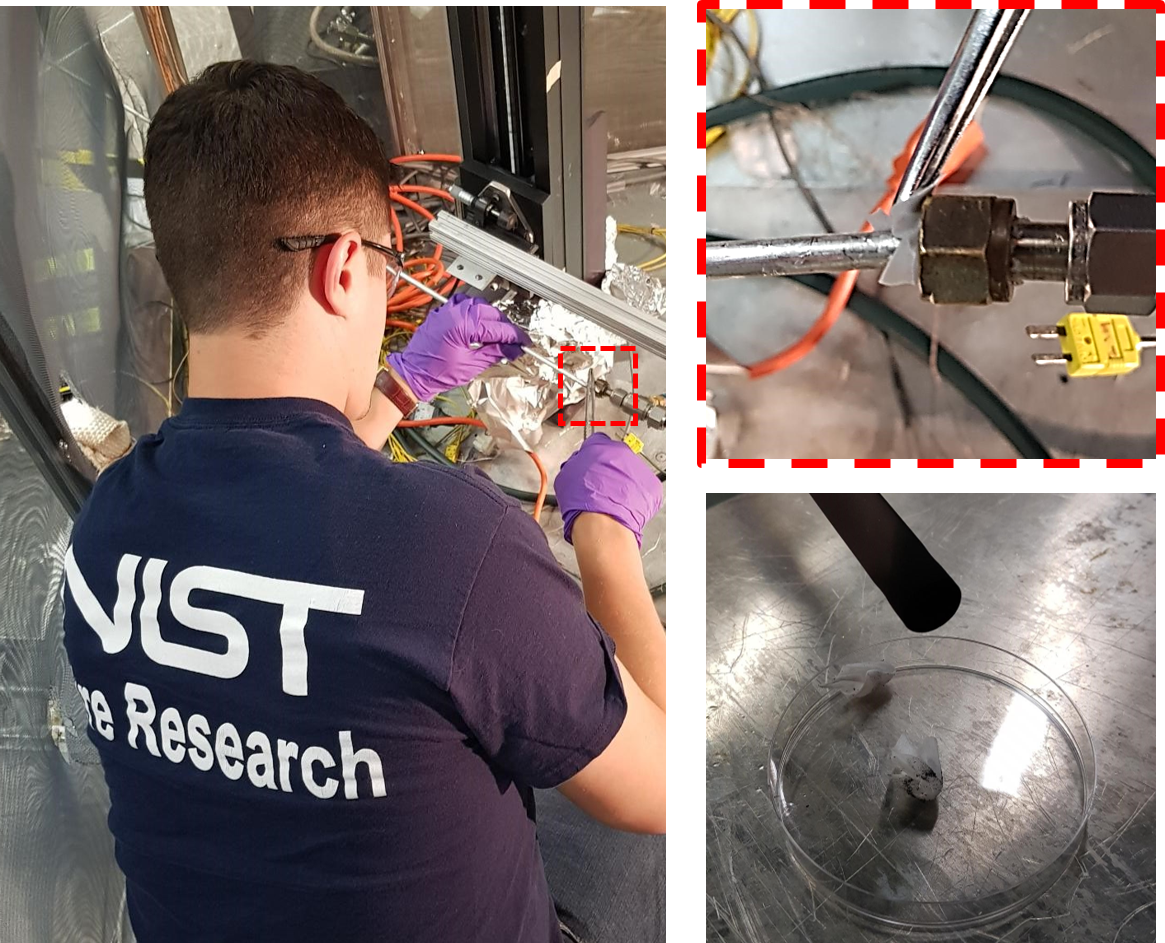
\includegraphics[width=15.0cm,keepaspectratio]{Soot_Probe.png}
	\caption[Process for cleaning soot probe]{Process of collecting soot from the internal walls of the quenching probe using gun cleaning patches}
	\label{fig:Soot_Probe_Setup}
\end{figure}

The soot mass fraction, $Y_{\rm s}$, is computed from the ratio of the mass of the soot collected from the PTFE filter and gun cleaning patches, $m_{\rm s}$, and the total mass of gas sampled, $m_{\rm tot}$, measured from the mass flow controller readings:
\begin{equation}\label{eq:soot_mass_frac}
Y_{s}= \frac{m_{\rm s}}{m_{\rm tot}}
\end{equation}
The total mass of gas sampled is the product of the average volumetric flow rate measured by the mass flow controller, $\dot{V}$, the density of the sample gas injected into the GC/MS, $\rho_{\rm gas}$, the gas sampling time, $\Delta t$, and the ratio of the mass flow controller's temperature reading, $T_{\infty}$, to the effective temperature of the gas calculated from Eq.~(\ref{eq:Thermocouple_Bead_Correction}), $T_{\rm g}$. 
\begin{equation}\label{eq:total_mass}
m_{t}= \dot{V} \, \rho_{gas}\, \Delta t \frac{T_{\infty}}{T_{\rm g}}
\end{equation}
In Eq.~(\ref{eq:total_mass}), the density of the sample gas is determined from the total mass detected from the TCD and MS, $m_{\rm tot}$, for the injected sample volume, $V_{\rm s}$.
\begin{equation}\label{eq:gas_density}
\rho_{\rm gas}= \frac{m_{\rm tot}}{V_{\rm s}}
\end{equation}
A description of the soot mass fraction uncertainty is provided in Appendix~\ref{sec:Uncertainty_Soot_Frac}.


\clearpage

\section{Results}
\label{sec:Results}

This section presents the flame height, temperature, gas species, and soot measurements made at incremental heights along the centerline of 30~cm diameter methanol, ethanol, and acetone pool fires and a \textcolor{red}{37~cm effective diameter methane and propane pool fires}.

\subsection{Flame Observations}
\label{ssec:Flame_Observations}

Figure~\ref{fig:Flame_Structure} displays a series of snapshots depicting a single pulsation cycle of the methanol, ethanol, and acetone fires. The pulsation frequency is approximately 3~Hz.
\begin{sidewaysfigure}[p]
	\centering
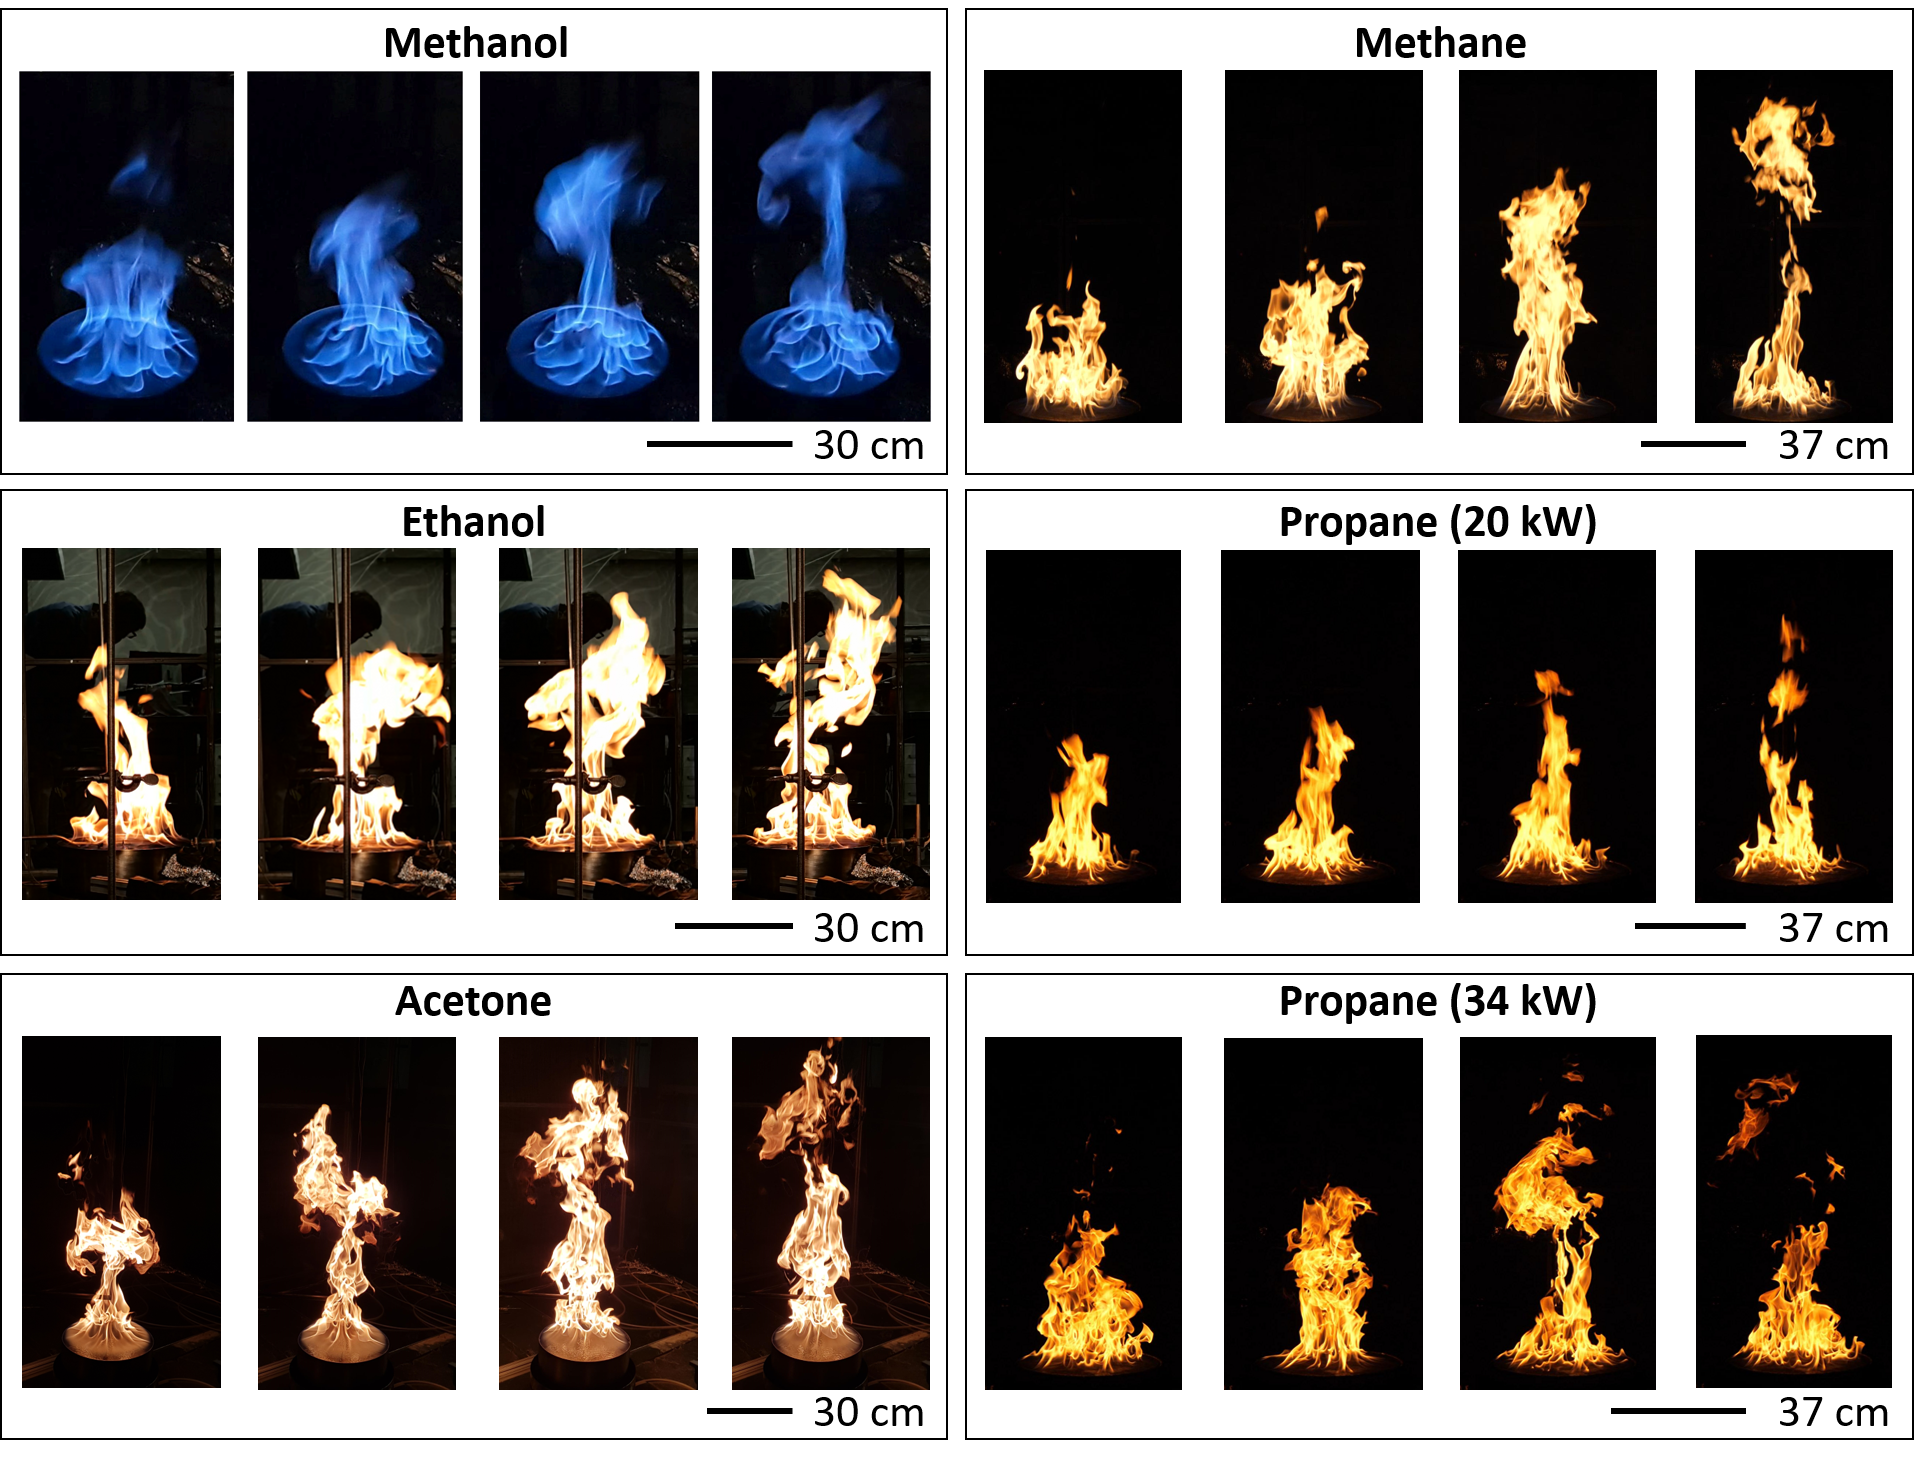
\includegraphics[width=\textwidth,keepaspectratio]{Flame_Structure.png}
	\caption[Photographs of the three fires]{Flame structures of methanol, ethanol, acetone, methane, and propane pool fires during their pulsing cycles}
	\label{fig:Flame_Structure}
\end{sidewaysfigure}
The methanol fire is purely blue, whereas the ethanol, acetone, methane, and propane fires are more luminous and yellow. The measured time-averaged burning rates and calculated heat release rates are listed in Table~\ref{tab:Pool_Fire_Parameters_Table}. The heat release rates are calculated from Eq.~(\ref{eq:Heat_release_rate}).The methanol fire has the lowest average flame height, followed by the propane, ethanol, methane, and acetone. The measured mean flame heights match Heskestad’s correlation~\cite{Heskestad1983} to within measurement uncertainty. The measured flame heights are also within the uncertainty bounds of measurements made by Kim~et~al.~\cite{Kim2019}. 
\begin{equation}
\frac{L_{\rm f}}{D} = 3.7 \, (\dot{Q}^*)^{2/5} - 1.02 \quad ; \quad \dot{Q}^*=\frac{\dot{Q}}{c_{p}\rho_\infty T_\infty \sqrt{g} \, D^{5/2}}
\end{equation}
Here, $D$ is the diameter of the pool fire (30~cm), $g$ is the acceleration of gravity, and $c_p$ and $\rho_\infty$ are the specific heat and the density of air at room temperature, $T_\infty$. The measured flame heights are also within the uncertainty bounds of measurements made by Kim~et~al.~\cite{Kim2019}.

\begin{table}[!t]
\caption[List of measurements and thermochemical properties of fuels]{List of measurements and thermochemical properties of fuels burning in a well-ventilated round 30~cm diameter and a 37~cm diameter pool fire burning in a quiescent environment. The uncertainty of the mass burning rate is discussed in Appendix~\ref{ssec:Mass_Burning_Flux}. The uncertainty of the heat release rate and $\dot{Q}^*$ is discussed in Appendix~\ref{ssec:Heat_Release_Rate}.}
\label{tab:Pool_Fire_Parameters_Table}
\centering
	\footnotesize
	\begin{tabular}{p{0.125\linewidth}p{0.1\linewidth}p{0.1\linewidth}p{0.1\linewidth}p{0.1\linewidth}p{0.1\linewidth}p{0.1\linewidth}}
\hline
%\\[0.0005cm]
\textbf{Parameter (units)} &\textbf{Methanol}& \textbf{Ethanol}& \textbf{Acetone}&\textbf{Methane}&\textbf{Propane}&\textbf{Propane}\\
\hline
\\[0.01cm]
Mass Burning Flux~(\si{g/{m^2 s}})	&	12.4~$\pm$~1.1		&	13.9~$\pm$~0.8		&	17.6~$\pm$~2.7		&	6.4~$\pm$~0.1	&4.2~$\pm$~0.1		& 6.9~$\pm$~0.1\\
\\[0.01cm]
Heat Release Rate~(\si{kW})		&	17.4~$\pm$~1.4		&	26.3~$\pm$~1.5		&	35.5~$\pm$~5.4		&	34.5~$\pm$~0.5	&20.7~$\pm$~0.6  	& 34.4~$\pm$~0.6\\
\\[0.01cm]							
$\dot{Q}^* $				&	0.32~$\pm$~0.02		&	0.48~$\pm$~0.01		&	0.64~$\pm$~0.05		&	0.37~$\pm$~0.01	&0.22~$\pm$~0.01	& 0.37~$\pm$~0.01\\	
\\[0.01cm]
$D^*$~(\si{m})				&	0.19~$\pm$~0.01		&	0.22~$\pm$~0.01		&	0.25~$\pm$~0.02		& 	0.25~$\pm$~0.01	&0.20~$\pm$~0.01 	& 0.25~$\pm$~0.01\\
\\[0.01cm]
Mean Flame Height~(\si{cm})		&	36.4~$\pm$~16.0		&	61.1~$\pm$~28.2		&	91.5~$\pm$~34.6		&	64.0~$\pm$~31.0	&	38.3~$\pm$~14.6	& 50.0~$\pm$~16.0\\
\\[0.01cm]
Heat of Combustion (kJ/g)~\cite{SFPE}	&	19.94				&	26.81				&	28.56				&	50.03			&	46.34			& 46.34	\\	
\\[0.01cm]
C/H Ratio					&	1/4				&	1/3				&	1/2				&	1/4			&	3/8			& 3/8\\
\hline
\end{tabular}
\end{table}

\subsection{Comparison of Pool Fires from Different Fuels}
\label{ssec:Fuel_comp}

Figure~\ref{fig:Temp_Comparison} displays the time-averaged, corrected gas temperatures as a function of the normalized vertical spatial coordinate, $z^*$:
\begin{equation}\label{eq:Z_Star}
z^*=\frac{z}{D^*}  \quad ; \quad  D^* = \left(\frac{\dot{Q}}{c_{p}\rho_\infty T_\infty \sqrt{g}}\right)^{\frac{2}{5}}
\end{equation}
Here, $z$ is the vertical spatial coordinate, $\dot{Q}$ is the heat release rate, $g$ is the acceleration of gravity, and $c_p$ and $\rho_\infty$ are the specific heat and the density of air at room temperature, $T_\infty$. The maximum mean temperature for each fuel peaks at approximately $z^*=0.2$. The maximum mean temperature for each fuel peaks is close to their respective stoichiometric mixture fraction values. The methanol temperature profile is in agreement with previous works~\cite{Wang2019}. The thermal inertia correction applied to the thermocouple temperature has less than a 5~K influence on the mean but significantly alters the RMS. 

\begin{figure}[h!]
	\centering
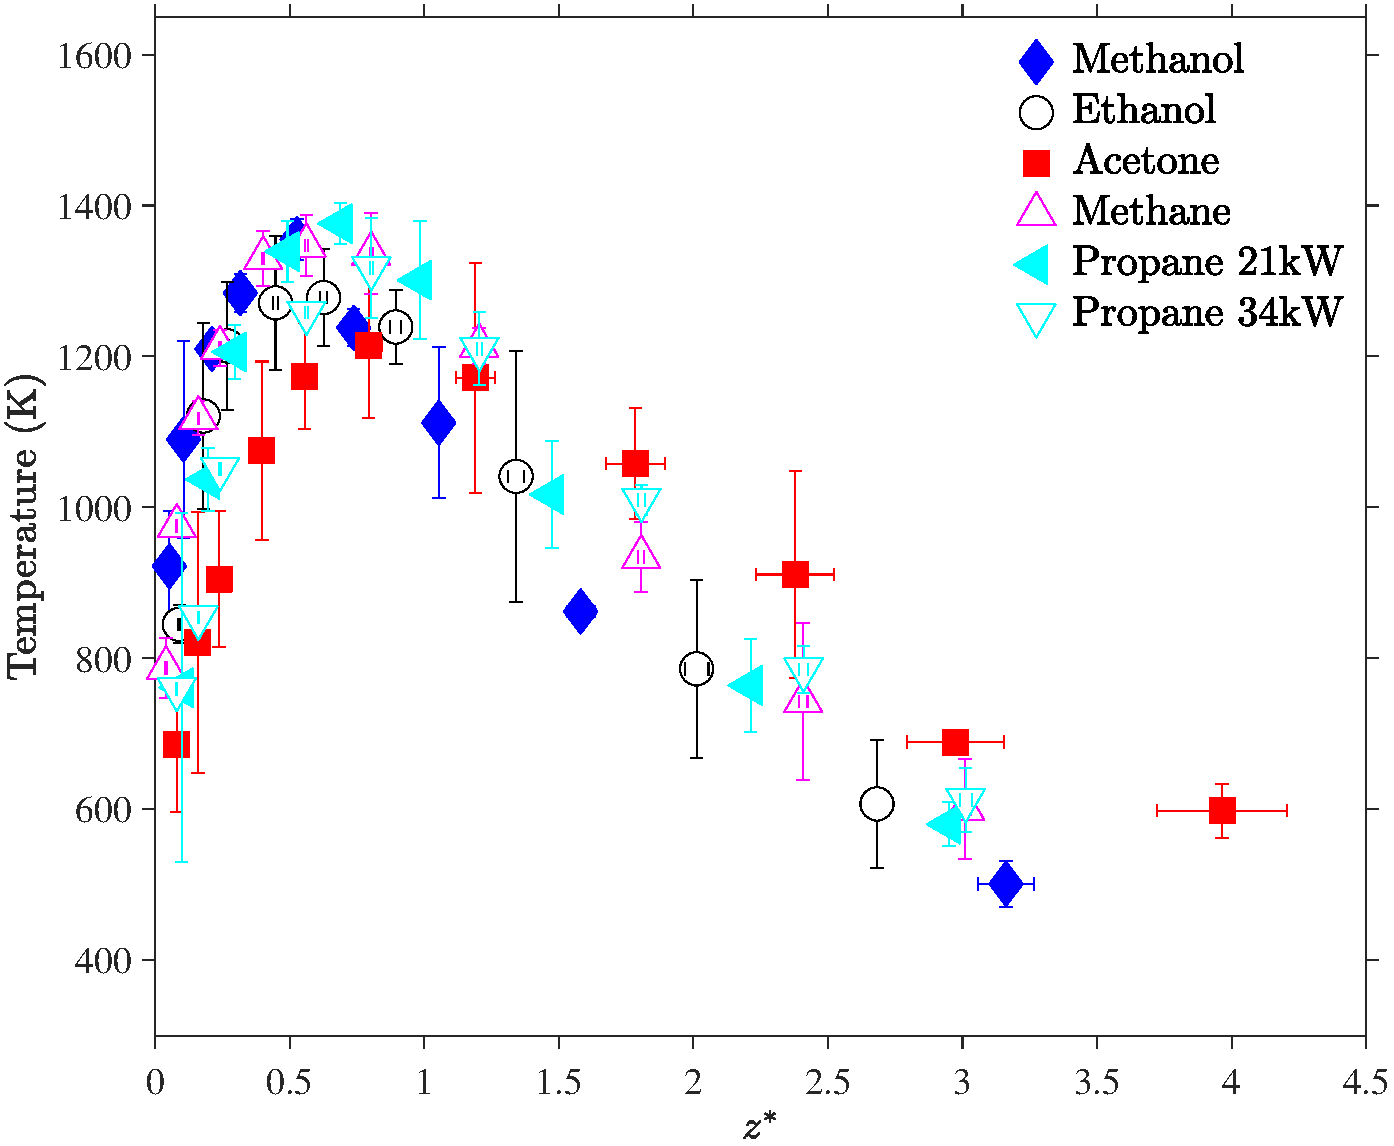
\includegraphics[width=10.0 cm, keepaspectratio]{Temperature_Comparison.pdf}
	\caption[Mean and RMS centerline gas temperature profiles]{Mean and root mean square (RMS) centerline gas temperature profiles of methanol, ethanol, acetone, methane\textcolor{red}{, and propane} pool fires during their pulsing cycles \textcolor{red}{ as a function of $z^*$}}
	\label{fig:Temp_Comparison}
\end{figure}

\textcolor{red}{Figure \ref{fig:Vel_Comparison} shows the mean and standard deviation of the upward gas velocity along the pool centerline as a function of $z^*$ (based on axial distance above the fuel surface) in the 30 cm diameter liquid pool fires and the 37~cm effective diameter gaseous pool fires. The results reported here complement those of Weckman~\cite{Weckman1996}, extending the measurement range from 1 one diameter above the fuel surface to about 4 times the burner diameter.  The upward velocity along the centerline monotonically accelerates for about the first diameter above the fuel surface.  After one diameter, the upward velocity plateaus and slowly decreases with distance above the burner surface.    The velocity profiles are similar. The methanol fire has the smallest peak velocity, whereas the others are similar.}


\begin{figure}[h!]
	\centering
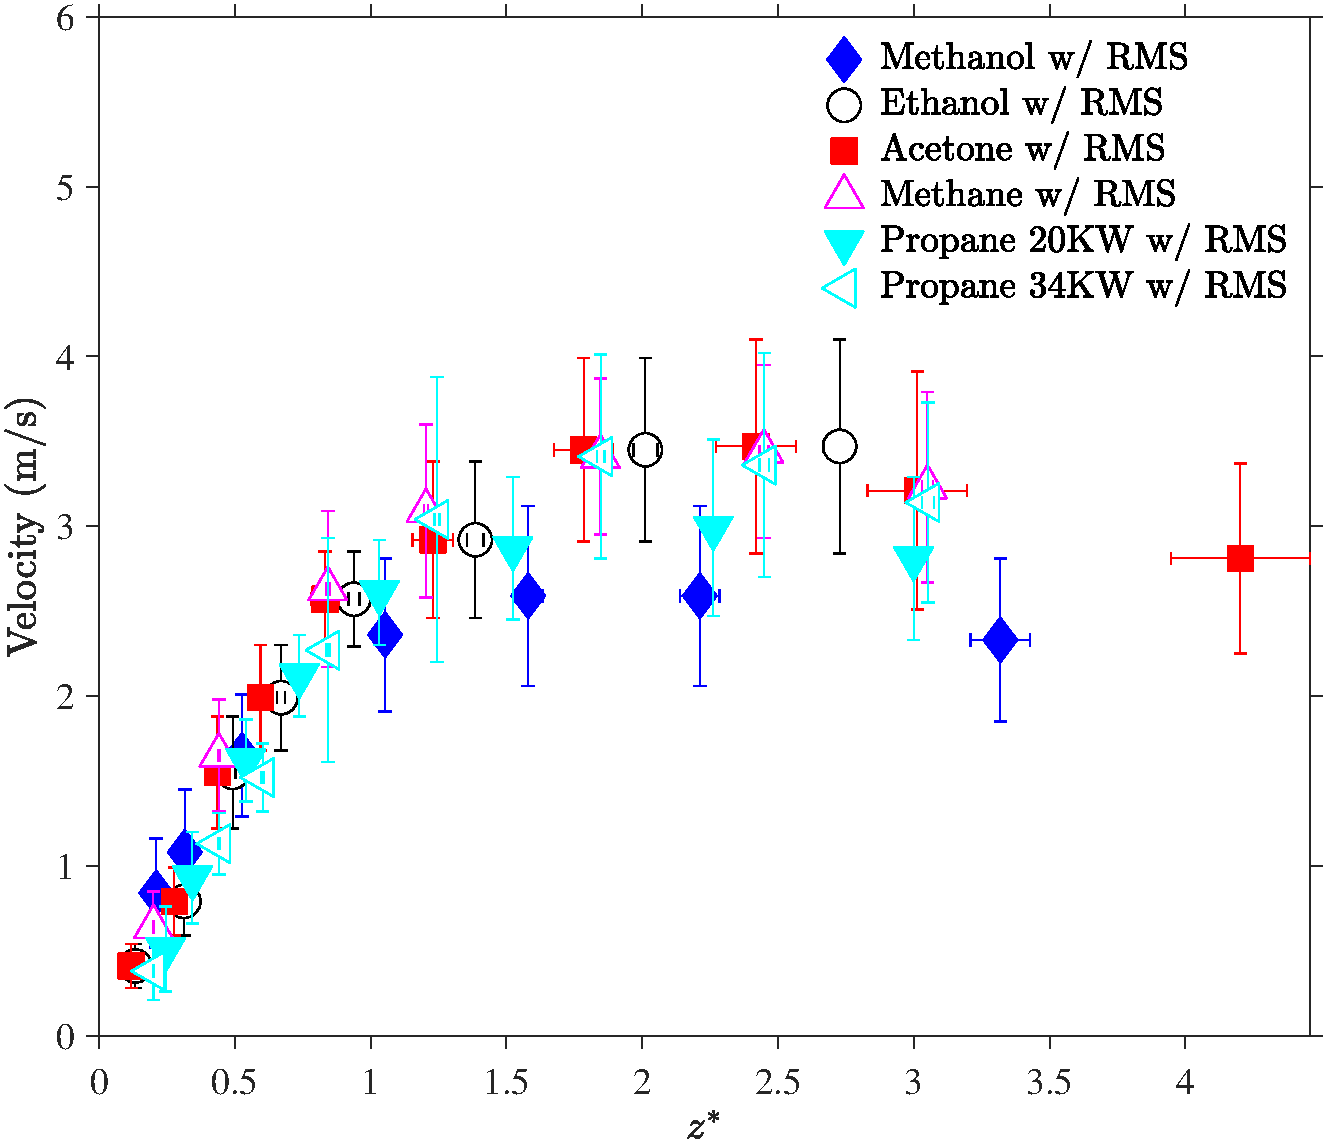
\includegraphics[width=10.0 cm, keepaspectratio]{Velocity_Comparison.pdf}
	\caption[Mean and RMS centerline velocity profiles]{Mean and root mean square (RMS) centerline velocity profiles of methanol, ethanol, acetone, methane\textcolor{red}{, and propane} pool fires during their pulsing cycles \textcolor{red}{ as a function of $z^*$}}
	\label{fig:Vel_Comparison}
\end{figure}

Figure~\ref{fig:Fuel_Comparison} displays the mean volume fraction of the major species, $\bar{X}_{i}$, as a function of $z^*$ for the methanol, ethanol, acetone, methane, and propane fires. Plots for individual species, including uncertainties, are displayed in Appendix~\ref{sec:Vol_Frac_Figs}. Major species detected in the TCD and MS include combustion reactants (fuels and oxygen, $\ch{O_2}$), combustion products such as water, $\ch{H_{2}O}$, and carbon dioxide, $\ch{CO_{2}}$, combustion intermediates such as carbon monoxide, $\ch{CO}$, hydrogen, $\ch{H_{2}}$, and inert gases such as nitrogen, $\ch{N_{2}}$, and argon, $\ch{Ar}$. Methane is detected and quantified in all fires. In the case of the ethanol and acetone fires, soot, benzene, acetylene, ethylene, and ethane are also detected and quantified. Trace amounts of other species are also detected including propene, acetaldehyde, and ethyl acetate, consistent with previous literature~\cite{Pichon2009, Gong2015}.

\begin{figure}[!]
	\centering
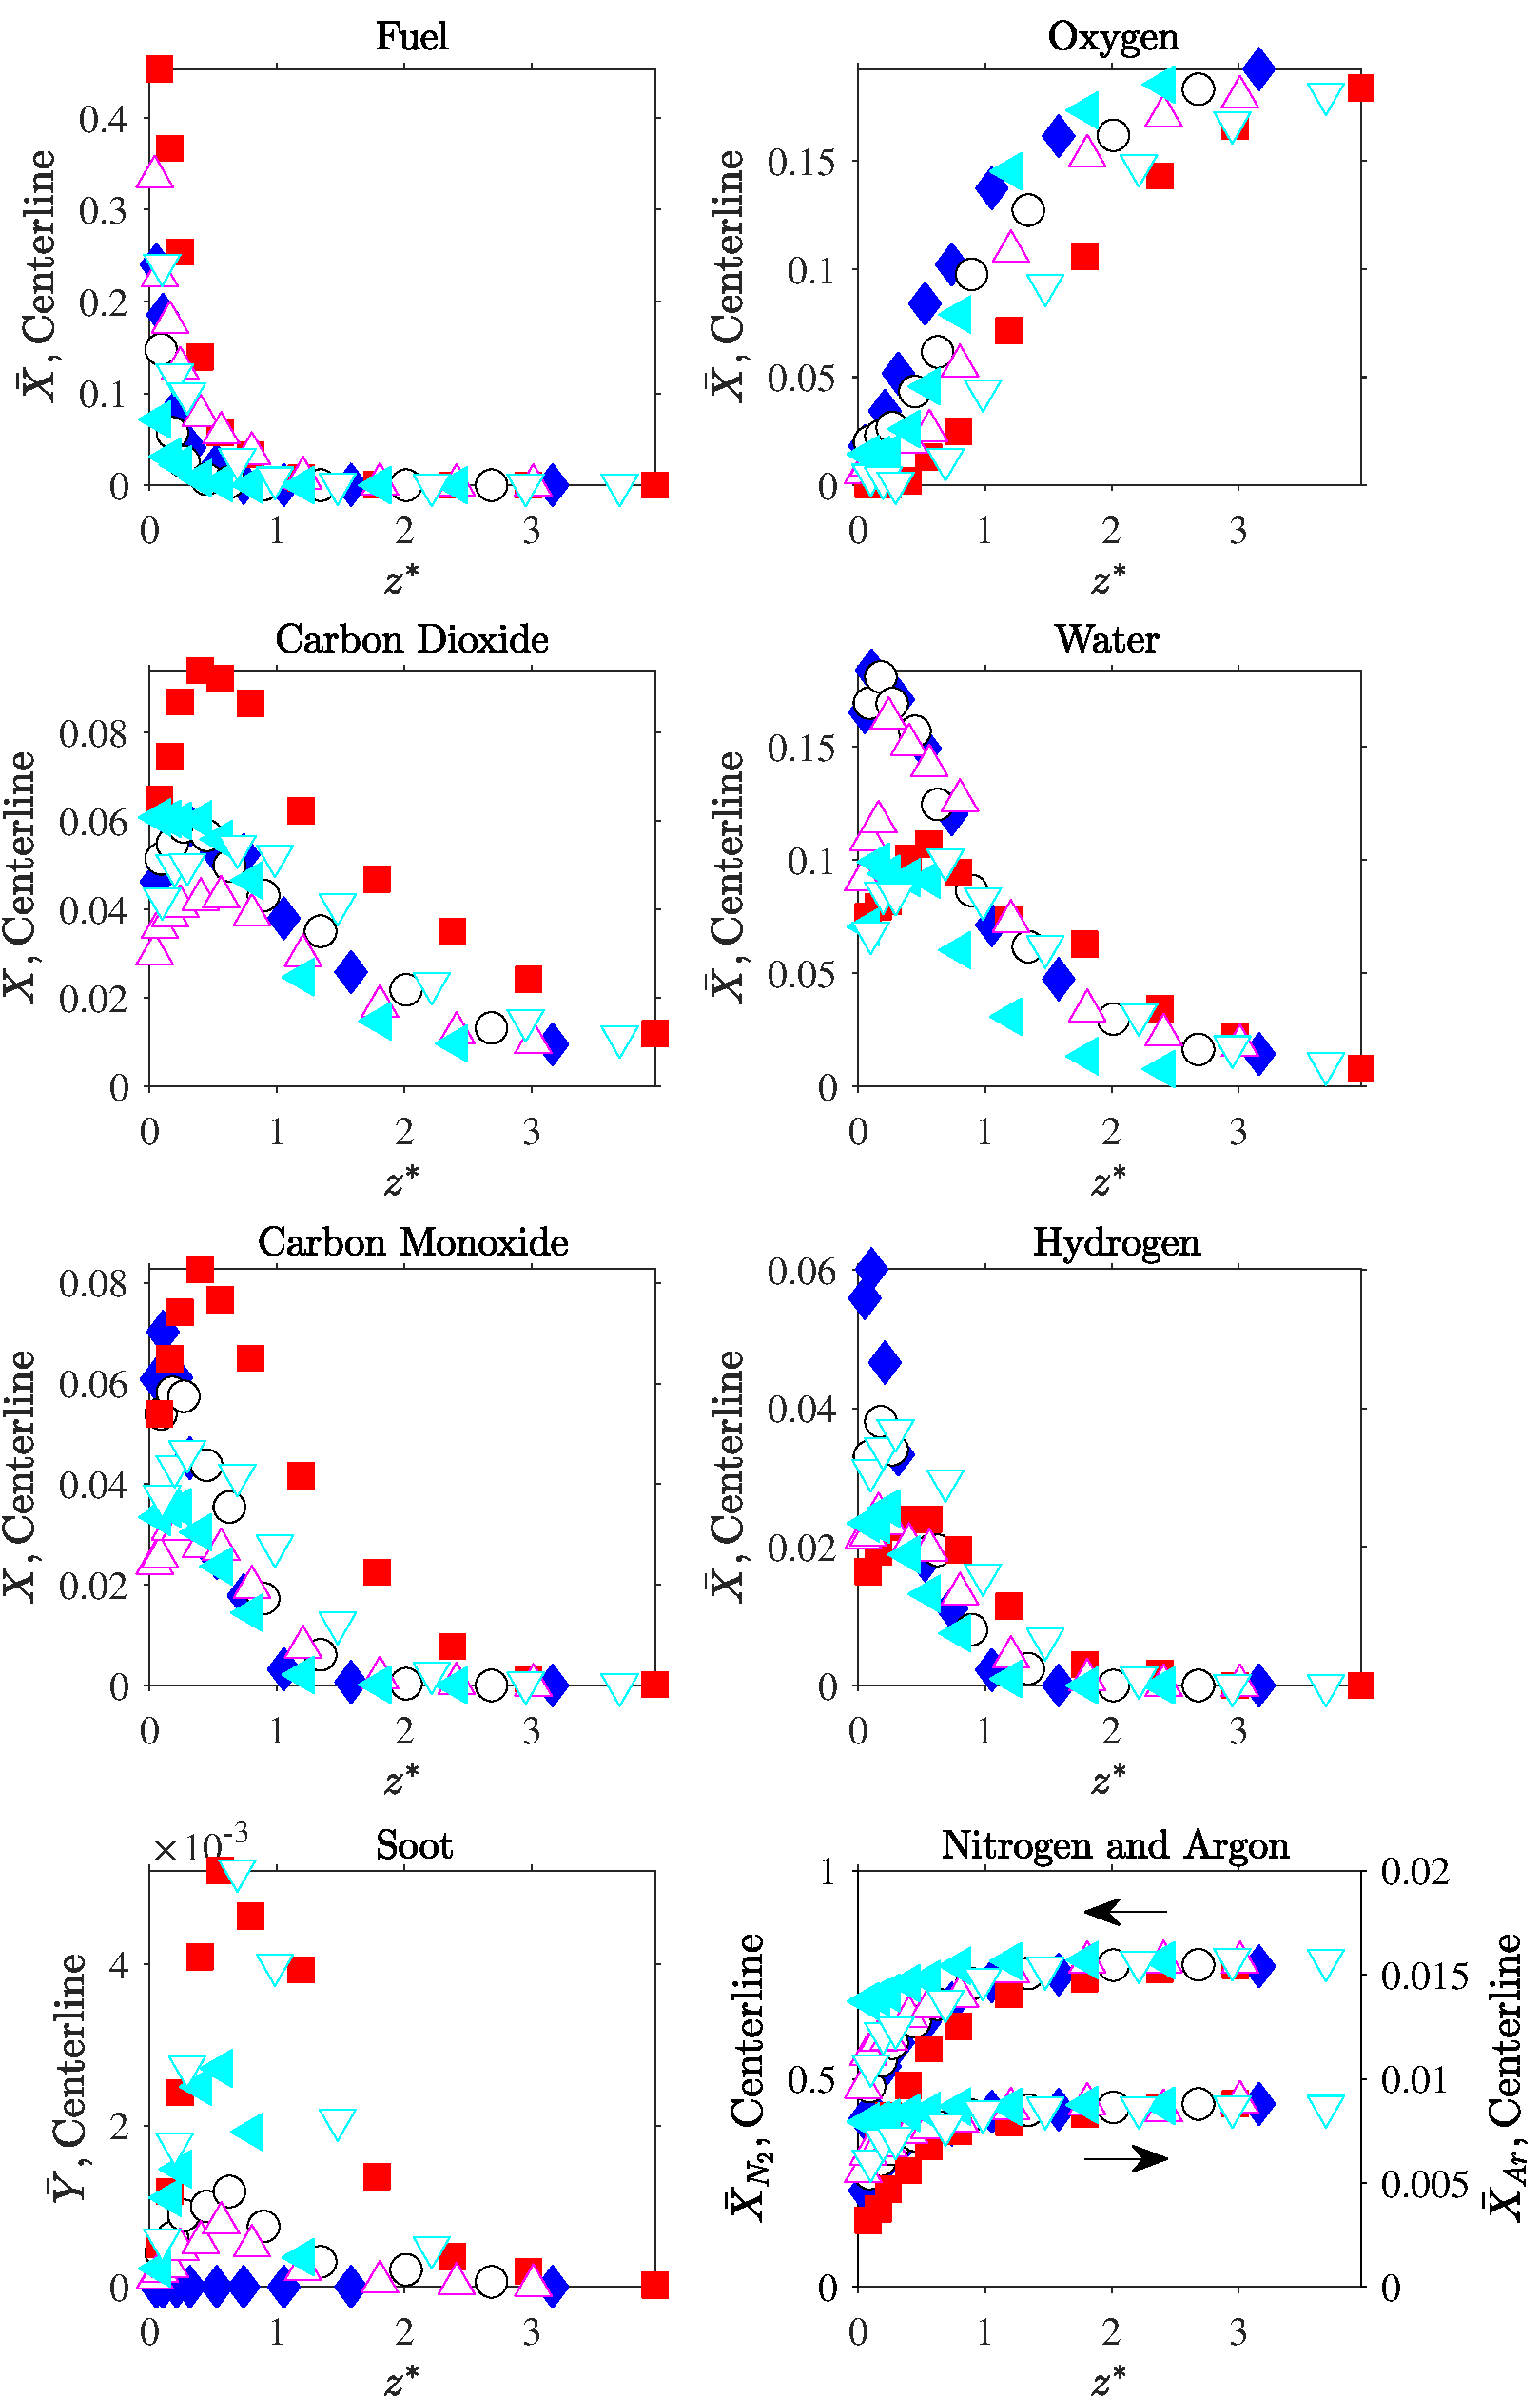
\includegraphics[width=12.5cm,keepaspectratio]{OVERALL_Fuel_Comparison.pdf}
	\caption[Centerline volume fraction and soot mass fraction profiles]{Centerline volume fraction and soot mass fraction profiles of methanol ($\blacklozenge$), ethanol ($\bigcirc$), acetone ($\blacksquare$), methane ($\triangle$), 20 kW propane ($\blacktriangleleft$), and 34 kW propane ($\bigtriangledown$) pool fires \textcolor{red}{ as a function of $z^*$}.}
	\label{fig:Fuel_Comparison}
\end{figure}


\clearpage

\section{Verifying Gas Species Measurements}
\label{ssec:Verifying_Vol_Frac_Measurements}

This section presents several different techniques of verifying the accuracy of the species concentration measurements.


\subsection{Counting Moles}

As a way to verify the accuracy of the experimental method, specifically the calibration procedure and curve fit, the total moles, $n_{\rm tot}$, identified by the TCD and MS is compared to the total moles injected into the GC/MS system, $n_{\rm inj}$, which is calculated from the ideal gas law:
\begin{equation}\label{eq:moles_inj}
n_{\rm inj}=\frac{PV_{\rm s}}{RT}
\end{equation}
Here, $R=8.314$~J/(mol$\cdot$K) is the universal gas constant, $V_{\rm s}=2\times 10^{-6}$~m$^3$ is the injected sample volume, and $P$~(Pa) and $T$~(K) are the mean pressure and temperature, respectively, collected before injecting the gas sample into the GC/MS as described in Section~\ref{ssec:Gas_Species_Setup}. The combined uncertainty of the total moles injected is detailed in Section~\ref{ssec:Total Moles Injected into the GC/MS for Calibation}.

\begin{figure}[h!]
	\centering
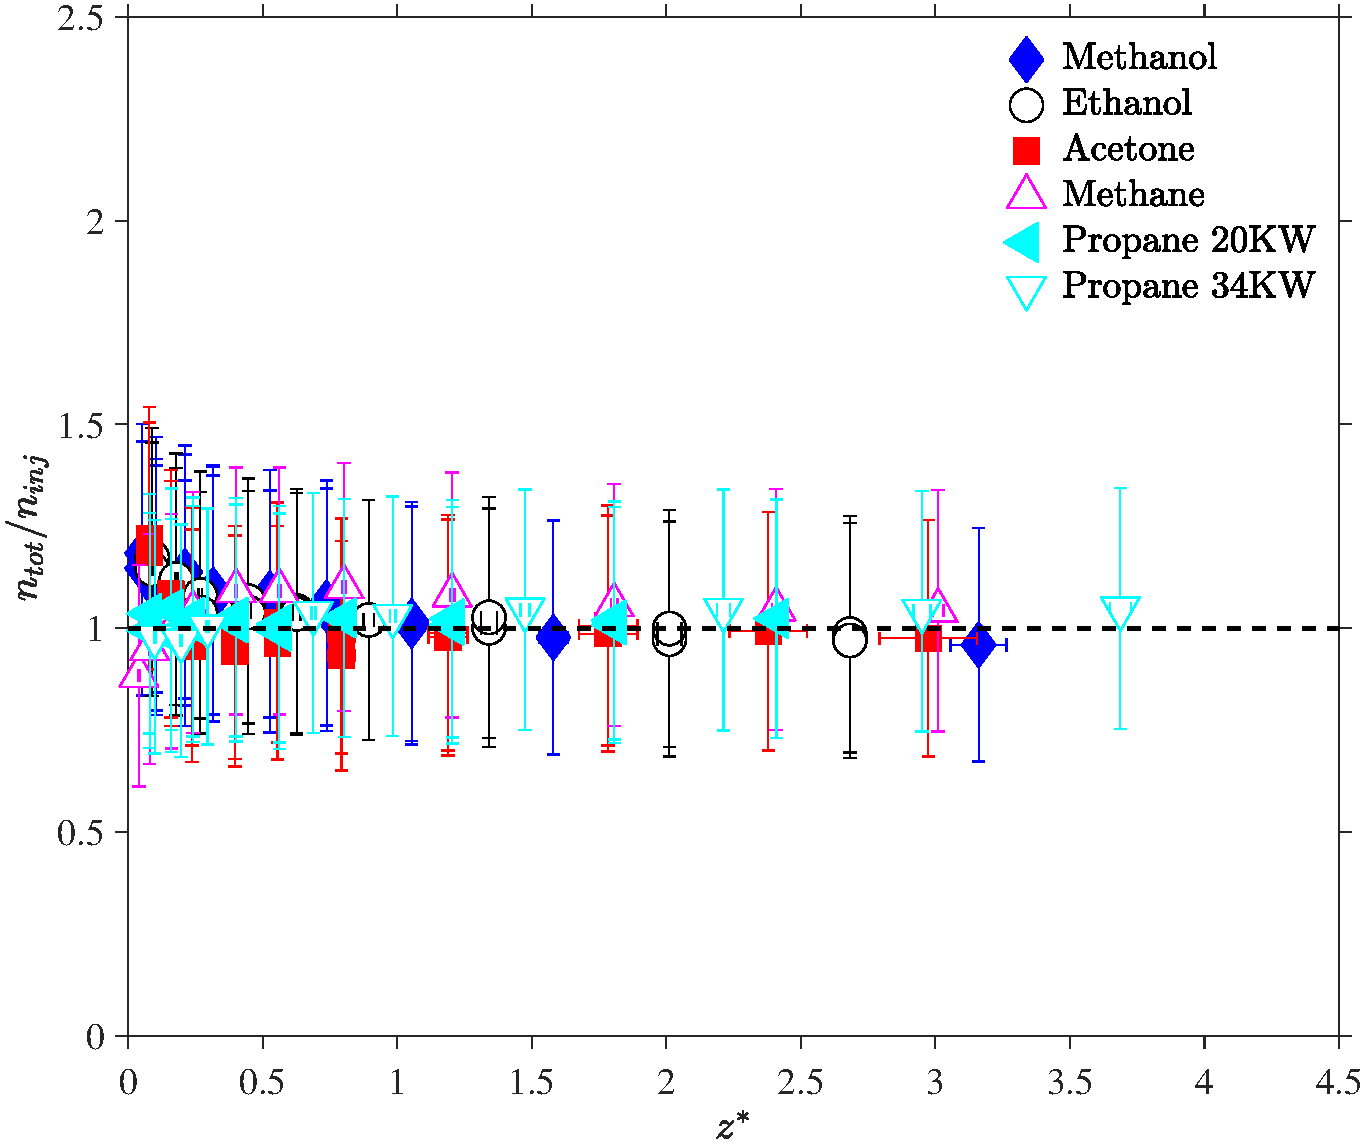
\includegraphics[width=10.0cm,keepaspectratio]{mole_ratio_Comparison.pdf}
	\caption[Ratio of moles identified to moles injected]{Ratio of moles identified to moles injected, with uncertainty, as a function of $z^*$. The uncertainty of the ratio is defined in in Section~\ref{ssec:mole ratio}.}
	\label{fig:Mole_Comp}
\end{figure}

Figure~\ref{fig:Mole_Comp} shows the ratio of the moles identified by the TCD and MS to the mole injected into the GC/MS as a function of $z^*$. In most cases, the ratio is close to unity, indicating that the total moles injected into the GC/MS are all accounted for in the calculation. For low values of $z^*$, the ratio is higher than unity, indicating an error in the calibration which is most likely due to an over-prediction of the fuel species that are found at high concentrations near the fuel surface. \textcolor{red}{In comparison, the expected values and estimated results are consistent within the experimental uncertainty, validating the calibration process of all detected species.}

\subsection{Carbon to Hydrogen Ratio}

Another way to verify the accuracy of the gas species measurements is to calculate the ratio of carbon to hydrogen atoms contained in all gas species at each vertical measurement location:
\begin{equation}\label{eq:c2h_ratio}
  \frac{\rm C}{\rm H}= \frac{\textrm{W}_{\rm{C}}}{\textrm{W}_{\rm{H}}}\, \frac{ \sum  {\rm x}_i \, \bar{X}_{i}}{\sum {\rm y}_i \, \bar{X}_{i}}
\end{equation}
where the summation is over all measured gas species, and ${\rm x}_i$ and ${\rm y}_i$ are the numbers of carbon and hydrogen atoms in the molecule, respectively. The carbon to hydrogen ratio of the fuel molecules are reported in Table~\ref{tab:Pool_Fire_Parameters_Table}, and the ratio for each fuel is shown in Fig.~\ref{fig:C2H}.

\begin{figure}[h!]
	\centering
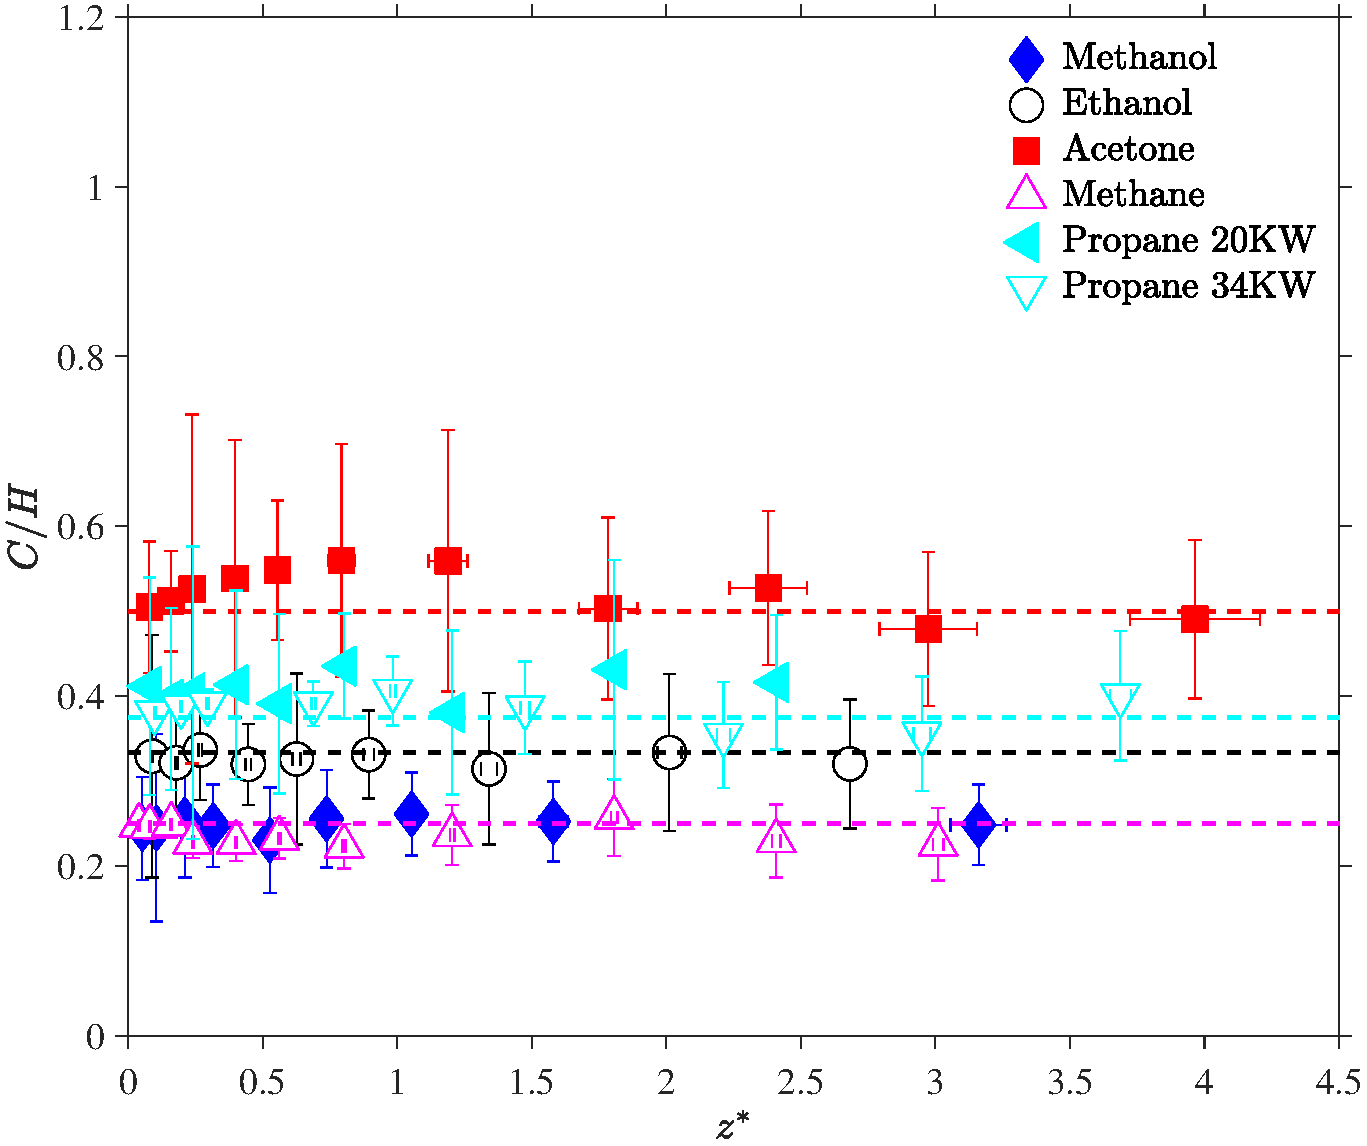
\includegraphics[width=10.0cm, keepaspectratio]{C2H_ratio_Comparison.pdf}
	\caption[Carbon to hydrogen ratio calculated from all species]{Carbon to hydrogen ratio calculated from all measured gas species compared to the theoretical values \textcolor{red}{ as a function of $z^*$}.The uncertainty of the ratio is defined in in Section~\ref{ssec:C2H_ratio}.}
	\label{fig:C2H}
\end{figure}

\textcolor{red}{Figure~\ref{fig:C2H} shows the comparison between the hydrogen to carbon ratio of the parent fuel, indicated by the dotted lines, and the calculated ratio at various positions within the centerline of the fires. In all cases, the calculated {C}\textbackslash{H} is within the experimental uncertainty of the parent fuels' ratios. In several cases, the expected and calculated values are nearly matching, indicating that the concentration measurements of species that consist of carbon and hydrogen are accurately estimated using the experimental method. The consistency of the {C}/{H} at different positions along the centerline of the fires also suggests that each of the extracted gas samples are well-mixed, as expected, showing no uneven distribution of carbon or hydrogen atoms when measured throughout the fire.}

Another verification test considers the inert species argon and nitrogen whose molar ratio should be the same regardless of fuel type. The measured Ar/N$_2$ ratio in ambient air is $0.0117\pm0.0005$, and the measured ratio at different vertical locations within the fires is depicted in Fig.~\ref{fig:IR}. All points fall within the uncertainty bounds of the ambient air measurement\textcolor{red}{, indicating that measurements of the concentrations of argon and nitrogen are reasonable throughout the fire. Similarly to the {C}/{H}, the consistency of the inert gas ratio suggests the extracted sample is well-mixed, further supporting the validity of the experimental methods.}
 
\begin{figure}[h!]
	\centering
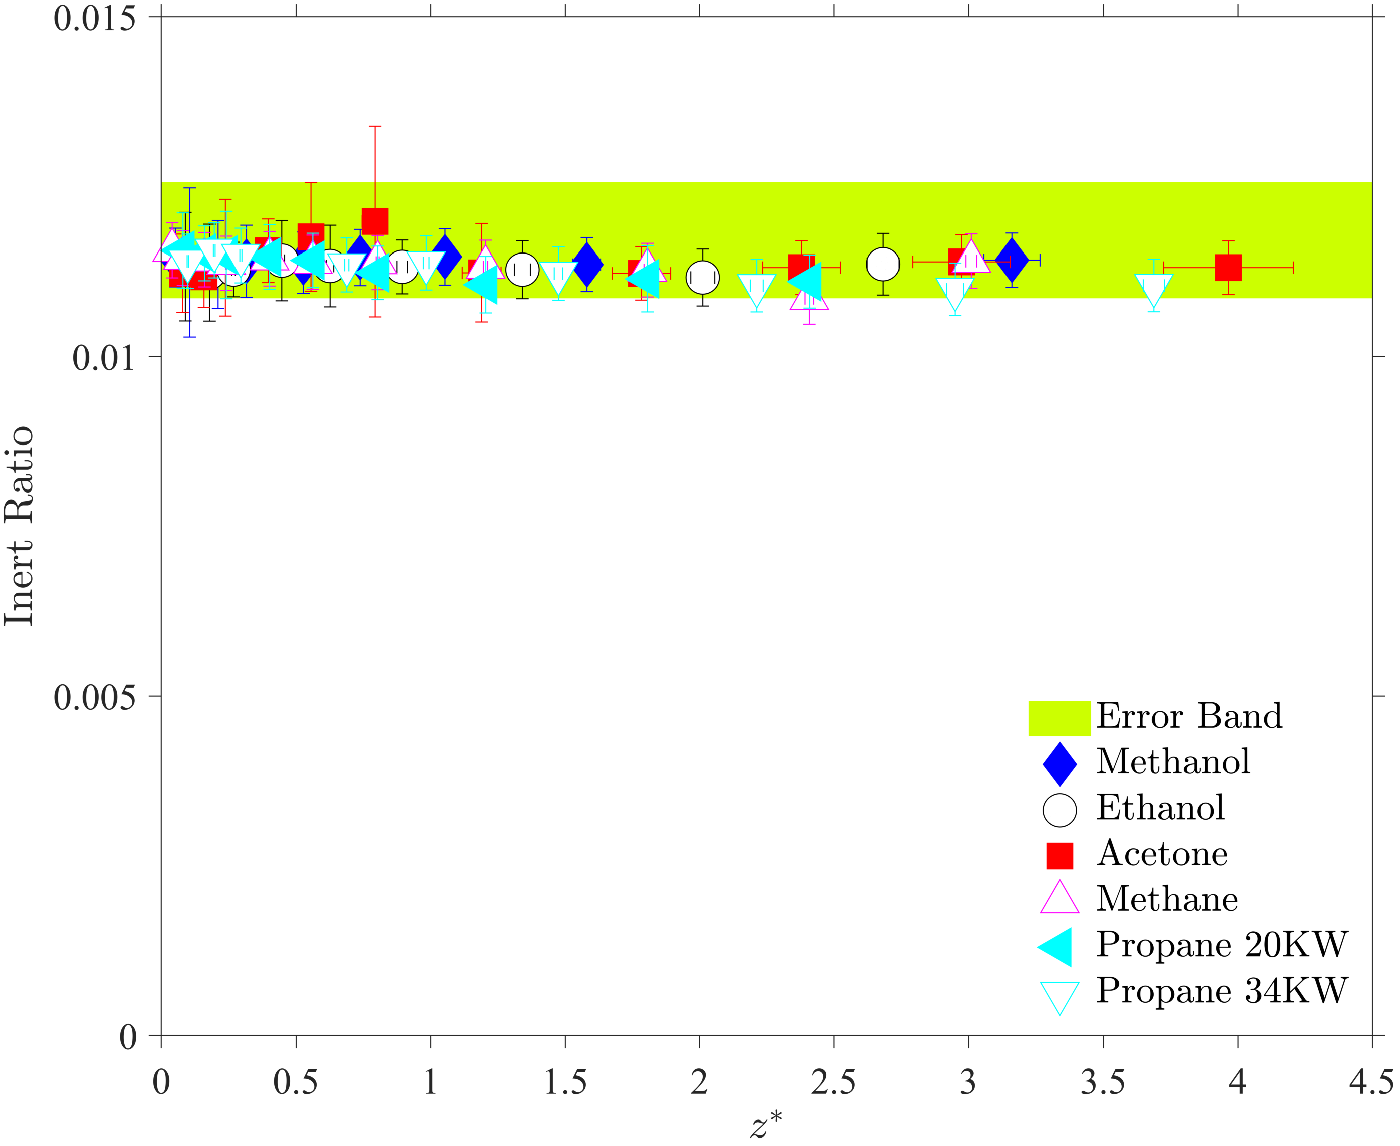
\includegraphics[width=10.0cm, keepaspectratio]{Inert_ratio_Comparison.pdf}
	\caption[Ar/N$_2$ ratio within the fire envelop compared to ambient air]{Ar/N$_2$ molar ratio at different elevations compared to the uncertainty bounds of the measurement in ambient air \textcolor{red}{ as a function of $z^*$}.The uncertainty of the ratio is defined in in Section~\ref{ssec:Inert_ratio}.}
	\label{fig:IR}
\end{figure}
\clearpage


\subsection{Plotting the Results in Mixture Fraction Space}
\label{ssec:Mixture_Fraction_Results}

The mixture fraction, $Z$, is defined as the mass fraction of the gases containing carbon, in addition to soot, that originate in the fuel stream. It can be expressed\footnote{The uncertainty of the mixture fraction is determined from propagating the error in the mass fraction measurements. A detailed description of the mixture fraction uncertainty is provided in Appendix~\ref{sec:Uncertainty_Mix_Frac}.} as follows:
\begin{equation}\label{eq:Mixture_Fraction}
  Z = \bar{Y}_{\rm F} + \frac{W_{\rm F}}{\rm x} \sum_{i\ne {\rm F}} \frac{\bar{Y}_i}{W_{i}}
\end{equation}
where $\bar{Y}_{\rm F}$, ${W_{\rm F}}$, and $\rm x$ are the mass fraction, molecular weight, and number of carbon atoms in the fuel molecule, respectively. Assuming ideal (i.e. no CO or soot), infinitely-fast (fuel and oxygen from the air cannot co-exist) combustion, the mass fractions of all species can be expressed as piece-wise linear ``state relations'' according to the following reaction:
\begin{align*}
{\rm C}_{\rm x}{\rm H}_{\rm y}{\rm O}_{\rm z} & +\eta(\rm x+\frac{\rm y}{4}-\frac{\rm z}{2})~({\rm O}_{2}+3.76~{\rm N}_{2}+0.0445~{\rm Ar}) \rightarrow  \\
          & \max(0,1-\eta)~{\rm C}_{\rm x}{\rm H}_{\rm y}{\rm O}_{\rm z}+\max(0,1-\eta)~(\rm x+\frac{\rm y}{4}-\frac{\rm z}{2})~{\rm O}_{2}+ \min(1,\eta)~\rm x~{\rm CO}_{2} +  \\
          & \min(1,\eta)~\frac{\rm y}{2}~{\rm H}_{2}{\rm O}+\eta(\rm x+\frac{\rm y}{4}-\frac{\rm z}{2})~(3.76~{\rm N}_{2}+0.0445~{\rm Ar})  \numberthis \label{eq:Ideal_rxn}
\end{align*}
The parameter $\eta$ is the reciprocal of the local fuel equivalence ratio, $\phi$,
\begin{equation}\label{eq:Eta}
\phi=\frac{\rm (F/A)}{{\rm (F/A)}_{\rm st}}=\frac{1}{\eta}
\end{equation}
where $\rm F/A$ is the fuel-air mass ratio and the subscript $\rm st$ denotes the stoichiometric condition.

Figures~\ref{fig:Methanol_Mix_Frac}, \ref{fig:Ethanol_Mix_Frac}, \ref{fig:Acetone_Mix_Frac}, \ref{fig:Methane_Mix_Frac}, \ref{fig:Propane20kW_Mix_Frac}, and \ref{fig:Propane34kW_Mix_Frac} show the mean mass fraction measurements as a function of the mixture fraction for the methanol, ethanol, acetone, methane, and propane fires, respectively. The dotted lines represent ideal combustion calculated from Eq.~(\ref{eq:Ideal_rxn}). The vertical dotted line identifies the stoichiometric value of the mixture fraction. Additional plots that detail the averaged mass fractions of all detected species as a function of mixture fraction, with their expanded uncertainties, are provided in Appendix~\ref{sec:Mix_Frac_Figs}.

\begin{figure}[!]
	\centering
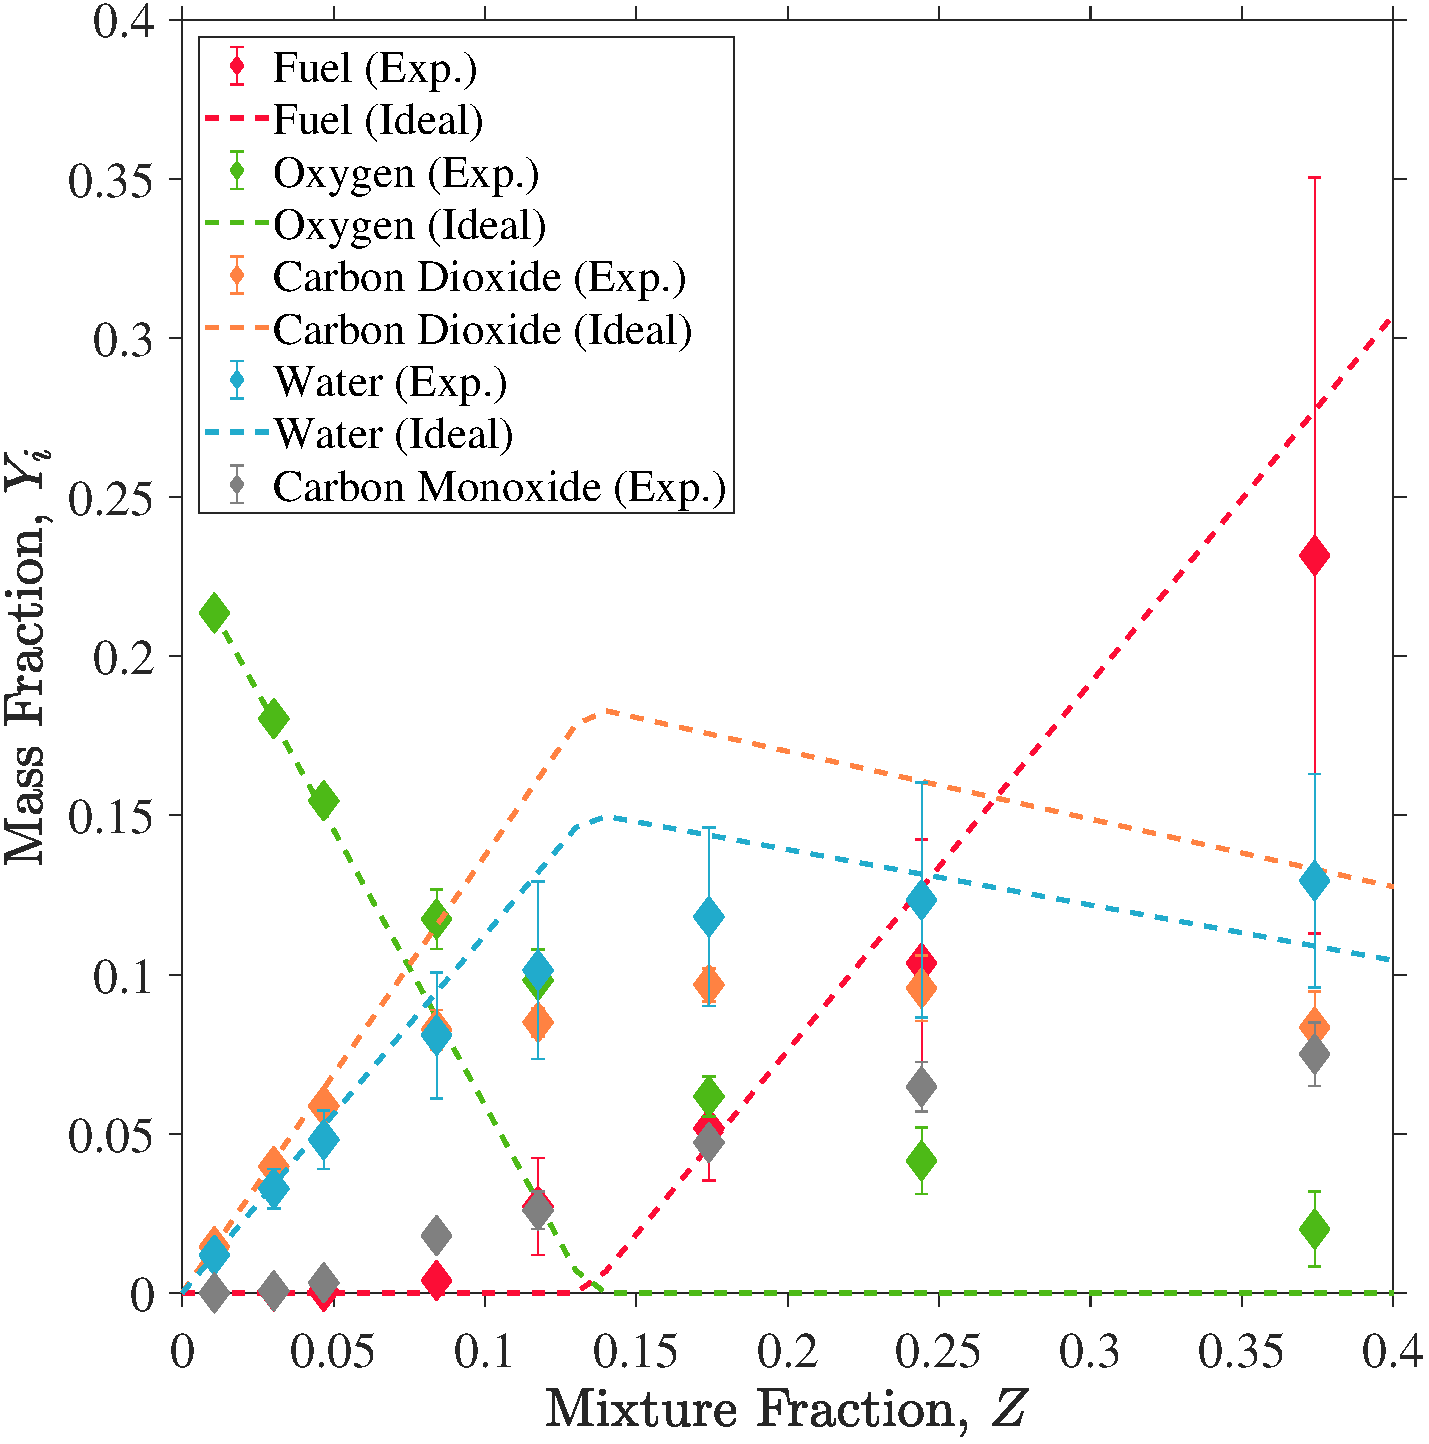
\includegraphics[width=\textwidth,keepaspectratio]{Adjusted_FuelMethanol_Mixture_Fraction_Intermediate_Plot.pdf}
	\caption[Mean mass fractions as a function of mixture fraction, methanol]{Mean mass fractions as a function of mixture fraction, methanol. The uncertainty of the mean mass fractions shown here is defined in Section~\ref{ssec:Uncertainty of Mass Fractions}.}
	\label{fig:Methanol_Mix_Frac}
\end{figure}

\begin{figure}[!]
	\centering
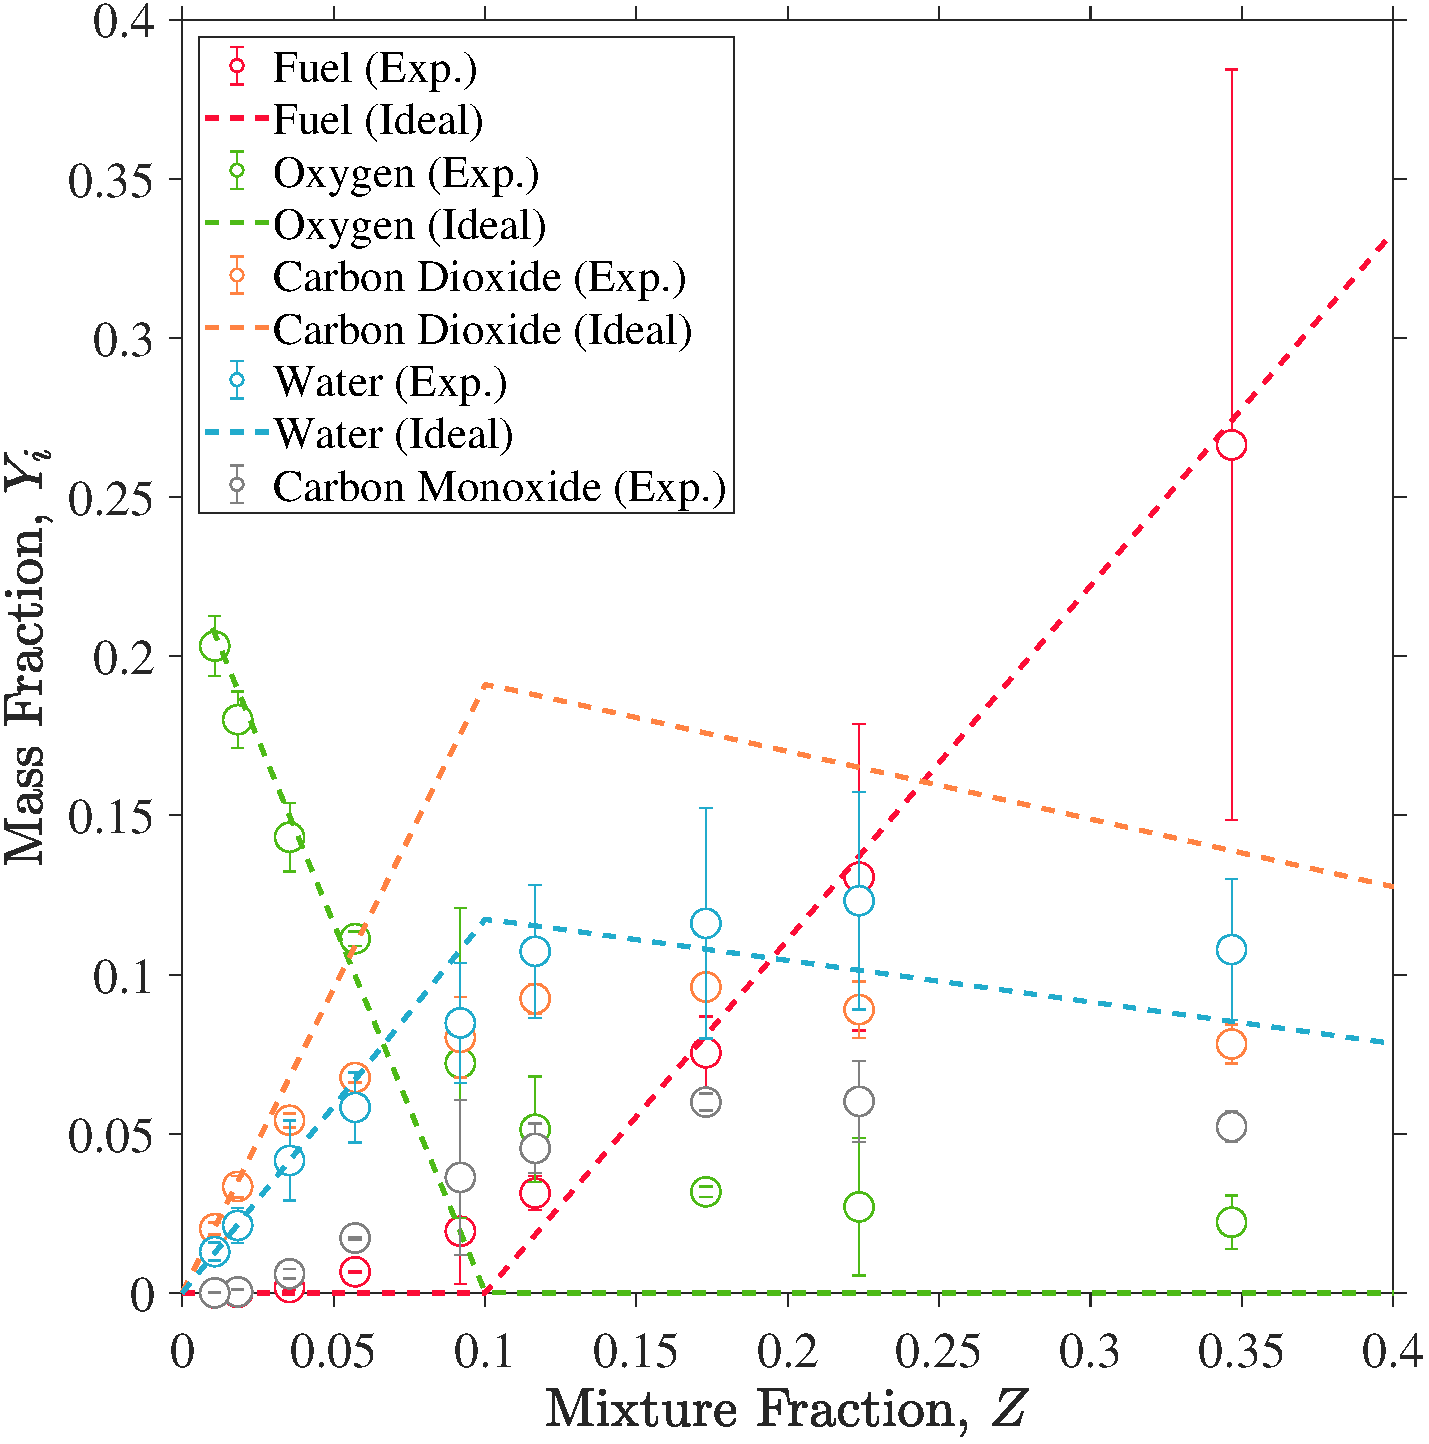
\includegraphics[width=\textwidth,keepaspectratio]{Adjusted_FuelEthanol_Mixture_Fraction_Intermediate_Plot.pdf}
	\caption[Mean mass fractions as a function of mixture fraction, ethanol]{Mean mass fractions as a function of mixture fraction, ethanol. The uncertainty of the mean mass fractions shown here is defined in Section~\ref{ssec:Uncertainty of Mass Fractions}.}
	\label{fig:Ethanol_Mix_Frac}
\end{figure}

\begin{figure}[!]
	\centering
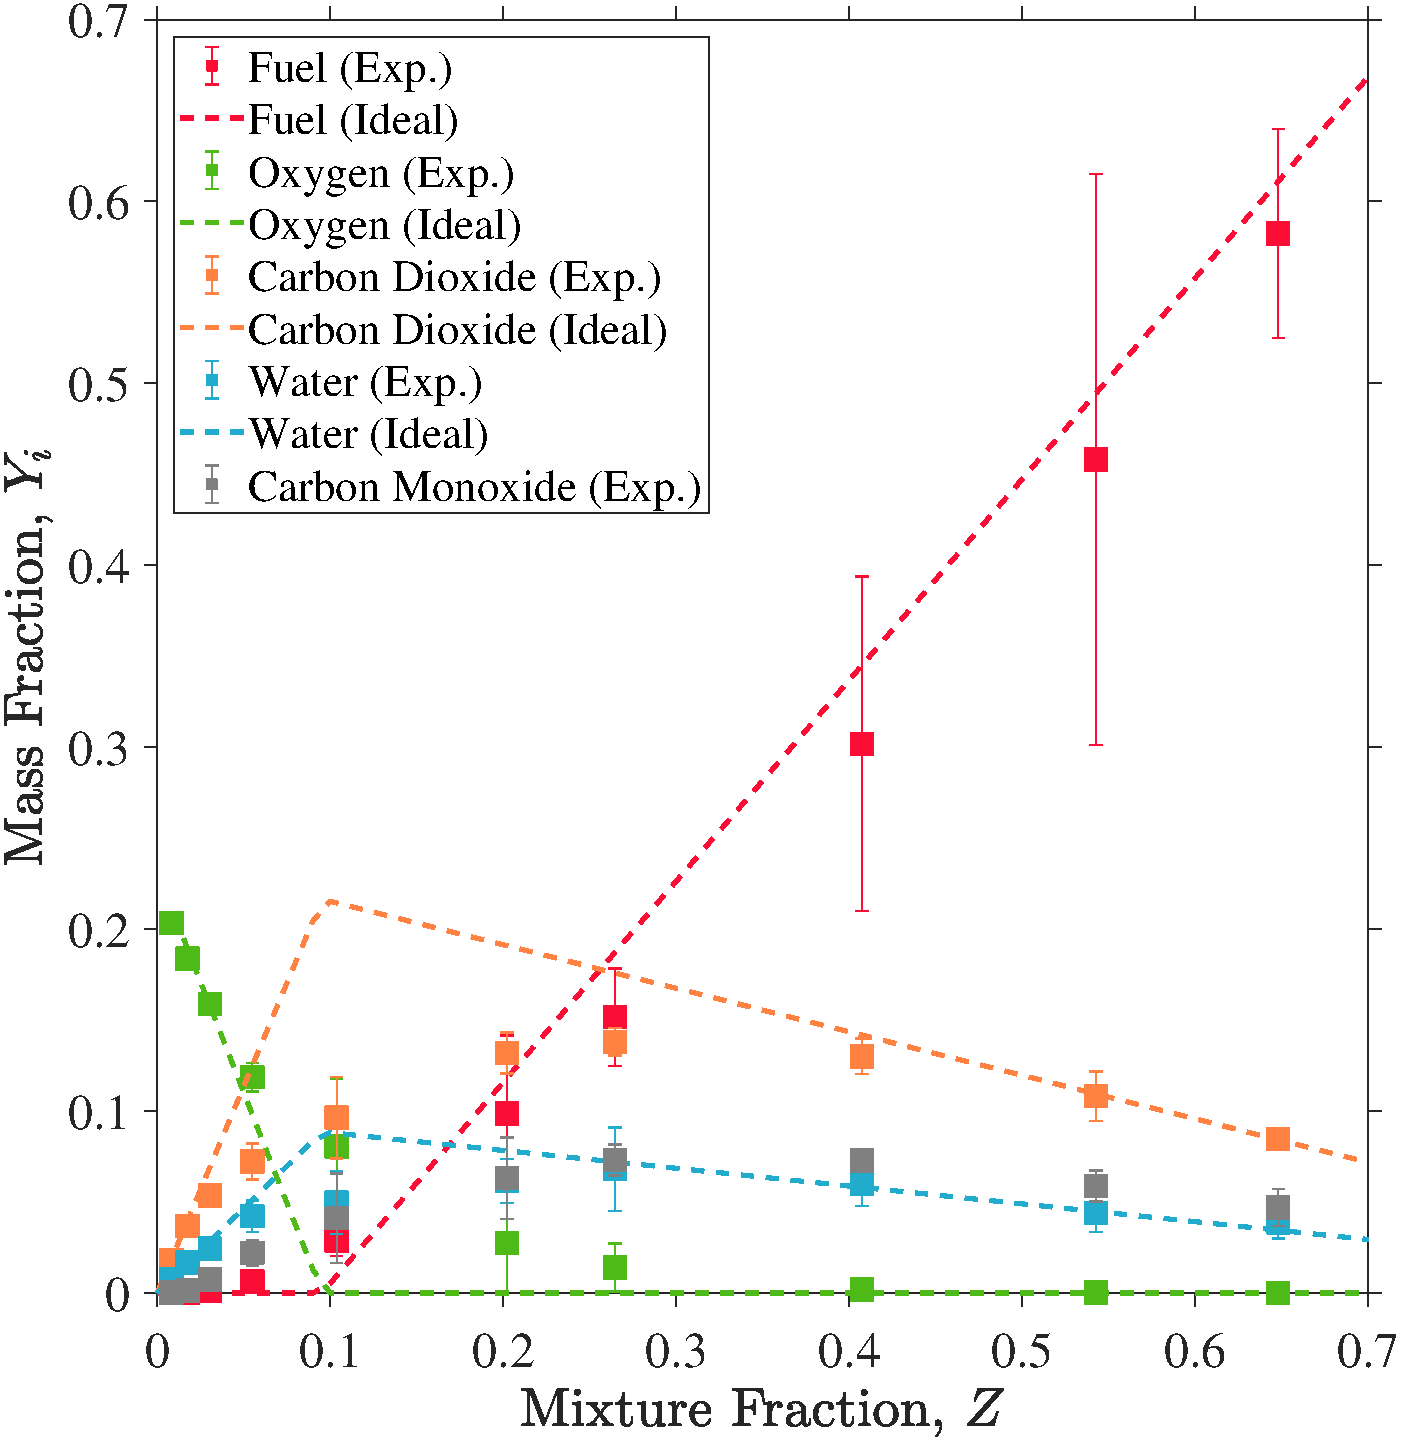
\includegraphics[width=\textwidth,keepaspectratio]{Adjusted_FuelAcetone_Mixture_Fraction_Intermediate_Plot.pdf}
	\caption[Mean mass fractions as a function of mixture fraction, acetone]{Mean mass fractions as a function of mixture fraction, acetone. The uncertainty of the mean mass fractions shown here is defined in Section~\ref{ssec:Uncertainty of Mass Fractions}.}
	\label{fig:Acetone_Mix_Frac}
\end{figure}

\begin{figure}[!]
	\centering
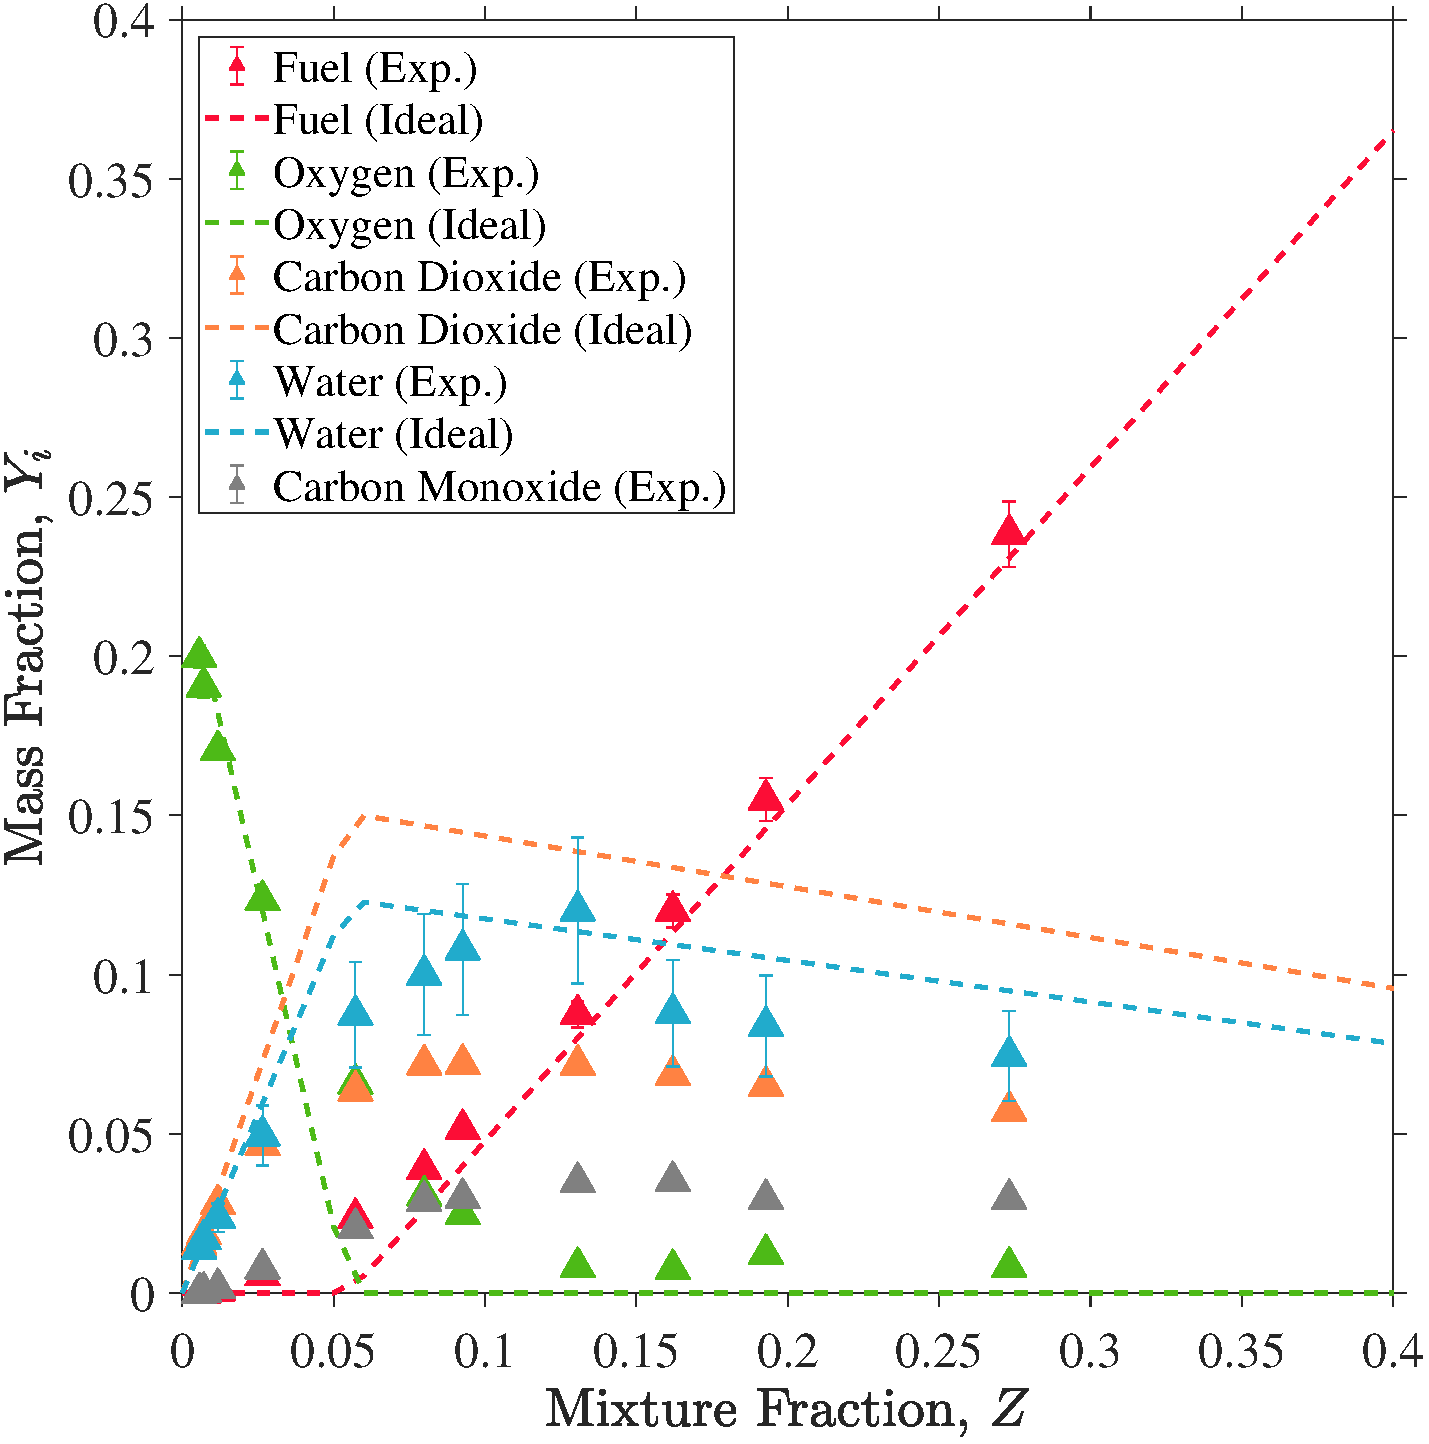
\includegraphics[width=\textwidth,keepaspectratio]{Adjusted_FuelMethane_Mixture_Fraction_Intermediate_Plot.pdf}
	\caption[Mean mass fractions as a function of mixture fraction, methane]{Mean mass fractions as a function of mixture fraction, methane. The uncertainty of the mean mass fractions shown here is defined in Section~\ref{ssec:Uncertainty of Mass Fractions}.}
	\label{fig:Methane_Mix_Frac}
\end{figure}

\begin{figure}[!]
	\centering
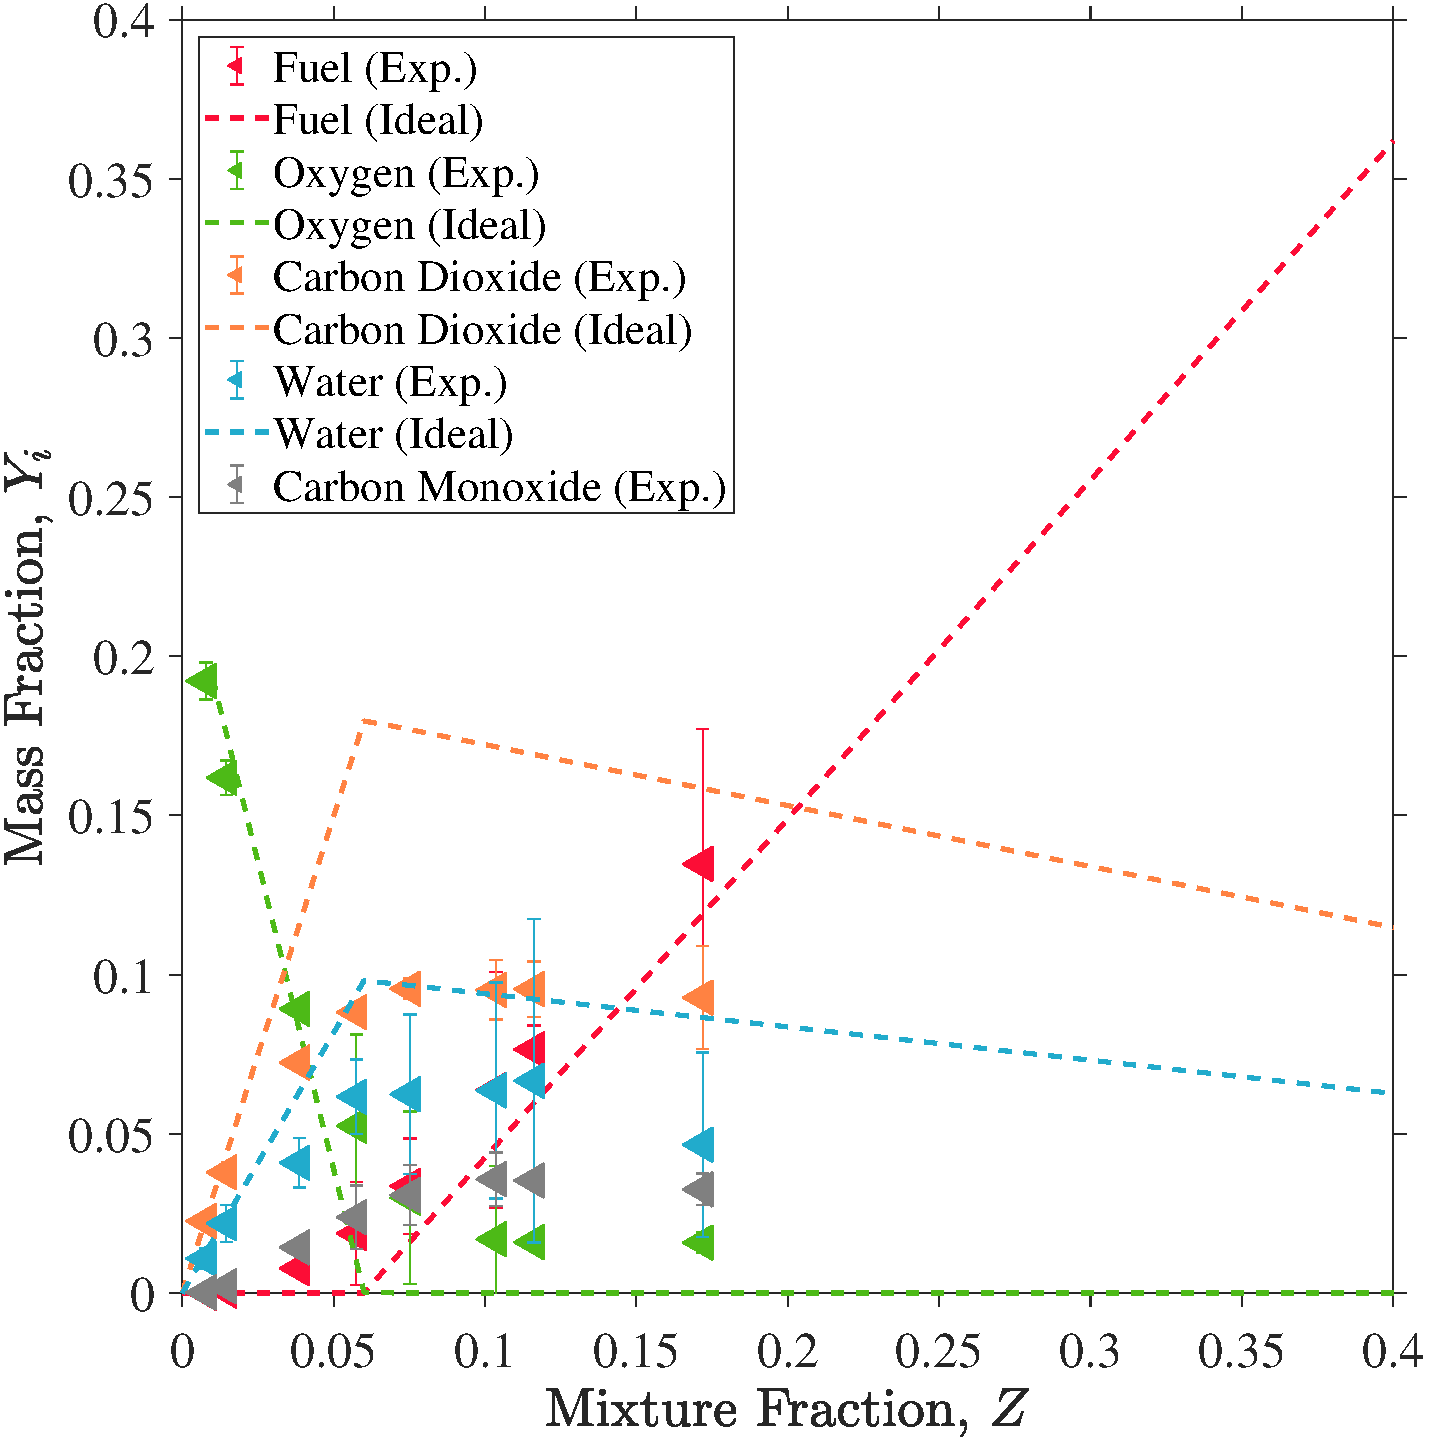
\includegraphics[width=\textwidth,keepaspectratio]{Adjusted_FuelPropane 20KW_Mixture_Fraction_Intermediate_Plot.pdf}
	\caption[Mean mass fractions as a function of mixture fraction, propane (20~kW)]{Mean mass fractions as a function of mixture fraction, propane (20~kW). The uncertainty of the mean mass fractions shown here is defined in Section~\ref{ssec:Uncertainty of Mass Fractions}.}
	\label{fig:Propane20kW_Mix_Frac}
\end{figure}

\begin{figure}[!]
	\centering
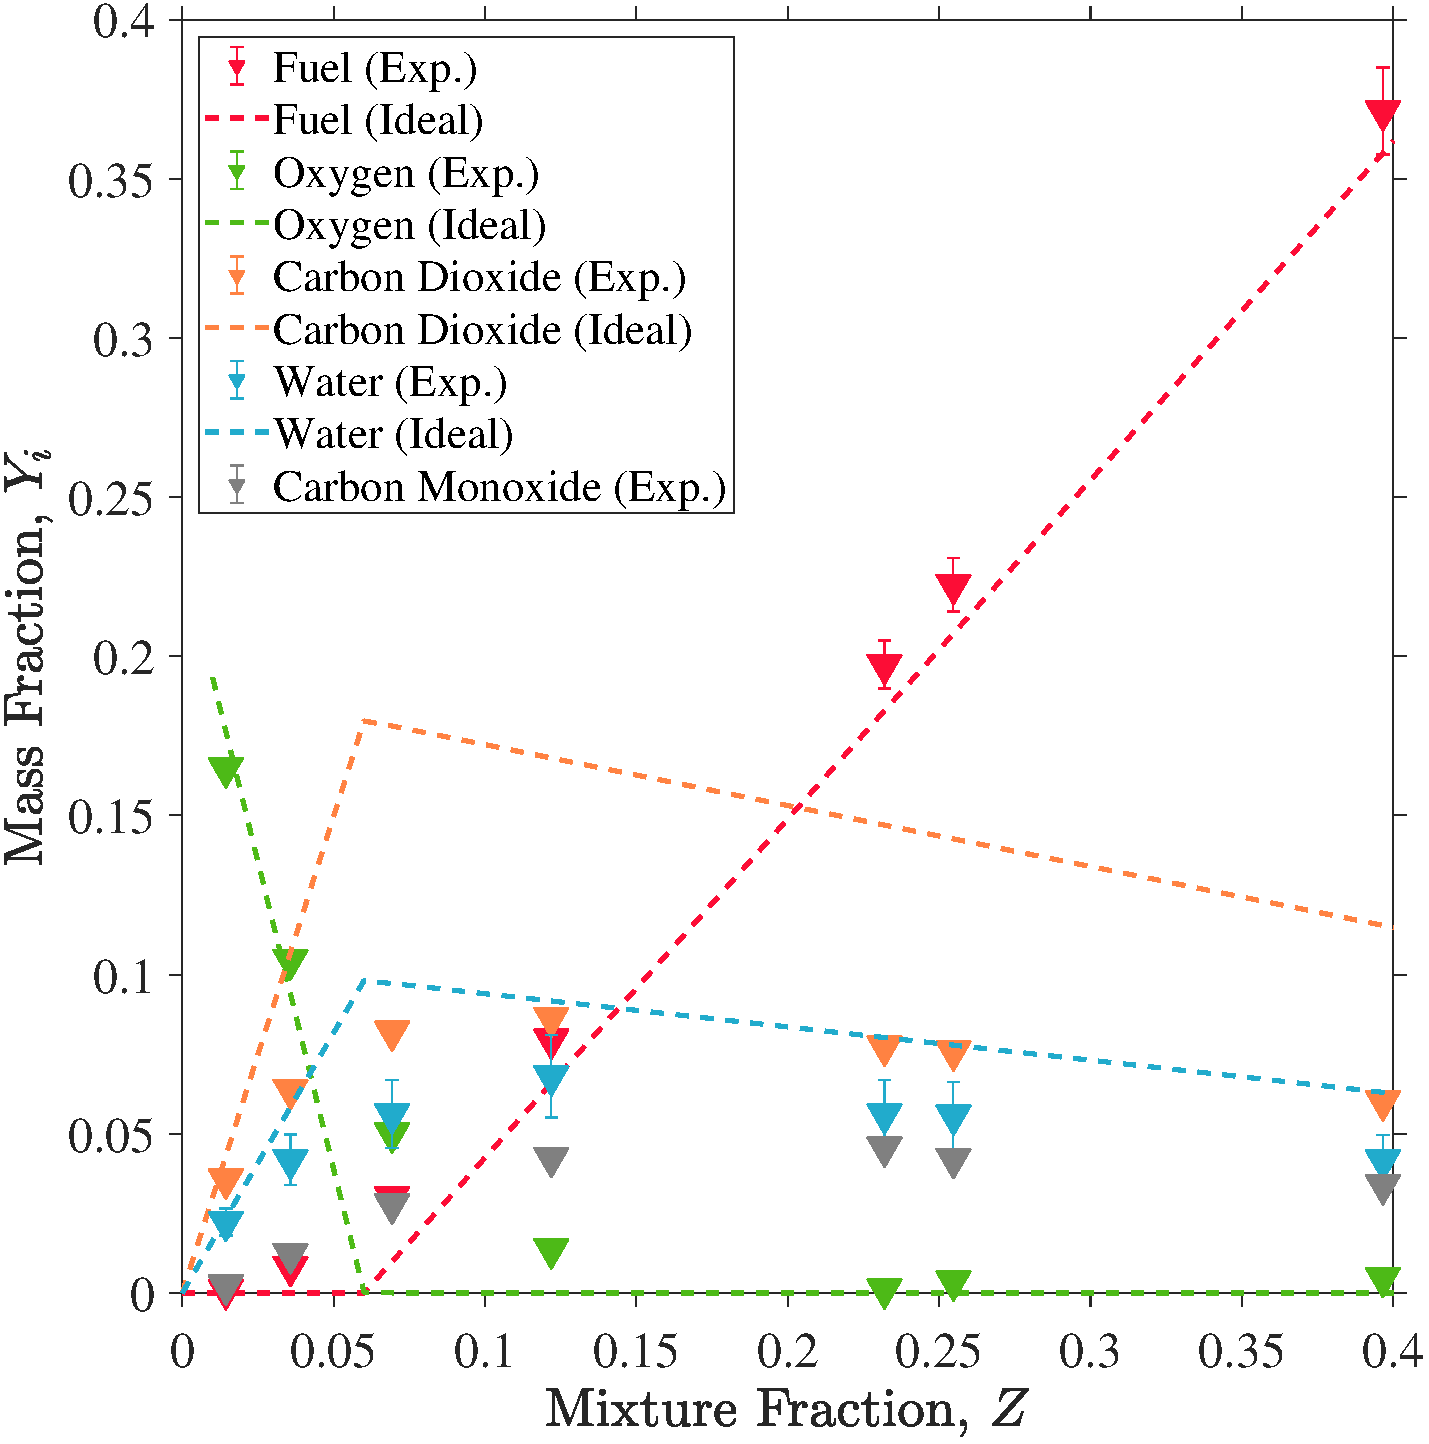
\includegraphics[width=\textwidth,keepaspectratio]{Adjusted_FuelPropane 34KW_Mixture_Fraction_Intermediate_Plot.pdf}
	\caption[Mean mass fractions as a function of mixture fraction, propane (34~kW)]{Mean mass fractions as a function of mixture fraction, propane (34~kW). The uncertainty of the mean mass fractions shown here is defined in Section~\ref{ssec:Uncertainty of Mass Fractions}.}
	\label{fig:Propane34kW_Mix_Frac}
\end{figure}

Where the mixture fraction is much less than stoichiometric, all major gas species are in close agreement with the ideal state relations; the measured mass fractions of unburned fuel and $\ch{CO}$ are nearly zero, and the $\ch{O_2}$ is close to its respective theoretical value. The measured mass fraction of $\ch{CO_{2}}$ and $\ch{H_{2}O}$ are found to peak close to the stoichiometric mixture fraction. In the fuel-rich region, the measured mass fraction of $\ch{CO_{2}}$ differs considerably from the ideal state relation due to the substantial portion of $\ch{CO}$ and soot.


\clearpage

\section{Conclusion}
\label{sec:Conclusion}
In summary, time-averaged local measurements of temperature and gas species concentrations are made to characterize the structure of methanol, ethanol, and acetone 30~cm diameter pool fires and \textcolor{red}{37~cm effective diameter methane and propane pool fires} steadily burning in a quiescent environment. A verification scheme is developed to verify the gas species measurements that considered  the accuracy of the calibration and the overall stoichiometry of combustion for each fuel. The gas species measurements are favorably compared to the idealized SCR values, which lends confidence to the veracity of the measurements. These local measurements complement previous measurements and provide insight into the complex chemical structure of medium-scale pool fires.

\section*{Acknowledgments}
The authors would like to acknowledge Kevin McGrattan, who aided in the editing of this report.

\clearpage

\section*{References}
\addcontentsline{toc}{section}{References}
\bibliographystyle{unsrt}
\bibliography{References}


\clearpage


\appendix
\numberwithin{equation}{section}
\makeatletter
% "activate" the preparatory code, but for section-level headers only
\newcommand{\section@cntformat}{Appendix:\ }
\makeatother

\section{Uncertainty Analysis of Pool Fire Parameters}\label{sec:Uncertainty_Pool_Fire_Parameters}

\subsection{Mass Burning Rate}
\label{ssec:Mass_Burning_Flux}

\textcolor{red}{For liquid fuels,} the mean mass burning rate, $\dot{m}$, is determined by weighing the fuel reservoir at the start and end of the steady burning stage using a Precisa XB-6200C Precision balance, calibrated using a collection of standard weights. The Type A evaluation of uncertainty is the standard deviation in the measurements made during replicate experiments, $s_{\scriptscriptstyle \dot{m_l}}$. The Type B evaluation of uncertainty is the reported accuracy of the balance, 0.01~g, divided by the time interval. The Type A uncertainty dominates; thus, the standard uncertainty of liquid fuels is approximately the standard deviation of the multiple measurements:

\begin{equation}
\label{eq:mass_rate_uncertainty_liquid}
u_{\scriptscriptstyle \dot{m}} \approx s_{\scriptscriptstyle \dot{m_l} }
\end{equation}

\textcolor{red}{For gas fuels, $\dot{m}$ is determined by the flow of gas controlled via a Brooks mass flow controller, Model 5863, configured to nitrogen. The Type A evaluation of uncertainty is the standard deviation in the measurements made during replicate experiments, $s_{\scriptscriptstyle \dot{m_g}}$. The Type B evaluation of uncertainty of the controller is reported to be 1\% of its full scale, 500~SLPM. The Type B uncertainty dominates; thus, the standard uncertainty of gas fuel is approximately the bias uncertainty of the mass flow controller, $u_{\scriptscriptstyle {\rm{MFC}}}$}.

\begin{equation}
\label{eq:mass_rate_uncertainty_gas}
u_{\scriptscriptstyle \dot{m}} \approx u_{\scriptscriptstyle {\rm{MFC}}}
\end{equation}



\subsection{Heat Release Rate and $Q^*$ }
\label{ssec:Heat_Release_Rate}

The heat release rate, $\dot{Q}$, is the product of the fuel mass loss rate, $\dot{m}$, and the heat of combustion, $\Delta H$. The relative uncertainty of the former is far greater than the latter, thus:
\begin{equation}
\label{eq:heat_release_rate_uncertainty}
u_{\scriptscriptstyle \dot{Q}} \approx \Delta H \, u_{\dot{m}}
\end{equation}
The uncertainty of ${Q^*}$, is dominated by the relative uncertainty of $\dot{Q}$, thus:
\begin{equation}
\label{eq:Q*_uncertainty}
u_{\scriptscriptstyle {Q^*}} \approx \frac{u_{\scriptscriptstyle \dot{Q}}}{c_{p}\rho_\infty T_\infty \sqrt{g} \, D^{5/2}}
\end{equation}

\subsection{Mean Flame Height}
\label{ssec:Mean_Flame_Height}

The mean flame height, ${L_{\rm{f}}}$, is determined using photographic analysis as described in Section~\ref{sec:Experiments}. The Type A evaluation of uncertainty is the standard deviation of the height measurements, $s_{\scriptscriptstyle L_{\rm{f}}}$, made for each frame. The uncertainty of the distance measurement for each frame is relatively small, 0.1~\%, and thus the standard uncertainty is approximately the standard deviation of the heights over multiple frames:

\begin{equation}
\label{eq:mean_flame_height}
u_{\scriptscriptstyle L_{\rm{f}}} \approx s_{\scriptscriptstyle{L_{\rm f}}}
\end{equation}


\subsection{Uncertainty Analysis of Temperature Measurements}
\label{sec:Uncertainty_Temperature_Measurements}
The uncertainty of the temperature measurements is estimated from Type A and Type B uncertainty. The Type A evaluation of uncertainty is the standard deviation of the corrected temperature measurements made at each flame location. The bias error sources, Type B uncertainty, in the S-type thermocouple, $u_{\rm inst}$, used to measure temperature (\SI{1.5}{\degree C}) of the gas sample injected is relatively small compared to the Type A uncertainty.

\textcolor{red}{\subsection{Uncertainty Analysis of Velocity Measurements}}
\textcolor{red}{The mean and standard deviation for the velocity was obtained from the multiple pressure transducers at a specific measurement position. The uncertainty associated with using the measurements from multiple pressure transducers contributed to the combined uncertainty of the gas velocity. Ref.~\cite{Sung2021} provides a detailed description of the velocity uncertainty methodology.}

\textcolor{red}{The time-averaged gas velocity (SYMBOL) and RMS are measured and the uncertainty is estimated from Eq.~\ref{eq:Vel_g}. The gas density in the equation is determined using the thermocouple temperature data.  The mean and standard deviation of the gas velocity obtained from each pressure transducer is estimated from repeat measurements.  The parameters and their data type used in the uncertainty analysis are described in detail in Ref.~\cite{Sung2021}. Temperature-dependent gas properties are taken as those of air and the temperature-dependent emissivity and thermophysical properties of platinum are taken from the literature~\cite{Sung2021}.}

\textcolor{red}{The relative uncertainty of the thermocouple temperature is carefully considered in the velocity uncertainty analysis as it affects the temperature-dependent thermophysical properties of the air in  Eq.~\ref{eq:Vel_g}, influencing the propagation of error~\cite{Sung2021}. The relative uncertainties of the bead diameter and the time derivative of the measured thermocouple bead temperature are estimated to be 5\% based on Ref.~\cite{Sung2021}.}

\pagebreak

\section{Figures of Time-Averaged Bead Temperature Readings}\label{sec:Bead_Temp}

\subsection{Methanol}
\label{ssec:Methanol_Bead_Temp}

\begin{figure}[!h]
	\centering
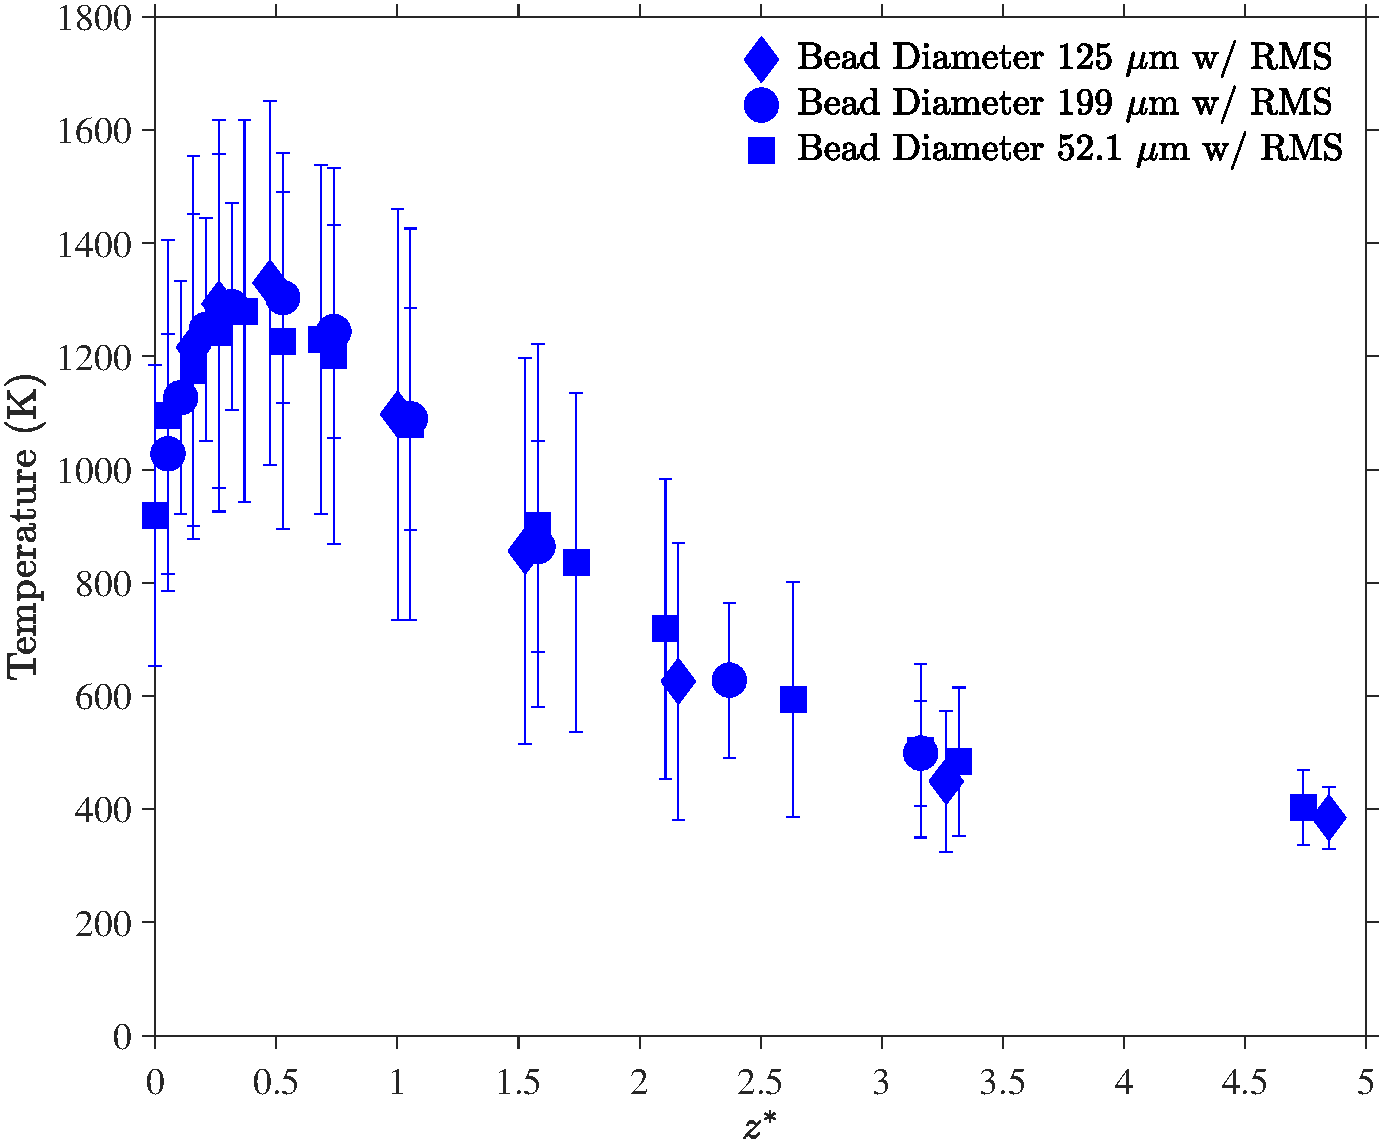
\includegraphics[width=10.25cm,keepaspectratio]{Methanol_Bead_Temperature.pdf}
	\caption[Mean and RMS centerline bead temperature profile of nethanol]{Mean and root mean square (RMS) centerline bead temperature profiles of methanol as a function of $z^*$}
	\label{fig:Methanol_Bead_Temp}
\end{figure}

\pagebreak

\subsection{Ethanol}
\label{ssec:Ethanol_Bead_Temp}
\begin{figure}[h!]
	\centering
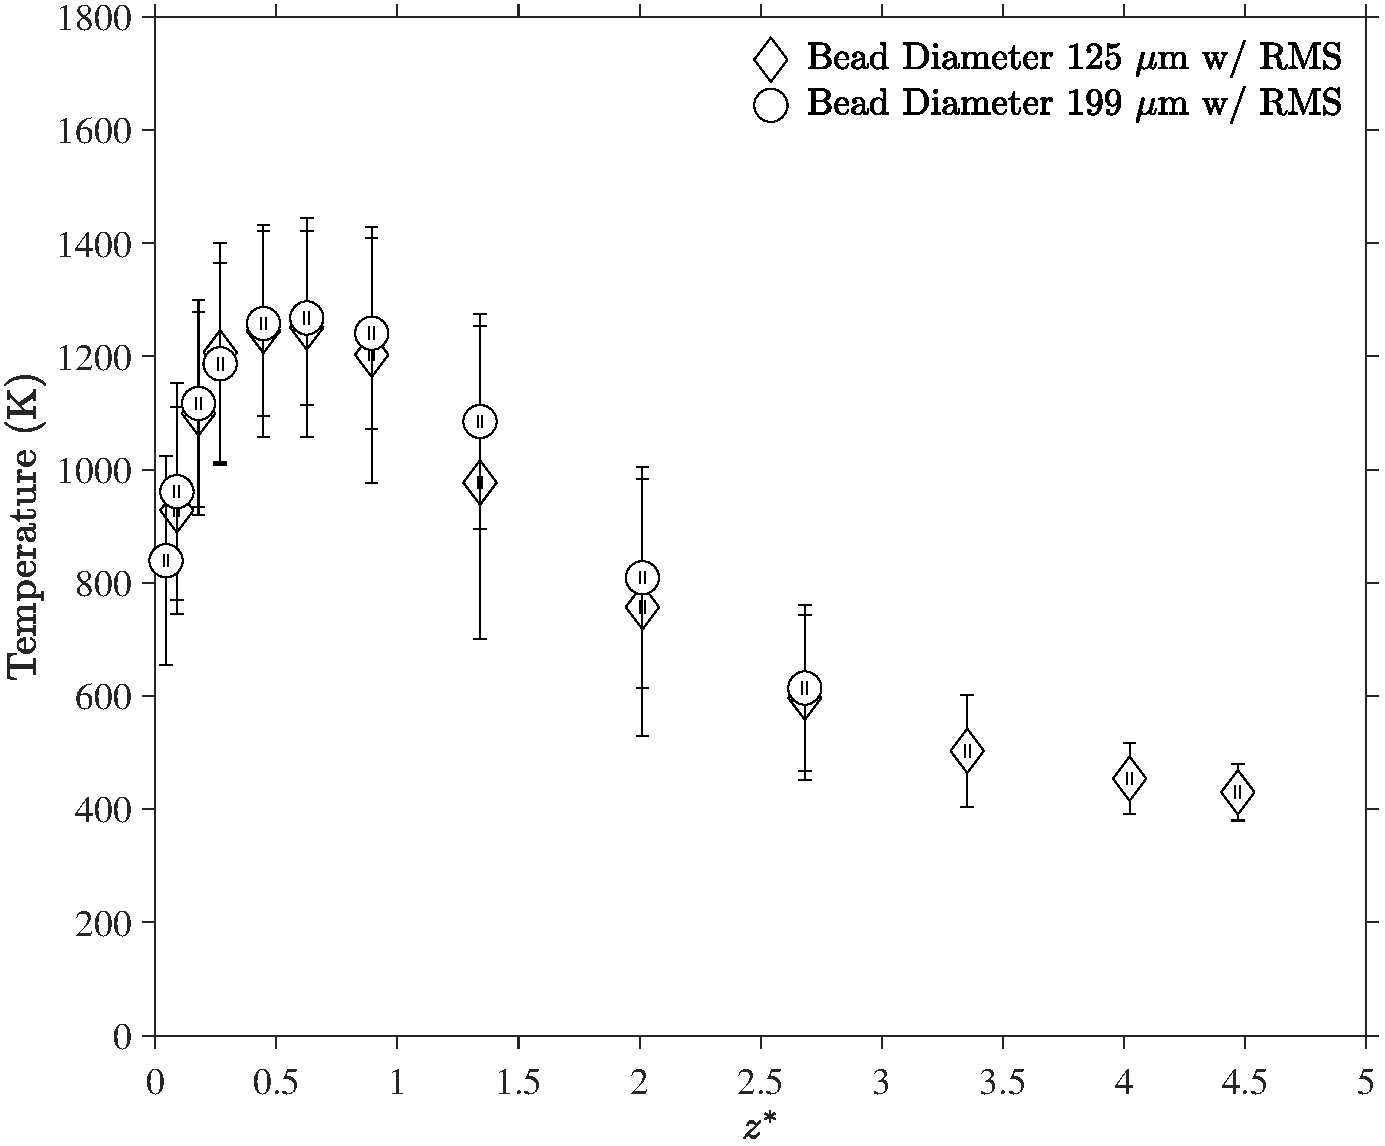
\includegraphics[width=10.5cm,keepaspectratio]{Ethanol_Bead_Temperature.pdf}
	\caption[Mean and RMS centerline bead temperature profile of ethanol]{Mean and root mean square (RMS) centerline bead temperature profiles of ethanol as a function of $z^*$}
	\label{fig:Ethanol_Bead_Temp}
\end{figure}

\pagebreak

\subsection{Acetone}
\label{ssec:Acetone_Bead_Temp}
\begin{figure}[!h]
	\centering
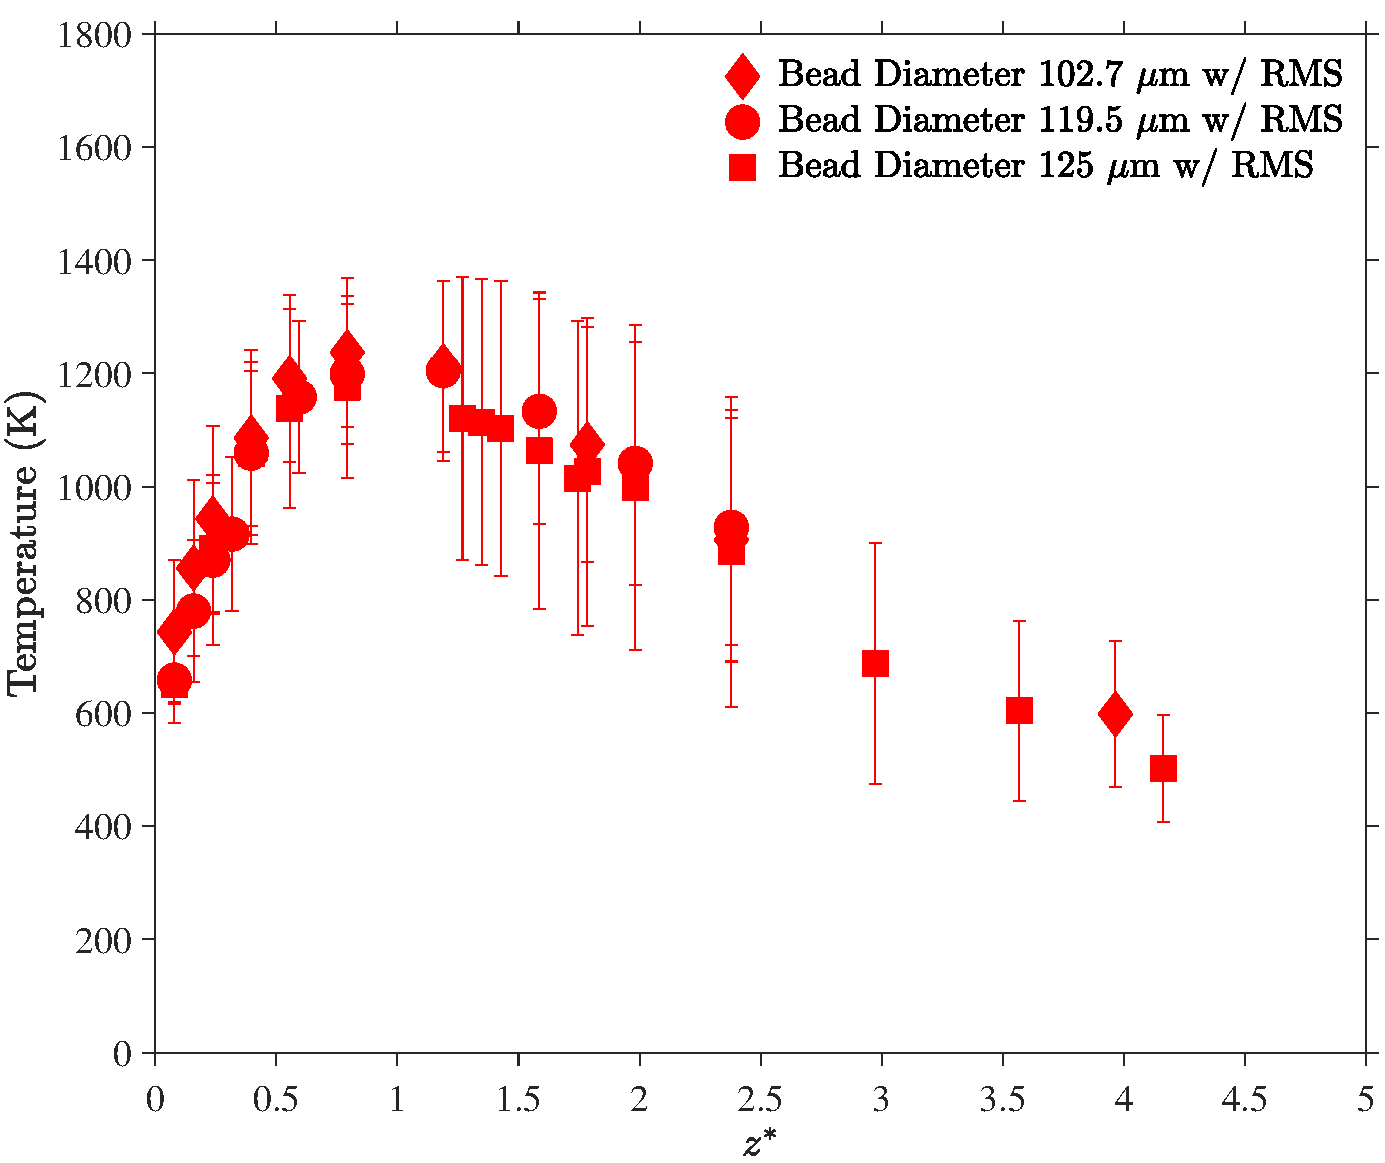
\includegraphics[width=10.5cm,keepaspectratio]{Acetone_Bead_Temperature.pdf}
	\caption[Mean and RMS centerline bead temperature profile of acetonel]{Mean and root mean square (RMS) centerline bead temperature profiles of acetone as a function of $z^*$}
	\label{fig:Acetone_Bead_Temp}
\end{figure}

\pagebreak

\subsection{Methane}
\label{ssec:Methane_Bead_Temp}
\begin{figure}[!h]
	\centering
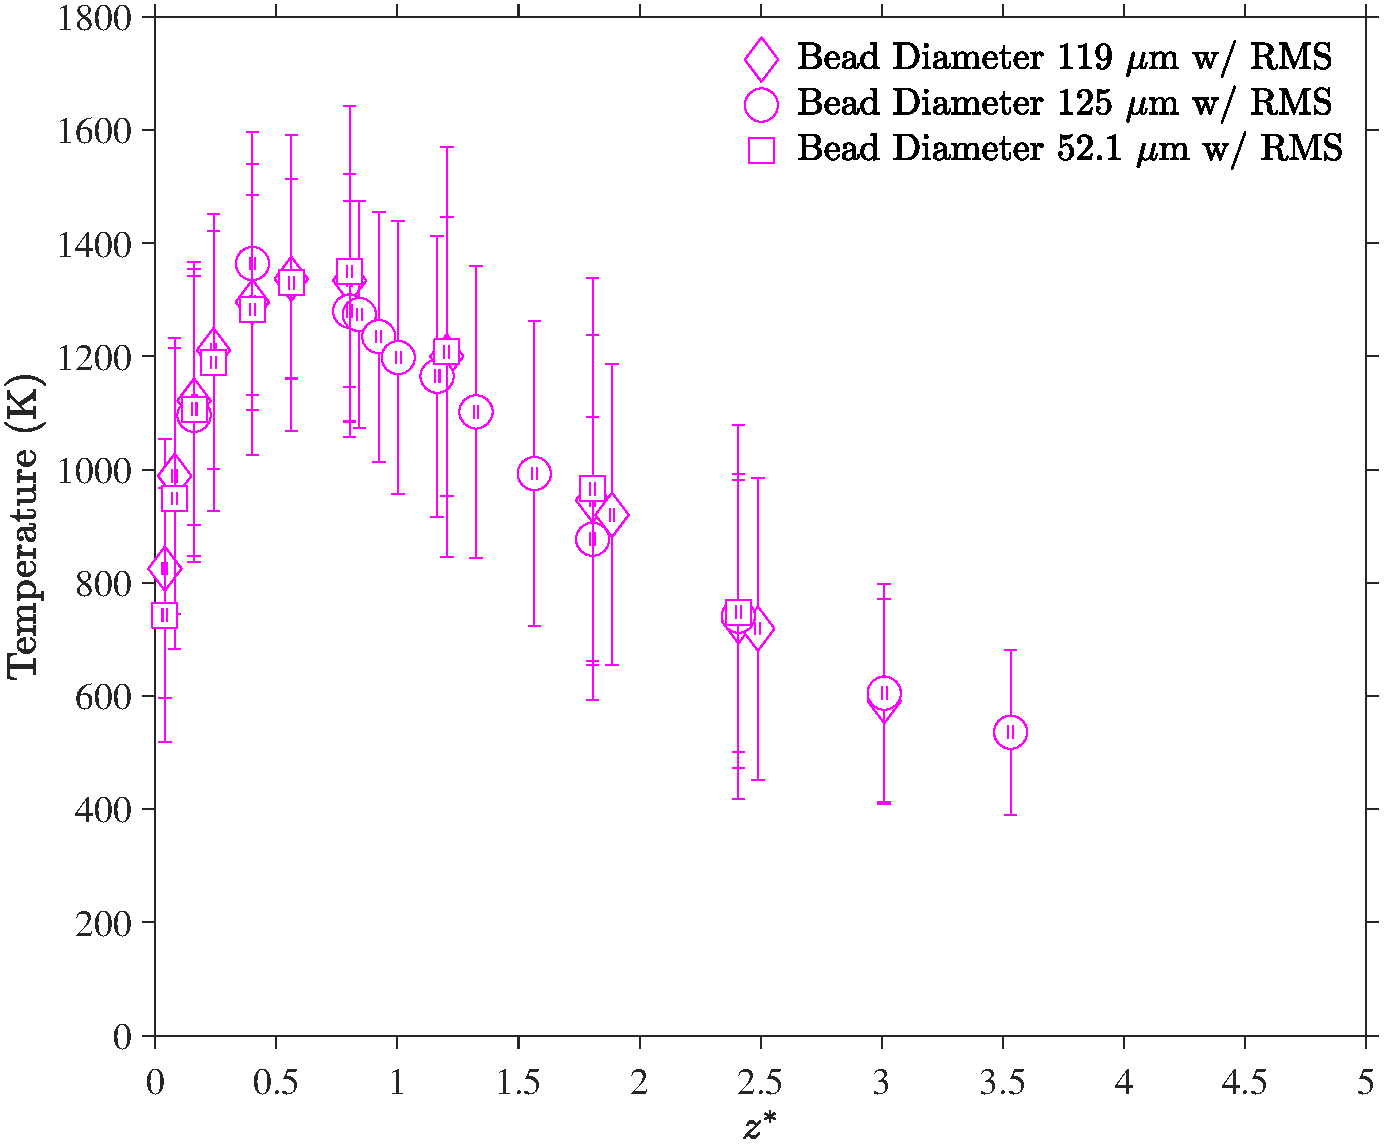
\includegraphics[width=10.5cm,keepaspectratio]{Methane_Bead_Temperature.pdf}
	\caption[Mean and RMS centerline bead temperature profile of methane]{Mean and root mean square (RMS) centerline bead temperature profiles of methane as a function of $z^*$}
	\label{fig:Methane_Bead_Temp}
\end{figure}

\pagebreak

\subsection{Propane (20 kW)}
\label{ssec:Propane20KW_Bead_Temp}
\begin{figure}[!h]
	\centering
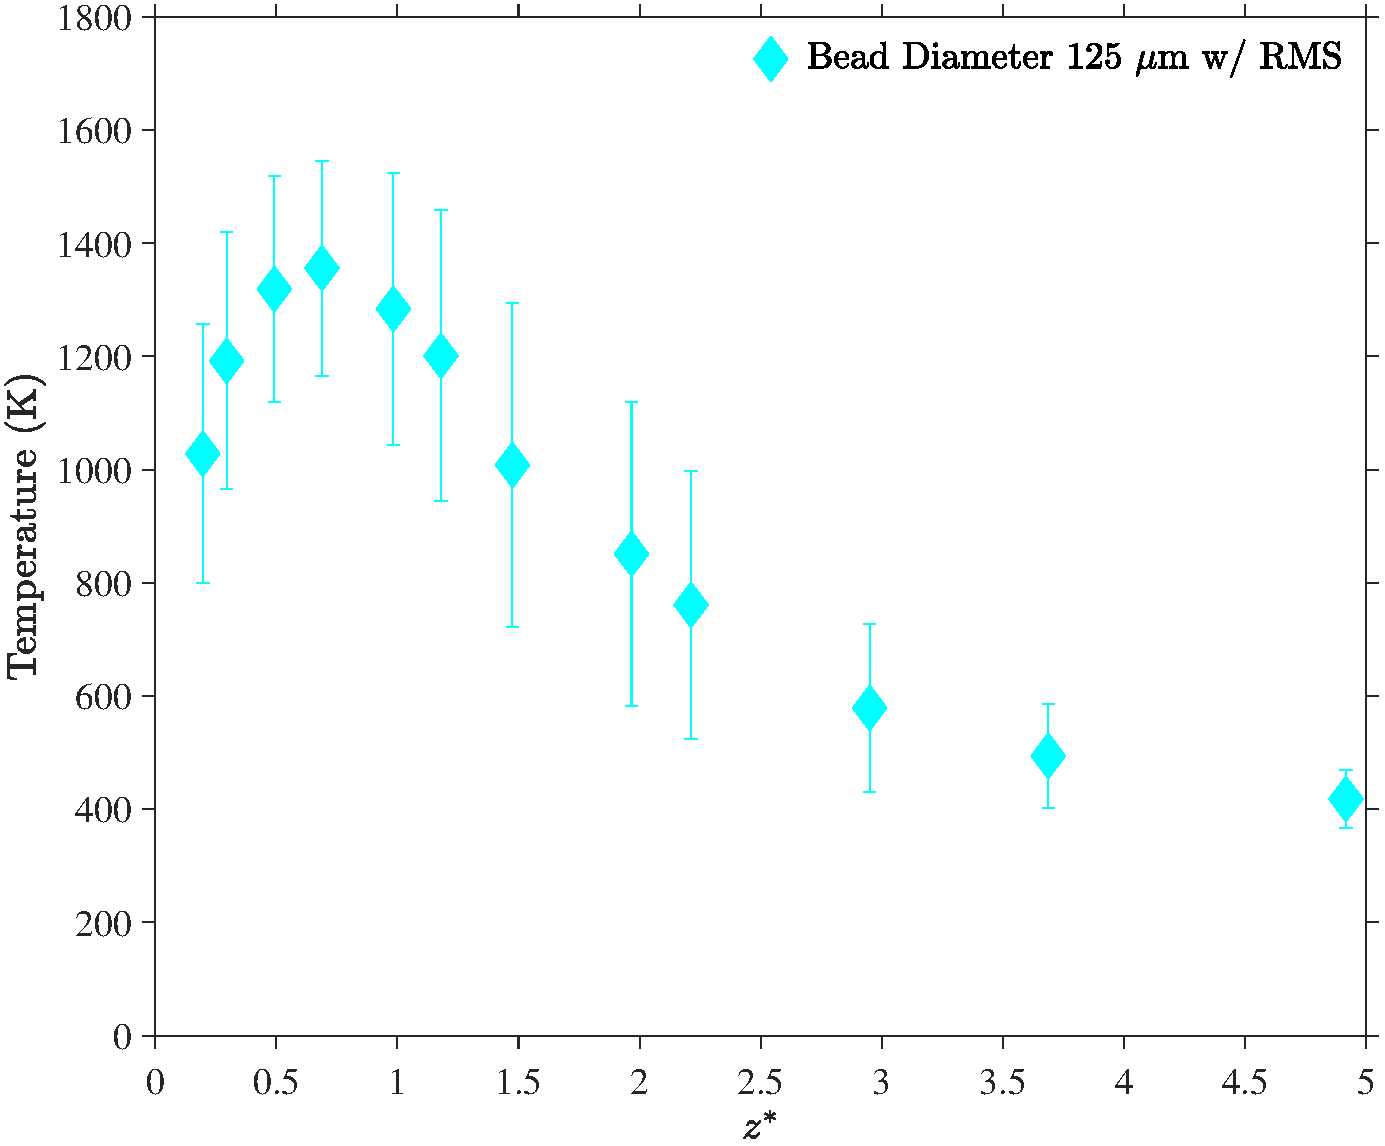
\includegraphics[width=10.5cm,keepaspectratio]{Propane 20KW_Bead_Temperature.pdf}
	\caption[Mean and RMS centerline bead temperature profile of a 20~kW propane fire]{Mean and root mean square (RMS) centerline bead temperature profiles of a 20~kW propane fire as a function of $z^*$}
	\label{fig:Propane20KW_Bead_Temp}
\end{figure}

\pagebreak

\subsection{Propane (34 kW)}
\label{ssec:Propane34KW_Bead_Temp}
\begin{figure}[!h]
	\centering
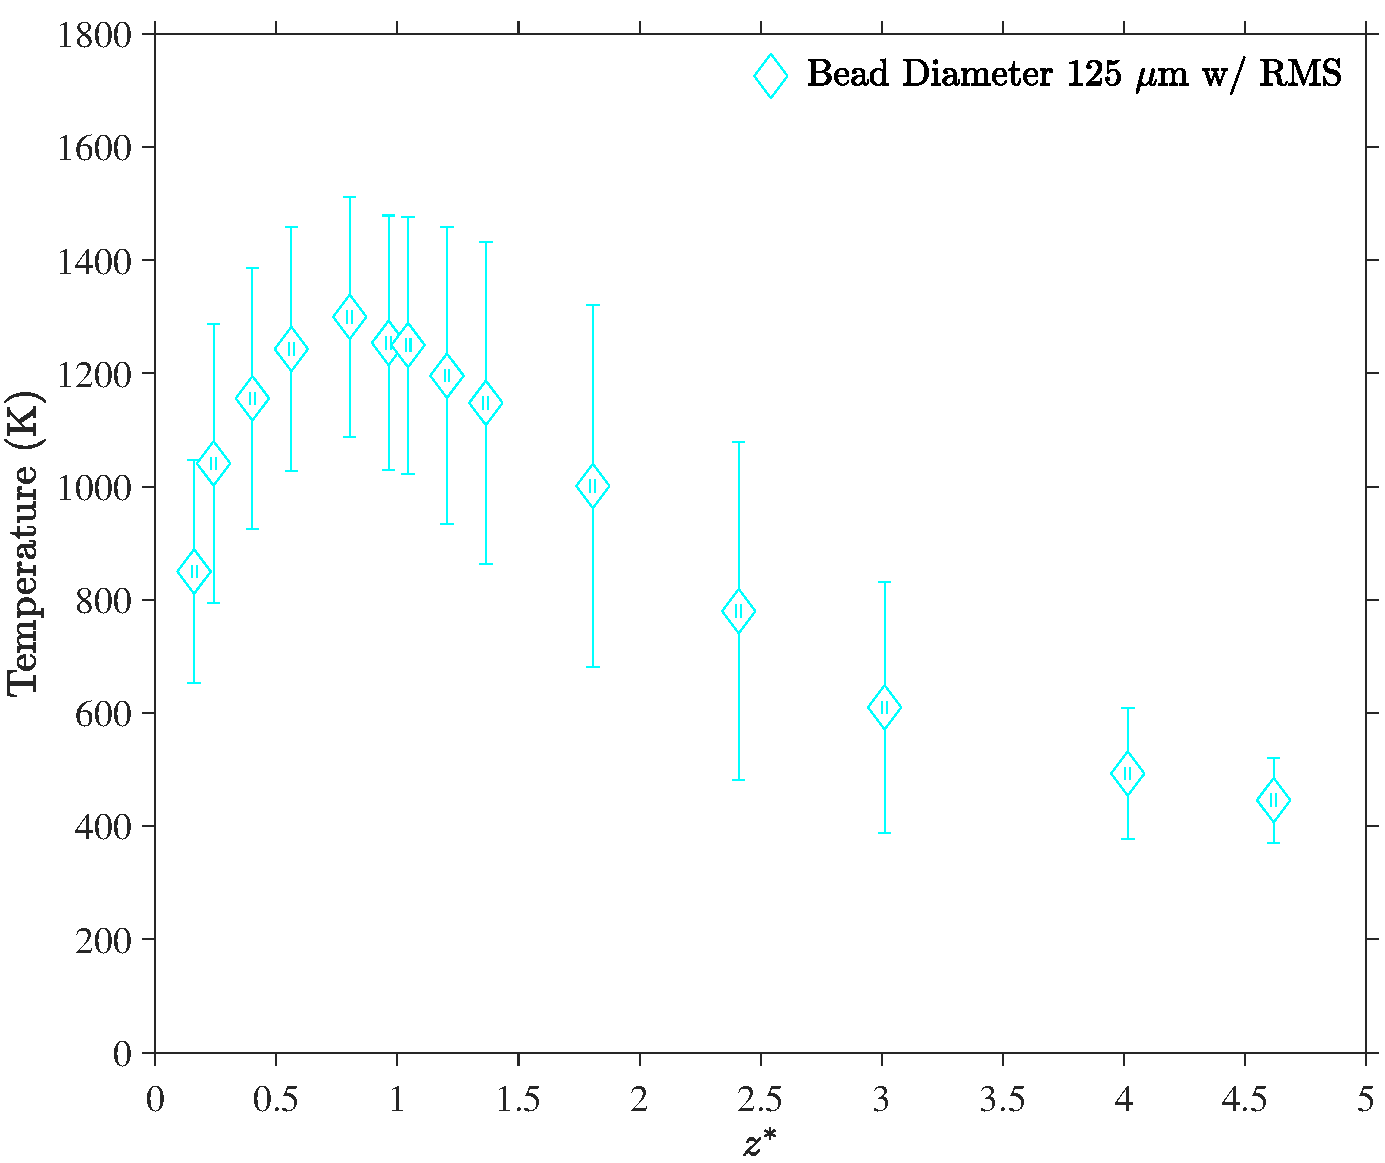
\includegraphics[width=10.5cm,keepaspectratio]{Propane 34KW_Bead_Temperature.pdf}
	\caption[Mean and RMS centerline bead temperature profile of a 34~kW propane fire]{Mean and root mean square (RMS) centerline bead temperature profiles of a 34~kW propane fire as a function of $z^*$}
	\label{fig:Propane34KW_Bead_Temp}
\end{figure}

\pagebreak

\section{Estimating the Characteristic Length of the Regime of Influence}\label{sec:Regime_of_Influence}

When extracting a gas sample from a fire scene, a probe is typically placed in an arbitrary location within the fire, where it can sample gases at a preset volumetric flow rate, $\rm{\dot{Q}}$. Ideally, the probe inlet flow should be minimal, such that it does not disrupt the flow field created from the fire. It is assumed that, in most cases, the flow field around the inlet of the sampling probe is assumed to be vertical.

The regime of influence can be defined as the area of which the presence of the sampling probe disrupts the velocity profile. Figure~\ref{fig:Potential Flow} shows a 2D vector flow field with a sink placed at the center and the regime of influence bounded by the dotted line. The characteristic length of the regime of influence, $L$, is defined as the distance from the sink which the velocity profile is approximately ($>$ 99\%) of dominant.
\begin{figure}[h!]
	\centering
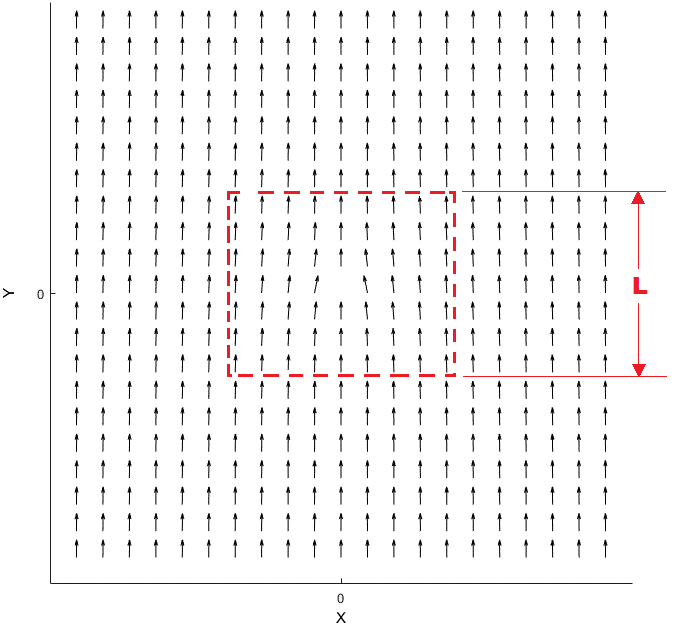
\includegraphics[width=8.45cm,keepaspectratio]{Potential_Flow.png}
	\caption{A 2D vector flow field with a sink placed at the origin. The dotted lines defines the regime of influence with a characteristic length $L$}
	\label{fig:Potential Flow}
\end{figure}

The velocity profile, derived from potential flow is defined below:
\begin{equation}
\label{eq:u-velocity}
u(x,y,z)=\frac{-\rm{\dot{Q}}}{8\pi}~\frac{x}{({x^2+y^2+z^2})^{\frac{3}{2}}}
\end{equation}
\begin{equation}
\label{eq:v-velocity}
v(x,y,z)=\frac{-\rm{\dot{Q}}}{8\pi}~\frac{y}{({x^2+y^2+z^2})^{\frac{3}{2}}}+V_{\infty}
\end{equation}
where $V_{\infty}$ is the velocity profile, assumed to be completely vertical surrounding the sampling probe. 
\begin{equation}
\label{eq:w-velocity}
w(x,y,z)=\frac{-\rm{\dot{Q}}}{8\pi}~\frac{z}{({x^2+y^2+z^2})^{\frac{3}{2}}}
\end{equation}
At (0,$L$,0) the vertical velocity can be defined as
\begin{equation}
\label{eq:v-velocity_atL}
0.99~V_{\infty}-V_{\infty}=\frac{-\rm{\dot{Q}}}{8\pi}~\frac{L}{L^3}+V_{\infty}
\end{equation}
Equation~\ref{eq:v-velocity_atL} can then be rearranged to solve for $L$.
\begin{equation}
\label{eq:char_length}
L=\sqrt{\frac{\rm{\dot{Q}}}{8\pi~0.01~V_{\infty}}}
\end{equation}

\pagebreak

\section{Elution times of combustion species using a Select for Permanent Gasses-Dual Column}\label{sec:Elution Times}

A table of the gas species elution times using the method described in Section~\ref{ssec:Gas_Species_Setup}. This method utilizes an Agilent J\&W Select Permanent Gases/\ch{CO2} High-Resolution column is provided below.The column is a parallel configuration consisting of a 25~m x 0.32~mm PoraBOND Q capillary column coupled with a 50~m x 0.53~mm Molsieve $\SI{5}{\angstrom}$ capillary column. 

\begin{table}[h!]

\caption*{ Elution times of gas species from a dual column composed of Molsieve 5A column and PoraBOND Q columns in parallel.}
\label{tab:Elution_Table}
\centering
	%\footnotesize
	\begin{tabular}{clcc}
\specialrule{.2em}{.1em}{.1em} 
%\\[0.0005cm]
\textbf{Retention} &\textbf{Species}&\textbf{Eluted}\\
\textbf{Time (min)} &&\textbf{from}\\
\specialrule{.2em}{.1em}{.1em} 
$6.4$		&	Composite 1		&	PoraBOND Q					\\%&0.2		\\
$6.8$		&	Methane		& 	PoraBOND Q					\\%&0.2		\\
$7.6$		&	Carbon Dioxide	&	PoraBOND Q					\\%&0.2		\\
$9.2$		&	Composite 2		&	PoraBOND Q					\\%&0.2		\\
$9.3$		&	Hydrogen		&	Molsieve $\SI{5}{\angstrom}$		\\%&0.1		\\
$12.7$	&	Water			&	PoraBOND Q					\\%&0.2		\\
$13.8$	&	Argon			&	Molsieve $\SI{5}{\angstrom}$		\\%&0.3		\\
$14.6$	&	Oxygen		&	Molsieve $\SI{5}{\angstrom}$		\\%&0.1		\\
$15.7$	&	Propane		&	PoraBOND Q					\\%&0.1		\\
$19.7$	&	Methanol		&	PoraBOND Q					\\%&0.1		\\
$20.6$	&	Nitrogen		&	Molsieve $\SI{5}{\angstrom}$		\\%&0.3		\\
$24.2$	&	Ethanol		&	PoraBOND Q					\\%&0.5		\\
$24.4$	&	Methane		&	Molsieve $\SI{5}{\angstrom}$		\\%&0.4		\\
$27.4$	&	Acetone		&	PoraBOND Q					\\%&0.8		\\
$29.3$	&	Carbon Monoxide	&	PoraBOND Q					\\%&0.1		\\
$34.7$	&	Benzene		&	PoraBOND Q					\\%&0.1		\\
$43.6$	&	Ethane		&	Molsieve $\SI{5}{\angstrom}$		\\%&0.2		\\
$50.2$	&	Acetylene		&	Molsieve $\SI{5}{\angstrom}$		\\%&0.2		\\
$57.3$	&	Ethylene		&	Molsieve $\SI{5}{\angstrom}$ 		\\%&0.1		\\
$65.2$	&	Propane		&	Molsieve $\SI{5}{\angstrom}$ 		\\%&0.1		\\
\specialrule{.2em}{0em}{.1em} 
\end{tabular}
\end{table}

\pagebreak

\section{Uncertainty Analysis of Gas Species Concentrations} \label{sec:UncertaintyGasSpecies}

\subsection{Uncertainty of Volume Fractions} \label{sec:UncertaintyMoleFrac}
As shown in Eq.~\ref{eq:volume_fraction}, volume fraction, $\bar{X}_{i}$, is calculated from the ratio between the number of moles of a given species, $n_{i}$, and the total number of moles identified, $n_{\rm tot}$. The uncertainty of the measured volume fraction is estimated using the law of propagation of uncertainty after determining the volume fraction of each species:

\begin{equation}
\label{eq:Volume_Frac_Uncertainty}
u_\mathrm{\bar{X}_{i}} = \sqrt{{\left( \frac{\partial \bar{X}_{i}}{\partial n_{i}}\,u_{\scriptscriptstyle n_{i}} \right)}^2+{\left(\frac{\partial \bar{X}_{i}}{\partial n_{\rm tot}}\,u_{\scriptscriptstyle n_{\rm tot}}\right)}^2}
\end{equation}
A coverage factor of 2 is applied to the combined uncertainty to produce a 95~\% confidence interval.

\subsubsection{Number of Moles of a Given Species}
\label{ssec:Number_of_Moles_of_a_Given_Species}

The number of moles of a given species is determined from a calibration function of the integrated peak area of the respective species obtained from the TCD's and the MS's Total Ion Current (TIC) chromatograms. The Type A evaluation of standard uncertainty of the number of moles of a given species is taken as the standard deviation of the measurements obtained from the repeated tests. The Type B evaluation of standard uncertainty is determined from the error in the calibration functions for each species measured by the TCD and MS is further detailed in Appendix~\ref{sec:Uncertainty Analysis of Gas Species Calibrations}. The combined uncertainty is found via quadrature:
\begin{equation}
\label{eq:gasspeciesuncertaintycertainty}
u_{\scriptscriptstyle n_{i}} = \sqrt{ u_{\scriptscriptstyle n_{i,\rm cal}}^2 + s_{\scriptscriptstyle n_{i}}^2}
\end{equation}

\subsubsection{Total Number of Moles Identified}
\label{ssec:Total Number of Moles Identified}
The total number of moles detected is determined from the summation of the number of moles for each species identified by the TCD and TIC chromatograms. Therefore, the uncertainty in the total number of moles identified is the combined uncertainty of all the identified species via quadrature:
\begin{equation}
\label{eq:totalnumberofmolesdetected}
u_{\scriptscriptstyle n_{\rm tot}}=\sqrt{{\sum_{n=1}^{N} s_{\scriptscriptstyle n_{i}}^2}}
\end{equation}
where $N$ is the number of a species identified species in the TCD and TIC chromatogram.

\subsection{Uncertainty of Mass Fractions}
\label{ssec:Uncertainty of Mass Fractions}

Mass fraction of a given species is calculated using its measured volume fraction, $\bar{X_{i}}$, molecular weight, $W_i$ , and the average molecular weight of all detected gas species, $W_{\rm tot}$, as shown in Eq.~\ref{eq:mass_fraction}. The uncertainty of the mass fraction of a given species is estimated from the law of propagation of uncertainty using Eq.~\ref{eq:mass_fraction}.
\begin{equation}\label{eq:Mass_Frac_Uncertainty}
u_\mathrm{\bar{Y}_{i}} = \sqrt{{\left( \frac{\partial \bar{Y}_{i}}{\partial \bar{X}_{i}}\,u_{\scriptscriptstyle \bar{X}_{i}} \right)}^2+{\left(\frac{\partial \bar{Y}_{i}}{\partial W_{\rm tot}}\,u_{\scriptscriptstyle W_{\rm{tot}}}\right)}^2}
\end{equation}

\subsubsection{Uncertainty of the average molecular weight}
\label{ssec:Uncertainty of the average molecular weight}

The uncertainty of the average molecular weight is determined using the law of propagation of uncertainty, which accounted for each detected species measured from the injected sample.
\begin{equation}\label{eq:Uncertainty_Total_MW}
	u_{\scriptscriptstyle W_{\rm{tot}}}=\sqrt{\left(\sum{{u_{\scriptscriptstyle \bar{X}_{i}}}{{W_{i}}}}\right)^2}
\end{equation}

\pagebreak

\section{Uncertainty Analysis of Gas Species Calibrations}\label{sec:Uncertainty Analysis of Gas Species Calibrations}

Peak areas are converted into number of moles, $n_{i}$, using linear calibration curves.
\begin{equation}
\label{eq:Calibration Curve}
n_{i\rm} = a \, (\rm {Area})+b
\end{equation}
The coefficients in the calibration curves are weighted to account for the error of each gas standard used in the calibration procedure. The uncertainty of a number of moles determined from calibration function is estimated using the law of propagation of uncertainty:
\begin{equation}
\label{eq:Given_Moles_Uncertainty}
 u_{\rm \scriptscriptstyle n_{i}} = \sqrt{{\left( \frac{\partial n_{i}}{\partial a}\,u_{\scriptscriptstyle a} \right)}^2+{\left(\frac{\partial {n_{i}}}{\partial b}\,u_{\scriptscriptstyle b}\right)}^2}
\end{equation}
The uncertainties of the slope and intercept in a weighting linear regression are as follows:
\begin{equation}
\label{eq:Slope_Uncertainty}
u_{\rm \scriptscriptstyle a} =\sqrt{\frac{\sum~\frac{1}{u_{n_{i,\rm cal}}}}{(\sum~\frac{\rm{Area}_{i}^2}{{u_{n_{i,\rm cal}}^2}})(\sum~\frac{1}{{u_{n_{i,\rm cal}}^2}})-(\sum~\frac{\rm{Area}_{i}}{{u_{n_{i,\rm cal}}^2}})^2}}
\end{equation}
\begin{equation}
\label{eq:Intercept_Uncertainty}
u_{\rm \scriptscriptstyle b} =\sqrt{\frac{\sum~\frac{\rm{Area}_{i}^2}{u_{n_{i,\rm cal}}}}{(\sum~\frac{\rm{Area}_{i}^2}{{u_{n_{i,\rm cal}}^2}})(\sum~\frac{1}{{u_{n_{i,\rm cal}}^2}})-(\sum~\frac{\rm{Area}_{i}}{{u_{n_{i,\rm cal}}^2}})^2}}
\end{equation}
where $u_{n_{i,\rm cal}}$ is the uncertainty of a known number of moles injected into the GC/MS for calibration.

During calibration, the number of moles of a given species $n_{i,\rm cal}$ are calculated from the product of the total moles injected into the GC/MS, $n_{\rm inj}$, and the known concentration of the particular species in the calibration standard, $C_{i}$.

\begin{equation}
\label{eq:Cal_Moles}
n_{i,\rm cal} = C_{i} \, n_{\rm inj}
\end{equation}
A collection of gas calibration standards for a variety of species are pre-selected to provide a broad range of concentrations. All calibration standards are mixtures of the target gas species with a nitrogen balance, with the exception of one standard balanced in Air. A list of gas standards used in this work, with their respective concentrations and Type B evaluation of standard uncertainty, is provided in Appendix~\ref{sssec:Table of Gas Standards with Error}.

The uncertainty of the number of moles of a given species injected into the GC/MS for calibration is estimated using the law of propagation of uncertainty:

\begin{equation}
\label{eq:Given_Moles_Cal_Uncertainty}
 u_{\rm \scriptscriptstyle n_{i,\rm cal}} = \sqrt{{\left( \frac{\partial n_{i,\rm cal}}{\partial C_{i}}\,u_{\scriptscriptstyle C_{i}} \right)}^2+{\left(\frac{\partial n_{i,\rm cal}}{\partial n_{\rm inj}}\,u_{\scriptscriptstyle n_{\rm inj}}\right)}^2}
\end{equation}

\subsection{Total Moles Injected into the GC/MS for Calibation}
\label{ssec:Total Moles Injected into the GC/MS for Calibation}

The total moles injected into the GC/MS, $ n_{\rm inj}$, for calibration is determined from Eq.~(\ref{eq:moles_inj}) using the pressure, $P$, temperature, $T$, and volume, $V_{\rm s}$, of the gas sample injected into the GC/MS. Pressure and temperature measurements are made using a digital pressure gauge (OMEGA P10R-001) and K-type thermocouple located at the GC/MS sample loop injection valve, respectively, sampling at \SI{2}{Hz} for \SI{50}{s}. The volume of the GC/MS sample loop is 2~mL. The Type A evaluation of uncertainty of the total moles injected into the GC/MS for calibration is determined from the standard error of the pressure, $s_{P}$, and temperature, $s_{T}$ readings from the sampling period. The Type B evaluation of uncertainty for the total moles injected into the GC/MS for calibration is determined from the bias error sources in the instrumentation, $u_{\rm inst}$, used to measure pressure (0.008\% accuracy of the reading) and temperature (\SI{1.5}{\degree C}) of gas sample injected. The combined uncertainty of the temperature measurements is found via quadrature:

\begin{equation}
\label{eq:temp_uncertainty}
u_{\scriptscriptstyle T} = \sqrt{ u_{\rm \scriptscriptstyle inst}^2 + s_{\scriptscriptstyle T}^2}
\end{equation}

The Type A uncertainty is the dominant contribution for the uncertainty of the pressure measurements, therefore its uncertainty of pressure is approximately the standard deviation.

\begin{equation}
\label{eq:pressure_uncertainty}
u_{\scriptscriptstyle P} \approx  s_{\scriptscriptstyle P}^2
\end{equation}

The standard uncertainty of the total moles injected into the GC/MS for calibration is estimated using the law of propagation of uncertainty:
\begin{equation}
\label{eq:moles_injected_uncertainty}
u_{\scriptscriptstyle n_{\rm inj}} = \sqrt{{\left( \frac{\partial n_{\rm inj}}{\partial P}\,u_{\scriptscriptstyle P} \right) }^2+{\left(\frac{\partial n_{\rm inj}}{\partial T}\,u_{\scriptscriptstyle T}\right)}^2}
\end{equation}

\pagebreak
\subsection{Table of Gas Standards with Error}
\label{sssec:Table of Gas Standards with Error}
A table of the gas standards with their respective concentrations and Type B evaluation of standard uncertainty, used for calibrating the GC/MS is provided below. Lot numbers for all standards are provided for traceability.

\begin{table}[h!]

\caption{Gas standards used to calibrate the GC/MS}
\label{tab:Gas_Standards_Table}
\centering
	\footnotesize
	\begin{tabular}{lcll}
			\hline
%\\[0.0005cm]
\textbf{Components} &\textbf{Uncertainty(\%)}& \textbf{Distributor}	& \textbf{Lot No.}		\\
\hline
\\[0.001cm]
200 ppm Acetone		&	2.00	&	Gasco Affiliates, LLC. 				&	DNJ-ACE-200N-1		\\
0.26\% Acetylene		&	2.00	&	Gasco Affiliates, LLC.				&	FBJ-M24-0.25\%-1		\\
1.04\% Acetylene		&	2.00	&	Gasco Affiliates, LLC.				&	FBJ-M24-1			\\
1.02\% Argon		&	2.00	&	Gasco Affiliates, LLC.				&	DBJ-2-1N-1			\\
88.5\% Argon		&	2.00	&	Gasco Affiliates, LLC.				&	DBJ-2-90N-1			\\
100 ppm Benzene		&	2.00	&	Gasco Affiliates, LLC.				&	FBJ-21-100-3		\\
15.6\% Carbon Dioxide	&	0.04	&	NIST Gas Sensing Metrology Group		&	9-C-44			\\
24.5\% Carbon Dioxide	&	2.00	&	Gasco Affiliates, LLC. 				&	KBI-35-25-1			\\
1.00\% Carbon Dioxide	&	2.00	&	Matheson Tri-Gas					&	9306620888			\\
2.51\% Carbon Dioxide	&	2.00	&	Roberts Oxygen					&	1002080917			\\
7.00\% Carbon Dioxide	&	2.00	&	Roberts Oxygen					&	1009010318			\\
9.00\% Carbon Dioxide	&	2.00	&	Praxair Doistribution Inc. 				&	304113044702		\\
0.30\% Carbon Monoxide	&	2.00	&	Roberts Oxygen					&	1009010318			\\
0.02\% Carbon Monoxide	&	2.00	&	Matheson Tri-Gas					&	9306620888			\\
0.11\% Carbon Monoxide	&	2.00	&	Roberts Oxygen					&	1002080917			\\
4.00\% Carbon Monoxide	&	2.00	&	Praxair Doistribution Inc. 				&	304113044702		\\
7.81\% Carbon Monoxide	&	0.02	&	NIST Gas Sensing Metrology Group 		&	51-28-C			\\
0.51\% Ethane		&	2.00	&	Gasco Affiliates, LLC.				&	FBJ-62N-0.5-1		\\
1.00\% Ethane		&	2.00	&	Gasco Affiliates, LLC.				&	FBJ-152N-1-1\%-1		\\
2.55\% Ethane		&	2.00	&	Gasco Affiliates, LLC.				&	FBJ-152N-2.5-1		\\
0.51\% Ethylene		&	2.00	&	Gasco Affiliates, LLC.				&	FBJ-62N-0.5\%-1		\\
1.02\% Ethylene		&	2.00	&	Gasco Affiliates, LLC.				&	FBJ-62N-1\%-1		\\
2.55\% Ethylene		&	2.00	&	Gasco Affiliates, LLC.				&	FBJ-62N-2.5\%-1		\\
0.26\% Hydrogen		&	2.00	&	Gasco Affiliates, LLC.				&	FBJ-84-0.25-1		\\
0.50\% Hydrogen		&	2.00	&	Gasco Affiliates, LLC.				&	KBI-84-0.5-1			\\
1.00\% Hydrogen		&	2.00	&	Gasco Affiliates, LLC.				&	KBI-84-1-3			\\
2.00\% Hydrogen		&	2.00	&	Gasco Affiliates, LLC.				&	FBJ-84-2-5			\\
4.03\% Hydrogen		&	2.00	&	Gasco Affiliates, LLC.				&	FBJ-84-4-2			\\
0.40\% Methane		&	2.00	&	Gasco Affiliates, LLC. 				&	DBJ-135N-0.4-1		\\
3.95\% Methane		&	2.00	&	Gasco Affiliates, LLC.				&	DBJ-135N-4-2		\\
40.8\% Methane		&	2.00	&	Gasco Affiliates, LLC.				&	DBJ-135N-40-1		\\
0.50\% Oxygen		&	2.00	&	Gasco Affiliates, LLC. 				&	DBJ-2-90N-1			\\
1.97\% Oxygen		&	0.01	&	NIST Gas Sensing Metrology Group		&	73-D-03			\\
5.02\% Oxygen		&	2.00	&	Gasco Affiliates, LLC.				&	DBJ-161-5-5			\\
9.92\% Oxygen		&	0.02	&	NIST Gas Sensing Metrology Group		&	72-D-60			\\
10.2\% Oxygen		&	2.00	&	Gasco Affiliates, LLC. 				&	KBI-161-10-6		\\
20.7\% Oxygen		&	0.04	&	NIST Gas Sensing Metrology Group		&	71-D-51			\\
0.42\% Propane		&	2.00	&	Gasco Affiliates, LLC.				&	DBJ-176N-0.4-1		\\
39.6\% Propane		&	2.00	&	Gasco Affiliates, LLC. 				&	DBJ-176N-40-1		\\
%\\[0.005cm]
\hline
\end{tabular}
\end{table}

\pagebreak
\subsection{Concentration of Vapors from Bubblers}
\label{sssec:Concentration of Vapors from Bubblers}

The volume fraction of vapor from liquid materials are calibrated from the ratio of the liquid-vapor pressure in the heated flask to the total pressure in the flask.

\begin{equation}
\label{eq:liquid_vapor_concentration}
C_{\rm vap} =\frac {P_{\rm vap}}{P}
\end{equation}

The bubbler setup shown in Fig.~\ref{fig:Bubbler}:

\begin{figure}[h!]
	\centering
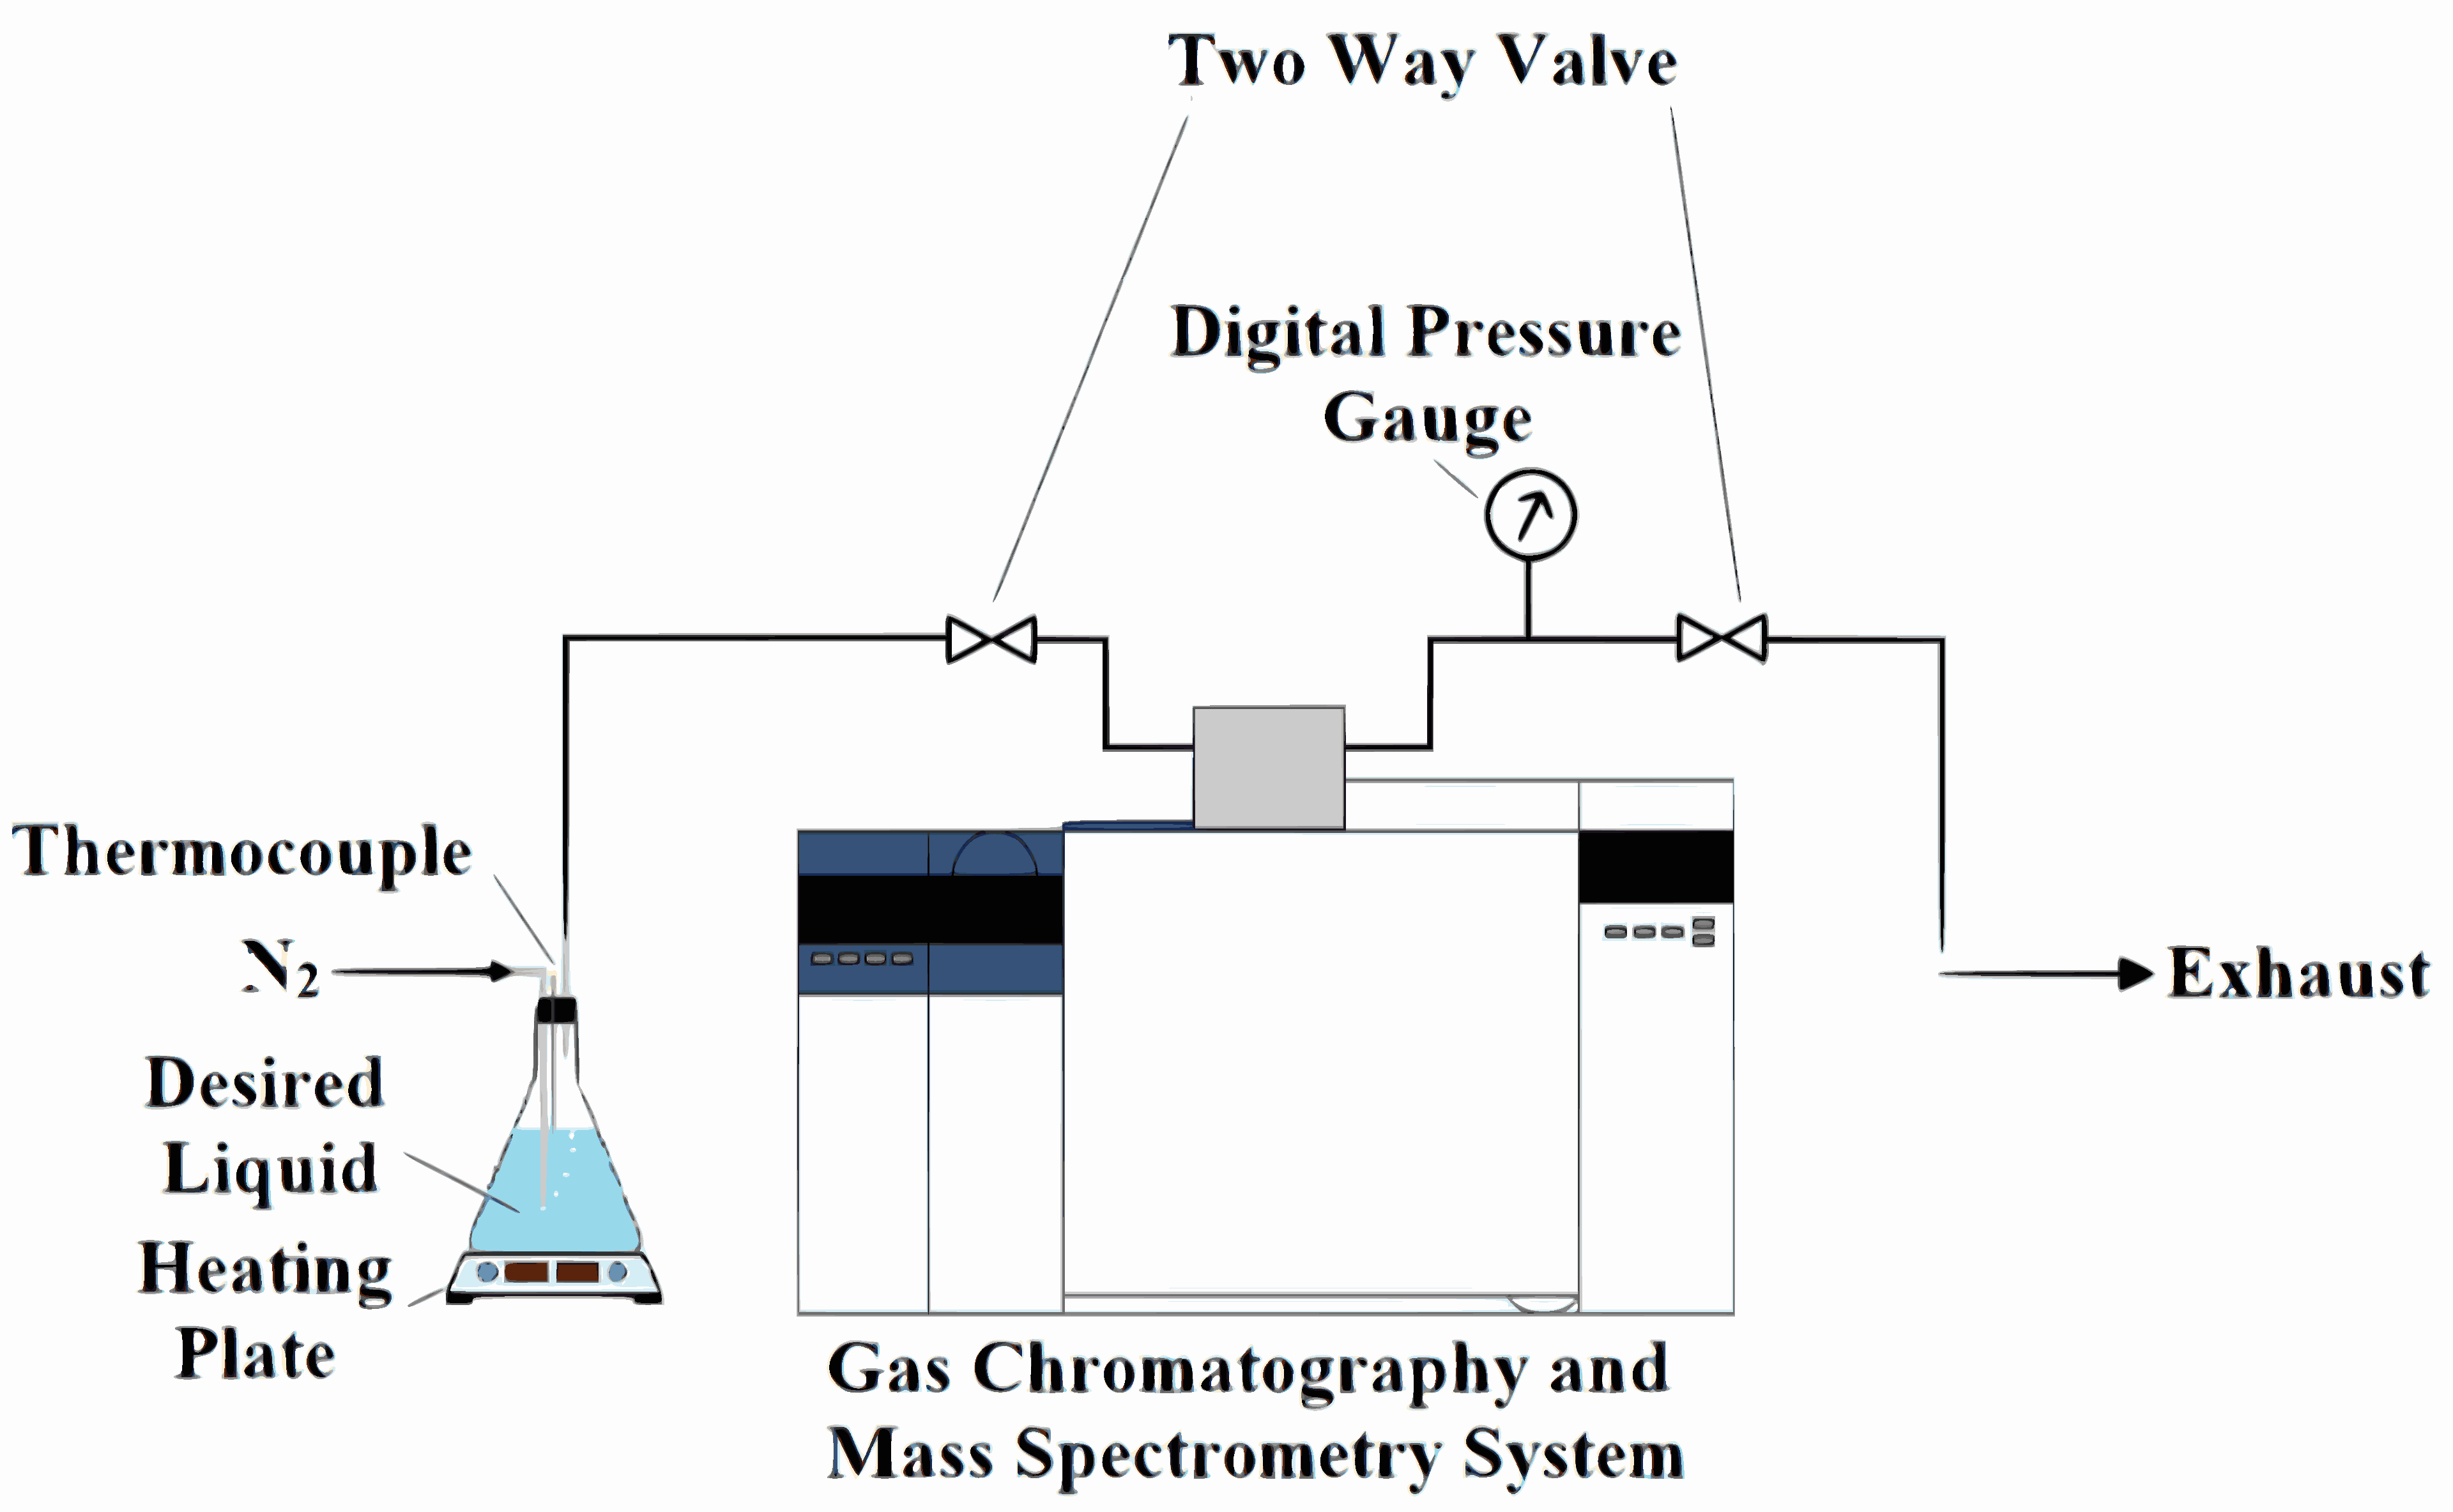
\includegraphics[width=\textwidth,keepaspectratio]{Bubbler_Setup.png}
	\caption[Flow diagram for bubble calibration system used for liquid materials]{Flow diagram for bubble calibration system used for liquid materials (acetone, ethanol, methanol, and water)}
	\label{fig:Bubbler}
\end{figure}
The material of interest is placed in a 500~ml Pyrex flask sitting on a heating plate. Nitrogen, acting as a carrier gas, is bubbled through the liquid bath and then transported through a heated gas line and into the GC/MS sample loop. Vapor from the liquid is transported along with the carrier gas in an amount liquid depending on the temperature. The concentration of the vapor injected into the GC/MS is calculated from a liquid-vapor pressure correlation provided by DIPPR~\cite{Dippr}.

\begin{equation}
\label{eq:liquid_vapor_pressure_correlation}
P_{\rm vap} ={\rm e}^{A+\frac{B}{T_{\rm B}}+C\,\ln{(T_{\rm B})}+D\,(T_{\rm B})^{E}}
\end{equation}
In this correlation, $P_{\rm vap}$ is the vapor pressure calculated from the temperature of the liquid bath, $T_{\rm B}$, with the coefficients ($A$, $B$, $C$, $D$, $E$) specific to the liquid material. Table~\ref{tab:Liquid Calibrate_Table} lists all coefficients for each calibrated liquid, including the uncertainty of their respective correlations, $u_{\rm corr}$.

\begin{table}[!]
\caption{Liquid vapor pressure correlation coefficients for various calibrated liquids}
\label{tab:Liquid Calibrate_Table}
\centering
	\footnotesize
	\begin{tabular}{lcccccc}
			\hline
%\\[0.0005cm]
\textbf{Liquid Material} &\textbf{A}& \textbf{B}& \textbf{C}&\textbf{D}&\textbf{E}&\textbf{Uncertainty(\%)}\\
\hline
\\[0.001cm]
Acetone	&	69.006	&	-5599.6	&	-7.0985	&	6.2237E-6	& 	2.00	&  3.00\\
Ethanol	&	73.304	&	-7122.3	&	-7.1424	&	2.8853E-6	& 	2.00	&  1.00\\
Methanol	&	82.718	&	-6904.5	&	-8.8622	&	7.4664E-6	& 	2.00	&  3.00\\
Water		&	73.649	&	-7258.2	&	-7.3037	&	4.1653E-6	& 	2.00	&  0.20\\
%\\[0.01cm]
\hline
\end{tabular}
\end{table}

The concentration range of each calibrated liquid is approximately 2~\% to 50~\%. Liquid bath temperatures are controlled using a heating plate positioned underneath the insulated bubbler. The temperature of the bath is measured using a K-type thermocouple placed at the liquid surface. The bath temperature measurements are sampled at \SI{2}{\hertz} for \SI{50}{s} simultaneously with pressure and temperature measurements of the GC/MS sample loop. Liquid-vapor calibrations are conducted once the bath reaches a steady-state temperature (approximately 1~h) and the nitrogen/vapor gas mixture has swept through the sample loop. Upon injection into the GC/MS, pressure and temperature measurements of the sample loop are made as described in Appendix~\ref{ssec:Total Moles Injected into the GC/MS for Calibation}.

The uncertainty of the concentration determined using Eq.~(\ref{eq:liquid_vapor_concentration}) is estimated using the law of propagation of uncertainty:
\begin{equation}
\label{eq:vapor_concentration_uncertainty}
u_{\scriptscriptstyle C_{\rm vap}} = \sqrt{{\left( \frac{\partial C_{\rm vap}}{\partial P}\,u_{\scriptscriptstyle P} \right) }^2+{\left(\frac{\partial C_{\rm vap}}{\partial P_{\rm vap}}\,u_{\scriptscriptstyle P_{\rm vap}}\right)}^2}
\end{equation}
The uncertainty of the pressure measured upon injected is calculated from Eq.~(\ref{eq:pressure_uncertainty}). The uncertainty of the vapor pressure is found by combining the propagated error of liquid bath temperature and the uncertainty in the correlation via quadrature:
\begin{equation}
\label{eq:vapor_pressure_uncertainty}
u_{\scriptscriptstyle P_{\rm vap}} = \sqrt{{\left(\frac{\partial P_{\rm vap}}{\partial T_{\rm B}}\,u_{\scriptscriptstyle T_{\rm B}} \right)}^2+{u_{\rm corr}}^2}
\end{equation}
The Type A evaluation of uncertainty of the liquid bath temperature readings is determined from the standard error of the temperature, $s_{T_{\rm B}}$ readings from the sampling period. The Type B evaluation of uncertainty for the liquid bath temperature is defined as the bias error source (\SI{1.5}{\degree C}) in the thermocouple, $u_{\rm inst}$. The combined uncertainty liquid bath temperature is determined via quadrature:
\begin{equation}
\label{eq:temp_bath_uncertainty}
u_{\scriptscriptstyle T_{\rm B}} = \sqrt{u_{\rm \scriptscriptstyle inst}^2 + s_{\scriptscriptstyle T_{\rm B}}^2}
\end{equation}

\pagebreak

\section{Uncertainty Analysis of the Soot Mass Fraction} \label{sec:Uncertainty_Soot_Frac}

The local soot mass fraction measurements, $Y_{\rm s}$, made at various heights above the fuel surface are calculated through a combination of Eqs.~(\ref{eq:soot_mass_frac}), (\ref{eq:total_mass}), and (\ref{eq:gas_density}):
\begin{equation}\label{eq:overall_soot_mass_frac}
Y_{\rm s}= \frac{m_{\rm s} \, V_{s}}{\dot{V} \, \Delta t \, m_{\rm tot}}\frac{T_{\rm \infty}}{T_{\rm g}}
\end{equation}
where $m_{\rm s}$ is the mass of soot collected on the PTFE filter and gun cleaning patches, $\dot{V}$ is the volumetric flow rate, $V_{s}$ is the volume of the sample loop, $m_{\rm tot}$ is the total mass of the gas sample detected in the TCD and TIC chromatograms, $T_{\rm \infty}/T_{\rm g}$ is the ratio of the internal gas flow temperature readings of the mass flow controller to the temperature of the probe, and $\Delta t$ is the total sampling time. The uncertainty of the measured soot mass fraction is estimated using the law of propagation of uncertainty after determining the soot mass fraction:
\begin{equation}
\label{eq:soot_mass_frac_uncertainty}
u_{\scriptscriptstyle Y_{\rm s}} = \sqrt{{\left(\frac{\partial Y_{\rm s}}{\partial m_{\rm s}}\,u_{\scriptscriptstyle m_{\rm s}} \right)}^2+{\left(\frac{\partial Y_{\rm s}}{\partial \dot{V} }\,u_{\scriptscriptstyle \dot{V}} \right)}^2+{\left(\frac{\partial Y_{\rm s}}{\partial m_{\rm tot}}\,u_{\scriptscriptstyle m_{\rm tot}} \right)}^2}
\end{equation}
The uncertainty of the temperature measurements is not accounted for since the uncertainty of the soot mass fraction is dominated by the remaining parameters uncertainties.

\subsection{Mass of Soot}
\label{ssec:Mass_of_Soot}

The mass of soot is determined from the difference in mass of the dried PTFE filter and gun cleaning patches before and 48~h after each experiment. The Type~A evaluation of standard uncertainty of the mass of soot, $m_{\rm s}$, is taken as the standard deviation, $s_{m_{\rm s}}$, of the measurements sampled three times before and after each test. The Type B evaluation of uncertainty, $u_{\rm inst}$, is determined from the instrumentation error sources of the scale and is found to be 1~\% of the reading. The Type A evaluation of uncertainty dominates; thus, the standard uncertainty is approximately the standard deviation of the multiple measurements:
\begin{equation}
\label{eq:soot_mass_uncertainty}
u_{\scriptscriptstyle m_{\rm s}}\approx s_{\scriptscriptstyle m_{\rm s}}
\end{equation}

\subsection{Mass Flow Controller Volumetric Flow Rate}
\label{ssec:Mass_Flow_Controller_Volumetric_Flow_Rate}

A mass flow controller is used to measure the volumetric flow rate, $\dot{V}$, within the gas sampling line. The Type A uncertainty is taken as the standard deviation of the flow measurements sampled at \SI{2}{Hz} during the sampling period which varies from \SI{12}{min} to \SI{25}{min} depending on the sampling location within the fire. The Type B sources of uncertainty consist of the calibration error, $u_{\rm cal}$, and the precision error sources at calibration conditions, $u_{\rm prec}$. The calibration error is given as 2~ml/min. The precision error is 0.8~\% of the reading plus 0.2~\% of the full scale (\SI{2}{L/min}). The combined uncertainty is calculated via quadrature:
\begin{equation}
\label{eq:volumetric_flow_uncertainty}
u_{\scriptscriptstyle \dot{V}} = \sqrt{u_{\rm \scriptscriptstyle prec}^2 + u_{\rm \scriptscriptstyle cal}^2 + s_{\scriptscriptstyle \dot{V}}^2}
\end{equation}

\subsection{Total Mass Identified}
\label{ssec:Total_Mass_Identified_into_GC/MS}
The total mass detected in the TCD and TIC chromatograms, $m_{\rm tot}$, is calculated:
\begin{equation}
\label{eq:total_mass_detected}
m_{\rm tot}=\sum_{n=1}^{N} n_{i}{\textrm{W}_{i}}
\end{equation}
where $n_{i}$ is the moles of species $i$ and ${\textrm{W}_{i}}$ is the molar mass.  The uncertainty in the total mass is calculated from the uncertainties of all identified species, defined in Section~\ref{ssec:Total Number of Moles Identified}, multiplied by their corresponding molar mass via quadrature:
\begin{equation}
\label{eq:total_mass_detected_uncertainty}
u_{\scriptscriptstyle m_{\rm tot}}=\sqrt{{\sum_{n=1}^{N} (u_{\scriptscriptstyle n_{i}}{\textrm{W}_{i}})^2}}
\end{equation}
where $N$ is the number of a species identified species in the chromatograms.

%\subsection{Mass Flow Controller Internal Gas Flow Temperature Reading}
%\label{ssec:MFC_Temp}

%The mass flow controller provides an internal gas flow temperature reading that is recorded manually during the gas sampling process. The uncertainty of the temperature reading is determined from the Type B evaluation of standard uncertainty of the mass flow controller temperature measurement defined as 0.75~\% of the reading.

%\subsection{The Effective Temperature of the Gas}
%\label{ssec:Probe_Temp}

%The uncertainty of the temperature measurements at the entrance of the probe is described in Appendix~\ref{sec:Uncertainty_Temperature_Measurements}.

\pagebreak

\section{Figures of Averaged Volume Fractions}\label{sec:Vol_Frac_Figs}

\subsection{Methanol}
\label{ssec:Methanol_ALL_Vol_Frac}
\begin{figure}[!h]
	\centering
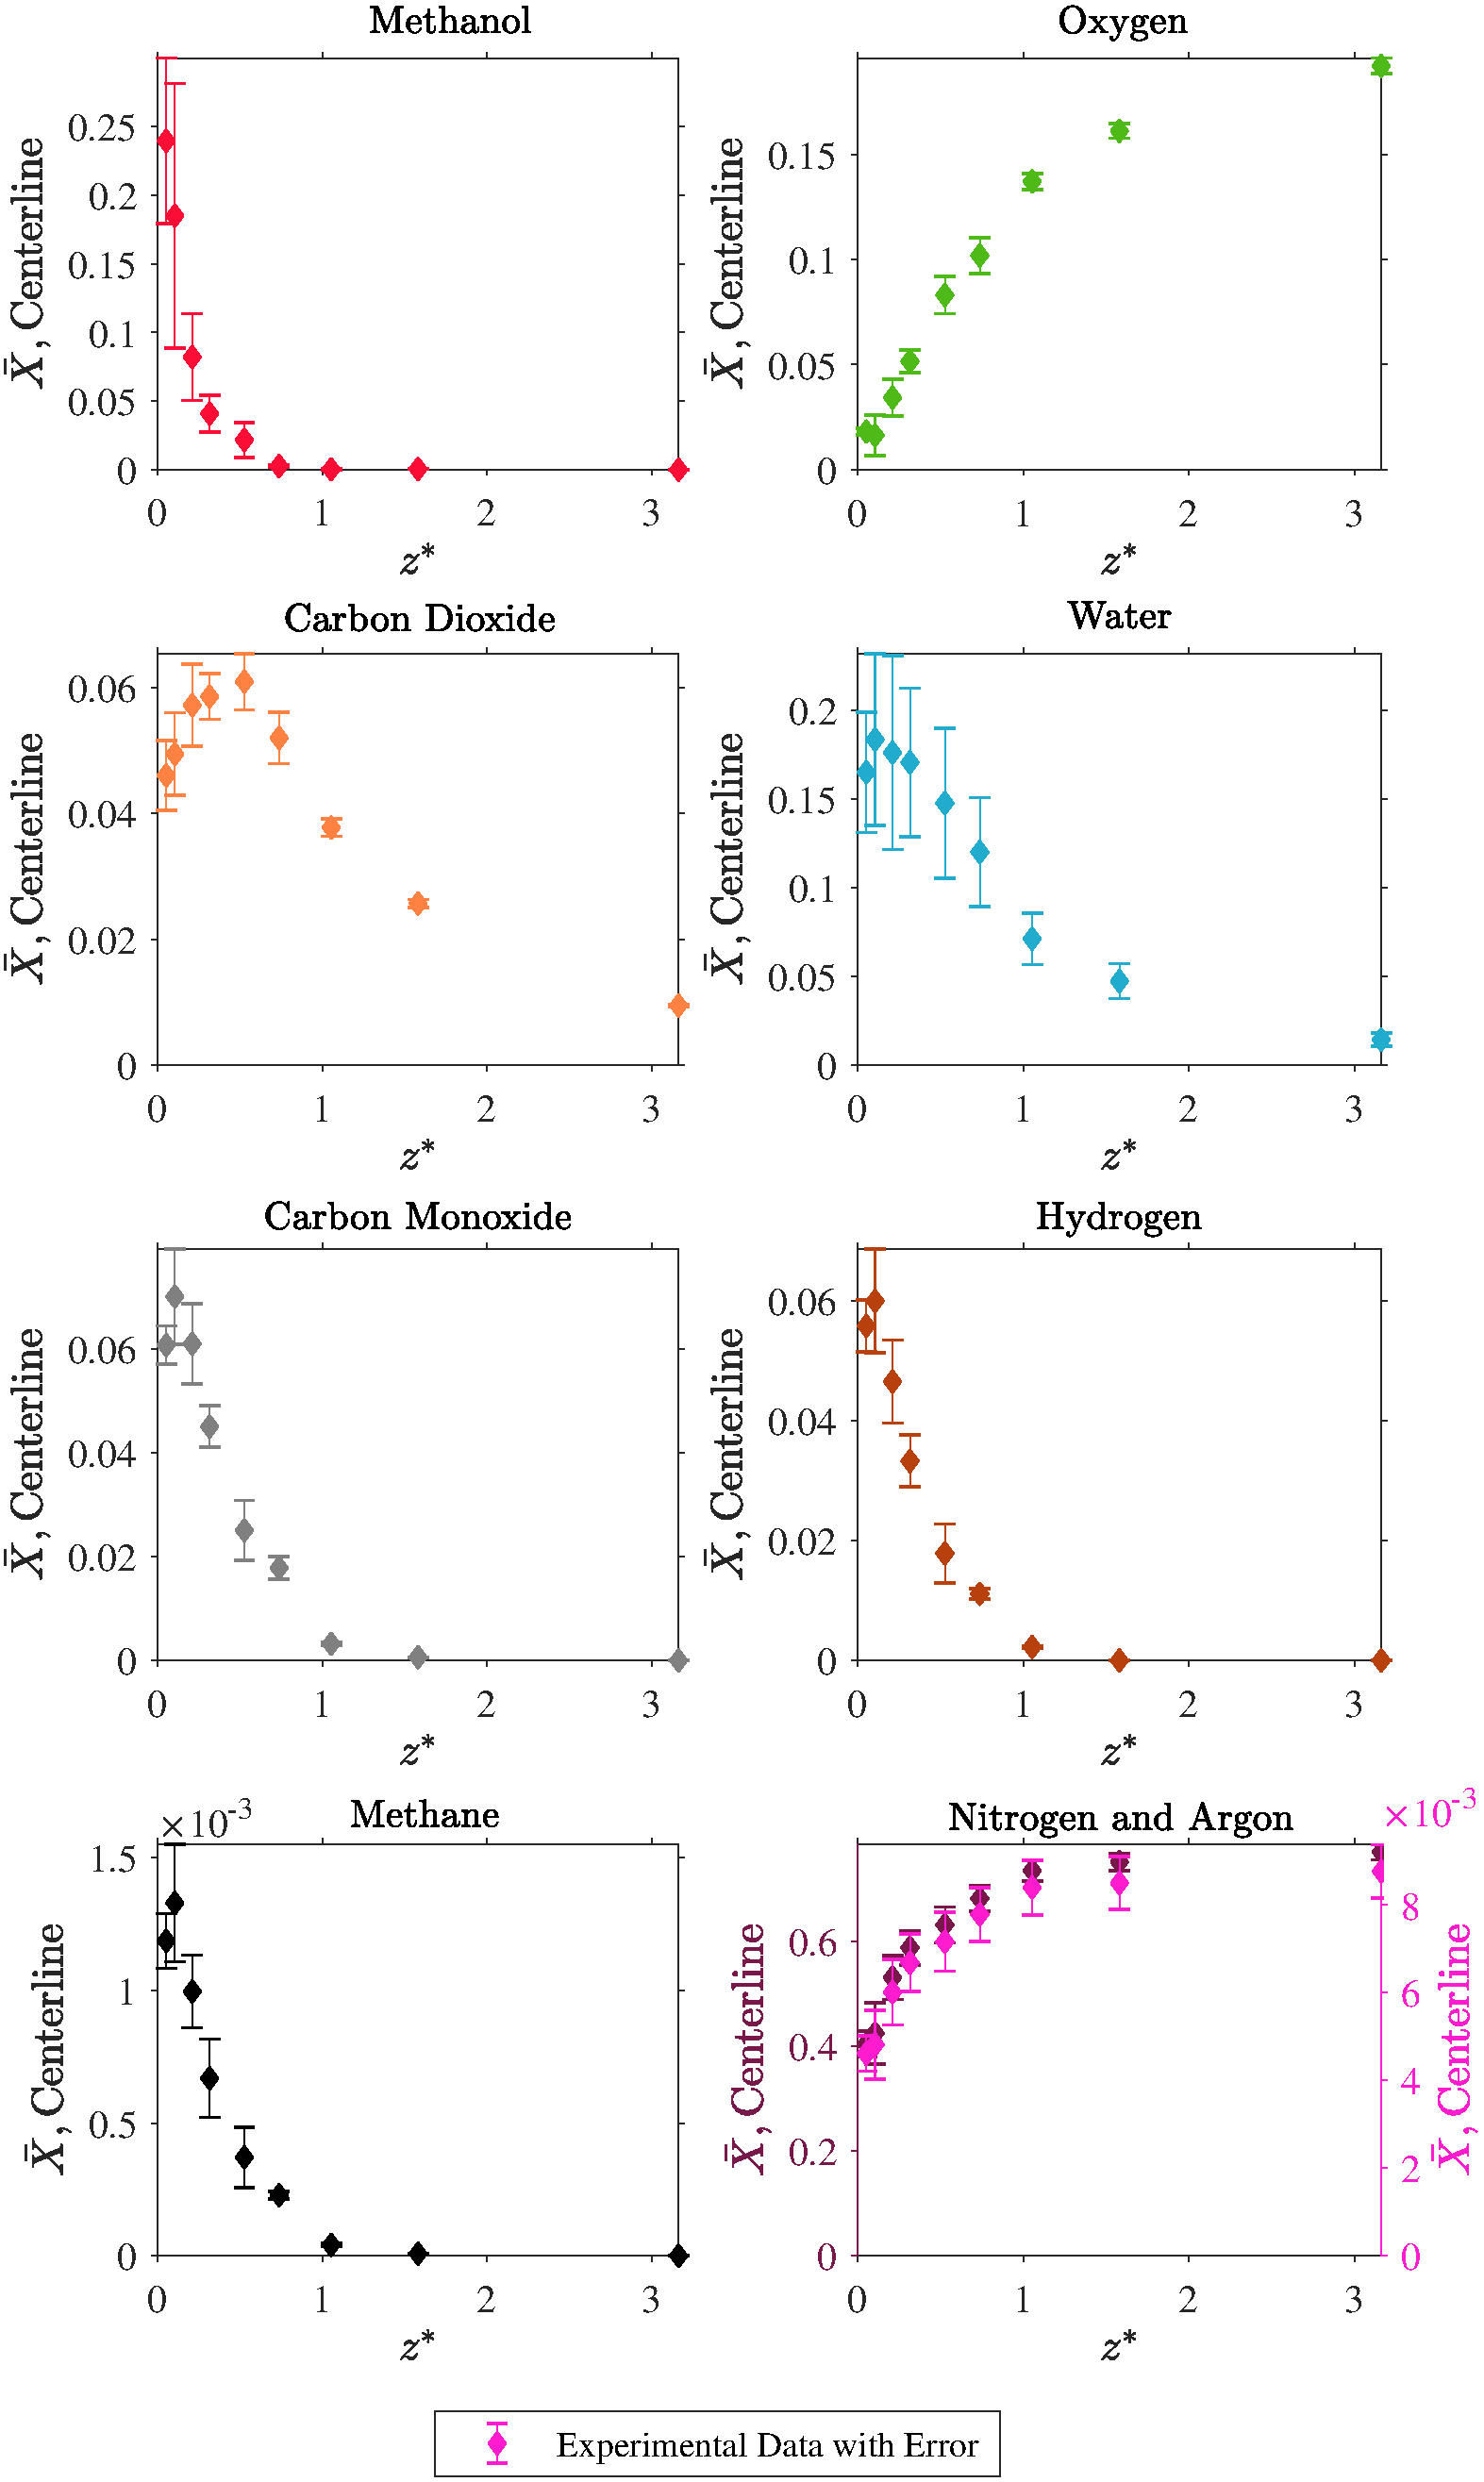
\includegraphics[width=10.75cm,keepaspectratio]{Methanol_MOL_FRAC_Plot_2.pdf}
	\caption[Volume fractions of major species in the methanol plume]{Plot of volume fractions of all species identified in the methanol pool fire as a function of $z^{*}$ along the pool centerline. The error is a combined uncertainty, further described in Section~\ref{sec:UncertaintyGasSpecies}.}
	\label{fig:Methanol_VOL_Frac_Major}
\end{figure}
\pagebreak

%\begin{figure}[!h]
%	\centering
%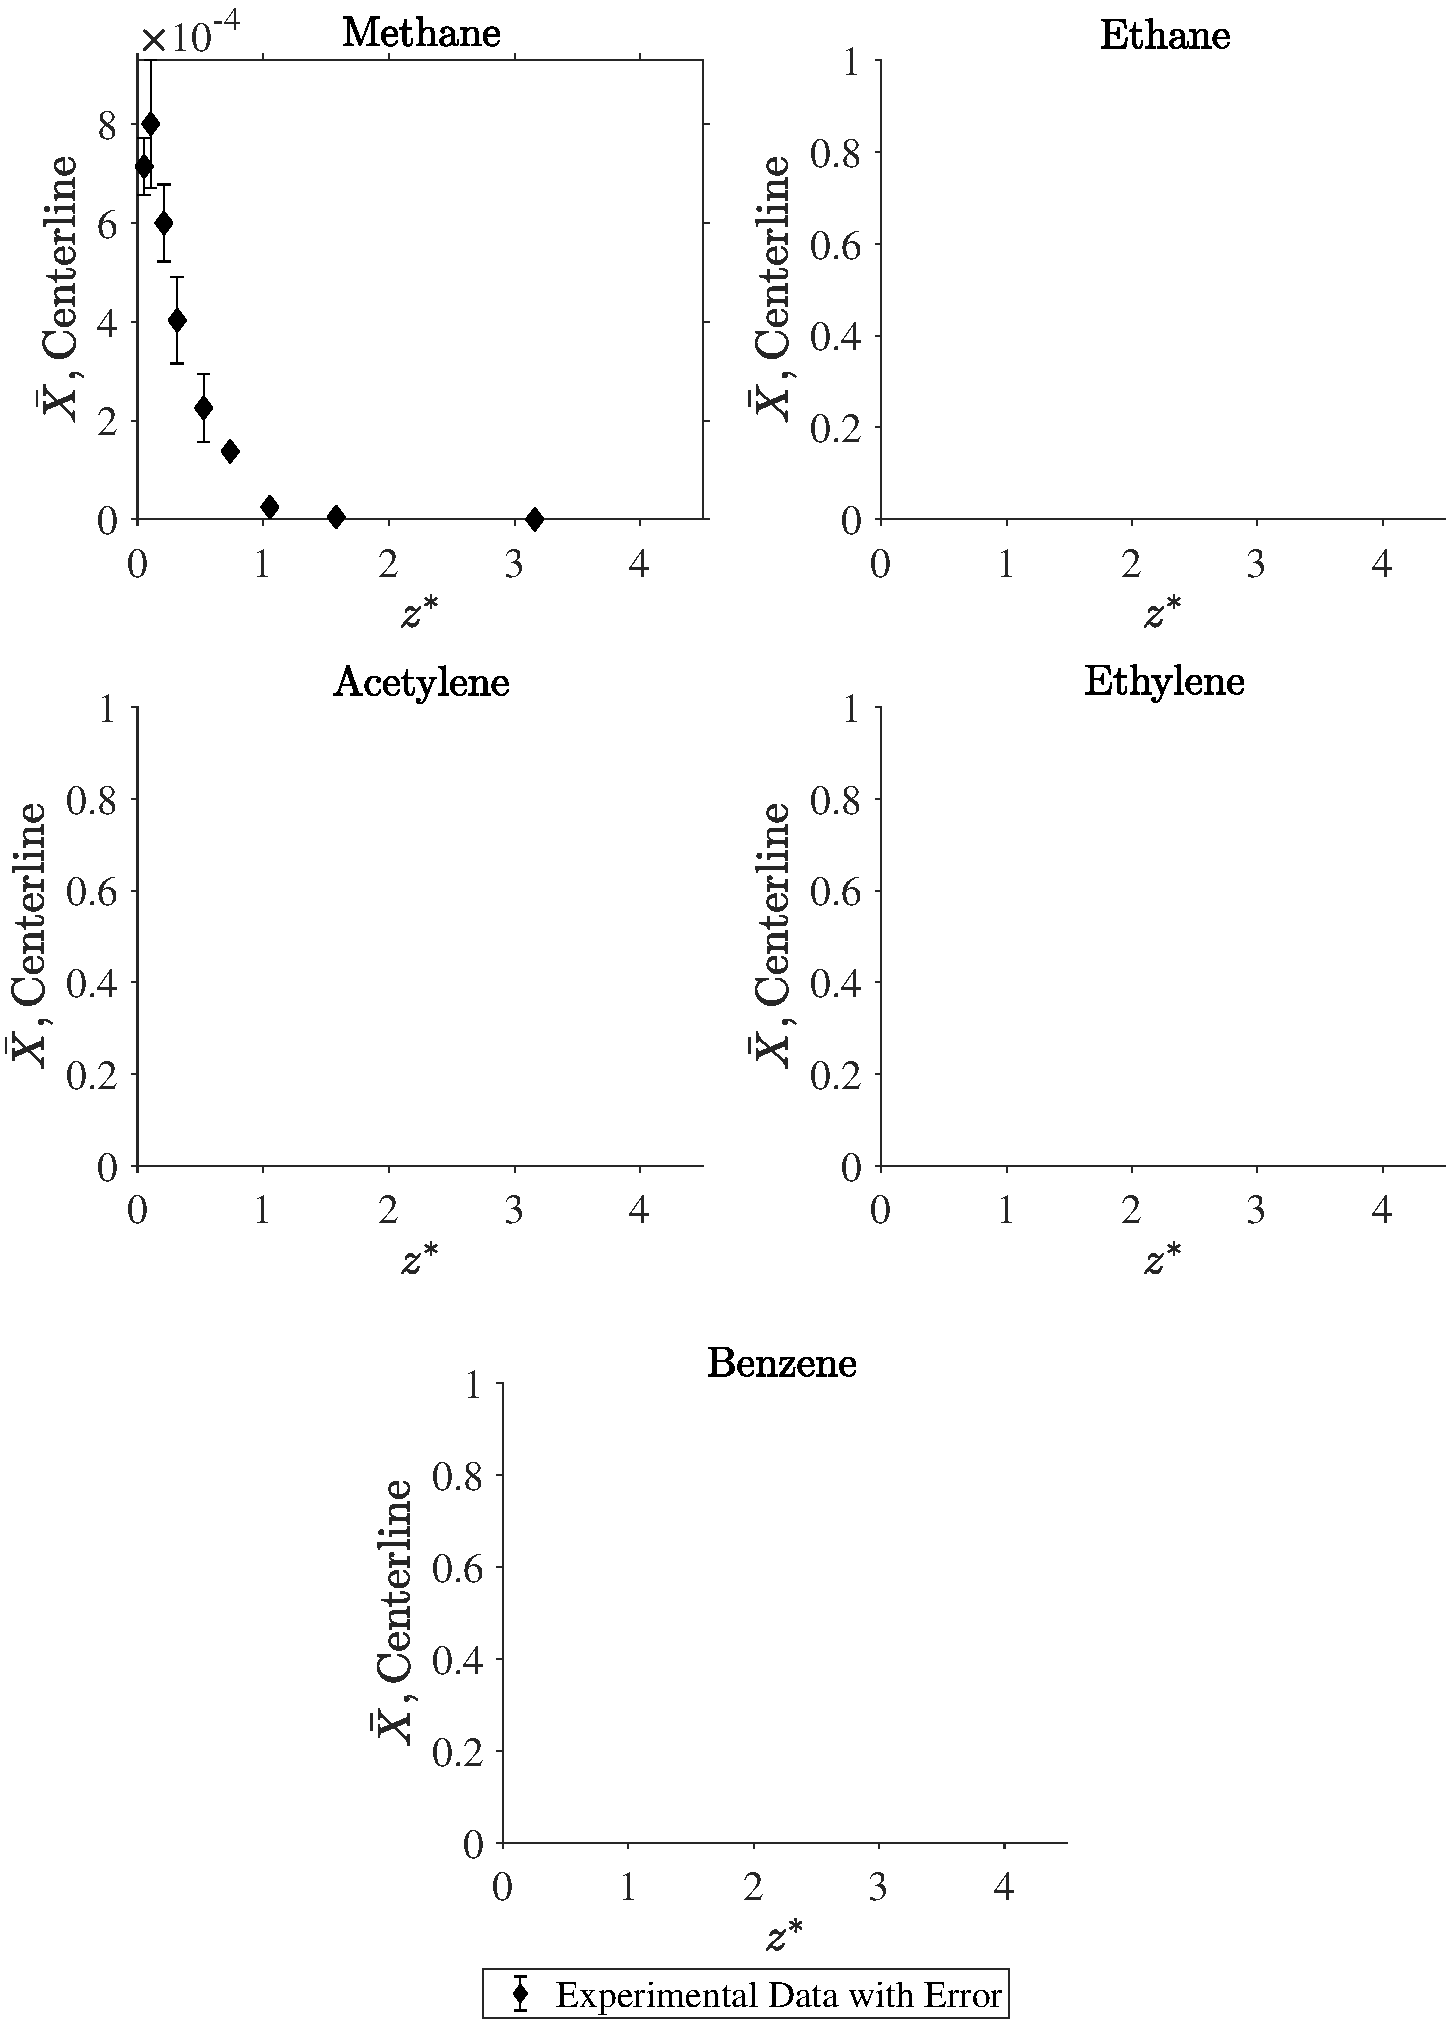
\includegraphics[width=10.75cm,keepaspectratio]{Methanol_Inter_MOL_FRAC_Plot.pdf}
%	\caption[Volume fractions of intermediate species in the methanol plume]{Plot of volume fractions of intermediate species identified in the methanol pool fire centerline as function of $z^{*}$}
%	\label{fig:Methanol_VOL_Frac_Inter}
%\end{figure}
%\pagebreak

\subsection{Ethanol}
\label{ssec:Ethanol_ALL_Vol_Frac}

\begin{figure}[!h]
	\centering
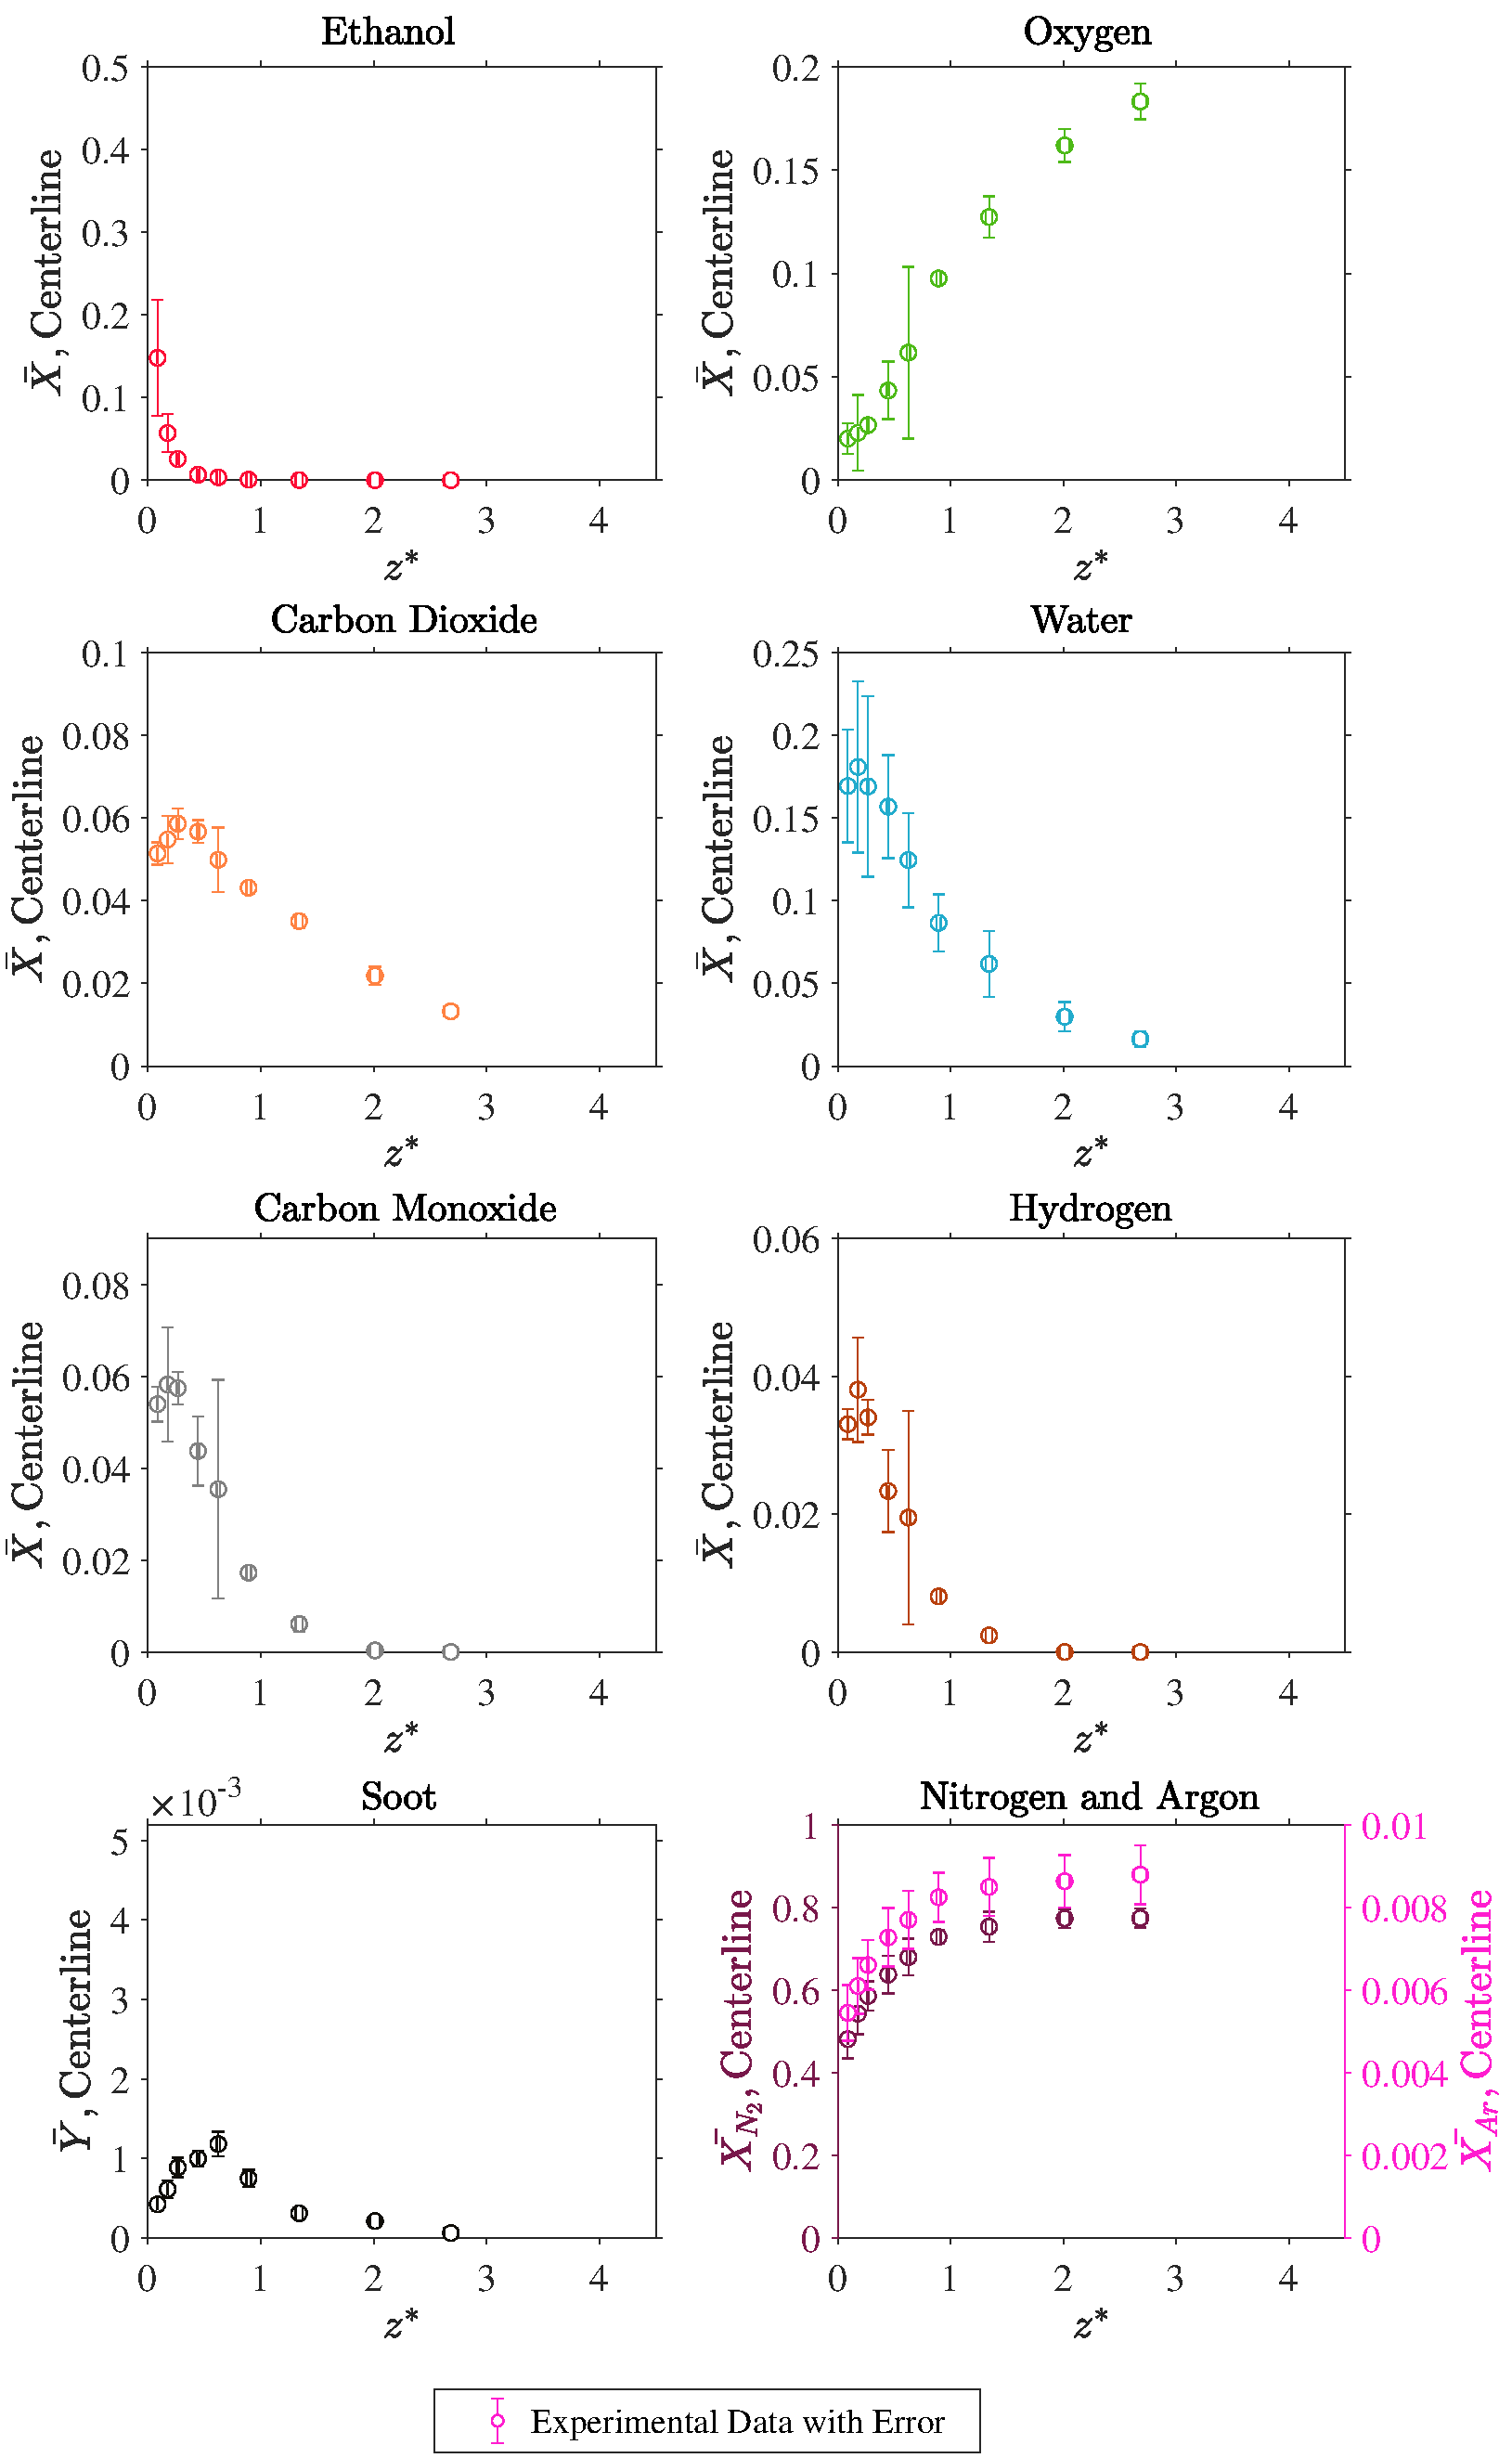
\includegraphics[width=10.75cm,keepaspectratio]{Ethanol_MOL_FRAC_Plot.pdf}
	\caption[Volume fractions of major species in the ethanol plume]{Plot of volume fractions of major species identified in the ethanol pool fire as a function of $z^{*}$ along the pool centerline. The error is a combined uncertainty, further described in Section~\ref{sec:UncertaintyGasSpecies}.}
	\label{fig:Ethanol_VOL_Frac_Major}
\end{figure}
\pagebreak

\begin{figure}[!h]
	\centering
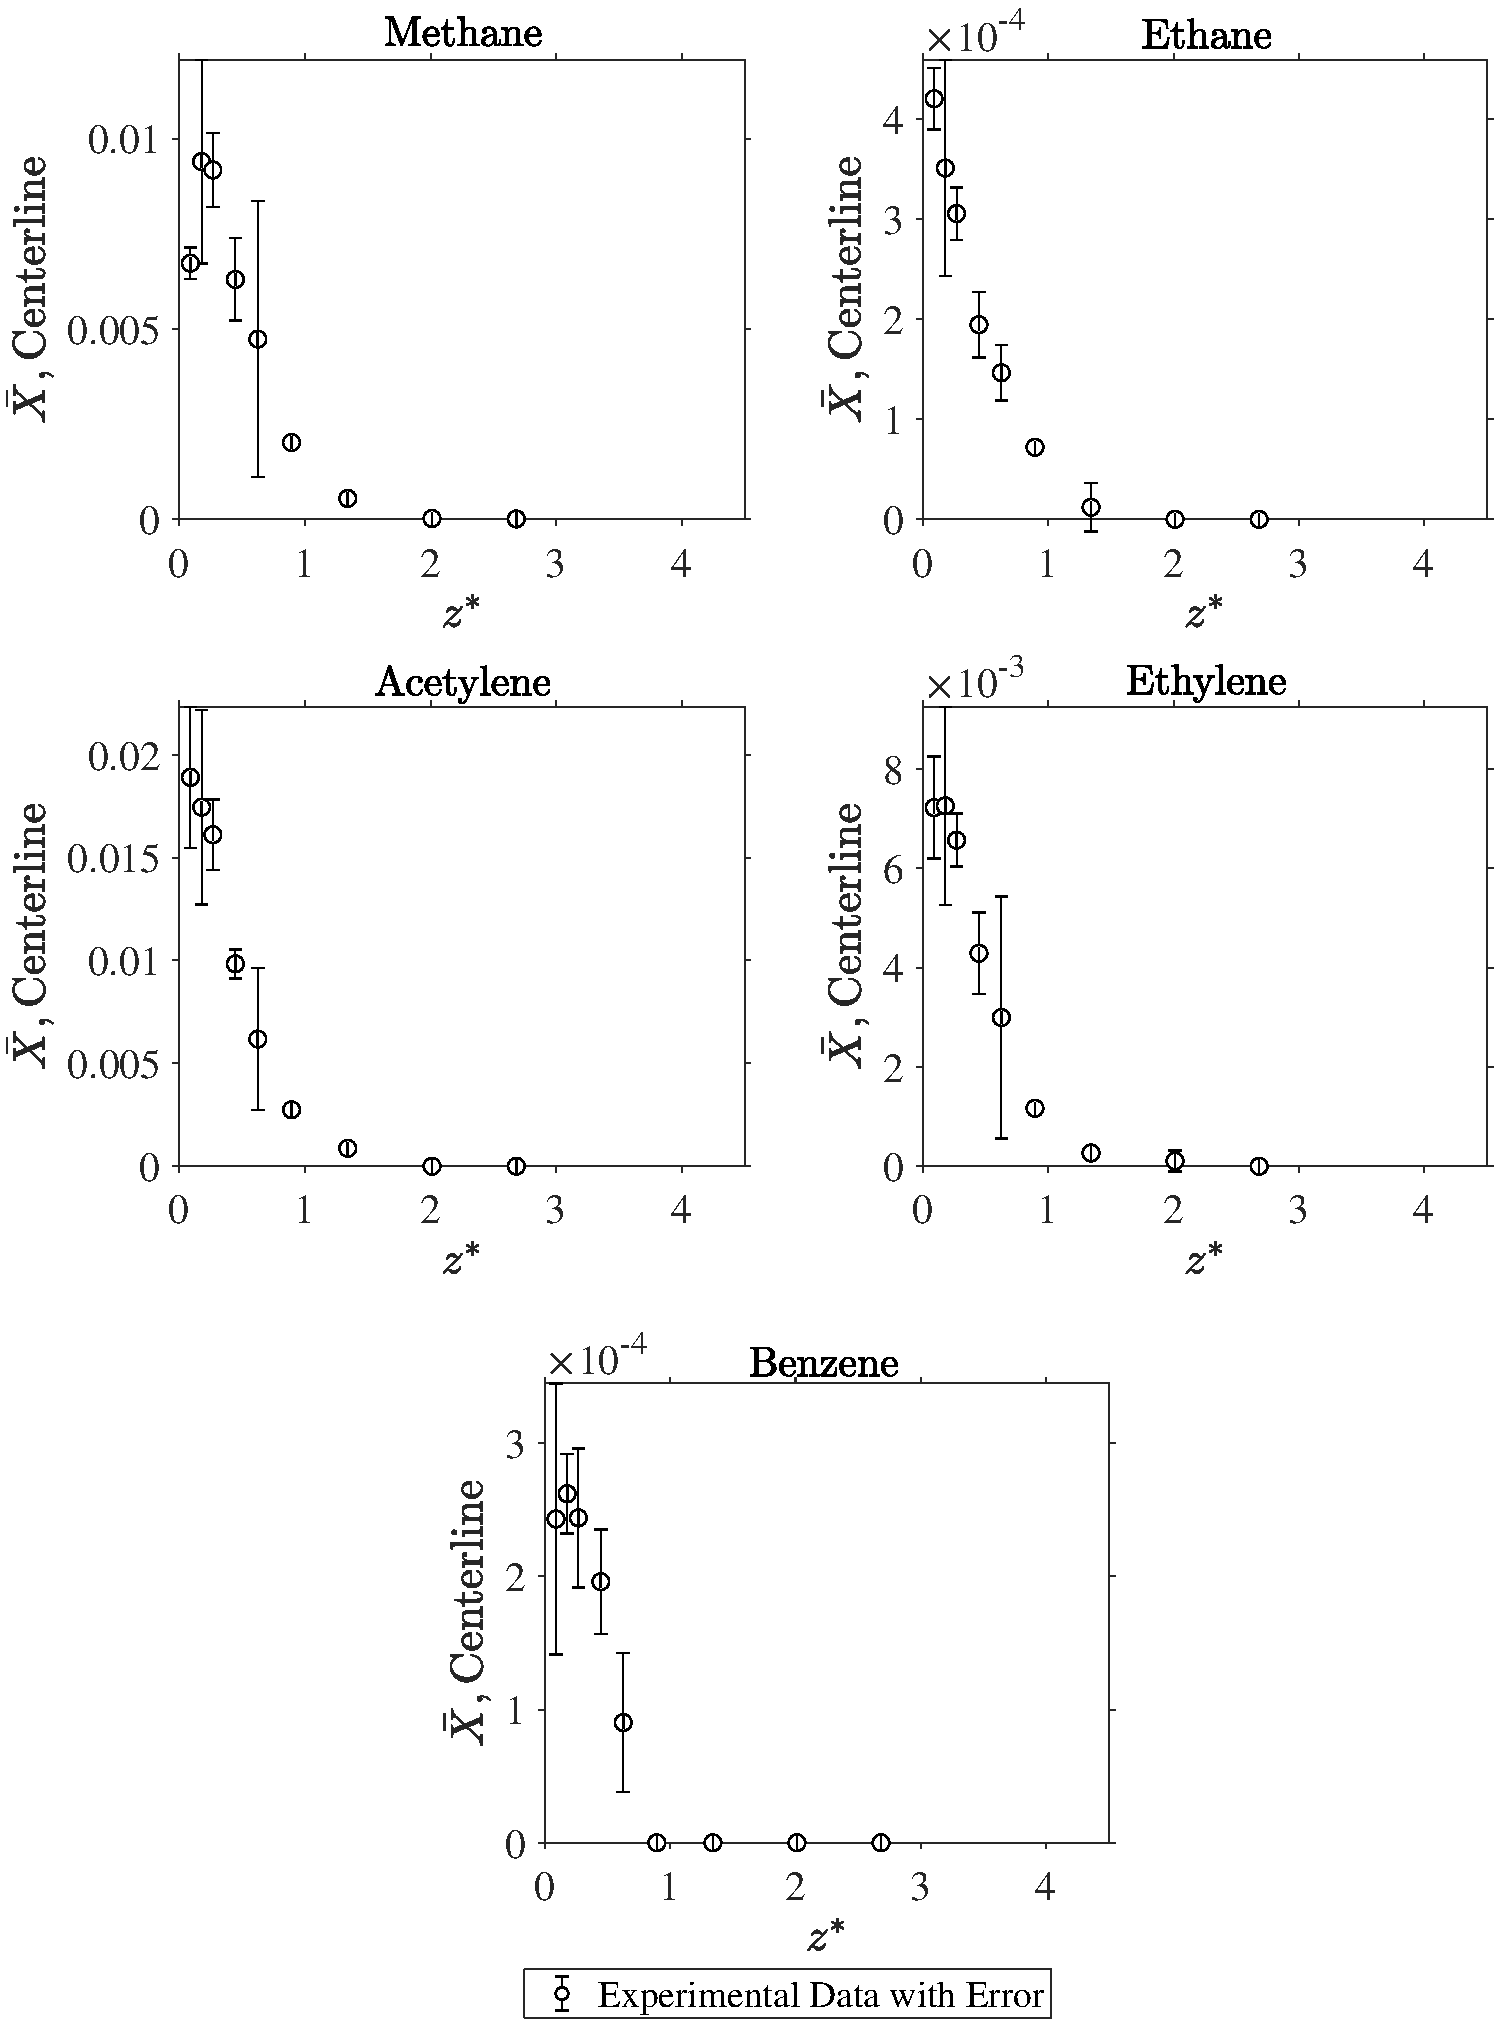
\includegraphics[width=10.75cm,keepaspectratio]{Ethanol_Inter_MOL_FRAC_Plot.pdf}
	\caption[Volume fractions of minor and trace species in the ethanol plume]{Plot of volume fractions of minor and trace species identified in the ethanol pool fire as a function of $z^{*}$ along the pool centerline. The error is a combined uncertainty, further described in Section~\ref{sec:UncertaintyGasSpecies}.}
	\label{fig:Ethanol_VOL_Frac_Inter}
\end{figure}

\clearpage
\subsection{Acetone}
\label{ssec:Acetonel_ALL_Vol_Frac}

\begin{figure}[!h]
	\centering
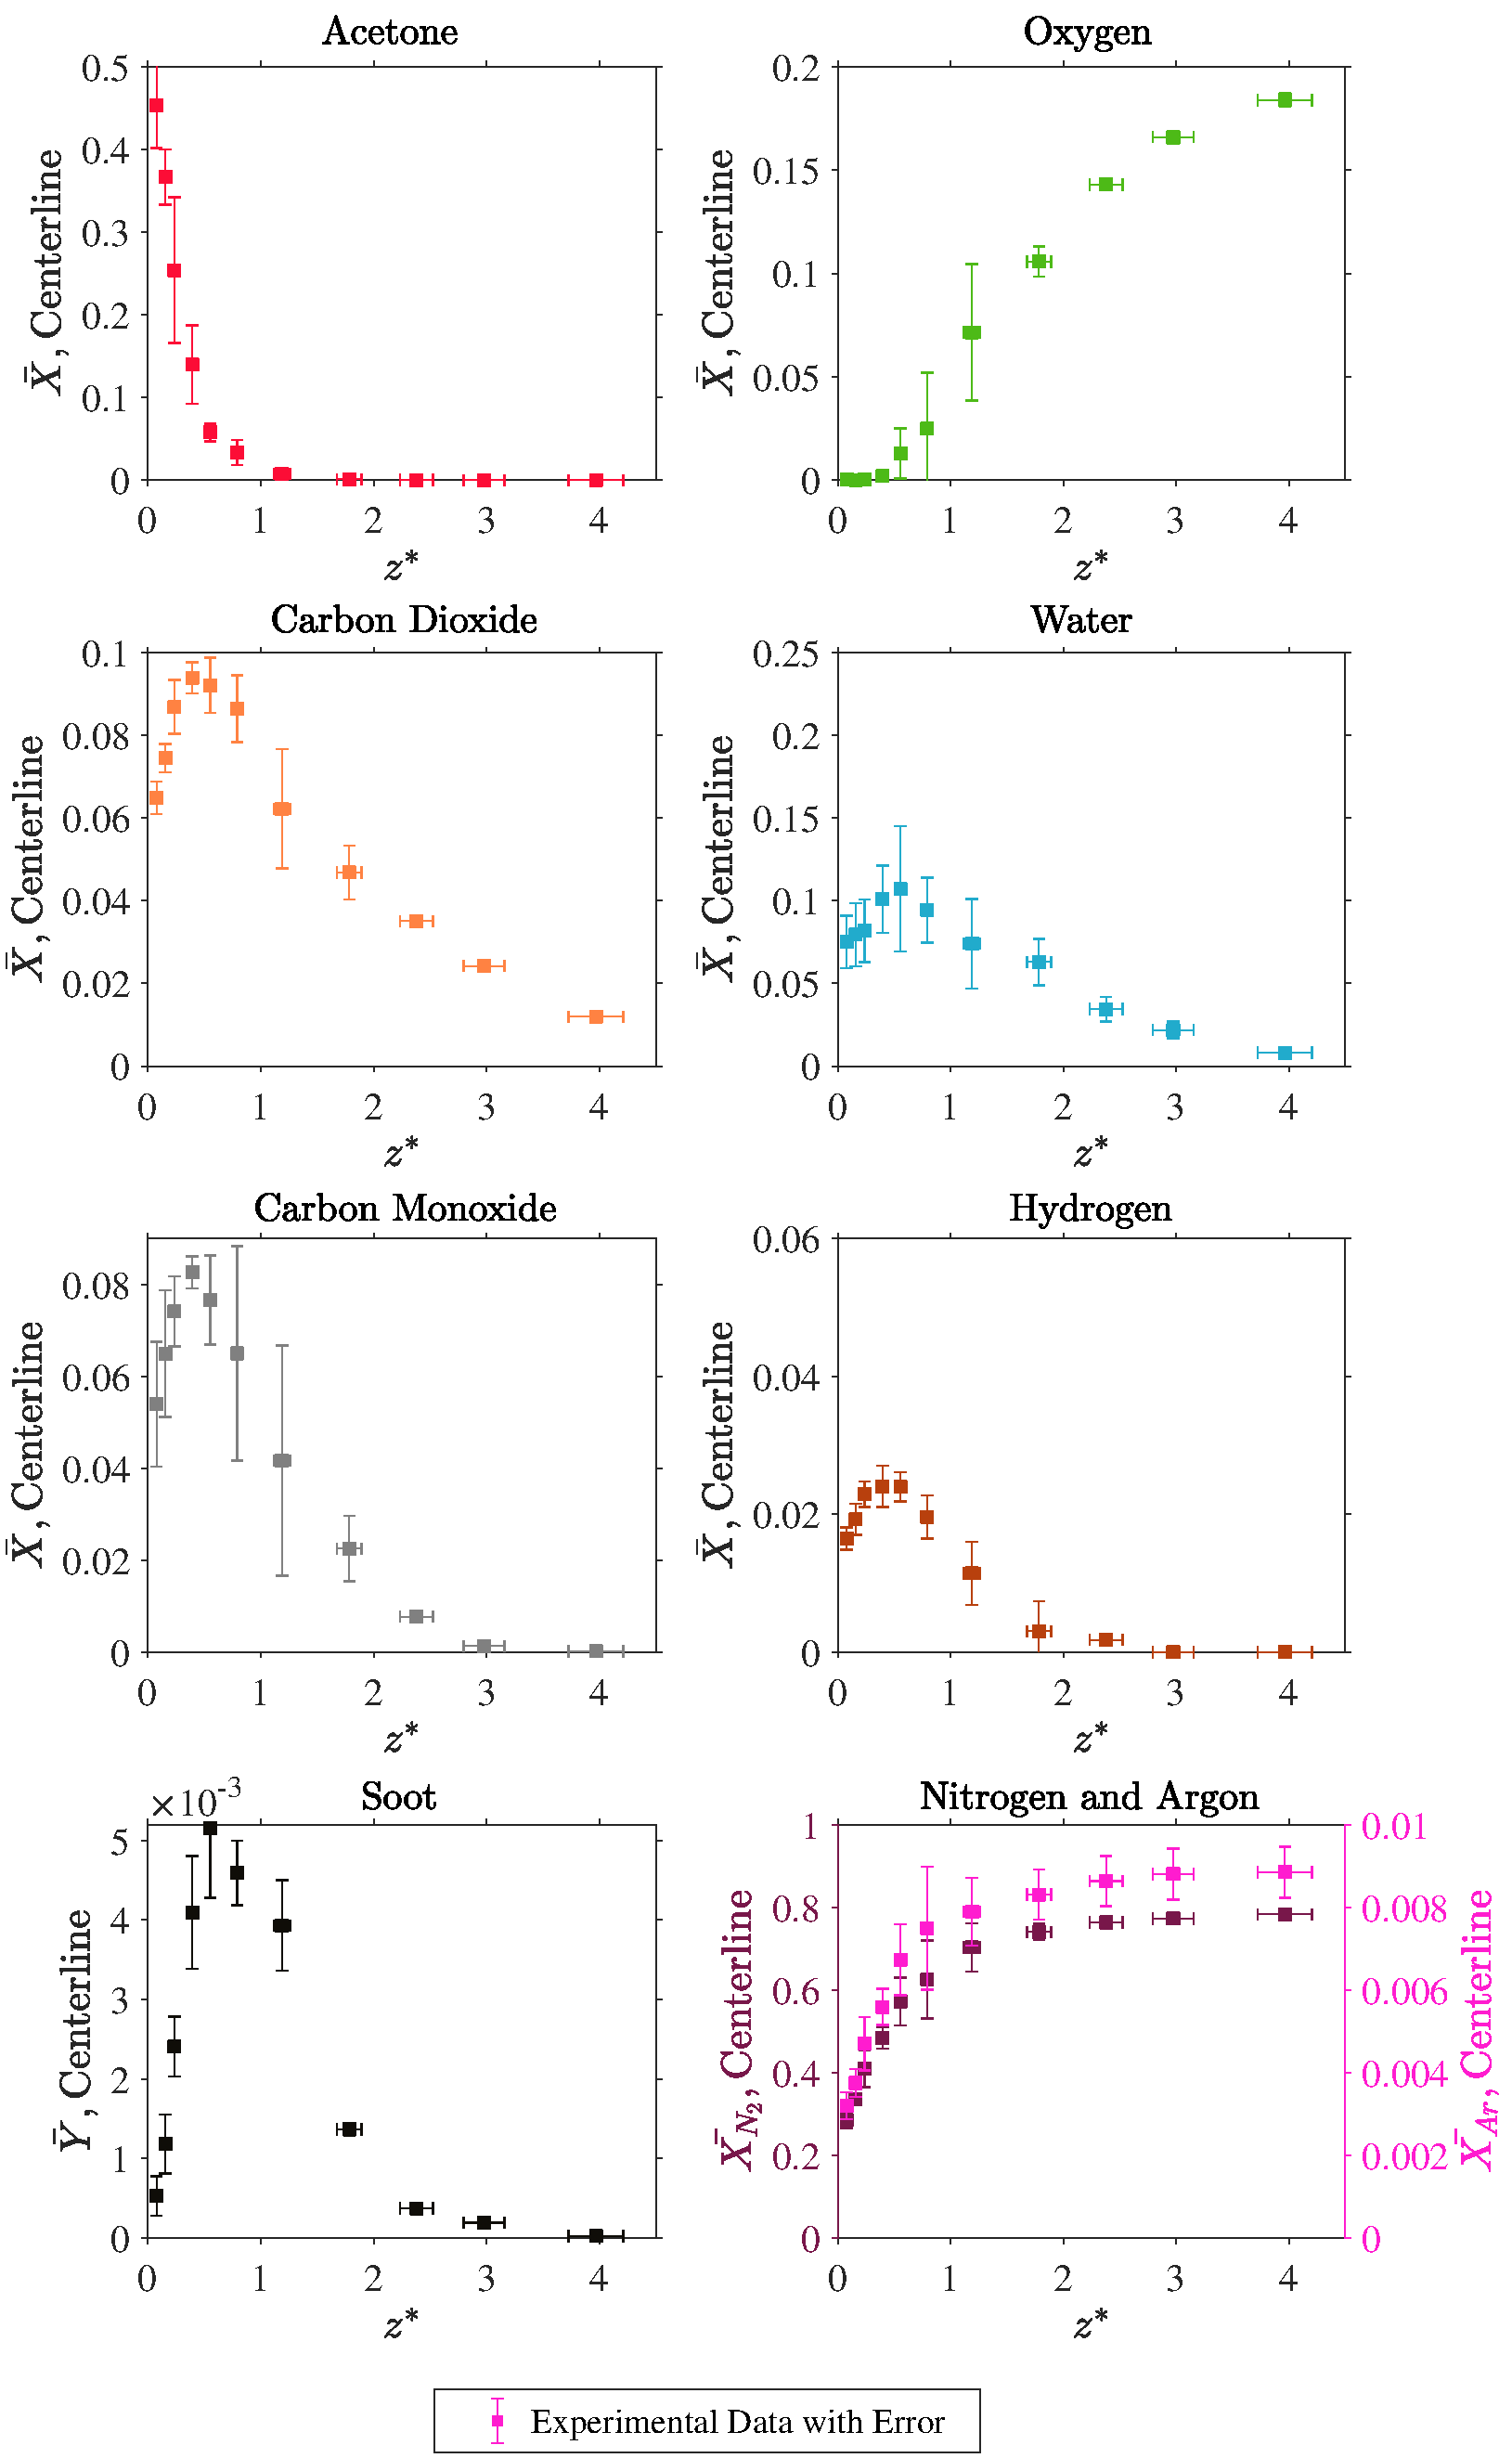
\includegraphics[width=10.75cm,keepaspectratio]{Acetone_MOL_FRAC_Plot.pdf}
	\caption[Volume fractions of major species in the acetone plume]{Plot of volume fractions of major species identified in the acetone pool fire as a function of $z^{*}$ along the pool centerline. The error is a combined uncertainty, further described in Section~\ref{sec:UncertaintyGasSpecies}.}
	\label{fig:Acetone_VOL_Frac_Major}
\end{figure}

\begin{figure}[!h]
	\centering
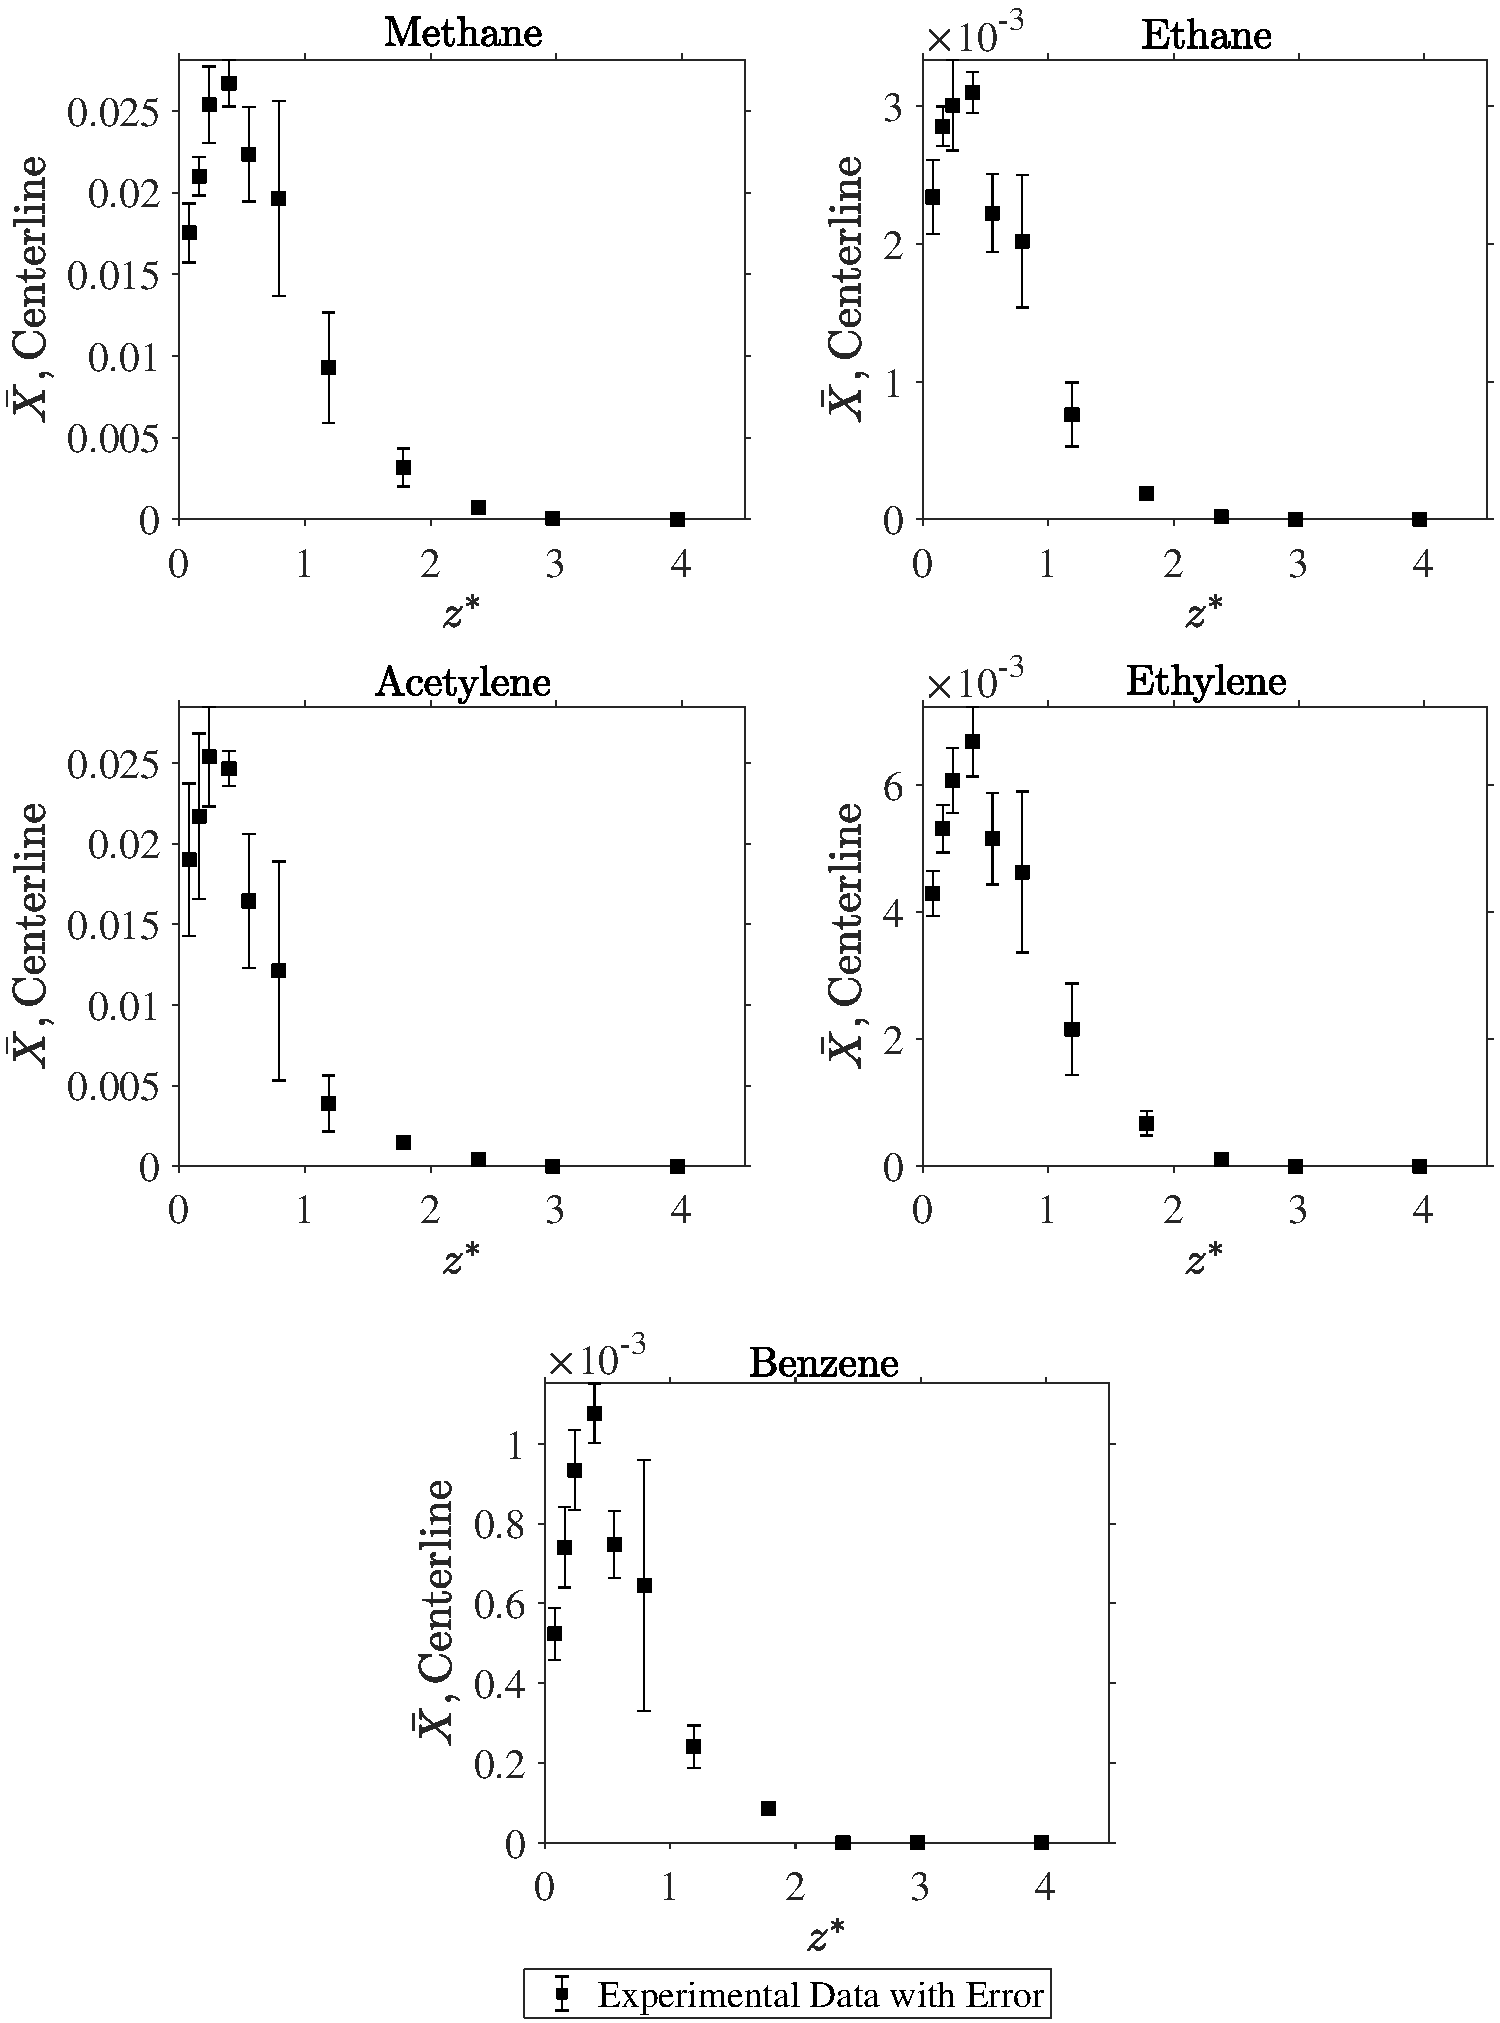
\includegraphics[width=10.75cm,keepaspectratio]{Acetone_Inter_MOL_FRAC_Plot.pdf}
	\caption[Volume fractions of minor and trace species in the acetone plume]{Plot of volume fractions of minor and trace species identified in the acetone pool fire as a function of $z^{*}$ along the pool centerline. The error is a combined uncertainty, further described in Section~\ref{sec:UncertaintyGasSpecies}.}
	\label{fig:Acetone_VOL_Frac_Inter}
\end{figure}

\clearpage
\subsection{Methane}
\label{ssec:Methane_ALL_Vol_Frac}
\begin{figure}[!h]
	\centering
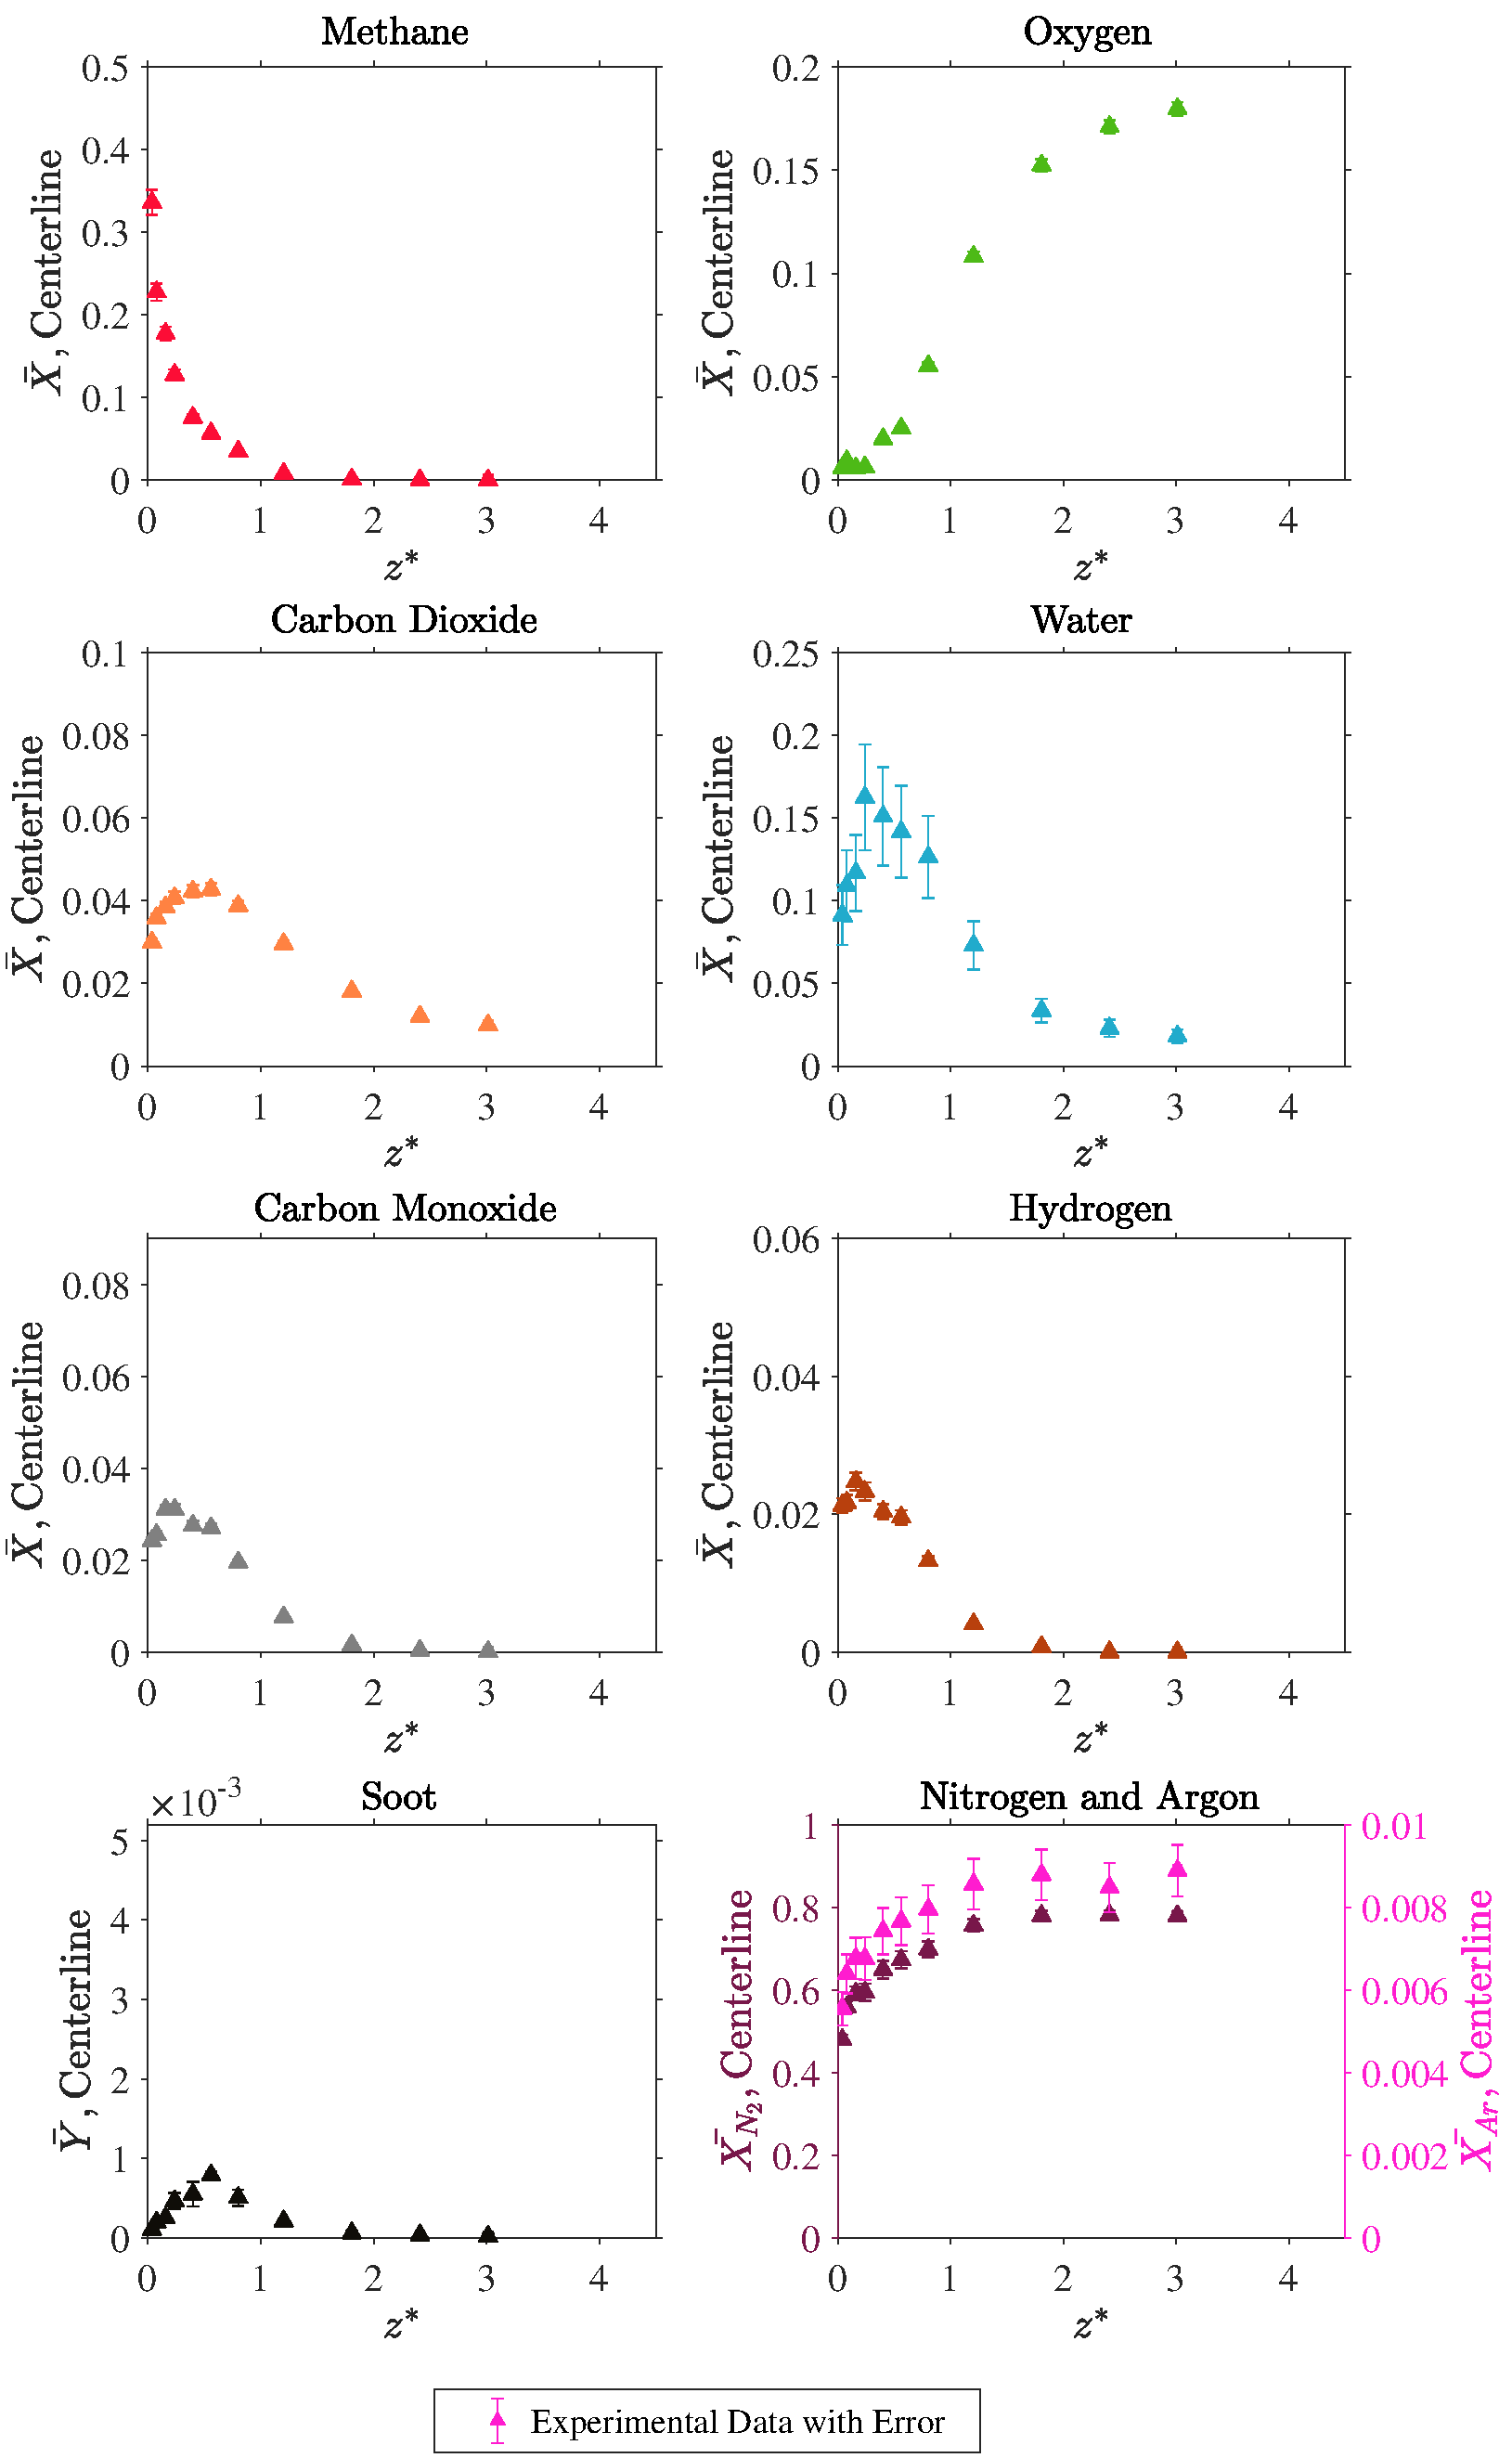
\includegraphics[width=10.75cm,keepaspectratio]{Methane_MOL_FRAC_Plot.pdf}
	\caption[Volume fractions of major species in the methane plume]{Plot of volume fractions of all species identified in the methane pool fire as a function of $z^{*}$ along the pool centerline. The error is a combined uncertainty, further described in Section~\ref{sec:UncertaintyGasSpecies}.}
	\label{fig:Methane_VOL_Frac_Major}
\end{figure}

\begin{figure}[!h]
	\centering
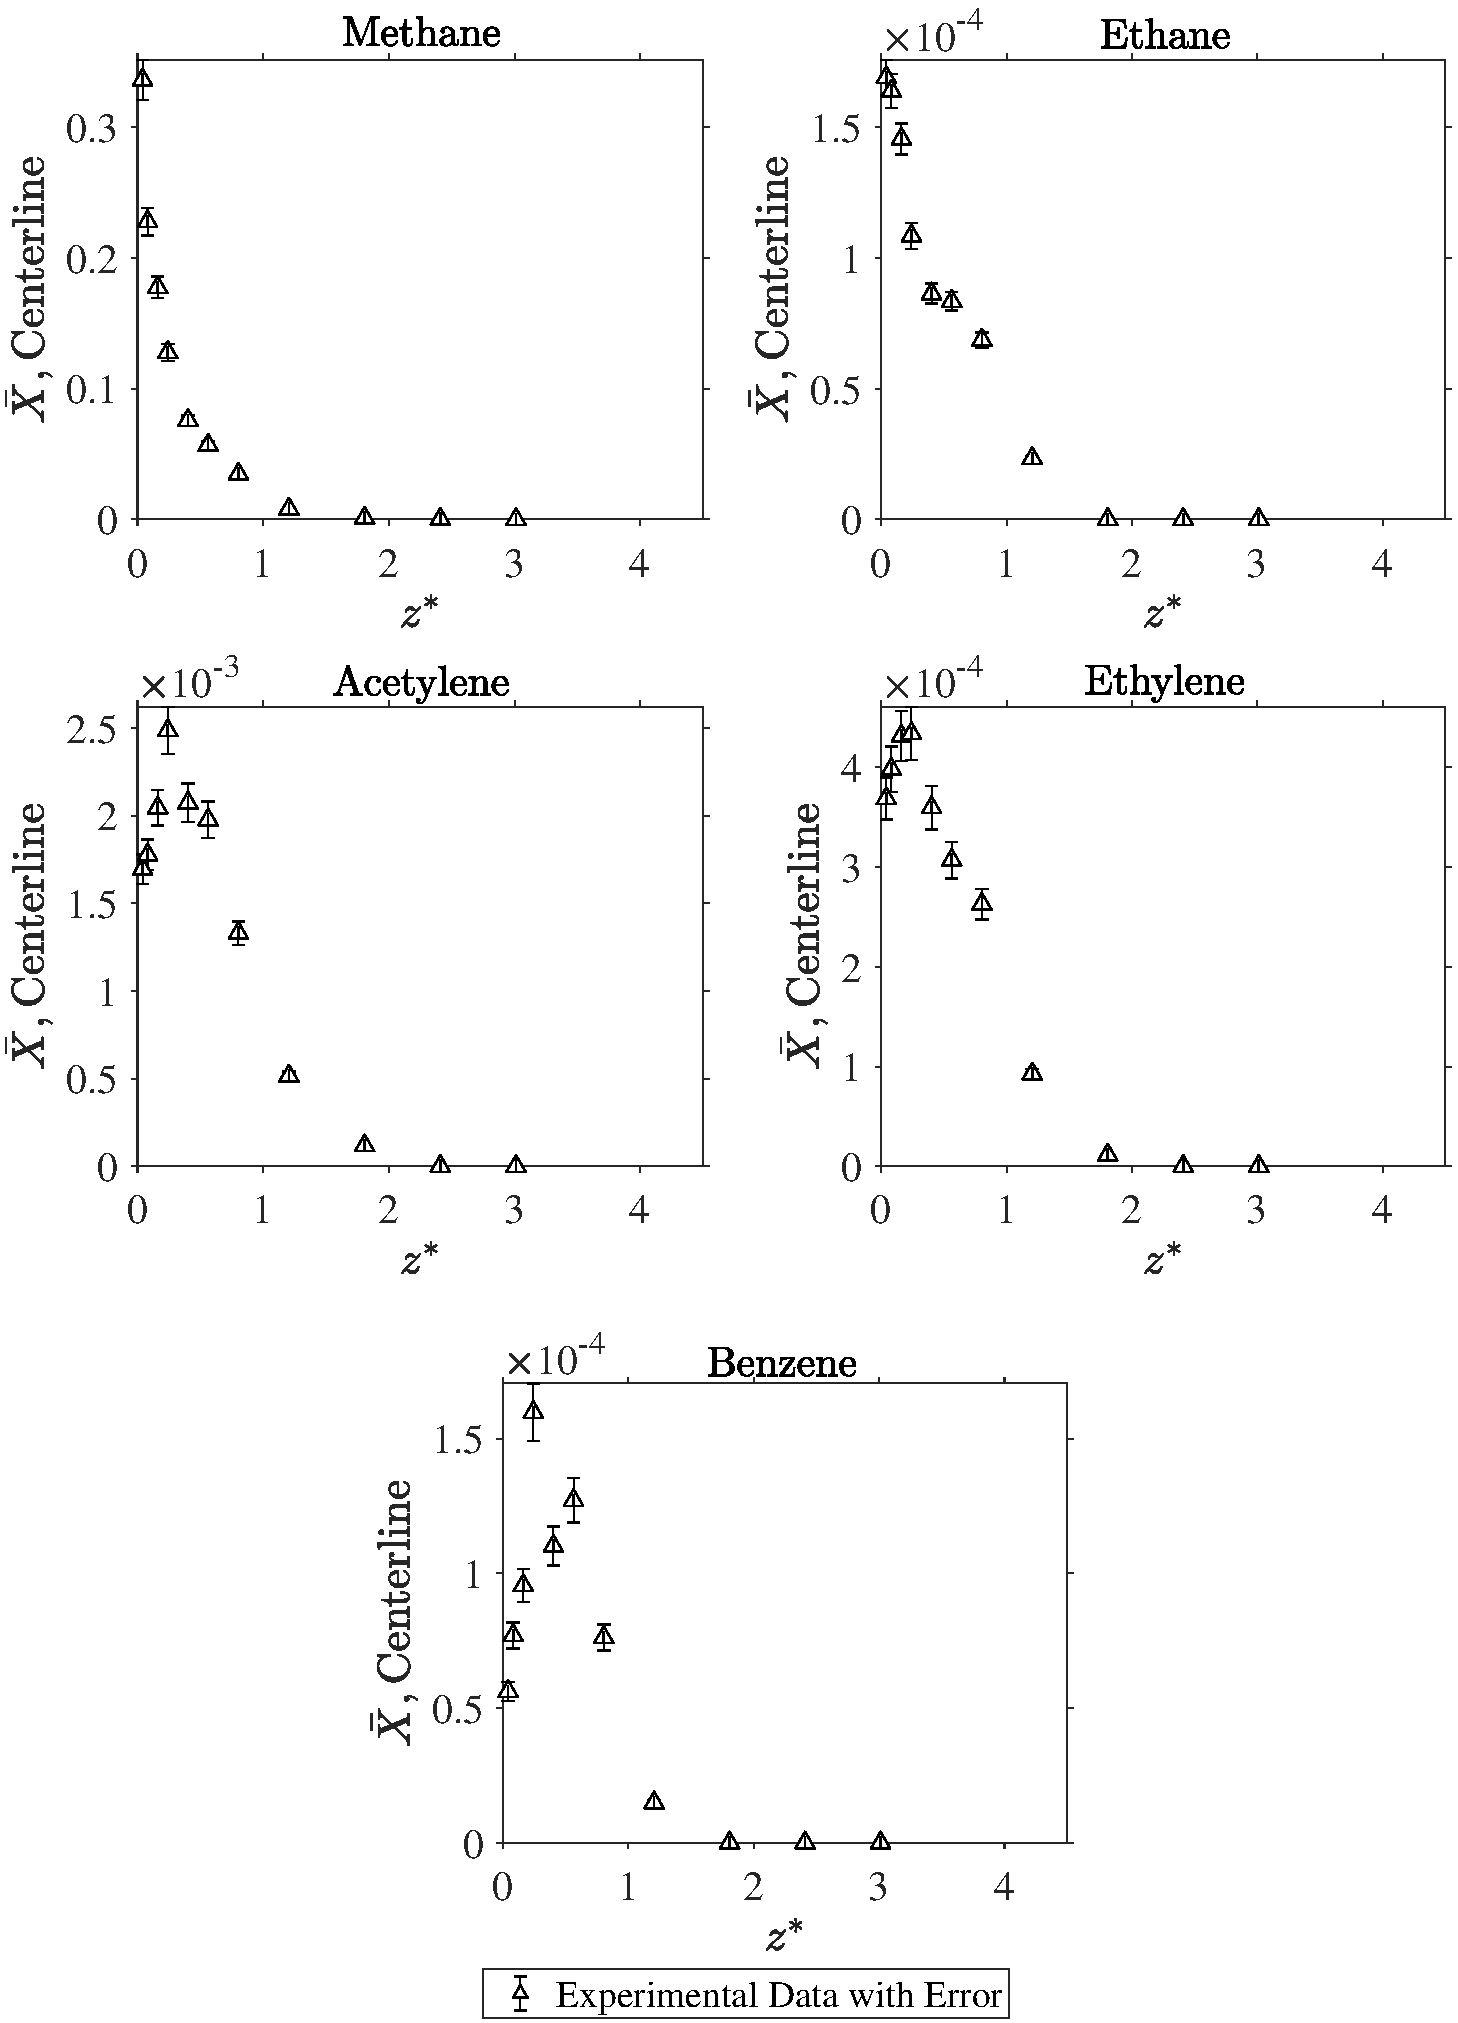
\includegraphics[width=10.75cm,keepaspectratio]{Methane_Inter_MOL_FRAC_Plot.pdf}
	\caption[Volume fractions of minor and trace species in the methane plume]{Plot of volume fractions of minor and trace species identified in the methane pool fire as a function of $z^{*}$ along the pool centerline. The error presented here is a combined uncertainty, further described in Section~\ref{sec:UncertaintyGasSpecies}.}
	\label{fig:Methane_VOL_Frac_Inter}
\end{figure}

\pagebreak
\subsection{Propane (20 kW)}
\label{ssec:Propane20kW_ALL_Vol_Frac}
\begin{figure}[!h]
	\centering
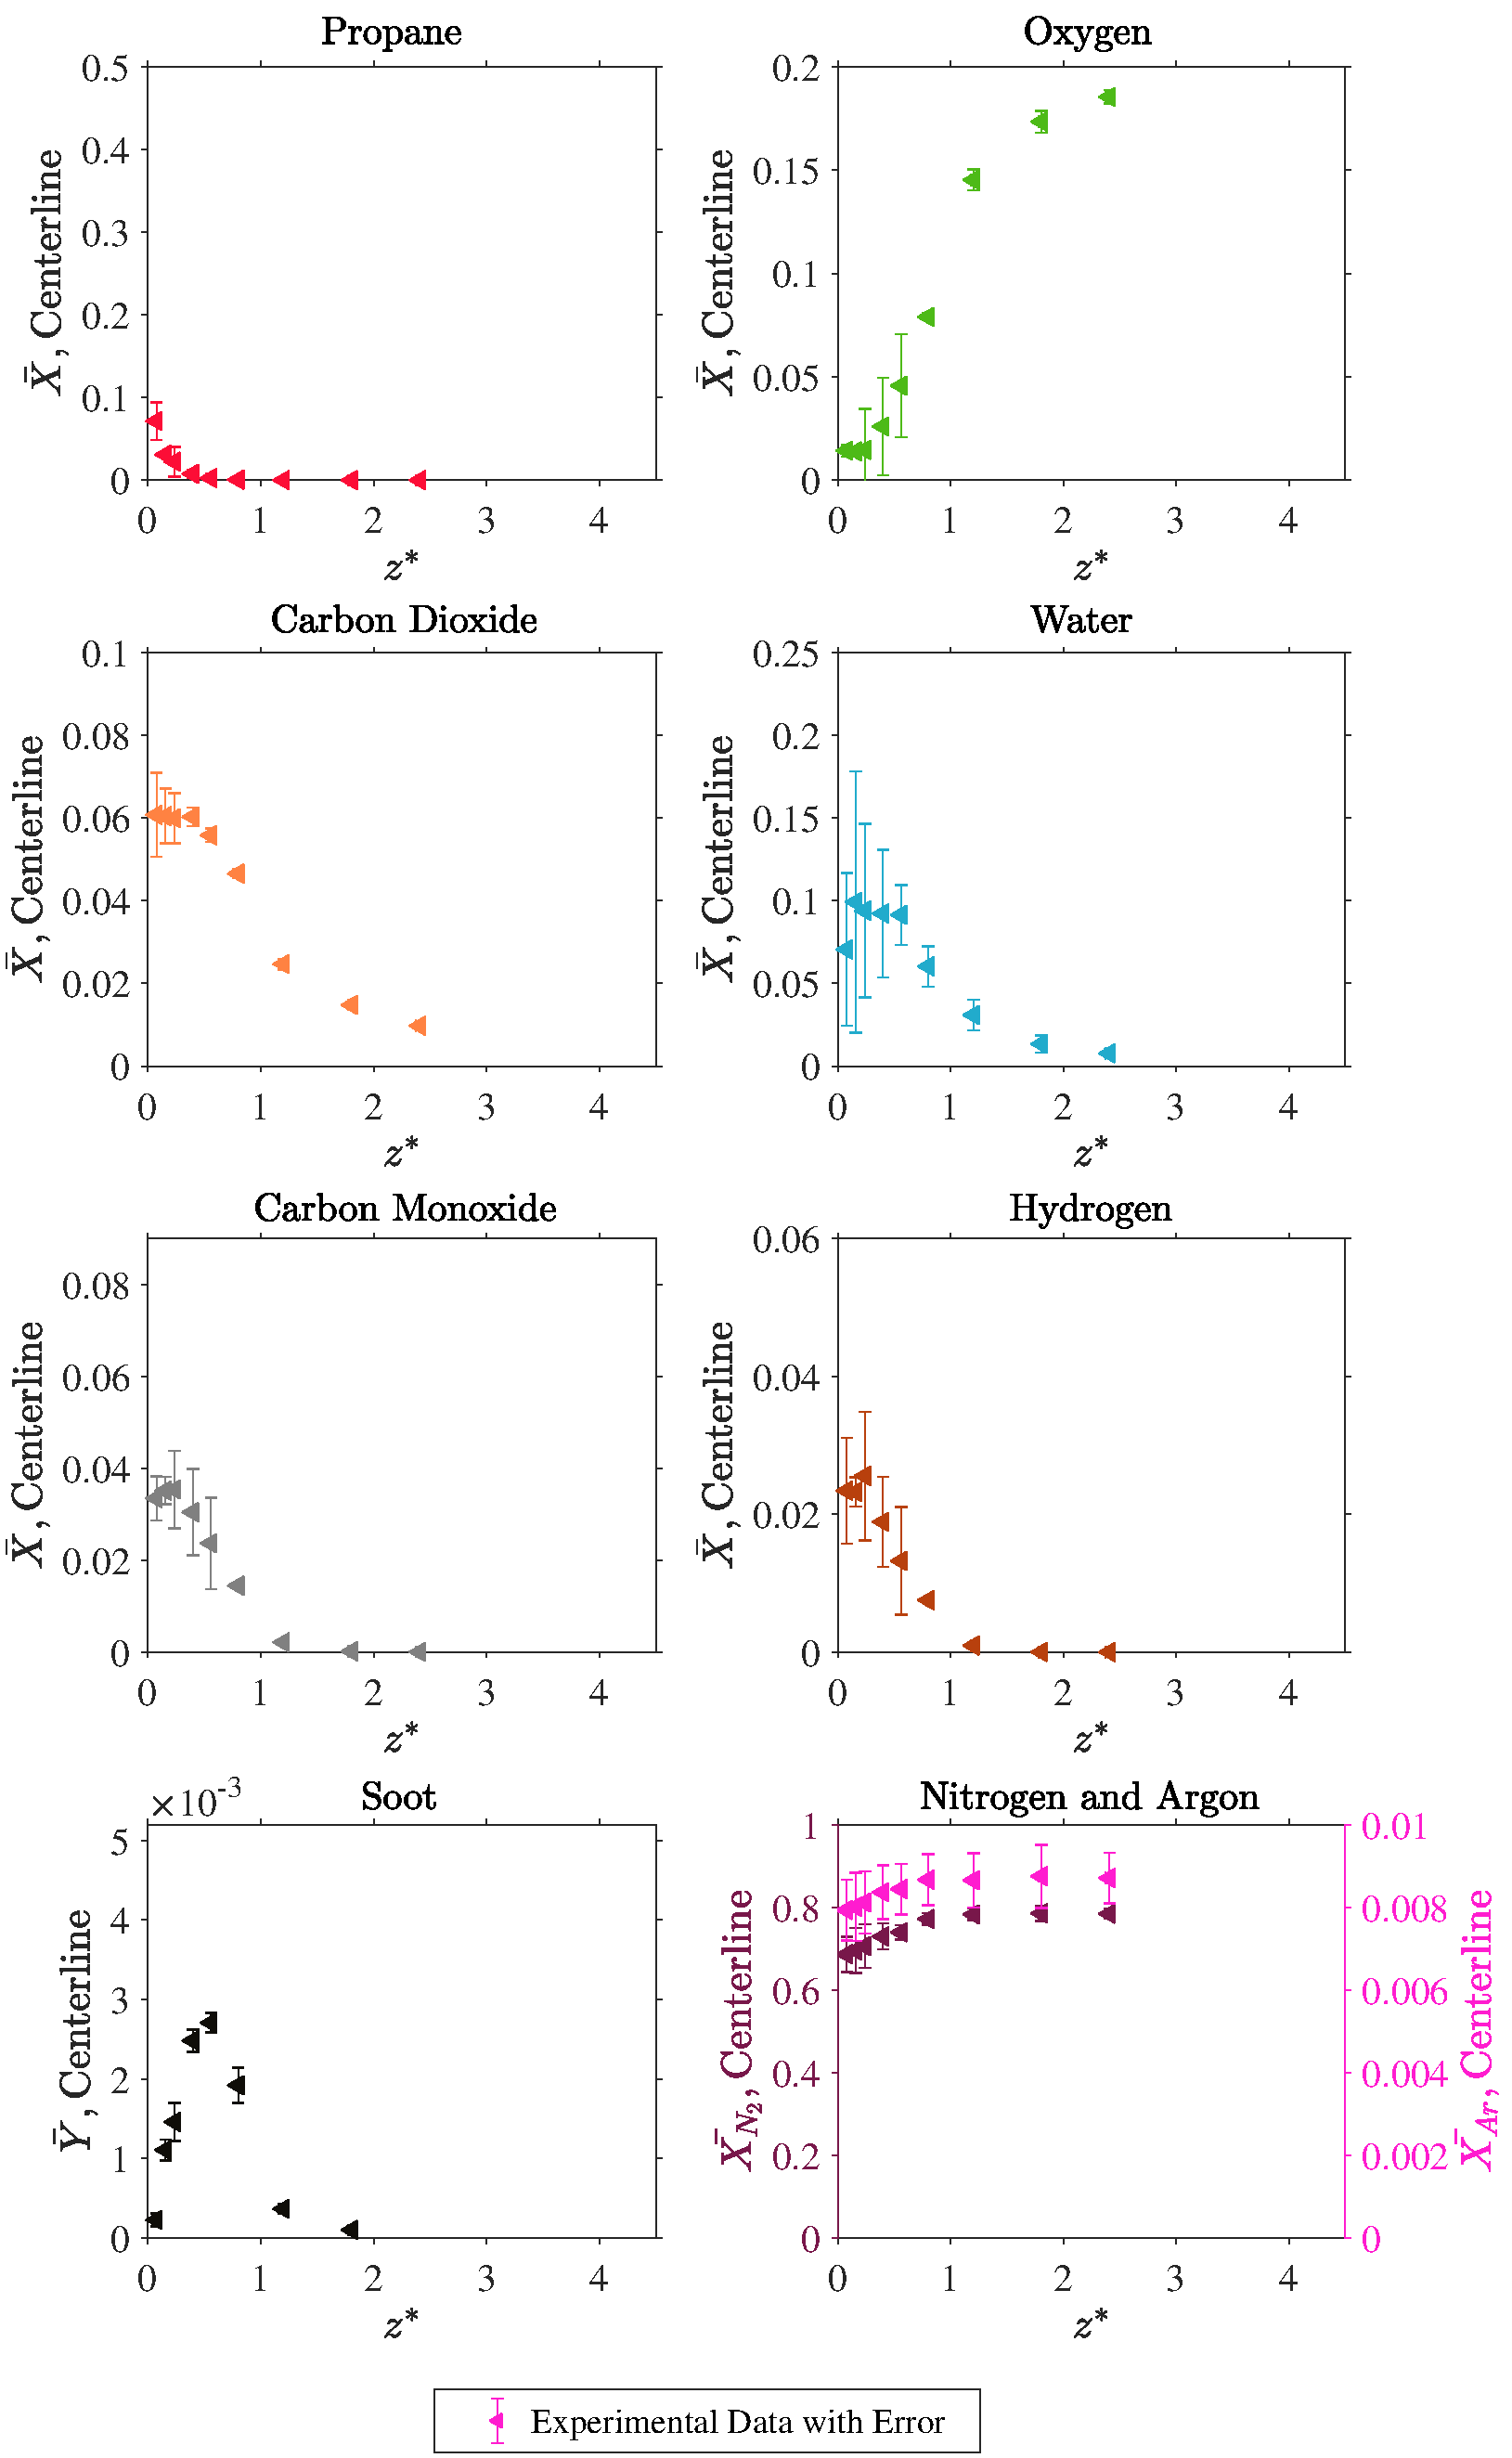
\includegraphics[width=10.75cm,keepaspectratio]{Propane 20KW_MOL_FRAC_Plot.pdf}
	\caption[Volume fractions of major species in the propane (20kW) plume]{Plot of volume fractions of all species identified in the propane (20~kW) pool fire as a function of $z^{*}$ along the pool centerline. The error is a combined uncertainty, further described in Section~\ref{sec:UncertaintyGasSpecies}.}
	\label{fig:Propane20kW_VOL_Frac_Major}
\end{figure}

\begin{figure}[!h]
	\centering
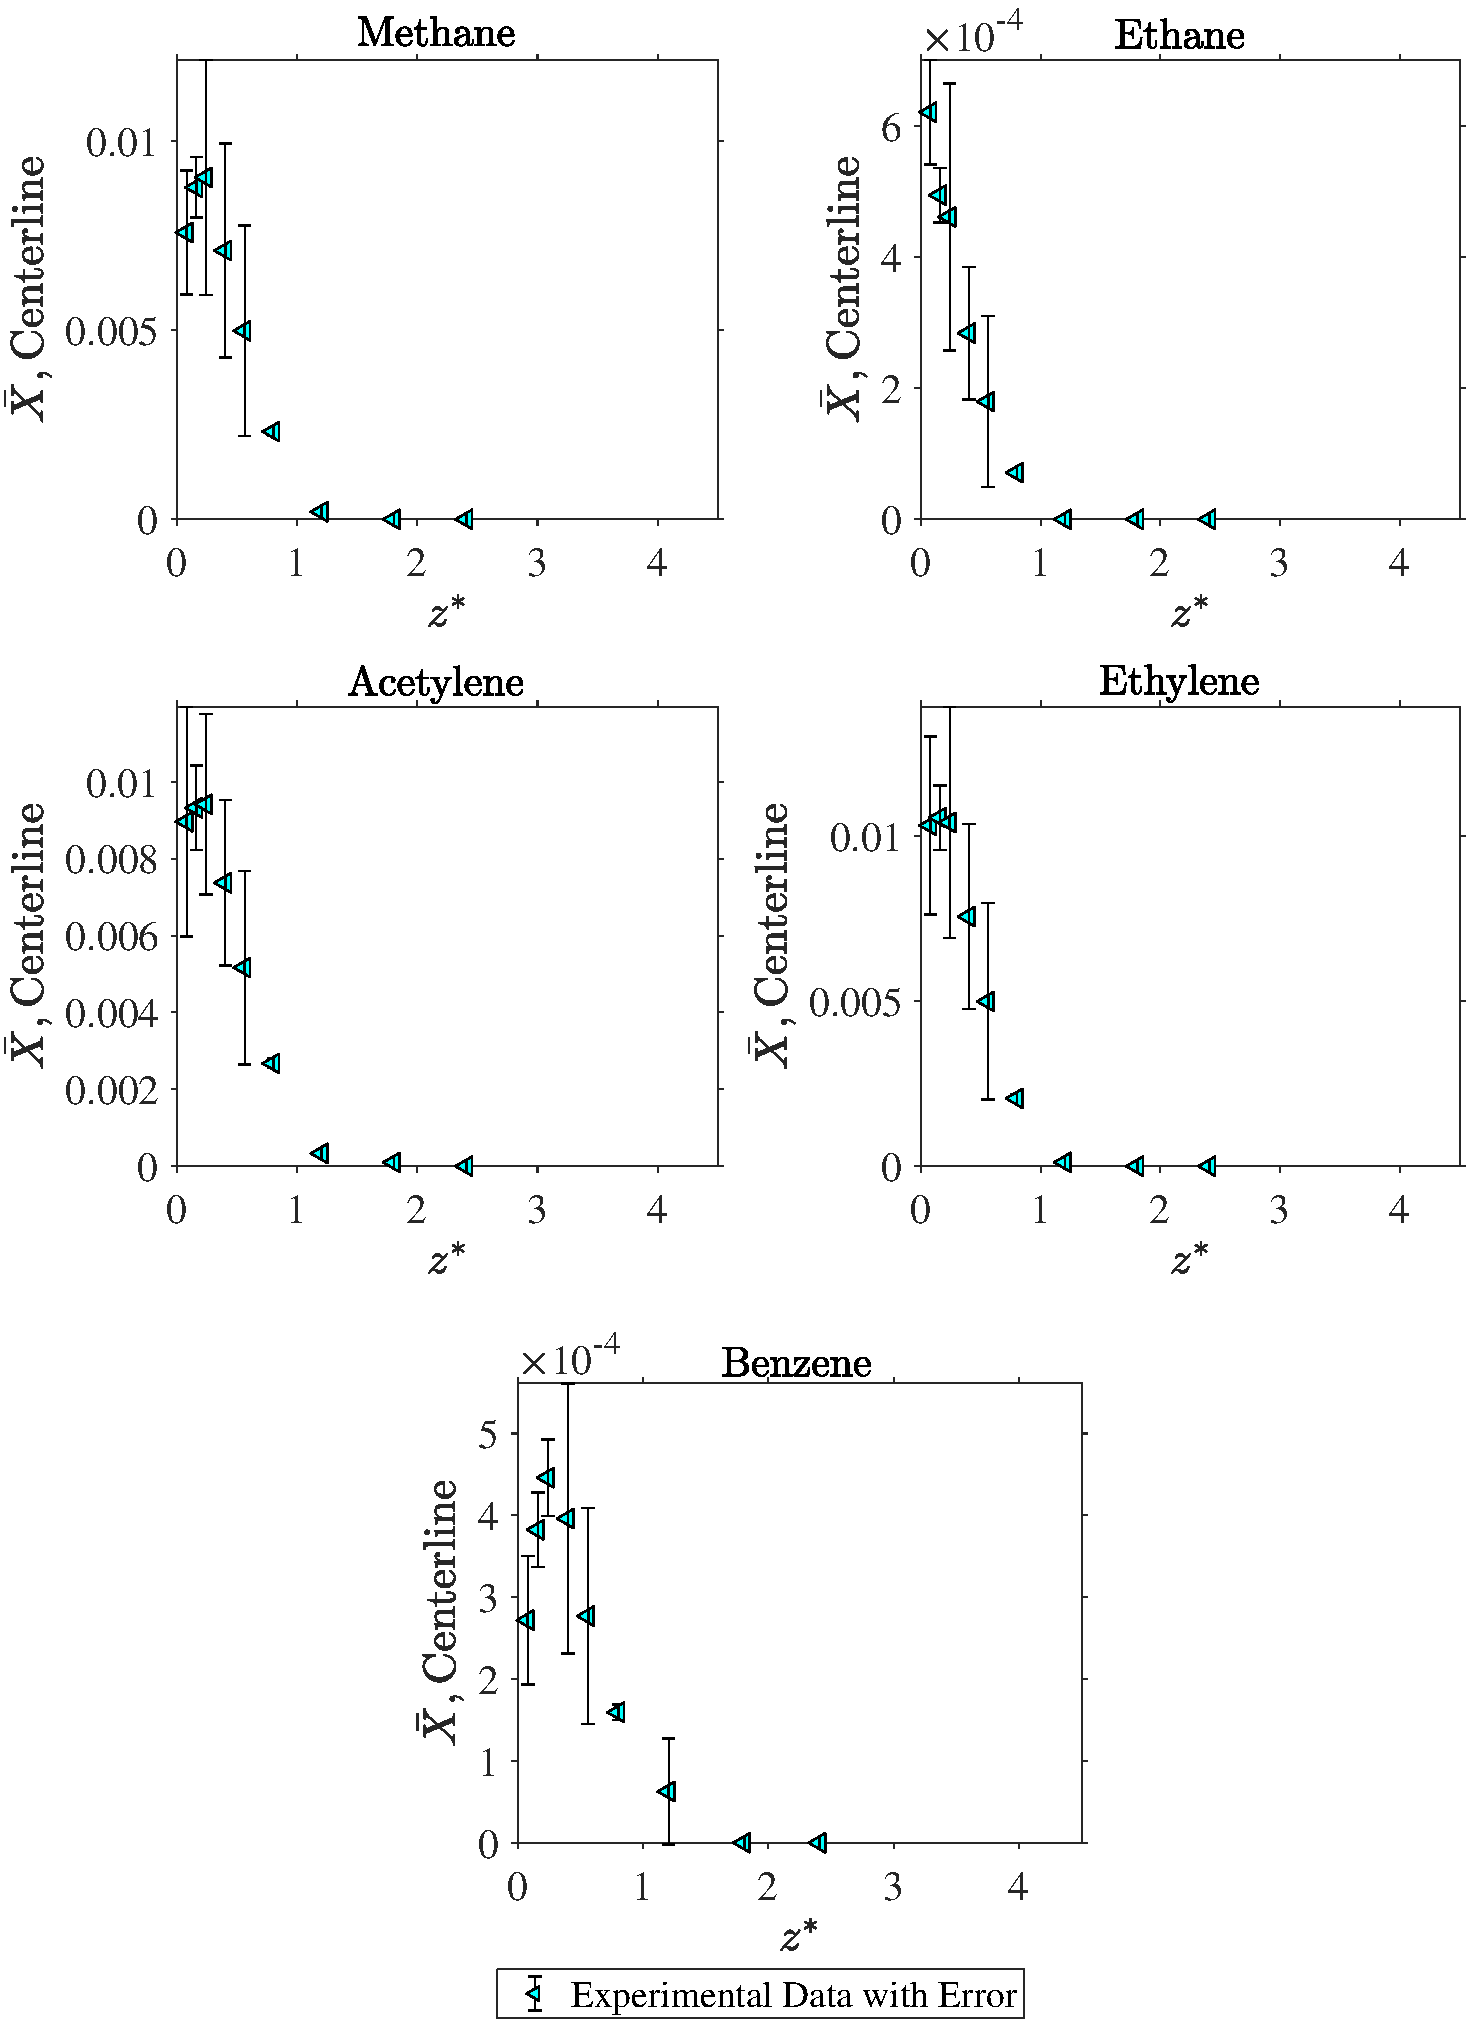
\includegraphics[width=10.75cm,keepaspectratio]{Propane 20KW_Inter_MOL_FRAC_Plot.pdf}
	\caption[Volume fractions of minor and trace species in the propane (20kW) plume]{Plot of volume fractions of minor and trace species identified in the propane (20~kW) pool fire as a function of $z^{*}$ along the pool centerline. The error presented here is a combined uncertainty, further described in Section~\ref{sec:UncertaintyGasSpecies}.}
	\label{fig:Propane20kW_VOL_Frac_Inter}
\end{figure}
\clearpage

\pagebreak
\subsection{Propane (34 kW)}
\label{ssec:Propane34kW_ALL_Vol_Frac}
\begin{figure}[!h]
	\centering
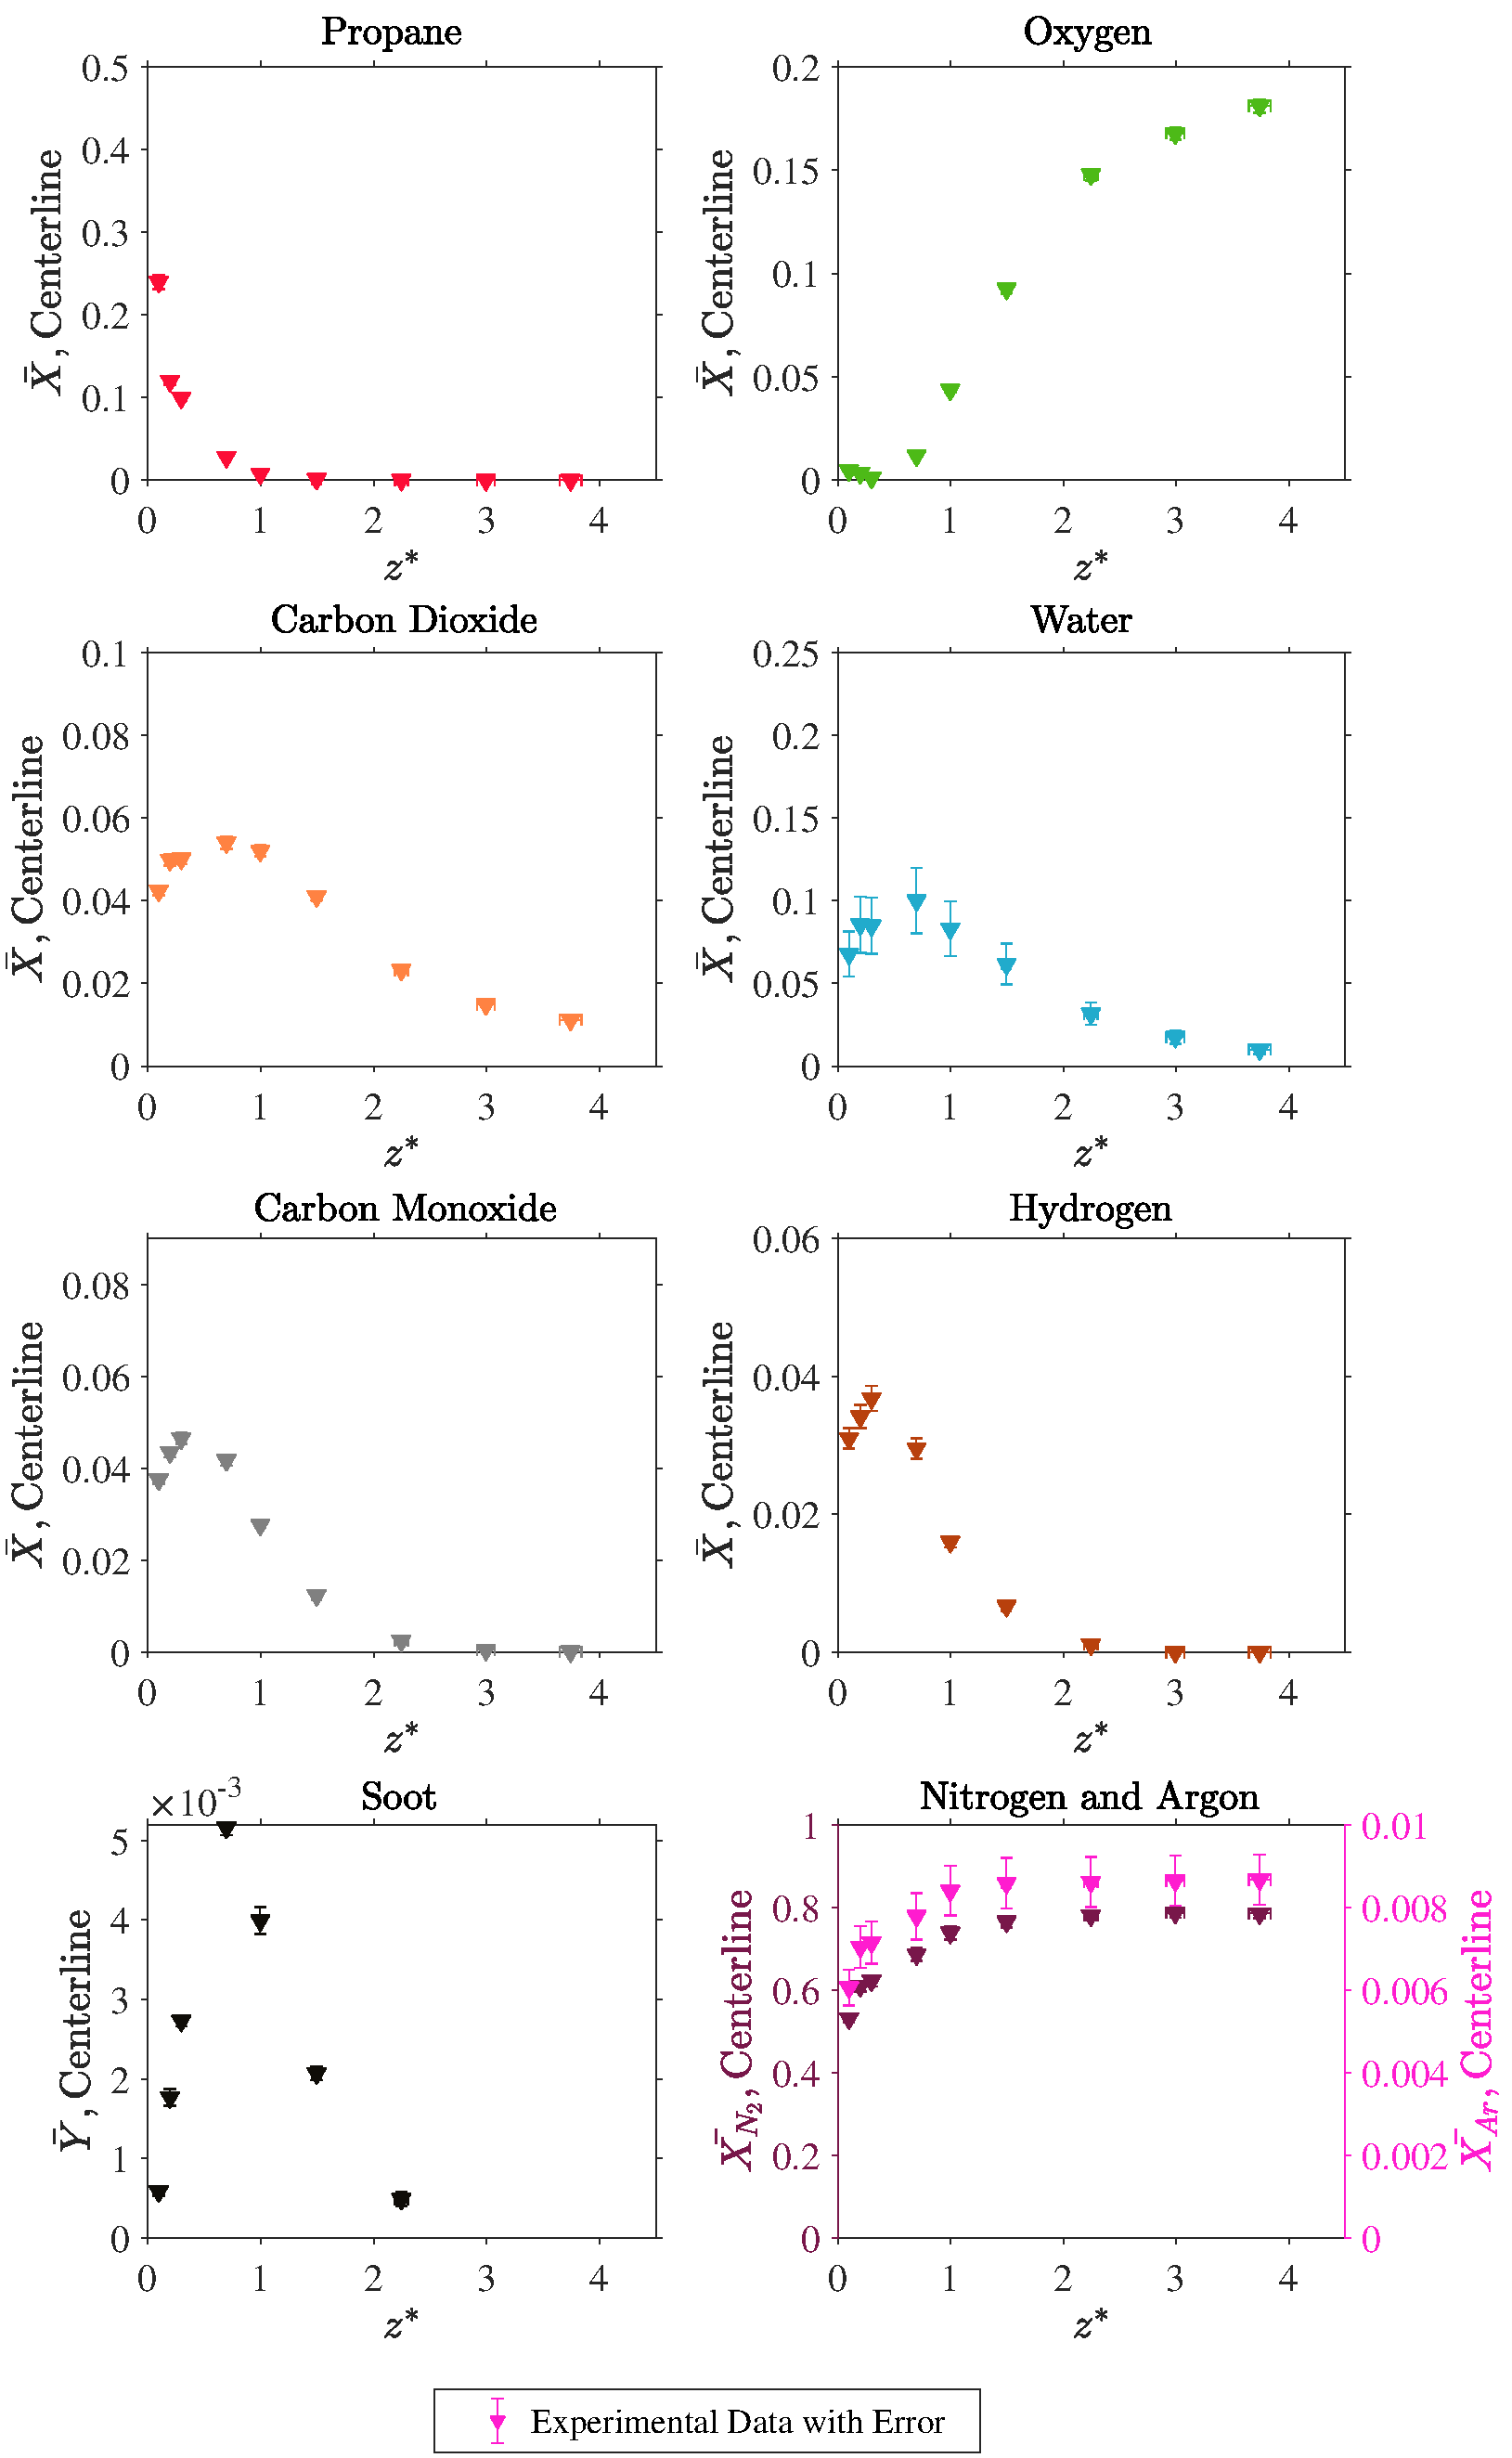
\includegraphics[width=10.75cm,keepaspectratio]{Propane 34KW_MOL_FRAC_Plot.pdf}
	\caption[Volume fractions of major species in the propane (34 kW) plume]{Plot of volume fractions of all species identified in the propane (34~kW) pool fire as a function of $z^{*}$ along the pool centerline. The error is a combined uncertainty, further described in Section~\ref{sec:UncertaintyGasSpecies}.}
	\label{fig:Propane20kW_VOL_Frac_Major}
\end{figure}

\begin{figure}[!h]
	\centering
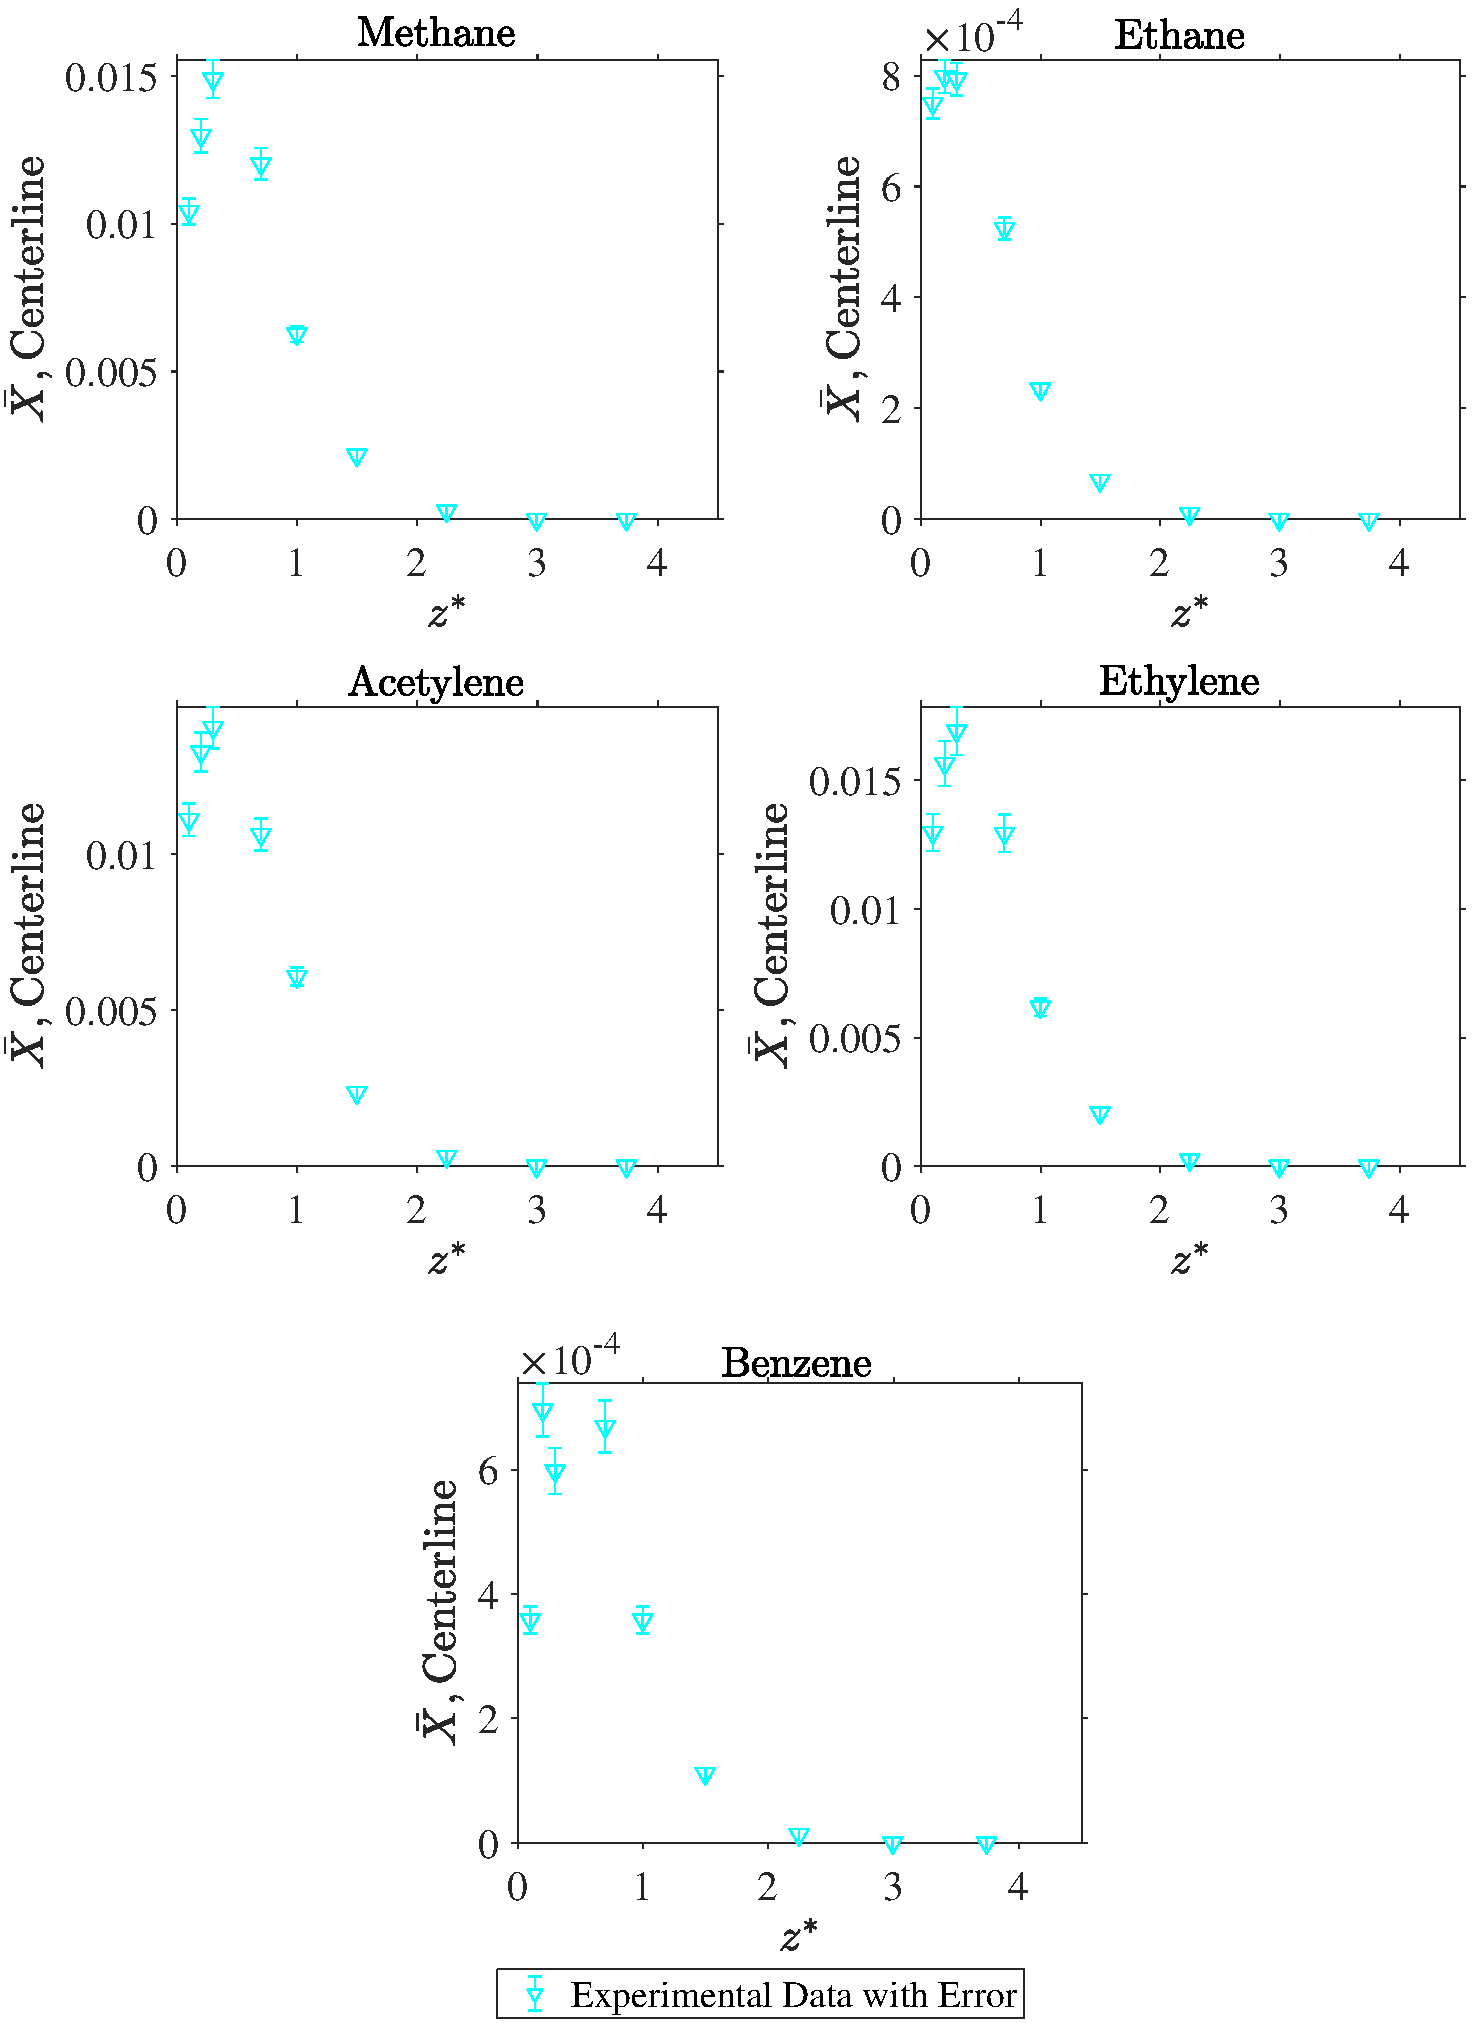
\includegraphics[width=10.75cm,keepaspectratio]{Propane 34KW_Inter_MOL_FRAC_Plot.pdf}
	\caption[Volume fractions of minor and trace species in the propane (34 kW) plume]{Plot of volume fractions of minor and trace species identified in the propane (34~kW) pool fire as a function of $z^{*}$ along the pool centerline. The error presented here is a combined uncertainty, further described in Section~\ref{sec:UncertaintyGasSpecies}.}
	\label{fig:Propane20kW_VOL_Frac_Inter}
\end{figure}
\clearpage

\section{Figures of Averaged Mass Fractions}\label{sec:Mix_Frac_Figs}

\subsection{Methanol}
\label{ssec:Methanol_ALL_Mix_Frac}

\begin{figure}[!h]
	\centering
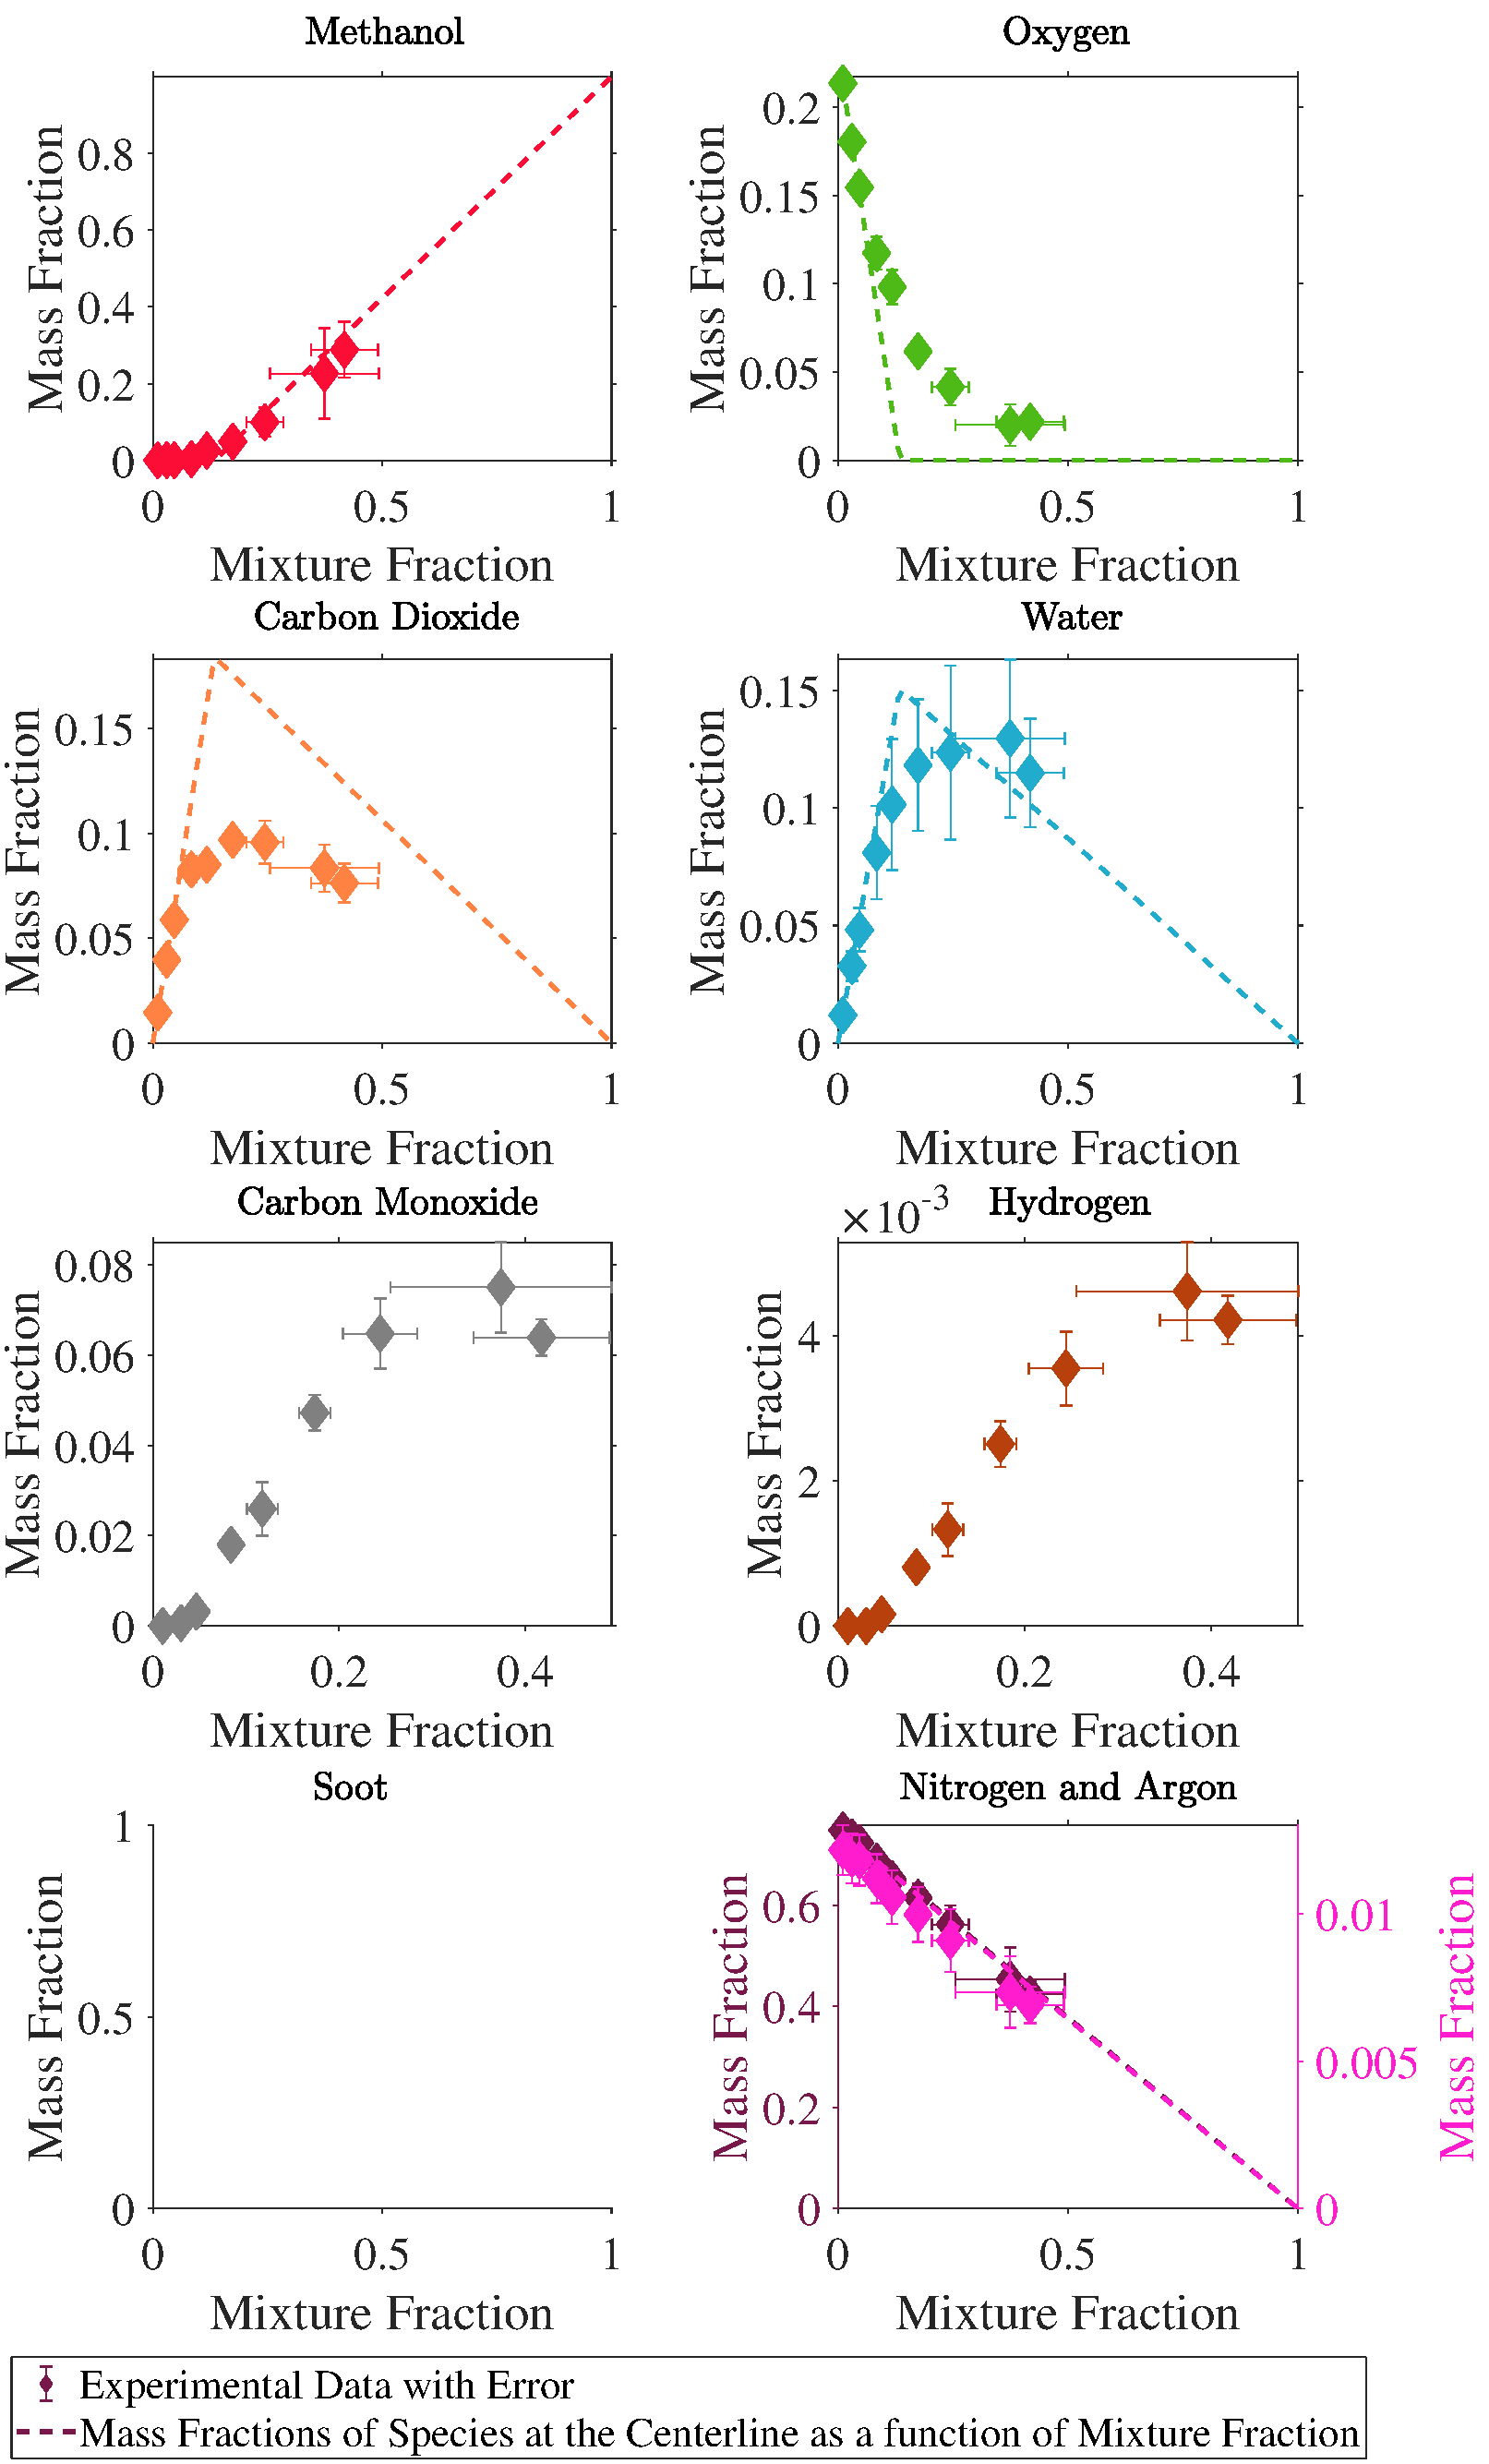
\includegraphics[width=10.25cm,keepaspectratio]{Methanol_Mixture_Fraction_Major_Plot.pdf}
	\caption[Species mass fractions superimposed on methanol state relations]{Plot of mass fractions, with uncertainty, of major species identified in the methanol pool fire centerline as function of mixture fraction. The uncertainty is a combined uncertainty, discussed in further detail in Sections~\ref{sec:Uncertainty_Ver_Scheme} and \ref{sec:UncertaintyGasSpecies} for the mass fraction and mixture fractions, respectively.}
	\label{fig:Methanol_MIX_Frac_Major}
\end{figure}

\pagebreak

\subsection{Ethanol}
\label{ssec:Ethanol_ALL_Mix_Frac}
\begin{figure}[h!]
	\centering
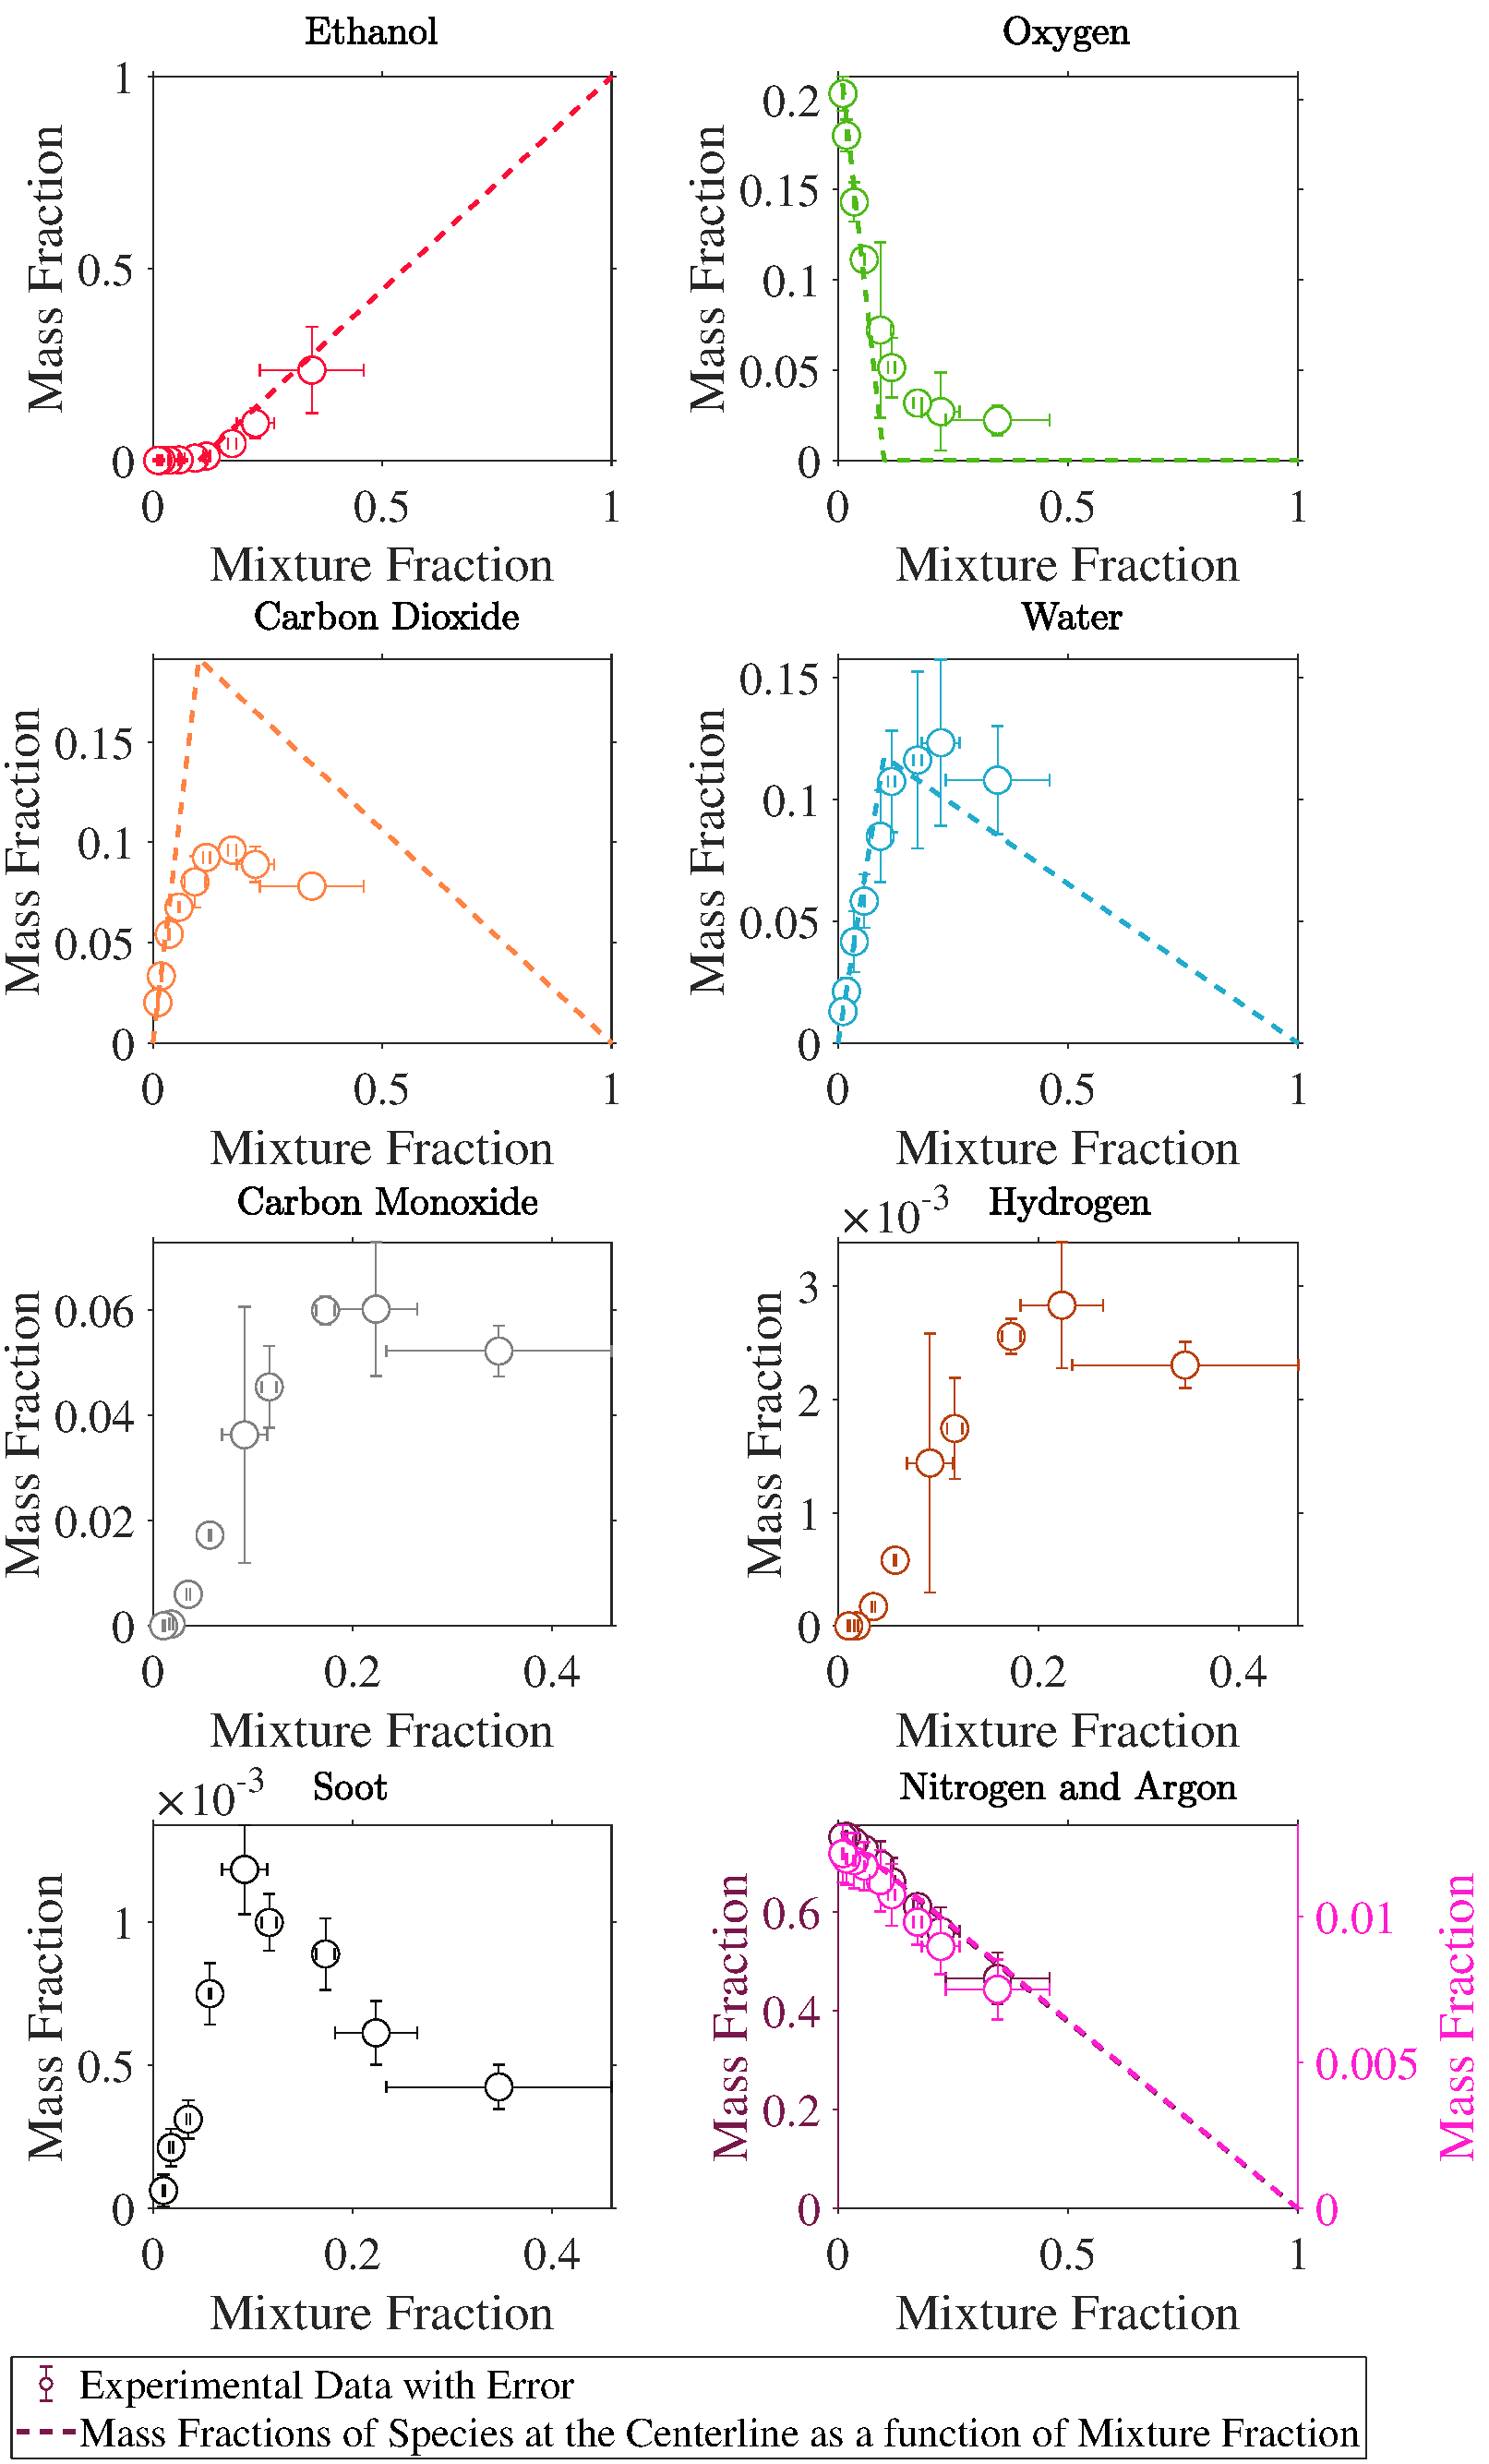
\includegraphics[width=10.5cm,keepaspectratio]{Ethanol_Mixture_Fraction_Major_Plot.pdf}
	\caption[Species mass fractions superimposed on ethanol state relations]{Plot of mass fractions, with uncertainty, of major species identified in the ethanol pool fire centerline as function of mixture fraction. The uncertainty is a combined uncertainty, discussed in further detail in Sections~\ref{sec:Uncertainty_Ver_Scheme} and \ref{sec:UncertaintyGasSpecies} for the mass fraction and mixture fractions, respectively.}
	\label{fig:Ethanol_MIX_Frac_Major}
\end{figure}

\pagebreak

\subsection{Acetone}
\label{ssec:Acetone_ALL_Mix_Frac}
\begin{figure}[!h]
	\centering
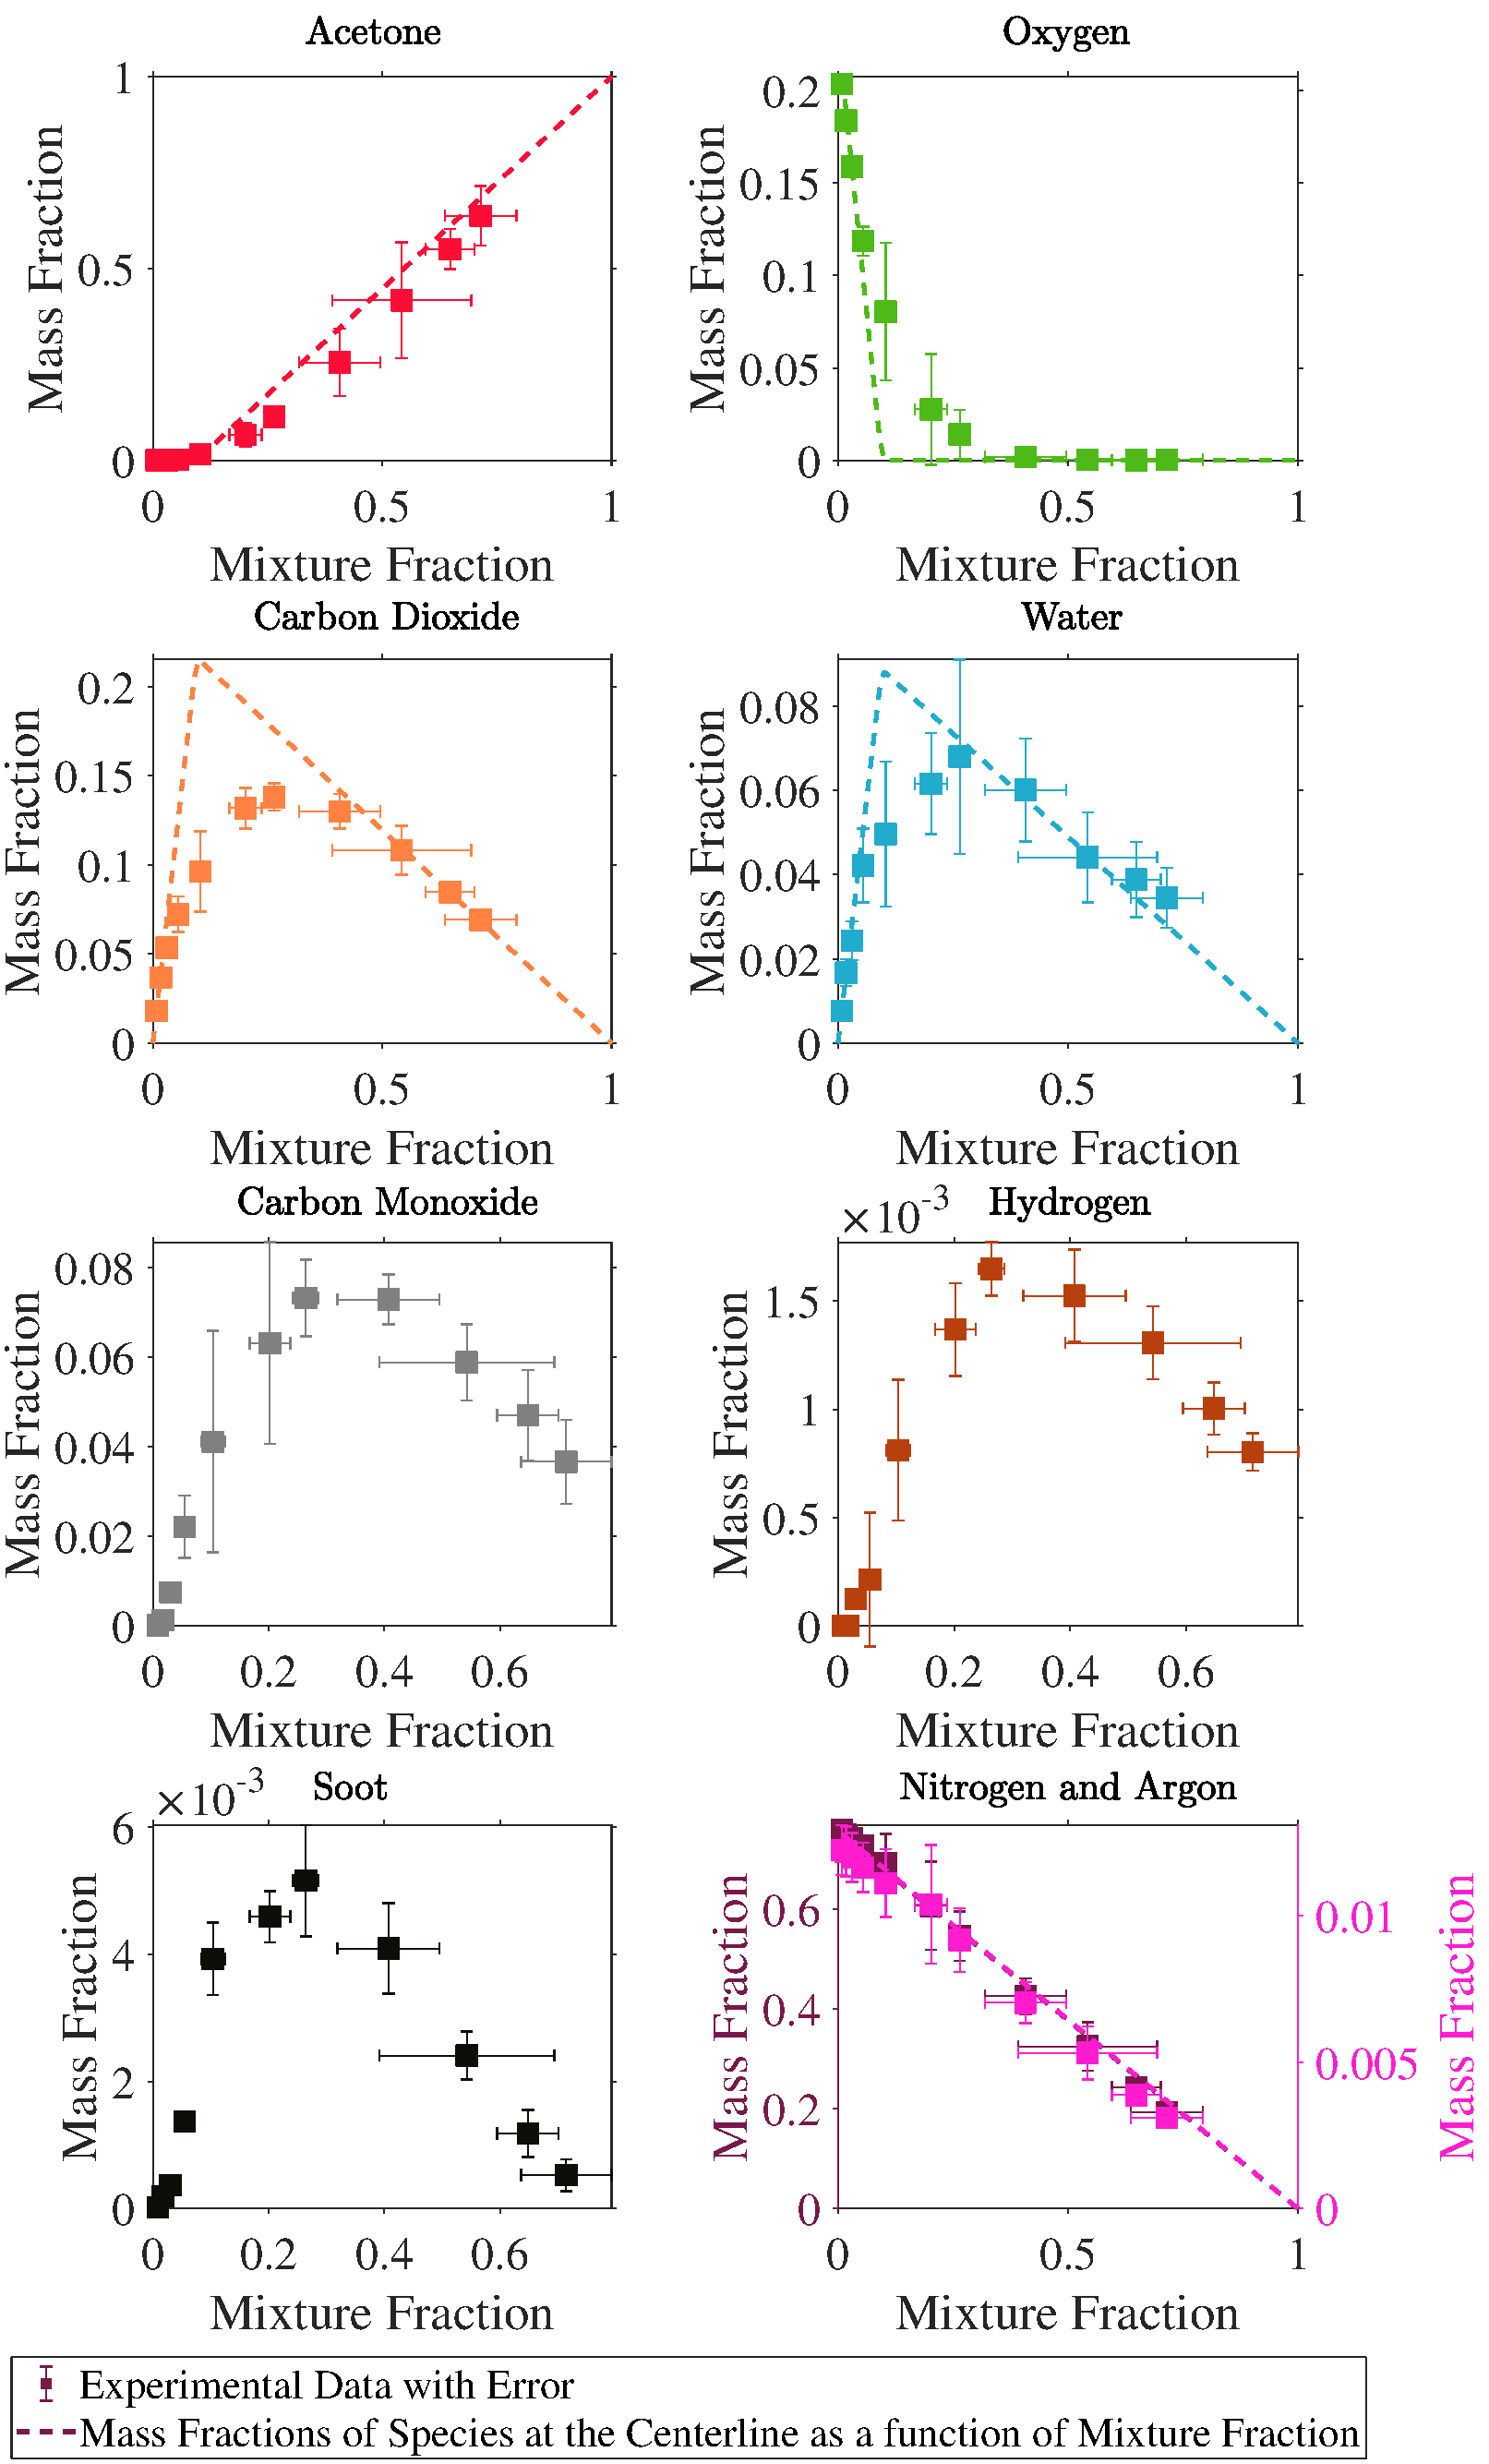
\includegraphics[width=10.5cm,keepaspectratio]{Acetone_Mixture_Fraction_Major_Plot.pdf}
	\caption[Species mass fractions superimposed on acetone state relations]{Plot of mass fractions, with uncertainty, of major species identified in the acetone pool fire centerline as function of mixture fraction. The uncertainty is a combined uncertainty, discussed in further detail in Sections~\ref{sec:Uncertainty_Ver_Scheme} and \ref{sec:UncertaintyGasSpecies} for the mass fraction and mixture fractions, respectively.}
	\label{fig:Acetone_MIX_Frac_Major}
\end{figure}

\pagebreak

\subsection{Methane}
\label{ssec:Methane_ALL_Mix_Frac}
\begin{figure}[!h]
	\centering
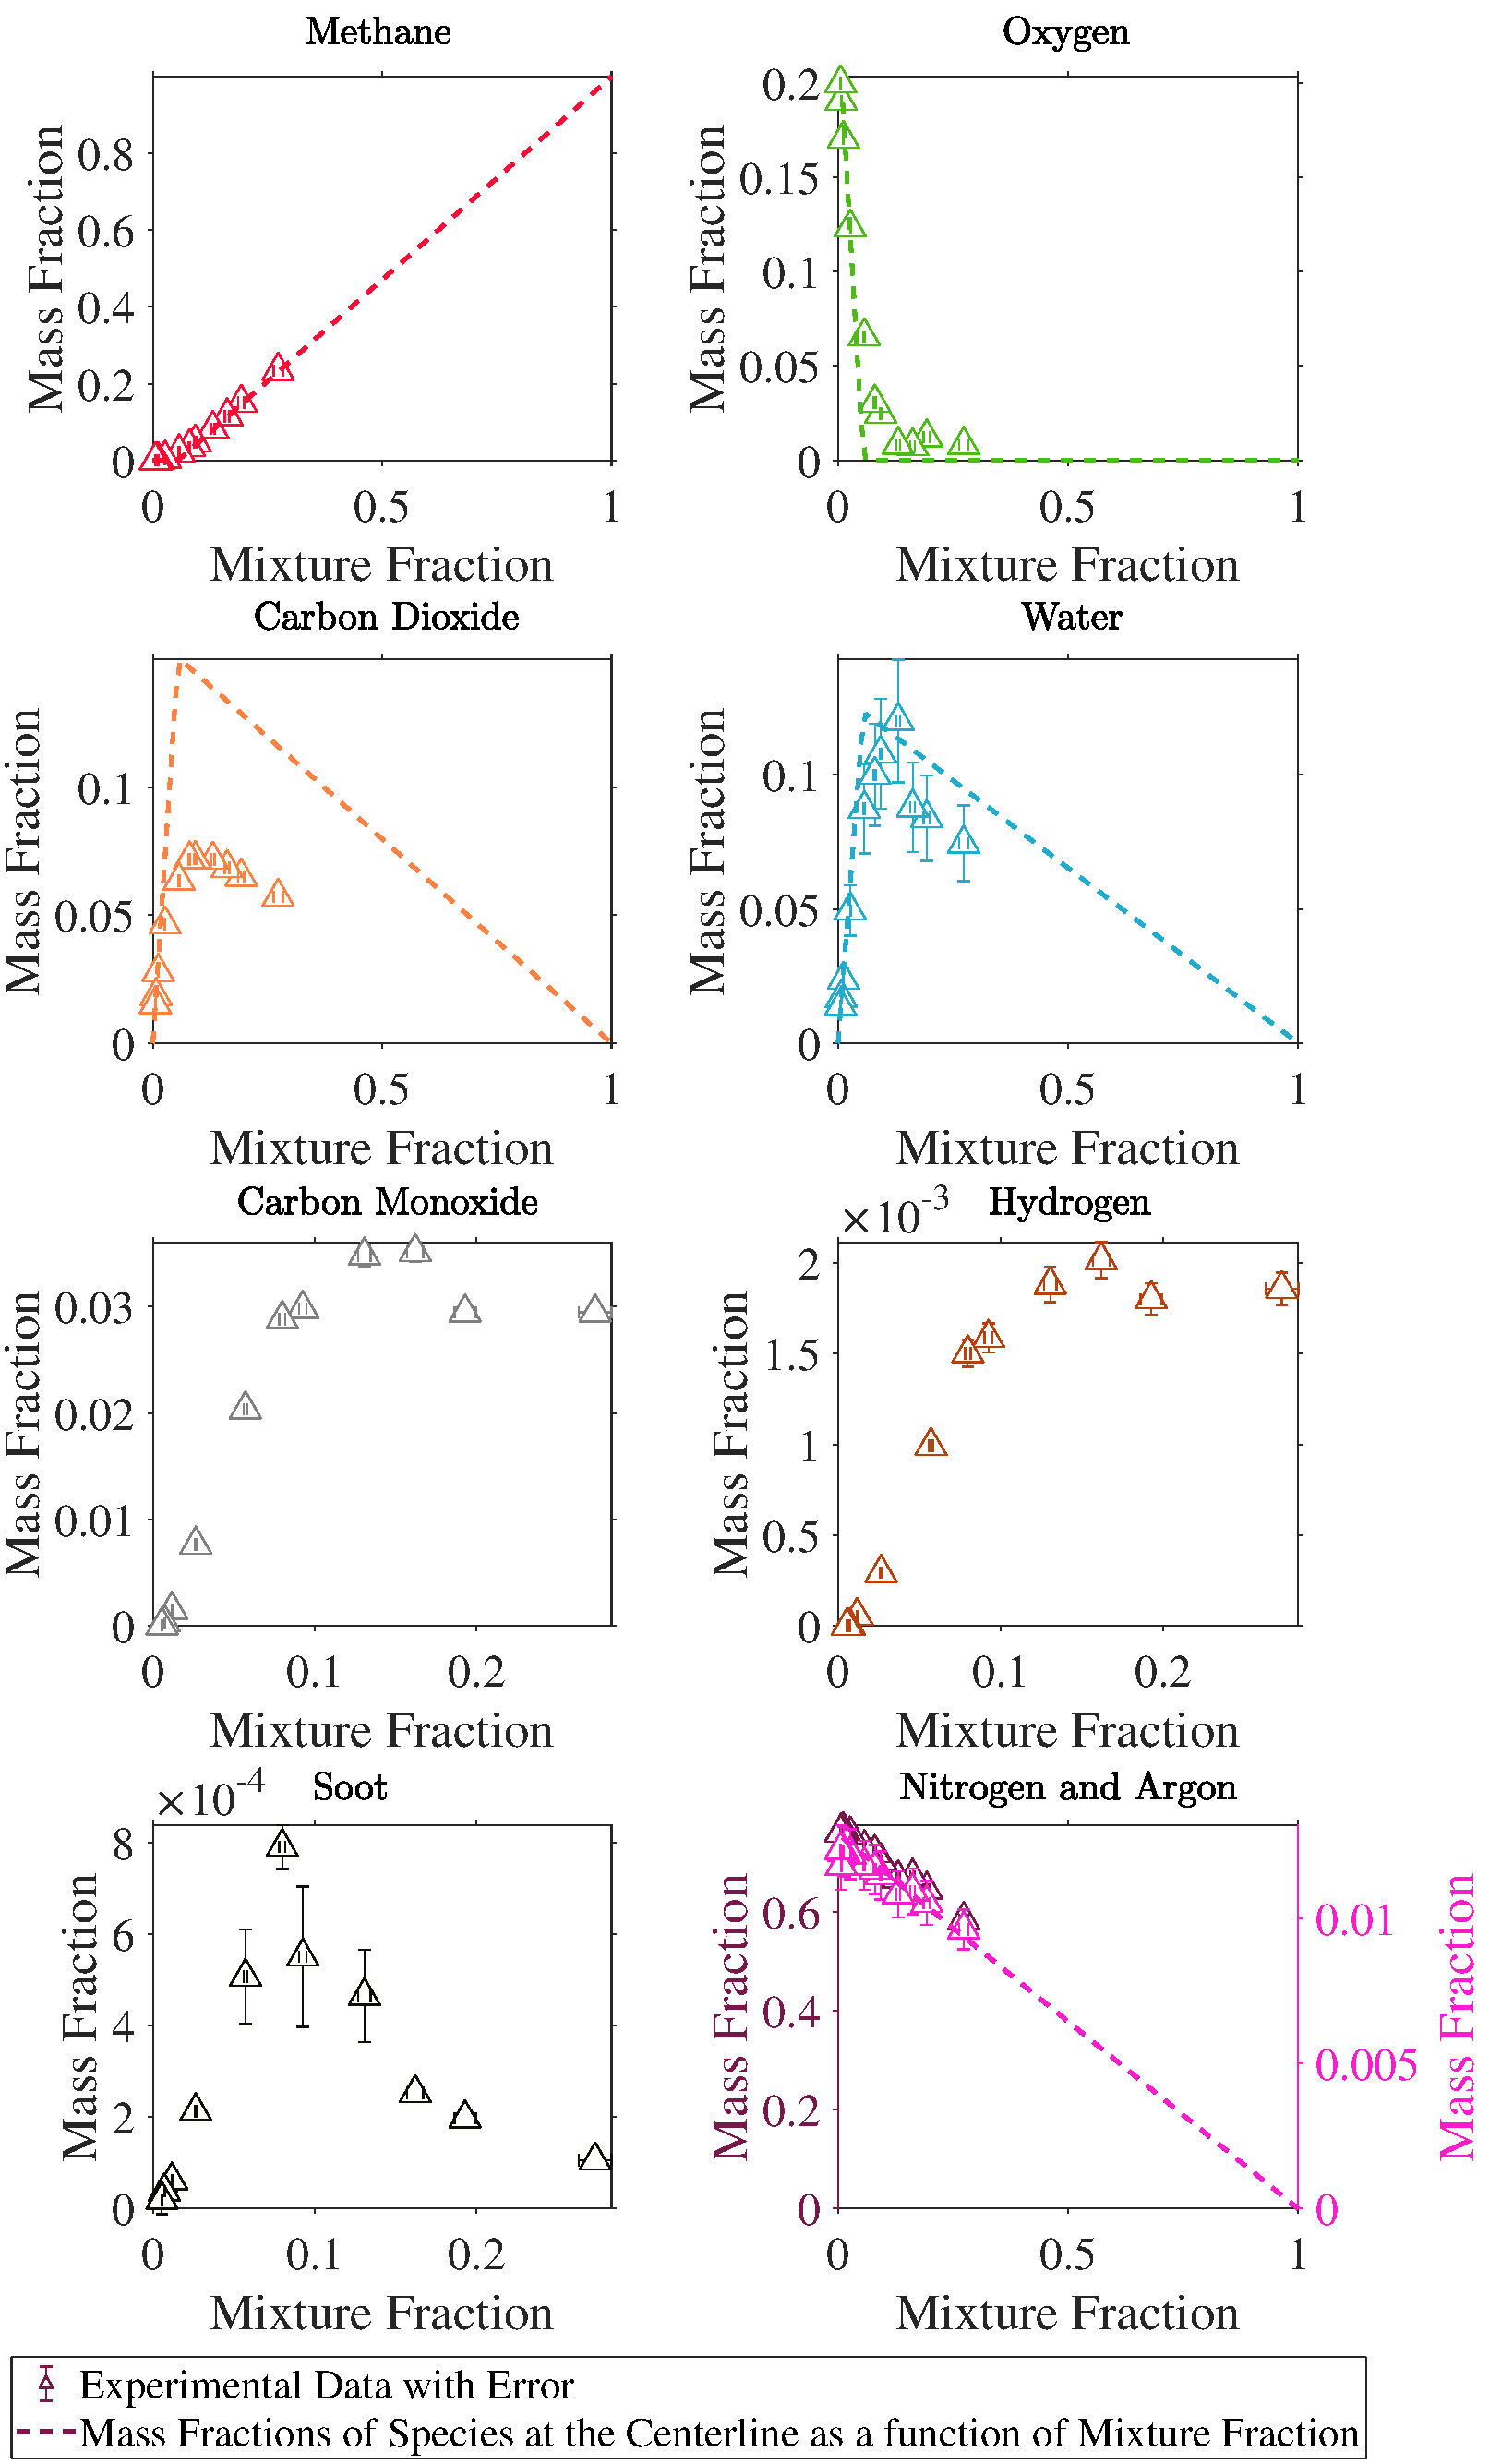
\includegraphics[width=10.5cm,keepaspectratio]{Methane_Mixture_Fraction_Major_Plot.pdf}
	\caption[Species mass fractions superimposed on methane state relations]{Plot of mass fractions, with uncertainty, of major species identified in the methane pool fire centerline as function of mixture fraction. The uncertainty is a combined uncertainty, discussed in further detail in Sections~\ref{sec:Uncertainty_Ver_Scheme} and \ref{sec:UncertaintyGasSpecies} for the mass fraction and mixture fractions, respectively.}
	\label{fig:Methane_MIX_Frac_Major}
\end{figure}

\pagebreak

\subsection{Propane (20 kW)}
\label{ssec:Propane20KW_ALL_Mix_Frac}
\begin{figure}[!h]
	\centering
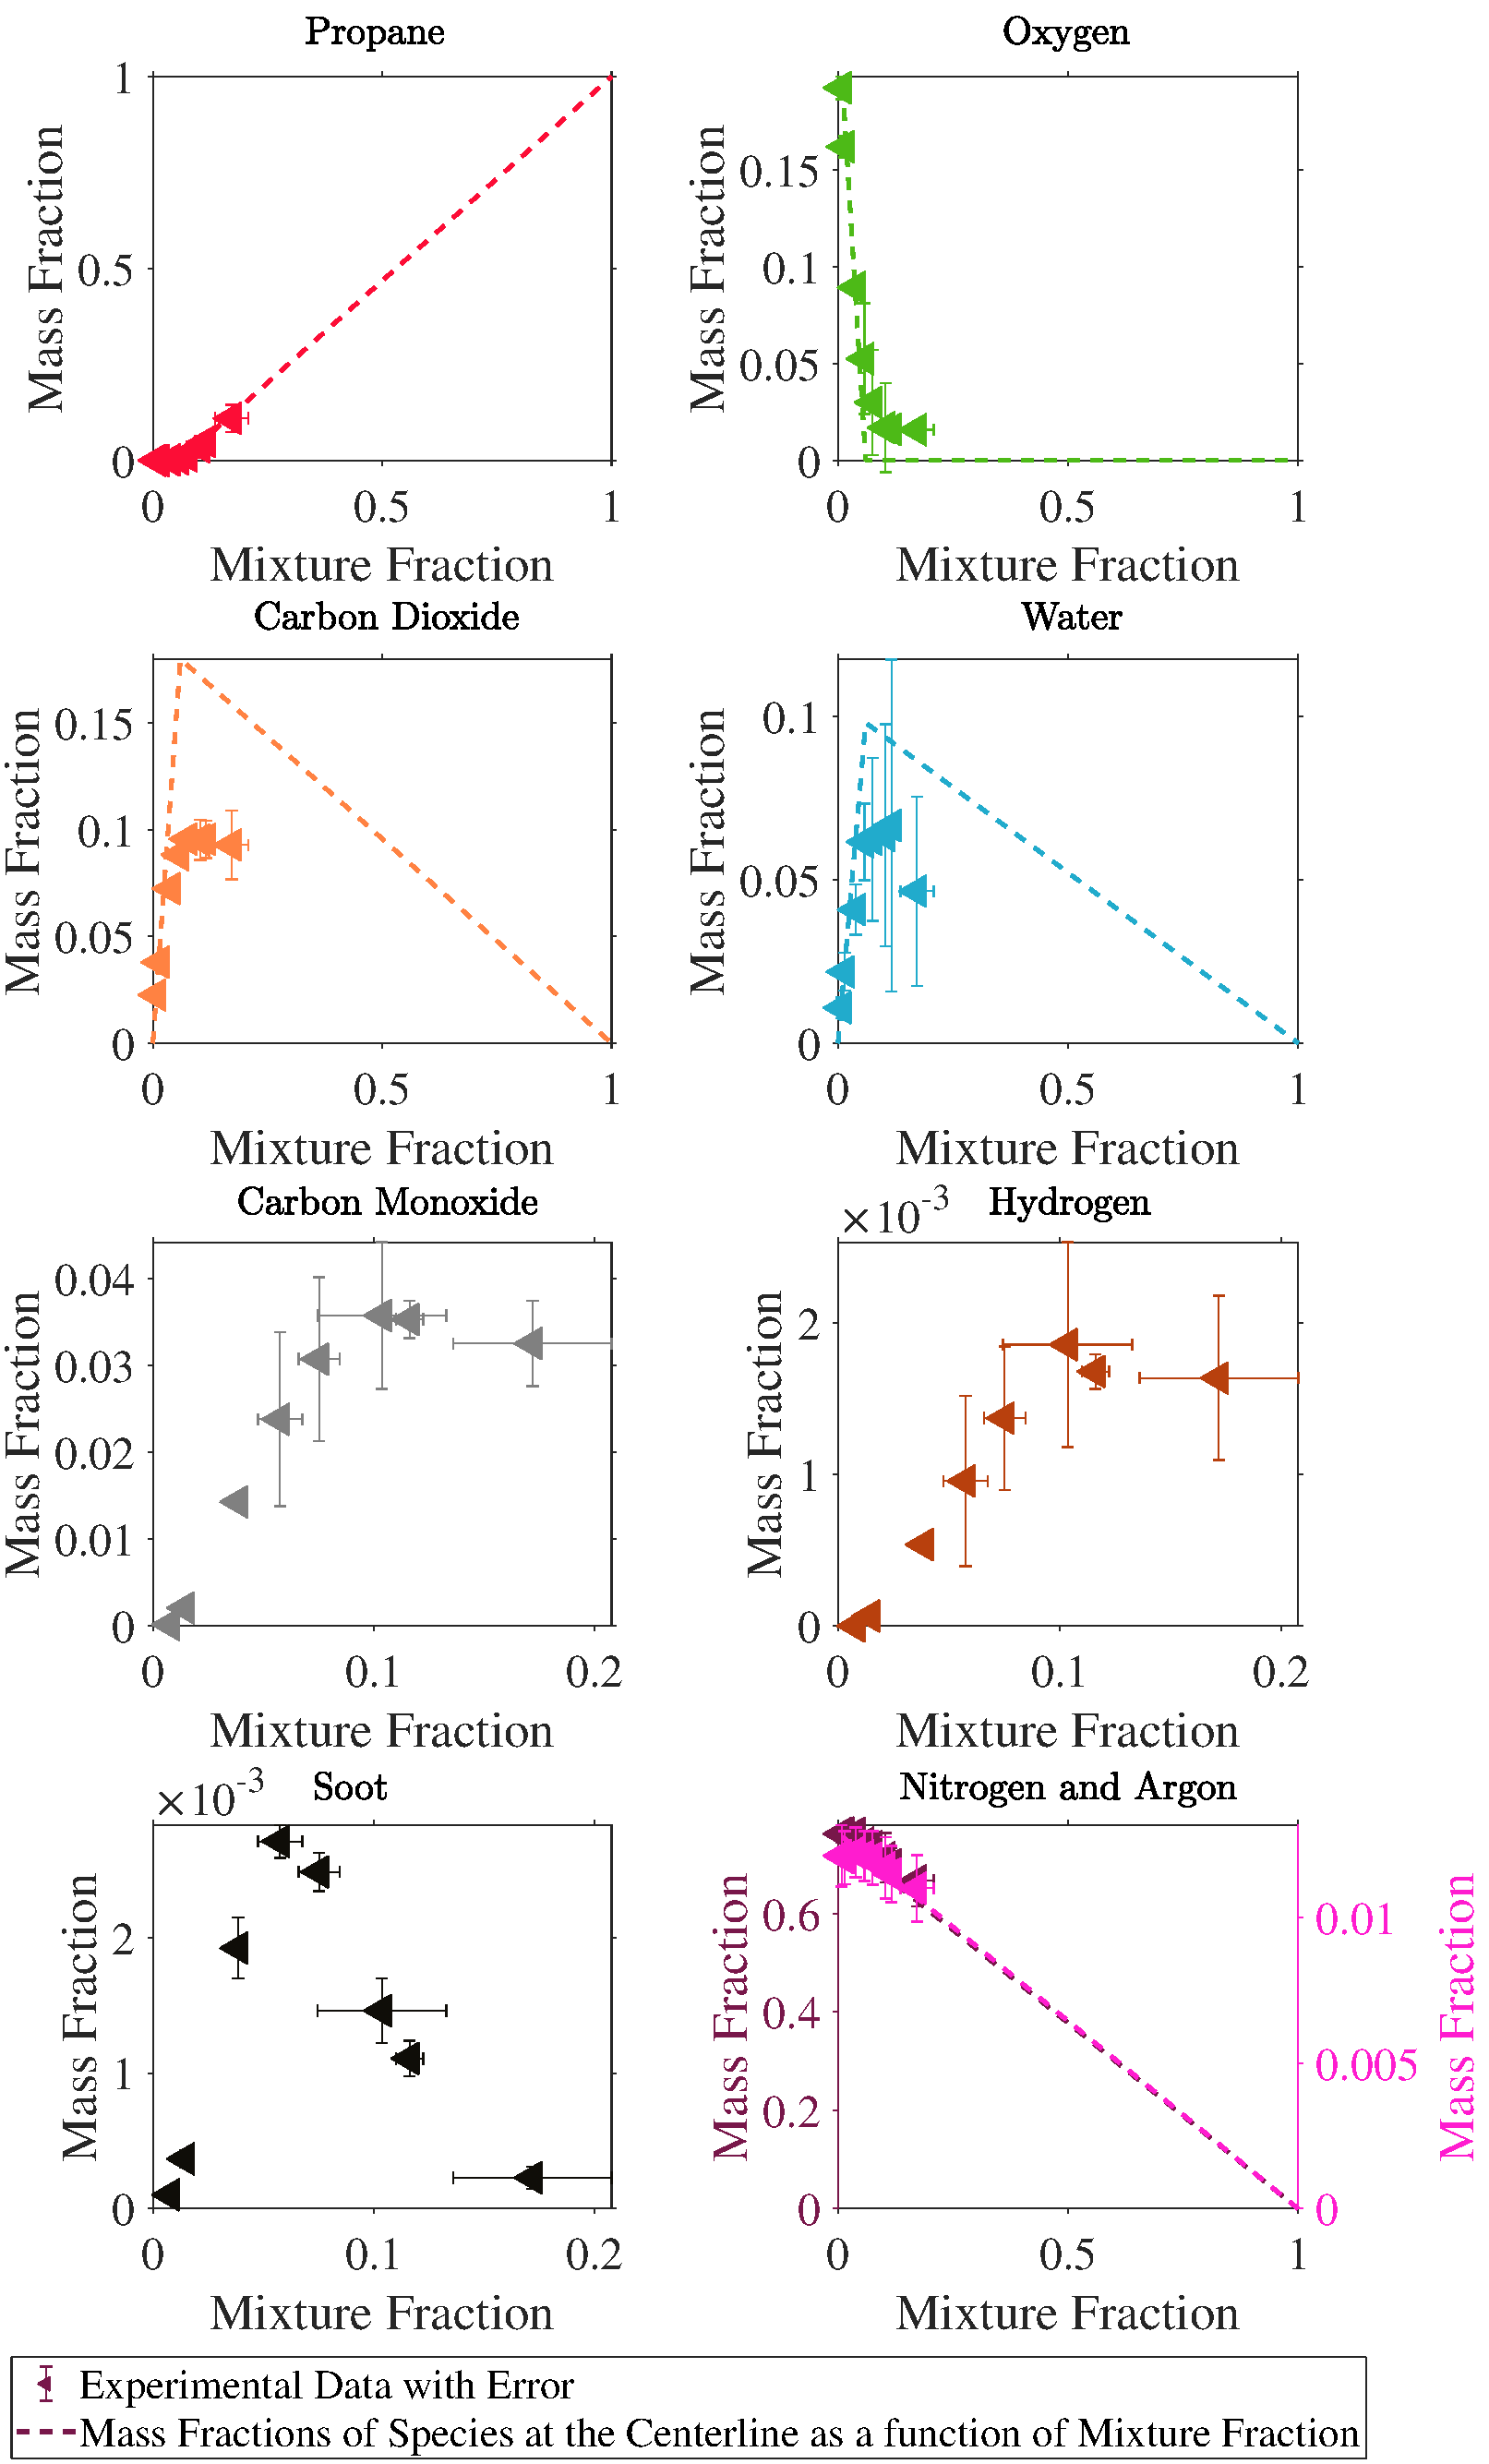
\includegraphics[width=10.5cm,keepaspectratio]{Propane 20KW_Mixture_Fraction_Major_Plot.pdf}
	\caption[Species mass fractions superimposed on propane (20 kW) state relations]{Plot of mass fractions, with uncertainty, of major species identified in the propane (20 kW) pool fire centerline as function of mixture fraction. The uncertainty is a combined uncertainty, discussed in further detail in Sections~\ref{sec:Uncertainty_Ver_Scheme} and \ref{sec:UncertaintyGasSpecies} for the mass fraction and mixture fractions, respectively.}
	\label{fig:Propane20KW_MIX_Frac_Major}
\end{figure}

\pagebreak

\subsection{Propane (34 kW)}
\label{ssec:Propane34KW_ALL_Mix_Frac}
\begin{figure}[!h]
	\centering
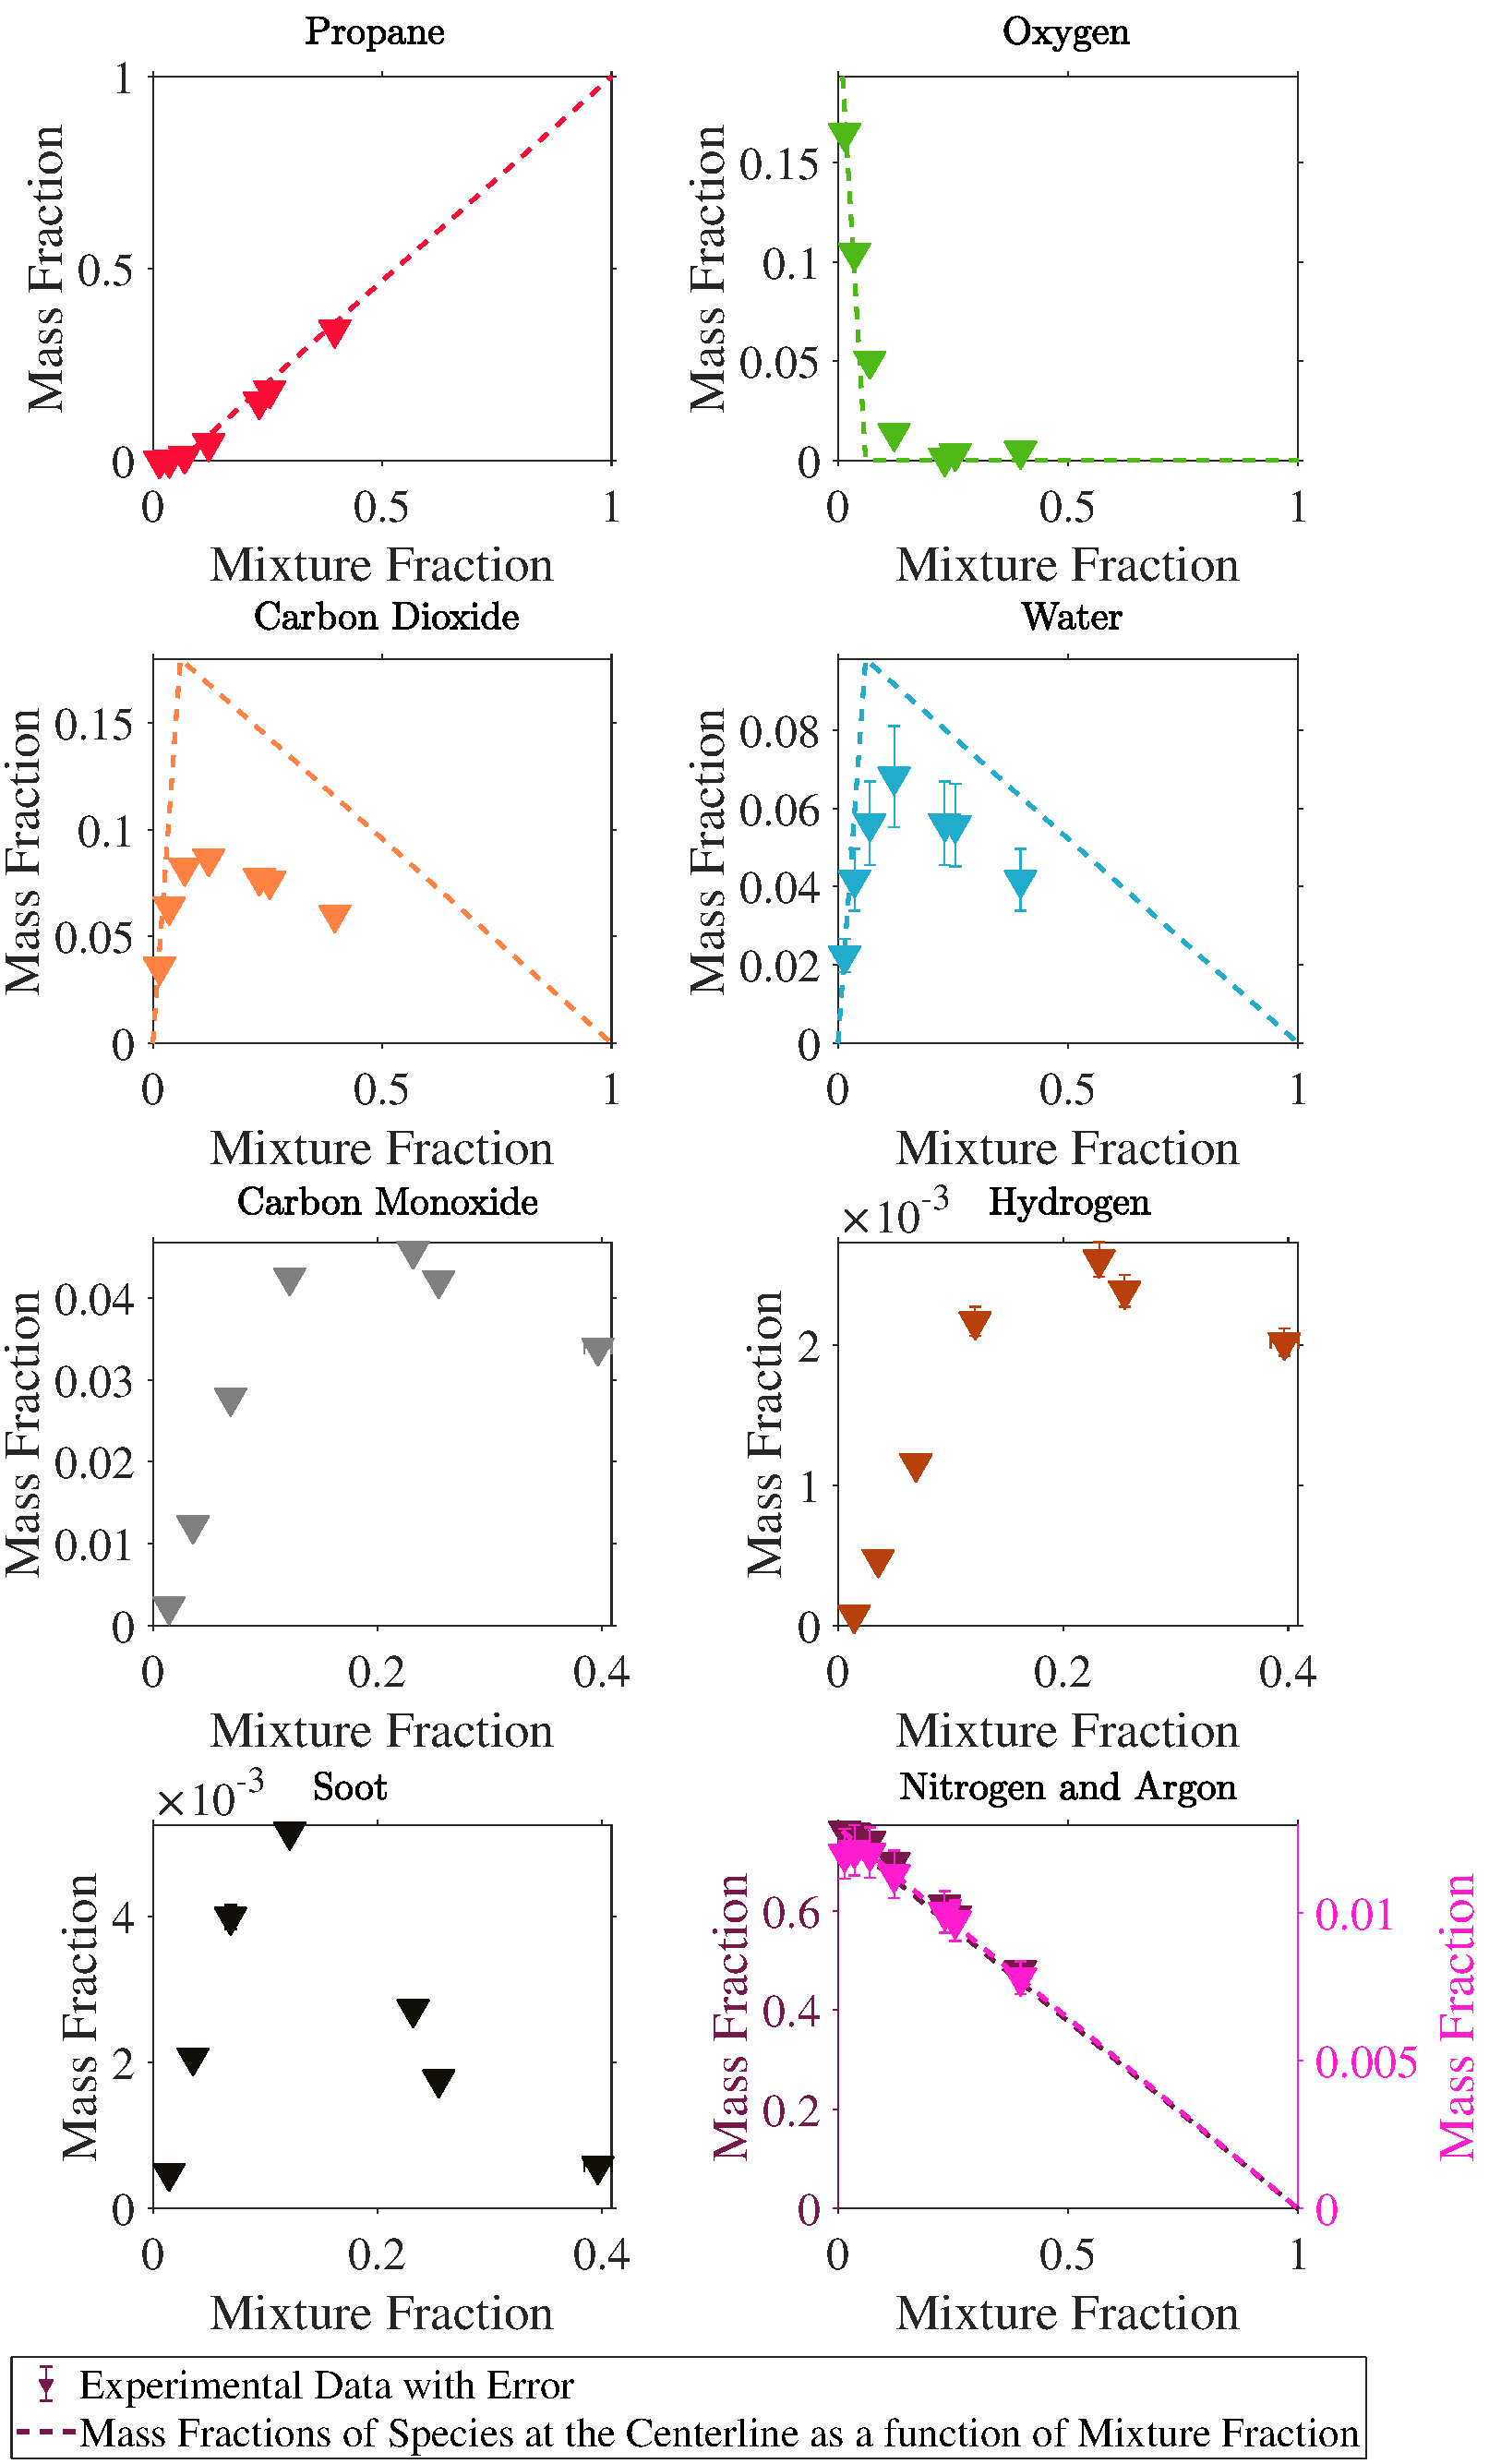
\includegraphics[width=10.5cm,keepaspectratio]{Propane 34KW_Mixture_Fraction_Major_Plot.pdf}
	\caption[Species mass fractions superimposed on propane (20 kW) state relations]{Plot of mass fractions, with uncertainty, of major species identified in the propane (34 kW) pool fire centerline as function of mixture fraction. The uncertainty is a combined uncertainty, discussed in further detail in Sections~\ref{sec:Uncertainty_Ver_Scheme} and \ref{sec:UncertaintyGasSpecies} for the mass fraction and mixture fractions, respectively.}
	\label{fig:Propane34KW_MIX_Frac_Major}
\end{figure}

\pagebreak

\section{Uncertainty Analysis of the Verification Scheme}\label{sec:Uncertainty_Ver_Scheme}

\subsection{Ratio of moles identified to moles injected }
\label{ssec:mole ratio}
The uncertainty of the ratio of the total number of moles identified by the TCD and MS, $n_{\rm tot}$, to the number of moles injected into the GC/MS, $n_{\rm inj}$, is calculated using the law of propagation of uncertainty and shown in the equation below:
\begin{equation}
\label{eq:mol_ratio_uncertainty}
u_{\scriptscriptstyle n_{\rm tot}/n_{\rm inj}} = \sqrt{\left(\frac{u_{\scriptscriptstyle n_{\rm tot}}}{n_{\rm inj}}\right)^2 + \left(\frac{-n_{\rm tot}~u_{\scriptscriptstyle n_{\rm inj}}}{{n_{\rm inj}^2}}\right)^2}
\end{equation}
The uncertainty of the total number of moles identified, $n_{\rm tot}$, is described in Section~\ref{ssec:Total Number of Moles Identified}. The uncertainty of the number of moles injected into the GC/MS, $n_{\rm inj}$, is described in Section~\ref{ssec:Total Moles Injected into the GC/MS for Calibation}.

\subsection{Carbon to Hydrogen Ratio}
\label{ssec:C2H_ratio}
The carbon to hydrogen ratio is calculated using Eq.~\ref{eq:c2h_ratio} using the mole fraction of any quantified gas species that contained either carbon or hydrogen.
\begin{equation}
\label{eq:c2h_uncertainty}
u_{\scriptscriptstyle {\rm C}/{\rm H}} =\frac{\textrm{W}_{\rm{C}}}{\textrm{W}_{\rm{H}}} \sqrt{{\sum\left(\frac{\partial ({\rm C}/{\rm H})}{\partial \bar{X}_{i}}\,u_{\scriptscriptstyle \bar{X}_{i}}~ \right)}^2+{\sum\left(\frac{\partial ({C}/{H})}{\partial X_{i}}\,u_{\scriptscriptstyle \bar{X}_{i}}\right)}^2}
\end{equation}
The uncertainty of the mass fractions of carbon and hydrogen containing species is described in Appendix~\ref{ssec:Uncertainty of Mass Fractions}.

\subsection{Inert Ratio}
\label{ssec:Inert_ratio}
%\begin{equation}
%\label{eq:inert_ratio}
%\rm{Inert~Ratio}=\frac{\bar{X}_{Ar}}{\bar{X}_{N_2}}
%\end{equation}
The inert ratio is calculated from the ratio the Nitrogen and Argon volume fractions, $\bar{X}_{N_2}$ and $\bar{X}_{Ar}$, identified by the TCD and TIC chromatograms. The uncertainty of inert ratio is determined from the law of propagation of uncertainty:
\begin{equation}
\label{eq:inert_ratio_uncertainty}
u_{\scriptscriptstyle \bar{X}_{Ar}/\bar{X}_{N_2}} = \sqrt{{\left(\frac{u_{\scriptscriptstyle \bar{X}_{Ar}}}{\bar{X}_{N_2}}\right)}^2+{\left(\frac{-\bar{X}_{Ar}u_{\scriptscriptstyle \bar{X}_{N_2}}}{\bar{X}_{N_2}}\right)}^2}
\end{equation}
The uncertainty of the volume fractions is described in Appendix~\ref{sec:UncertaintyMoleFrac}.

\subsection{Uncertainty Analysis of the Mixture Fraction}\label{sec:Uncertainty_Mix_Frac}

The mixture fraction, $Z$, is determined from Eq.~(\ref{eq:Mixture_Fraction}). The uncertainty of the mixture fraction is a function of the uncertainties in the carbon carrying species:
\begin{equation}
\label{eq:mixture_frac_uncertainty}
u_{\scriptscriptstyle Z}=\sqrt{{u_{\scriptscriptstyle \bar{Y}_{\rm F}}}^2+{\left(\frac{W_{\rm F}}{\rm x}\right)}^2{\sum_{i\ne {\rm F}}{\left(\frac{u_{\scriptscriptstyle \bar{Y}_{i}}}{\textrm{W}_{i}} \right)}^2}}
\end{equation}
The uncertainty of the mass fractions of carbon containing species is discussed in Appendix~\ref{ssec:Uncertainty of Mass Fractions}.

\pagebreak

\section{Previous Measurements in 30~cm Pool Fires}
Many experiments have been conducted on pool fires such as those considered in this report~\cite{Weckman1996,Kim2019,Hamins1994, Klassen1994,Hamins1991,Hamins2016,Wang2019,Buch1997,Hogben1998,Weckman1989,Corlett1966,Sung2019}.  Table~\ref{tab:pool_fire_prev_measurements} lists previously reported local and global measurements characterizing the structure of 30~cm diameter methanol, ethanol and acetone pool fires steadily burning under well-ventilated and quiescent conditions. These measurements complement each other and help build a more complete picture of the energetics, structure and dynamics of medium-scale pool fires burning oxygenated fuels. The accumulated information provides a basis for understanding details about these fires that makes them particularly suitable candidates for fire model evaluation. The three fires considered here are particularly useful as a testbed for radiation sub-models since blackbody radiation from soot is dependent on the fuel type. The time-averaged mean and RMS data from several of the studies is available through the Measurement and Computational Fire Phenomena (MaCFP) GitHub website~\cite{MaCFp}.

\begin{table}[!h]
    \centering
	\footnotesize
    \caption[List of previously measure pool fire parameters]{List of previously measured parameters obtained from a well-ventilated, round, steady, 30~cm diameter pool fires burning in a quiescent environment.}
    \label{tab:pool_fire_prev_measurements}
    \begin{tabular}{c|l|ccc}
    \hline
										& 								& \multicolumn{3}{c}{\textbf{References}} 	\\ \cline{3-5}
										&\raisebox{1.5ex}[0pt]{\textbf{Parameter}} 		& \textbf{Methanol}	& \textbf{Ethanol}	& \textbf{Acetone}		\\ \hline
\multirow{5}{*}{\rotatebox{90}{Global}} 				& Mass Loss Rate						&\cite{Hamins1991}	& 			&\cite{Hogben1998}		\\
										& Heat Release Rate					&\cite{Weckman1996}	& 			&\cite{Weckman1989}	\\
										& Mean Flame Height					&\cite{Kim2019,Klassen1994,Hamins1991,Buch1997}				&\cite{Kim2019,Hamins1991,Buch1997}					&	\cite{Kim2019,Buch1997,Hogben1998}		\\
										& Pulsation Frequency					&\cite{Weckman1996,Kim2019,Hamins1994,Klassen1994,Hamins1991,Hamins2016,Corlett1966}&	\cite{Kim2019,Buch1997,Corlett1966}			&	\cite{Kim2019,Buch1997,Weckman1989,Corlett1966}\\
										& Radiative Fraction					&\cite{Kim2019}	& \cite{Kim2019}	& \cite{Kim2019}		\\ \hline
\multirow{7}{*}{\rotatebox{90}{Local}}				& Radiative flux distribution on fuel surface 		&\cite{Hamins1994}	&			&		\\
										& Total Heat Flux Distributuion on Fuel Surface	&\cite{Kim2019}	& \cite{Kim2019}	& \cite{Kim2019}		\\
										& Radiative flux to surroundings 				&\cite{Kim2019,Klassen1994,Hamins1991}	&			&		\\
										& Transient fuel temperature 				&\cite{Hamins1994}	&			&		\\
										& Gas species volume fraction  				&\cite{Hamins2016}		&			&		\\
										& Local Gas Phase Temperature  				&\cite{Weckman1996,Hamins1991}				&			&		\\
										& Local Gas Phase Velocity  				&\cite{Weckman1996}				&			&		\\ \hline
    \end{tabular}
\end{table}

There are subtle differences in the experimental conditions as well as reporting assumptions and approximations that may account for some of the differences among the reported results. Some of the relevant issues are highlighted in Table~\ref{tab:Past_Pool_fire_parameters} below for the methanol, ethanol and acetone pool fires, respectively. The tables include information on the steady-state mass burning flux, $m''$, lip height, mean flame height. 

The radiative fraction to the surroundings including the fuel pool, $\chi_{\rm {rad}}$, and excluding the fuel pool, $\chi_{\rm{r}}$, during steady burning is reported for each study. $\chi_{\rm{rad}}$ is defined as the total radiative heat transfer to the surroundings and onto the fuel surface such that:
\begin{equation}
\label{eq:chi_rad}
\chi_{\rm{rad}}=\chi_{\rm{r}}+\chi_{\rm{sr}}
\end{equation}
where $\chi_{\rm{r}}$ is the integrated radiative flux emitted by the fire in all directions except to the fuel surface, normalized by the fire heat release rate. The term $\chi_{\rm{sr}}$ represents the integrated radiative flux emitted by the fire towards the fuel surface, normalized by the fire heat release rate. The values of the fractional enthalpy terms ($\chi_{\rm{r}}$, $\chi_{\rm{sr}}$) vary from fire to fire and are dependent on fuel type, burner diameter, and fire size. Ref.~\cite{Kim2019} describes the development of these terms in more detail.

There are several general considerations regarding the previous work:
\begin{itemize}
\item Ref.~\cite{Weckman1996} reports using a round, stainless-steel, 30.5~cm diameter burner, which differs from the 30.1~cm (inner) diameter burner used in Refs.~\cite{Kim2019,Hamins1994,Klassen1994,Hamins1991,Hamins2016,Wang2019,Buch1997}. Due to this disparity (3~\% in area), Table~\ref{tab:pool_fire_prev_measurements} refers to the mass burning flux (rather than the mass burning rate). The same circular, water-cooled, stainless-steel pan was used for experiments~\cite{Kim2019,Hamins1994,Klassen1994,Hamins1991,Hamins2016,Wang2019,Buch1997}. The burner had an inner diameter of 30.1~cm, a depth of 15~cm, and a wall thickness of 1.6~mm. The burner was fitted with legs such that the burner rim was positioned 30~c~m above the ground. The bottom of the burner was maintained at a constant temperature by flowing tap water (nominally 20~\si{\degree C}) through a 3~cm section on the bottom of the fuel pan. The exhaust flow in \cite{Kim2019} was 0.50~kg/s; this value can be assumed to be approximately the same for Refs.~\cite{Hamins1994,Klassen1994,Hamins2016,Wang2019,Buch1997}.
\item The lip height reported in Ref.~\cite{Weckman1996} and several of the other studies was 10~mm \cite{Hamins2016,Wang2019}, except Refs.~\cite{Hamins1994,Klassen1994,Hamins1991,Hamins2016,Buch1997} where it was reported as 4~mm or 5~mm (see Table~\ref{tab:pool_fire_prev_measurements}).
\item Weckman and Strong’s results \cite{Weckman1996} and Ref.~\cite{Hamins2016} are presented as a function of distance from the fuel surface, whereas all the other studies use the top of the burner rim as the point of reference.
\item A water-cooling section was not reported on the bottom of the burner used in Ref.~\cite{Weckman1996}; the burner in Refs.~\cite{Kim2019,Klassen1994,Hamins1991,Hamins1994,Hamins2016,Wang2019,Buch1997} had a water-cooling section on the bottom of the burner.
\item Refs.~\cite{Kim2019,Buch1997} reported radiative fraction emitted to the surroundings and did not include flux incident on the fuel surface; Ref.~\cite{Kim2019} reported radiative fraction to the surroundings plus flux incident on the fuel surface; Ref.~\cite{Klassen1994} assumed flux incident on the pool was uniform across the pool and equal to its value just outside the pool burner.
\item The amount of CO in the methanol, ethanol and acetone exhaust stream was below detection limits \cite{Kim2019}, so the combustion efficiency can be assumed to be about 1.
\item In Ref.~\cite{Klassen1994}, the average heat flux to the pool was assumed to be equal to the radiative flux measured just outside the burner, which is smaller than that expected \cite{Kim2019}. Here, $\chi_{\rm rad}$ is recalculated using $\chi_{\rm r}$= 0.065 from \cite{Kim2019}.
\item In Ref.~\cite{Klassen1994}, $\chi_{\rm rad}$ was based on a heat of combustion of 22.317~kJ/g. Here, $\chi_{\rm rad}$ is recalculated using the ``net'' heat of combustion (19.94 kJ/g) in which gaseous water is assumed to be the product of combustion \cite{Dippr}.
\item The heat of combustion values provided in Table~\ref{tab:Pool_Fire_Parameters_Table} were used to determine the heat release rates reported in Table~\ref{tab:Past_Pool_fire_parameters}.
\end{itemize}


\begin{table}[!h]
\begin{threeparttable}
    \centering
	\footnotesize
    \caption[Previously reported pool fire measurements]{Reported mass burning flux, $m''$, heat release rate, $\dot{Q}$, radiative fractions, excluding, $\chi_{\rm r}$, and including, $\chi_{\rm rad}$ the fuel pool, and the lip height of steady burning pool fires}
    \label{tab:Past_Pool_fire_parameters}
    \begin{tabular}{c|ccccp{0.3cm}cp{3cm}}
								&$\dot{m''}$~(\si{g/{m^2 s}})		& $\dot{Q}$~(\si{kW})	&  $\chi_{\rm r}$	& $\chi_{\rm rad}$	& Lip Height&\text{Ref.}				&\text{Comments}					\\ \hline
\multirow{11}{*}{\rotatebox{90}{Methanol}}	        	&	15.1				&	21.4				&			&			&	10		& \cite{Weckman1996}				&Volumetric Burning Rate of 1.35~\si{cm^3/s}	\\
		            					&	13.5~$\pm$~1.2		&	19.2				&	0.19		&0.24			&	10		&\cite{Kim2019}					&								\\
								&	12.9				&	18.3				&	0.22		&			&	5		&\cite{Hamins1994}				&Fuel Mass Burning Rate of 0.92~g/s			\\	
								&	12.6				&	18.0				&			&0.20			&	5		&\cite{Klassen1994}				&Fuel Mass Burning Rate of 0.9~g/s 			\\	           								
								&					&	20				&	0.18		&0.22			&	4		&\cite{Hamins1991}				&								\\
								&					&					&			&			&	5		&\cite{Hamins2016}				&								\\	
								&					&					&			&			&	10		&\cite{Wang2019}					&								\\
								&	12.8~$\pm$~1.3		&	18.2				&	0.22		&			&	5		&\cite{Buch1997}					&								\\
								&	12.4~$\pm$~0.5		&	17.6				&			&			&	10		&This study						&								\\
								&	12.4~$\pm$~0.5		&	17.6				&			&			&	10		&This study						&								\\
								&	13.2~$\pm$~0.4		&	18.7~$\pm$~0.6		&0.20~$\pm$~0.02&0.22~$\pm$0.2	&			& Average						&								\\ \hline
\multirow{4}{*}{\rotatebox{90}{Ethanol}}	        	&	16.2~$\pm$~1.8		&	31.0				&	0.21		&			&	10		&\cite{Kim2019}					&								\\
	        							&	14.4~$\pm$~1.4		&	27.3				&	0.16		&			&	5		&\cite{Buch1997}					&								\\
	        							&	13.9~$\pm$~2.1		&	26.3				&			&0.26			&	10		&This study						&								\\
								&	14.8~$\pm$~1.2		&	28.2~$\pm$~2.5		&0.19~$\pm$~0.3&0.26			&			& Average						&								\\ \hline
\multirow{5}{*}{\rotatebox{90}{Acetone}}	        	&	25.9				&	54.1				&	0.26		&			&	10		&\cite{Weckman1996}				&$\dot{Q''}$ of 740~\si{kW/m^2}			\\
	        							&	18.7~$\pm$~2.1		&	38.1				&	0.27		&0.31			&	10		&\cite{Kim2019}					&								\\
	        							&	18.7~$\pm$~1.9		&	37.7				&	0.28		&			&	5		&\cite{Buch1997}					&								\\
	        							&	17.6~$\pm$~2.6		&	35.5				&			&			&	10		&This Study						&								\\
								&	$18.3^{**}$~$\pm$~0.6	&	37.1~$\pm$~1.4		&0.27~$\pm$~0.1&0.31			&			& Average						&								\\ \hline
    \end{tabular}
    \begin{tablenotes}
      \footnotesize
	\item $^{**}$ The mass burning flux of acetone reported in \cite{Weckman1996} is an outlier and not included in the average.	
	\item Uncertainty of averages is defined as the standard deviation with a coverage factor of 2.
   	
    \end{tablenotes}
\end{threeparttable}
\end{table}
\end{document}
